\documentclass[a4paper, 10pt, twoside]{report}

%%%%%%%%%%%%%%%%%%%%%%%%%%%%%%%%%%%%%%%%%%%%%%%%%%%%%%%%%%%%%%%%%%%%%%%%%
\usepackage[babel, titelside, en]{ku-forside} % KU-forside
\usepackage[a4paper]{geometry}  % Geometri-pakke: Styrer bl.a. maginer    %
\usepackage[round]{natbib}
\usepackage{blindtext}
\usepackage{palatino}
\usepackage{mathpazo}
\usepackage[scaled]{helvet}
\usepackage{sectsty}
\usepackage{pgfplots}
\usepackage{amsmath}
\usepackage{amsthm}
\usepackage{gensymb}
\usepackage{tikz}
\usepackage{scrextend}
\usetikzlibrary{arrows,shapes,positioning}
\usepackage[format=plain, labelfont={small, sf, bf}, textfont={small, it}, singlelinecheck=off, margin={1cm, 0cm}, oneside, labelsep=newline]{caption}

% Change chapter headings to "Part"
\addto\captionsenglish{\renewcommand{\chaptername}{Part}}



% Change section headings
\sectionfont{\Large\sffamily}
\subsectionfont{\normalsize\sffamily}
\chapterfont{\sffamily}
\chapternumberfont{\huge\mdseries\sffamily}


% Put section numbers in margin
\makeatletter
\def\@seccntformat#1{\protect\makebox[0pt][r]{\csname
the#1\endcsname\quad}}
\makeatother

% allow text to not take up all space
\raggedbottom

% Enable definitions
\theoremstyle{definition}
\newtheorem{definition}{Definition}[section]
\newtheorem{theorem}{Theorem}[section]

% Math commands
\DeclareMathOperator*{\argmin}{arg\,min}
\DeclareMathOperator*{\expect}{\mathbb{E}}
\newcommand{\dtrain}{\mathcal{D}_{train}}
\newcommand{\dval}{\mathcal{D}_{val}}
\newcommand{\me}{\mathrm{e}}
\newcommand{\pderiv}[2]{\ensuremath\frac{\partial #1}{\partial #2}}
\newcommand{\emperror}[2]{\ensuremath\hat{E}(#1, #2)}
\newcommand{\trerror}[1]{\emperror{#1}{\dtrain}}
\newcommand{\valerror}[1]{\emperror{#1}{\dval}}
\renewcommand{\vector}[1]{\mathbf{#1}}
\renewcommand{\matrix}[1]{\vector{#1}}
\newcommand{\dotp}[2]{\ensuremath\vector{#1}^T\vector{#2}}
\newcommand{\augerror}{\ensuremath\bar{E}(\vector{w}, \dtrain)}
\newcommand{\hypspace}{\mathcal{H}}
\newcommand{\fspace}{\mathcal{X}}
\newcommand{\lspace}{\mathcal{Y}}
%
% Mini-manual til ku-forside pakken:
%
% Sprogmuligheder:     da, en
% babel loader babelpakken, med det valgte sprog
% Fakultetsmuligheder: farma, hum, jur, ku, life, nat, samf, sund, teo
% Farvemuligheder:     sh, farve
% Forsidemuligheder: lille, stor, titelside
%      titelside er identisk med designet p� ku.dk/designmanual
%      lille er giver et lille logo sammen med titlen p� den f�rste side
%      stor er giver et stort logo sammen med titlen p� den f�rste side
%
% Default er [da,nat,farve,titelside]
%
% Ex. \usepackage[babel, lille, jur, sh, en]{ku-forside} giver et lille logo i sorthvid for juridisk fakultet og loader babelpakken med engelsk som sprog.


\titel{Deep Multi-Task Learning} %
\undertitel{For Relation Extraction} %
\opgave{Master Thesis} % Findes kun under 'titelside'
\forfatter{Sune Andreas Dybro Debel}%
\dato{\today}%
\vejleder{Dirk Hovy} %  Findes kun under 'titelside'

\begin{document}
\maketitle
\thispagestyle{empty}
\newpage

\newgeometry{hmargin=4cm}
\begin{abstract}
\textit{In this thesis we investigate the usefulness of a multi-task, convolutional neural network architecture for relation classification. We review the relevant theoretical and practical research literature for relation classification, supervised machine learning, convolutional neural networks, and deep multi-task learning. We test a state-of-the-art multi-task convolutional neural network architecture designed for relation classification on the SemEval 2010 Task 8 dataset using several hard weight sharing strategies. We investigate the sample complexity dynamics of learning SemEval 2010 Task 8 simultaneously with other natural language processing tasks. We find that only one of the proposed weight sharing strategies lead to improvements in generalization performance of this target task. We identify potential causes for this difference in generalization performance across weight sharing strategies, and make recommendations for further experimentation in this direction.}
\end{abstract}

\pagebreak
\newgeometry{twoside, inner=4.8cm, outer=3.2cm, vmargin=3cm}

\addtocontents{toc}{\protect\thispagestyle{empty}}

\tableofcontents
\setcounter{page}{0}
\chapter{Introduction}

\section{Motivation}
The volume of digital text that exists in the world is rapidly increasing: The number of active science journals is growing with an annual rate of approximately 2.5\%. The total number of published articles in these journals grew from 1.8 in 2009 to 2.5 million in 2015 \citep{ware2009, ware2015}. Similar staggering growth rates can be cited for content produced by online newspapers, social media and digital documents generated by businesses \citep{perrin2015, mitchell2015}.
\\\\
Finding the right information at the right time in the face of this data volume is challenging. A significant reason is that information contained in digital text is in the form of natural language which is often cited as being \textbf{unstructured} (despite the fact that natural language is actually highly structured). Unstructured data can be understood as essentially the opposite of the kind of data we find in relational databases where every data item is associated with metadata such as column names and column types. This metadata makes the structured data easy to search and analyze with computers. In contrast, unstructured data such as text, images, sound and video is not.
\\\\
This problem has driven the development of so called \textbf{information extraction} techniques. The goal of these is to assign metadata to unstructured data, thereby giving some structure to it. This is an ambitious goal since in many cases it involves developing computer systems that perform tasks such as recognizing objects in images, converting speech to text or building data structures that capture the semantics of natural language, tasks we don't fully understand how humans are able to perform.
\\\\
\textbf{Relation extraction} is an information extraction task the goal of which is to automatically identify a fixed set of semantic relationships of interest such as \textit{Father-Son(Luke Skywalker, Darth Vader)} when they occur in natural language. Identifying these relations can significantly improve the quality of applications such as information retrieval or question answering systems \citep{jurafsky09}.

Like most other natural language processing problems, relation extraction is extremely challenging because of the high degree of variation and ambiguity of natural language. Relation extraction systems are therefore usually composed of composed of sub-systems that each solve a sub-problem of relation extraction. Specifically, most relation extraction systems proceed by first identifying the potential arguments such as \textit{Luke Skywalker} and \textit{Darth Vader} in our example for any relation of interest. The system then detects whether or not a relation does in fact exist between them, and finally classifies the relation if it exists.
\\\\
\textbf{Supervised machine learning} in general, and \textbf{deep learning} in particular, are very successful techniques for solving information extraction problems. These approaches are based on the idea of supplying examples of inputs such as text and corresponding correct outputs, so called labels, that we would like the system to reproduce given the input. The goal is to teach the system to give approximately correct output for new inputs that it hasn't seen before.
\\\\
The conditions under which supervised machine learning systems can be expected to give approximately correct answers are fairly well understood. Theoretical analysis shows that the number of training examples provided for the learning system is one of the main ingredients in this guarantee. Producing these examples can be costly however: It often requires a human annotator with specialized skills to provide the correct labels. This means there is significant motivation for reusing labeled training data to reduce the need to create large new collections of data for each new supervised machine learning problem.
\\\\
\textbf{Multi-task learning} is a technique for reusing labeled data \citep{caruana1997}. In essence, it relies on the idea that it may be easier to learn related tasks simultaneously than in isolation, or in other words, that a learning system that learns from previously annotated data may require fewer examples for learning a new task, thereby reducing the cost of data annotation.
\section{Problem Statement}
In this thesis we investigate multi-task learning for relation extraction. We focus on the relation classification step using deep learning techniques. Our goal is to investigate if and how learning an auxiliary task can benefit a target relation classification task that is learnt simultaneously, when the data available for the target task is limited. Specifically:
\begin{enumerate}
	\item We survey the relevant research literature in order to formally answer questions such as \textit{when is multi-task learning beneficial? How can we evaluate the usefulness of an auxiliary task?}
	\item We implement a deep multi-task learning relation classification system based on our research.
	\item We apply our theoretical understanding by analyzing our deep multi-task learning system for relation classification in order to make predictions about its performance.
	\item We empirically test our predictions about the system's performance using appropriate accuracy measures.
\end{enumerate}
In the following sections we detail the necessary background information necessary for understanding the relation extraction problem as well as our experiment with deep multi-task learning.
\chapter{Background}
\label{background}

In this part, we describe the information extraction problem and the challenges it poses. Moreover, we formally describe the supervised machine learning setting. Specifically, we discuss the challenges of noise and overfitting, and show the usefulness of Vapnik-Chervonenkis analysis. We also cover validation techniques for supervised machine learning systems and appropriate accuracy measures for evaluating information extraction systems.

\section{Information Extraction}
\label{information_extraction}
In natural language processing, information extraction is the problem of extracting structured information from unstructured text. Many practical information extraction problems fall in one of two categories: \textbf{named entity recognition} or \textbf{relation extraction} \citep{jurafsky09}. We introduce each of them in this section, and explain the challenges they pose.

\subsection{Named Entity Recognition}
\label{named_entity_recognition}
A named entity is roughly anything that has a proper name. The goal of named entity recognition is to label mentions of entities such as people, organizations or places occurring in natural language. The list of things these systems are tasked with recognizing is often extended to include things that aren't technically named entities such as amounts of money or calendar dates.

As an example, consider the sentence: 
$$
\text{Jim bought 300 shares of Acme Corp. in 2006.}
$$ 
A named entity recognition system designed to extract the entities \textit{person} and \textit{organization} should ideally assign the labels:
$$
	[\text{Jim}]_{person} \text{ bought 300 shares of } [\text{Acme Corp.}]_{organization} \text{ in 2006.}
$$
This is a difficult problem because of two types of ambiguity. Firstly, two distinct entities may share the same name and category, such as \textit{Francis Bacon} the painter and \textit{Francis Bacon} the philosopher. Secondly, two distinct entities can have the same name, but belong to different categories such as \textit{JFK} the former American president and \textit{JFK} the airport near New York. This means that named entity recognition systems need to have some model of the context in which these entities appear in order to produce correct output.
\\\\
Named entity recognition can be framed as a sequence labeling problem. A common approach is to apply so called tokenization to the text, i.e finding boundaries between words and punctuation, and associate each token with a label indicating which entity it belongs to. BIO-labeling (figure \ref{bio}) is a widely used labeling scheme in which token labels indicate whether the token is at the \textbf{B}eginning, \textbf{I}nside, or \textbf{O}utside an entity mention.
\begin{figure}
	\begin{center}
		\begin{tabular}{c c c c c c c c c c c}
	Jim & bought & 300 & shares & of & Acme & Corp & . & in & 2006 & . \\
	\texttt{B-PER} & \texttt{O} & \texttt{O} & \texttt{O} & \texttt{O} & \texttt{B-ORG} & \texttt{I-ORG} & \texttt{I-ORG} & \texttt{O} & \texttt{O} & \texttt{O}
	\end{tabular}
	\end{center}
	\caption{A sentence labeled with BIO labels for named entity recognition.}
	\label{bio}
\end{figure}

\subsection{Relation Extraction}
\label{relation_extract}
The goal of relation extraction is to identify relationships such as \textit{Family} or \textit{Employment} in natural language. The set of relations we would like a relation extraction system to recognize is commonly referred to as the \textbf{inventory}. Most often, the inventory is limited to relations between named entities. In some relation extraction tasks however, the goal is to more generally recognize relations between nouns \citep{hendrickx2009}. In both cases, the words between which a relation exists are referred to as the \textbf{arguments} of the relation.
\\\\
As an example, consider the sentence: 
$$
\text{Yesterday, New York based Foo Inc. announced their acquisition of Bar Corp.}
$$ 
Imagine we have designed a relation extraction system that recognizes the relation \textit{MergerBetween(organization, organization)} between two mentions of organizations. Ideally, we would like that system to extract the relation \textit{MergerBetween(Foo Inc., Bar Corp.)} from the above sentence.
\\\\
To simplify the relation extraction problem, it's often solved in three steps:
\begin{enumerate}
	\item \textbf{Named entity recognition} \enspace Identify the named entities in the input text.
	\item \textbf{Relation detection} \enspace For each pair of named entities in the input text, determine if a relation exists between them. This is a binary classification problem where the input is the text and the named entities detected in step 1, and the output is yes/no.
	\item \textbf{Relation classification} \enspace Classify each of the detected relations in the previous step. This a multi-label classification problem where the input is the input text and the named entities for which a relation was detected in step 2, and the output is a relation label.
\end{enumerate}
In this thesis we focus on step 3: assigning labels to detected relations. This is a difficult problem because of ambiguity. As an example, consider the sentence \textit{Susan left JFK}. Imagine that we want to design a relation extraction system that can detect the relations \textit{Physical(person, location): a person has a physical relation to a location} and \textit{Personal-Social(person, person): two persons have a social relation}. Both can reasonably be assigned the previous sentence, depending on whether \textit{JFK} refers to the airport near New York, or the former American president. Just as in named entity recognition, providing the correct label in this situation depends on context information.
\\\\
Early relation extraction systems relied on hand-crafted lexical and syntactic rules for detecting relations. \citet{hearst1992} is perhaps the earliest example of this approach. She considers the following sentence:
\begin{quote}
	\textit{Agar is a substance prepared from a mixture of red algae such as Gelidium for laboratory or industrial use.}
\end{quote}
Most people won't know what \textit{Gelidium} is. From the context we can infer that it's a type of algae however. She suggest that the following lexico-syntactic pattern between two noun phrases $NP_1$ and $NP_2$:
$$
NP_1\text{ such as }NP_2
$$
implies the relation $Hyponym(NP_1, NP_2)$. By performing a syntactic parse of the input sentence we can try to extract hyponym relations between noun phrases using such manually created rules. Because of the huge amount of variation found in natural languages, this is of course a cumbersome yet brittle approach.
\\\\
More recent solutions rely on supervised machine learning techniques to solve relation extraction problems. In this setting, a system learns to recognize relations in the inventory from annotated examples. The earliest examples of such systems relied on hand-crafted features of words in the neighborhood of the relation arguments, for example: \textit{the words between the arguments are "such as"} \citep{jurafsky09}. As we will see in part \ref{neural_networks}, the promise of avoiding complicated hand-crafted features of the sentence, but having the system learn useful lexico-syntactic features on its own is the major attraction of solutions based on neural networks.

\subsection{Accuracy Measures}
Information extraction systems are often evaluated empirically by applying them to collections of text, so called corpora, in which $N$ mentions of named entities or relations are known. In these tests, accuracy measures for each class $c$ of information we wish to extract are usually defined in terms of how many times the system correctly predicted class $c$. Most metrics use the following terminology:

\begin{center}
	\begin{tabular}{r | c c}
	 & \textbf{predicted as $c$} & \textbf{predicted as not $c$}  \\ \hline
	$c$ & True positives ($tp$) & False negatives ($fn$) \\
	\textbf{not} $c$ & False positives ($fp$) & True negatives ($tn$)
\end{tabular}
\end{center}
Where for example $tp$ is the number of true positives produced for class $c$.
\\\\
The distribution of labels used in both named entity recognition and relation extraction is often highly imbalanced. Consider for example the BIO labelling scheme for named entity recognition in figure \ref{bio}. Most words will be outside a mention of a named entity, and will have the label \texttt{O}. Using simple accuracy $\frac{tp + tn}{tp + tn + fn + fp}$ as a performance metric for a system that outputs bio labels for each token in the text is therefore not very informative, since a useless system which labels all tokens with \texttt{O} would achieve high performance.
\\\\
\textbf{Precision} and \textbf{recall} are more appropriate performance metrics for this reason. Precision $\frac{tp}{tp + fp}$ is the fraction of information items for which the system predicted class $c$ that actually belonged to class $c$.
Recall $\frac{tp}{tp + fn}$ on the other hand is the fraction of information items in the corpora of class $c$ that the system correctly extracted.
\\\\
In a multi-class classification problem we are forced to decide how to average these metrics across classes. Specifically, there are two ways of averaging an accuracy measure across $C$ different classes: micro and macro averaging \citep{sokolova2009}. In macro averaging, an accuracy measure is computed for each class $c$ separately, and then averaged across all $C$ classes. For example macro-precision $p_{M}$:
$$
p_{M} = \frac{1}{C}\sum_{c=1}^C p_c
$$
Where $p_c$ is the precision of the system for class $c$. Micro averaging on the other hand, averages an accuracy by accumulating $tp$, $tn$, $fp$ and $fn$ across all $C$ classes. For example micro-precision $p_{\mu}$:
$$
p_\mu = \frac{\sum\limits_{c=1}^C tp_c}{\sum\limits_{c=1}^C tp_c + fp_c}
$$
Where for example $tp_c$ is the true positives a system produces for class $c$.
\\\\
The main difference between macro and micro averages of accuracy measures is that micro averaging gives more weight to more frequent classes. In other words, micro averaging encodes the bias that infrequent classes are unimportant, and a misclassification of an example of such a class should not penalise the accuracy measure as much as a misclassification of a more frequent class. Whether on not this a reasonable bias depends on the problem. In order to be agnostic about the frequency of semantic relations we use macro averaging for all our reporting in this thesis.
\\\\
To get a single number that summarizes the performance, precision $p$ and recall $r$ are often combined into a single metric: the $F1$ measure. $F1$ is defined as the harmonic mean of precision and recall $\frac{2pr}{p + r}$. Variations that use the micro and macro versions of precision and recall can naturally be computed as the harmonic mean of the micro or macro precision and recall respectively.
\section{Supervised Machine Learning}
\label{supervised_machine_learning}

Most modern solutions to the information extraction problems in \ref{information_extraction} are based on supervised machine learning techniques. In this setting, a system learns to recognise the named entities or relations between them from examples provided by a human annotator. In this section we formally describe this approach and introduce important theoretical tools for understanding supervised machine learning.

\subsection{The Supervised Learning Problem}
\label{the_supervised_learning_problem}
A set $\mathcal{D}_{train}$ of $N$ training examples $(\mathbf{x}_i, \mathbf{y}_i)$ of inputs $\mathbf{x}_i$ and corresponding labels $\mathbf{y}_i$ is created by a human annotator. Each $\mathbf{x}_i$ belongs to an input space $\mathcal{X}$, for example the set of all english sentences. Each $\mathbf{y}_i$ belongs to a space $\mathcal{Y}$ of labels, for example the set of all sequences of BIO tags. As designers of the learning system, we specify the so called \textbf{hypothesis space} $\mathcal{H}$, a set of functions $h: \mathcal{X} \mapsto \mathcal{Y}$. We want to find a function $h \in \mathcal{H}$, sometimes called a \textbf{model} or \textbf{hypothesis}, that can automatically assign labels to a new set of un-labeled inputs $\mathcal{D}_{test} = \{ \mathbf{x}_i \mid \mathbf{x}_i \in \mathcal{X}\}$ at some point in the future. 

Supervised machine learning is the science of how to use an algorithm to find a function $h$ using $\mathcal{D}_{train}$ that performs well on $\mathcal{D}_{test}$, as measured by some performance measure $e$. In classification problems such as named entity recognition or relation extraction where $\mathcal{Y}$ is discrete, we typically use binary error $e(\mathbf{y}_1, \mathbf{y_2}) = \mathbb{I}[\mathbf{y}_1 \neq \mathbf{y}_2]$. Importantly, we are not explicitly interested in the performance of $h$ on $\mathcal{D}_{train}$ \citep{yaser12}.
\\\\
We can formalise the preference for functions $h$ that perform well on examples outside of the training set with a quantity known as \textbf{generalisation error}.

\begin{definition}[generalisation error] \label{generalisation_error}
	Let $P(\mathbf{x}, \mathbf{y})$ be a joint probability distribution over inputs $\mathbf{x} \in \mathcal{X}$ and labels $\mathbf{y} \in \mathcal{Y}$. Let $e(\mathbf{y}_1, \mathbf{y_2}) = \mathbb{I}[\mathbf{y}_1 \neq \mathbf{y}_2]$ be the binary error function that measures agreement between labels $\mathbf{y}_1$ and $\mathbf{y}_2$. Then the generalisation error $E$ of a function $h: \mathcal{X} \mapsto \mathcal{Y}$ is defined as:
	$$
		E(h) = \mathbb{E}_{\mathbf{x},\mathbf{y}\sim P(\mathbf{x}, \mathbf{y})}[e(h(\mathbf{x}), \mathbf{y})]
	$$
\end{definition}
Now, formally, the objective of supervised machine learning is to find a function $h^*$ in a space of functions $\mathcal{H}$ that minimises $E(h)$. We see the process generating the data as random, but with a behaviour describable by a distribution $P(\mathbf{x}, \mathbf{y})$. Unfortunately, this distribution is unknown, which makes $E$ unknown. However, we can use sampled data $\mathcal{D} = \{(\mathbf{x}, \mathbf{y}) \mid \mathbf{x}, \mathbf{y} \sim P(\mathbf{x}, \mathbf{y})\}$ to estimate $E(h)$ with a quantity known as \textbf{empirical error}:

\begin{definition}[empirical error] \label{empirical_error}
	Let $\mathcal{D}$ be a set of $N$ examples $\{(\mathbf{x}_i, \mathbf{y}_i) \mid \mathbf{x}_i, \mathbf{y}_i \sim P(\mathbf{x}, \mathbf{y})\}$. Then the empirical error $\hat{E}$ is defined as:
	$$
		\hat{E}(h, \mathcal{D}) = \frac{1}{N}\sum\limits_{i=1}^N e(h(\mathbf{x}_i), \mathbf{y}_i)
	$$
\end{definition}

Because $\mathcal{D}$ is a random quantity, it's dangerous to use $\hat{E}$ to estimate $E$. We risk that the samples are not representative of $P(\mathbf{x}, \mathbf{y})$, leading us to believe that $h$ is great, when in fact it's terrible. We can bound the probability that $\hat{E}$ is a bad estimate of $E$ if we make two assumptions:

Firstly, we assume that the samples in $\mathcal{D}$ are drawn independently from $P(\mathbf{x}, \mathbf{y})$, that is observing any one sample did not change the probability of observing any other sample.

Secondly, we assume that $h$ is independent of $\mathcal{D}$, in other words, that $h$ was not specifically chosen based on the sample. These assumptions enable us to apply \textbf{Hoeffding's inequality} to bound the probability that $\hat{E}$ is far away from $E$:

\begin{theorem}[Hoeffding's inequality]
	let $E(h)$ be defined as in definition \ref{generalisation_error}, and let $E(h, \mathcal{D})$ be defined as in definition \ref{empirical_error}. Then:
	$$
	\mathbb{P}\left( |E(h) - \hat{E}(h, \mathcal{D})| \geq \epsilon \right) \leq 2e^{-2N\epsilon^2}
	$$
\end{theorem}

The inequality tells us that the probability that $E$ is more than $\epsilon$ away from $\hat{E}$ decreases exponentially in $\epsilon$ and $N$. In other words, the more samples in $D$, the less likely it is that $E$ will be misleading.
\\\\
Estimating $E$ with a sample that is independent of $h$ is a technique called \textbf{validation}. In validation, the sample provided by a human annotator is split into two datasets, $\mathcal{D}_{train}$, which we intend to use to search for $h^*$, and $\mathcal{D}_{validate}$, which saved until we are done searching. Since $\mathcal{D}_{validate}$ is independent of whichever $h$ we selected, Hoeffding's inequality applies and $\mathcal{D}_{validate}$ can be used to estimate $E$.
\\\\
Because $\mathcal{D}_{train}$ is used to select $h$, it cannot be used to estimate $E$ by Hoeffding's inequality, and we need more sophisticated techniques to understand the relationship between $\mathcal{D}_{train}$ and $E$. The central question in supervised machine learning is \textit{how can we best define $\mathcal{H}$ and use $\mathcal{D}_{train}$ to make $E$ small?} Answering this question is the objective of a field of research known as \textbf{statistical learning theory}.

\subsection{Validation}

\subsection{Statistical Learning Theory}
\label{statistical_learning_theory}
We would like to know how best to define $\mathcal{H}$ and use $\mathcal{D}_{train}$ in order to make $E$ small. $\mathcal{D}_{train}$ is the only information we have about $P(\mathbf{x}, \mathbf{y})$, and therefore also the only information we have about $E$. A straight-forward idea would be to find a function $g \in \mathcal{H}$ that minimises the \textbf{training error} $\hat{E}(g, \mathcal{D}_{train})$ in the hope that $g$ will also minimise $E$. 

As we argued in section \ref{supervised_machine_learning}, using $\hat{E}$ to estimate $E$ can be misleading. Moreover, because $D_{train}$ is used to specifically choose $g$ that makes $\hat{E}$ small, the guarantees provided by Hoeffding's inequality no longer holds, and therefore it may be possible to select $g$ such that $\hat{E}(g, \mathcal{D}_{train})$ is small and $E(g)$ is large, even when we have a large number of training examples.

The phenomena where training error is small but generalisation error is large is known as \textbf{overfitting}. As the name implies, it's caused by harmful idiosyncrasies of $\mathcal{D}_{train}$ that, when used to minimise $\hat{E}(h, \mathcal{D}_{train})$, leads us to a $g$ with a larger $E$ than other functions in $\mathcal{H}$. These idiosyncrasies of $\mathcal{D}_{train}$ are ultimately the product of \textbf{noise}.
\\\\
In general, noise comes in two forms. The first form is known as \textbf{stochastic noise}. This type of noise is introduced by variation in the relationship between $\mathbf{x}$ and $\mathbf{y}$ that is inherently unpredictable. For example, human error is a common source of stochastic noise in information extraction, where an annotator incorrectly labels a piece of text. Selecting a $g$ that repeats this error is a case of overfitting, because $g$ will have lower training error but larger generalisation error than another $h$ that doesn't predict the incorrect annotation, since presumably the error is the exception to the rule.
\\\\
The second type of noise is called \textbf{deterministic noise}. This type of noise may be introduced when the relationship between $\mathbf{x}$ and $\mathbf{y}$ is deterministic, but $\mathcal{H}$ doesn't have the capacity to represent this relationship exactly.

To understand deterministic noise, imagine that even $h^*$ can't represent the deterministic relationship $\mathbf{y} = f(\mathbf{x})$ exactly. Suppose that we get a $\mathcal{D}_{train}$ that contains a sample $(\mathbf{x}_i, \mathbf{y}_i)$ that falls outside the capacity of $h^*$, that is, $h^*(\mathbf{x}_i) \neq \mathbf{y}_i$. Now further imagine that in order to minimise $\hat{E}$, we select a $g$ that predicts this sample, such that $h(\mathbf{x}_i) = \mathbf{y}_i$. This is a case of overfitting since we know that there is at least one function in $\mathcal{H}$ with lower generalisation error than $g$, namely $h^*$.
\\\\
The risk of overfitting is linked to the diversity of $\mathcal{H}$. By diversity of $\mathcal{H}$, we roughly mean how different any function in $\mathcal{H}$ is from any other function in $\mathcal{H}$. The more diverse $\mathcal{H}$ is, the greater the risk that there exists a $h \in \mathcal{H}$ that will overfit $\mathcal{D}_{train}$.

A \textbf{dichotomy} is a central concept in measuring the diversity of $\mathcal{H}$. A dichotomy is a specific sequence of $N$ labels. For example, if $\mathcal{Y} = \{0, 1\}$, and $N = 3$, then (0 1 0) is a dichotomy, and so is (1 0 0). We have listed all dichotomies for $N = 3$ in figure \ref{dichotomies}.

\begin{figure}[h]
	\begin{center}
			\begin{tabular}{c}
		(0 0 0) \\
		(1 0 0) \\
		(0 1 0) \\
		(0 0 1) \\
		(1 1 0) \\
		(0 1 1) \\
		(1 0 1) \\
		(1 1 1) \\
	\end{tabular}
	\end{center}
	\caption{All dichotomies for $\mathcal{Y} = \{0, 1\}$ and $N = 3$. There are $2^3 = 8$ ways to choose a sequence of 3 labels from 2 possibilities.}
	\label{dichotomies}
\end{figure}

Dichotomies allow us to group similar functions. In the rest of this section, let's assume that $\mathcal{Y} = \{0, 1\}$. By simple combinatorics the number of dichotomies for $N$ must be smaller than or equal to $2^N$. There may be infinitely many functions in $\mathcal{H}$, but on a specific $\mathcal{D}_{train}$, many of them will produce the same dichotomy since the number of training examples in $\mathcal{D}_{train}$ is finite.
This allows us to quantify the diversity of $\mathcal{H}$ in terms of the number of dichotomies it's able to realise on a set of $N$ points. This is achieved by a measure known as the \textbf{growth function}.
\begin{definition}[growth function]
	\label{growth_function}
	Let $\mathcal{H}(N) = \{(h(\mathbf{x}_1), \dots, h(\mathbf{x}_N))\ \mid h \in \mathcal{H}, \mathbf{x}_i \in \mathcal{X}\}$ be the set of all dichotomies generated by $\mathcal{H}$ on $N$ points, and let $|\cdot|$ be the set cardinality function. Then the growth function $m$ is:
	$$
		m(N, \mathcal{H}) = \max |\mathcal{H}(N)|
	$$
\end{definition}
In words, the growth function measures the maximum number of dichotomies that are realisable by $\mathcal{H}$ on $N$ points. To compute $m(N, \mathcal{H})$, we consider any choice of $N$ points from the whole input space $\mathcal{X}$, select the set that realises the most dichotomies and count them.
\\\\
The growth function allows us to account for redundancy in $\mathcal{H}$. If two functions $h_i \in \mathcal{H}$ and $h_j \in \mathcal{H}$ realise the same dichotomy on $\mathcal{D}$, then any statement based only on $\mathcal{D}$ will be either true or false for for both $h_i$ and $h_j$. This makes it possible to group the events \textit{$\hat{E}(h_i, \mathcal{D})$ is far away from $E(h_i)$} and \textit{$\hat{E}(h_j, \mathcal{D})$ is far away from $E(h_j)$}, and thereby avoiding to overestimate the probability of the union of both events occurring.

If $\mathcal{H}$ is infinite, the number of redundant functions in $\mathcal{H}$ will also be infinite, since the number of dichotomies on $N$ points is finite. If $m(N, \mathcal{H})$ is much smaller than $2^N$, the number of redundant functions in $\mathcal{H}$ will be so large as to make the probability that $\hat{E}$ is far away from $E$ very small.
\\\\
 This line of reasoning is the basis of the Vapnik-Chervonenkis bound, which bounds $E(h)$ in terms of $\hat{E}(h, \mathcal{D}_{train})$:

\begin{theorem}[Vapnik-Chervonenkis bound]
	\label{vc_bound}
	Let $m(N, \mathcal{H})$ be defined as in definition \ref{growth_function}, $E(h)$ as \ref{generalisation_error}, and $\hat{E}(h, \mathcal{D})$ as in \ref{empirical_error}. Then, with probability $1 - \delta$:
	$$
	E(h) \leq \hat{E}(h, \mathcal{D}_{train}) + \sqrt{\frac{8}{N}\ln \frac{4m(2N, \mathcal{H})}{\delta}}
	$$
\end{theorem}
The bound tells us that $E(h)$ will be close to $\hat{E}(h, \mathcal{D}_{train})$ if $m(N, \mathcal{H})$ is small and $N$ is large. Intuitively, this tells us that a set $\mathcal{H}$ that contains "simple" functions will make it easier to choose $g$ such that generalisation error will be close to training error, where simple means: functions that realise a small number of dichotomies.

On the other hand, having a set $\mathcal{H}$ that can realise a large number of dichotomies on $N$ points, will make it easier to find a function that will make $\hat{E}(h, \mathcal{D}_{train})$ small. Using a $\mathcal{H}$ with functions that are too simple is called \textbf{underfitting}. It occurs when we search for a function in the set of functions $\mathcal{H}$, when there is another, more diverse set of functions $\mathcal{G}$ which contain a function with lower generalisation error.
\\\\
This analysis tells us that an optimally diverse $\mathcal{H}$ balances the tradeoff between the risk of overfitting, represented in the bound by $m$, and the risk of underfitting, represented by $\hat{E}$. In practice, underfitting is less of a problem than overfitting, since modern supervised machine learning algorithms search in extremely diverse spaces of functions $\mathcal{H}$. In fact, most $\mathcal{H}$ are so diverse that steps must be taken to avoid minimising $\hat{E}$ as much as is actually possible. These techniques are known as \textbf{regularisation}, which we will see an instance of in section \ref{early_stopping}.

\section{Summary}
In this section we have seen that the purpose of named entity recognition is to identify mentions of entities such as people, organizations and places in natural language. The purpose of relation extraction systems is to identify relationships between them. 

We have seen that simple accuracy is uninformative as an evaluation measure in information extraction, and described precision and recall as alternative metrics.

We have described the formal setting of supervised machine learning. We have discussed concepts such as overfitting and noise, diversity of the set of functions $\mathcal{H}$ from which to choose $h$, and its impact on training and generalization error. Finally we have discussed validation as a technique for estimating $E$ empirically.

\chapter{Neural Networks}
\label{neural_networks}

\section{Feed-Forward Neural Networks}
A feed-forward neural network is a function $h: \mathcal{X} \mapsto \mathcal{Y}$. To understand how it works, it's instructive to look at each part of its name in isolation.
\\\\
$h$ is called a \textbf{network} because it's a composition of $L$ \textbf{layers} of other functions $f^{(l)}$. Each $f^{(l)}$ receives input from $f^{(l-1)}$. For example if $L = 2$, then $h(\mathbf{x}) = f^{(2)}(f^{(1)}(\mathbf{x}))$. We denote the input to $f^{(1)}$ as $\mathbf{x}^{(0)}$, which is identical to the input vector $\mathbf{x}$, except for an added \textbf{bias} component of 1, as described later in this section. each $f^{(l)}$ outputs a vector $\mathbf{x}^{(l)}$ of dimension $d^{(l)}$ which is the input of $f^{(l+1)}$. The dimensionality of these vectors determine the \textbf{width} of the network. The number of layers $L$ is called the \textbf{depth} of the network. $f^{(L)}$ is called the \textbf{output layer}. The remaining functions $f^{(1)}$ to $f^{(L-1)}$ are called \textbf{hidden layers}. 
\\\\
The functions $f^{(1)}$ to $f^{(L)}$ are ordered by their index $l$. By ordered, we mean that the index of the innermost functions are smaller than the index of the outermost. $h$ is called a \textbf{feed-forward} network because each $f^{(l)}$ can receive input only from functions $f^{(i)}$ if $l > i$. In other words, it's not possible for a function $f^{(l)}$ to feed its own output into itself, or any other function that it receives input from.
\\\\
Finally $h$ is called a \textbf{neural} network since its design is loosely based on neurons in the brain \citep{goodfellow16}. Each component $x_i$ of the vector $\mathbf{x}^{(l)}$ can be seen as the output of a unit similar to a neuron. Each unit in layer $l$ receives input from units in layer $l-1$. The output $x^{(l-1)}_i$ of unit $i$ in layer $l-1$ is multiplied by a weight $w^{(l)}_{ij}$ that gives the strength of the connection between unit $i$ in $l-1$ and unit $j$ in $l$. Unit $j$ sums all of the input it receives from units in layer $l-1$ to obtain its \textbf{activation} $a^{(l)}_j = \sum_{i=0}^{d^{(l-1)}} w^{(l)}_{ij}x^{(l-1)}_{i}$. To compute its output $x^{(l)}_j$, it applies an \textbf{activation function} $\sigma(a^{(l)}_j)$ to its activation.

Activation functions model the behaviour of biological neurons by outputting a signal only when the activation is above a certain threshold. To make it possible to learn this threshold for each unit using the same activation function, we introduce a special \textbf{bias} unit that always outputs 1. The index of the bias unit in layer $l$ is 0 by convention. Figure \ref{connection}. shows how a unit $j$ computes its output $x^{(l)}_j$ by combining the outputs of units in layer $l-1$.

\tikzstyle{neuron}=[circle,draw,minimum size=20pt,inner sep=0pt]
\tikzstyle{summation} = [square, minimum size=20pt,inner sep=0pt]
\tikzstyle{edge} = [draw,thick,-]
\tikzstyle{weight} = [font=\small]

\begin{figure}[h]
	\centering
	\begin{tikzpicture}[->, >=stealth, swap]
			\node [neuron] (sigma1) at (0,0) {$i$};
			\node [neuron] (sigma2) at (6,0) {$j$};
			\node [neuron] (bias1) at (0,1) {$1$};
			\node []       (z1)      at (1,-.4) {$x^{(l-1)}_i$};
			\node []       (w)     at (3,-.4) {$w^{(l)}_{ij}$};
			\node []       (w)     at (3,.9) {$w^{(l)}_{0j}$};
			\node []       (aw)   at (5,-.4) {$a^{(l)}_j$};
			\node []	   (empty) at (8,0) {};
			\node []       (z2)    at (7,-.4) {$x^{(l)}_j$};
		
			\draw (sigma1) edge (sigma2);
			\draw (sigma2) edge (empty);
			\draw (bias1) edge (sigma2);
	\end{tikzpicture}
	\caption{A visual representation of the connections between unit $i$ in layer $l-1$, the bias unit in $l-1$, and unit $j$ in layer $l$. The connection strength between these units is given by the weight $w^{(l)}_{ij}$ between $i$ and $j$, and $w^{(l)}_{0j}$ between the bias unit and $j$. The activation $a^{(l)}_j$ at unit $j$ is computed by $a^{(l)}_j = w^{(l)}_{ij}x^{(l)}_i + w^{(l)}_0$. The output $x^{(l)}_j$ of unit $j$ is given by $x^{(l)}_j = \sigma(a^{(l)}_j)$}
	\label{connection}
\end{figure}
\noindent
Keeping track of the indices $l$, $i$ and $j$ quickly becomes confusing. By collecting all of the weights of connections going into unit $j$ in layer $l$ in a vector $\mathbf{w}^{(l)}_j$, the activation at unit $j$ can be computed as a dot product $a^{(l)}_j = {\mathbf{w}^{(l)}_j} \cdot \mathbf{x}^{(l-1)}$. Moreover, we can compute the entire vector $\mathbf{a}^{(l)}$ of activations at layer $l$, by organising the weight vectors $\mathbf{w}^{(l)}_j$ in a matrix $\mathbf{W}^{(l)} = \begin{bmatrix} \mathbf{w}^{(l)}_1 & \dots & \mathbf{w}^{(l)}_{d^{(l)}} \end{bmatrix}^T$, which leads to $\mathbf{a}^{(l)} = \mathbf{W}^{(l)}\mathbf{x}^{(l-1)}$.
\\\\
By gathering the weights in matrices $\mathbf{W}^{(l)}$, we have simplified our view of $h$ into a composition of matrix-vector products and element-wise application of activation functions. Figure \ref{neural_network} shows the parallel views of neural networks as networks of units and matrix-vector operations.

\begin{figure}[h]
	\centering
	\begin{tikzpicture}[->, >=stealth, swap]
		\node [neuron] (bias0)   at (0, 2)  {1};
		\node [neuron] (x1)      at (0, 1)  {$x_1$};
		\node [neuron] (x2)      at (0, 0)  {$x_2$};
		\node []       (x)       at (0,-1)  {$\mathbf{x}^{(0)}$};
		\node [neuron] (bias1)   at (4, 2)  {1}; 
		\node [neuron] (sigma11) at (4, 1)  {$\sigma$};
		\node [neuron] (sigma12) at (4, 0)  {$\sigma$};
		\node []       (layer1)  at (4,-1)  {$\sigma(\mathbf{W}^{(1)} \mathbf{x}^{(0)}) = \mathbf{x}^{(1)}$};
		\node [neuron] (sigma21) at (8, 1)  {$\sigma$};
		\node [neuron] (sigma22) at (8, 0)  {$\sigma$};
		\node []       (layer2)  at (8,-1)  {$\sigma(\mathbf{W}^{(2)} \mathbf{x}^{(1)}) = h(\mathbf{x})$};
		\node []	   (empty1)  at (9, 1) {};
		\node []       (empty2)  at (9, 0) {};   
		
		
		\draw (bias0)   edge (sigma11);
		\draw (x1)      edge (sigma11);
		\draw (x2)      edge (sigma11);
		\draw (bias0)   edge (sigma12);
		\draw (x1)      edge (sigma12);
		\draw (x2)      edge (sigma12);
		\draw (bias1)   edge (sigma21);
		\draw (sigma11) edge (sigma21);
		\draw (sigma12) edge (sigma21);
		\draw (bias1)   edge (sigma22);
		\draw (sigma11) edge (sigma22);
		\draw (sigma12) edge (sigma22);
		\draw (sigma21) edge (empty1);
		\draw (sigma22) edge (empty2);
	\end{tikzpicture}
	\caption{A visual representation of $h(\mathbf{x}) = f_2(f_1(\mathbf{x}^{(0)}))$. The activation at each layer $\mathbf{a}^{(l)}$ is computed by $\mathbf{W}^{(l)}\mathbf{x}^{(l-1)}$. The output at each layer is computed by element-wise application of the activation function of $\sigma(\mathbf{a}^{(l)})$.}
	\label{neural_network}
\end{figure}
\noindent
We now have all the components we need to specify $\mathcal{H}$ as a set of neural networks. The set is defined by the depth of the networks $L$, the number of units in each layer $d_l$ , and the activation function $\sigma$.
For a particular $L$, $d_l$, and $\sigma$, each $h \in \mathcal{H}$ corresponds exactly to a unique assignment of real numbers to all of its weights. We can make the dependence of $h$ on its weights explicit by defining a vector $\mathbf{w} = \begin{bmatrix} w^{(1)}_{ij} & \dots & w^{(L)}_{ij}\end{bmatrix}$ and writing $h(\mathbf{x}, \mathbf{w})$ which means \textit{the function $h$ parameterised by the weight vector $\mathbf{w}$}. In the next section we discuss how to choose the activation functions at the layers of the network.

\subsection{Activation Functions}
\label{activation_functions}
Activation functions mimic the behaviour of neurons in the brain. A neuron emits a signal when the combined input it receives from other neurons exceeds a certain threshold. Activation functions achieve this by a variation of the step function, where an activation signal $a^{(l)}_j$ below the threshold is mapped to a value near zero, and an activation signal above the threshold is mapped to a value greater than zero. From a mathematical perspective, the role of activation functions is to introduce non-linearity in $h$, which allows it to approximate a much larger class of functions.
\\\\
Many networks use \textbf{sigmoid} activation functions such as the classical sigmoid function $\sigma(a) = \frac{1}{1 + \me^-a}$. These functions have the advantage of being differentiable everywhere. As we will see in section \ref{learning_algorithm}, differential calculus is the fundamental tool for finding a good $h \in \mathcal{H}$, which makes differentiability a desirable quality. One drawback of sigmoid activation functions is that their derivates are small, as seen in figure \ref{sigmoid}. For example, we can show that $\max \frac{d\sigma}{da} = \frac{1}{4}$. As we will see in section \ref{learning_algorithm}, neural networks are trained by multiplying chains of derivatives. When these derivatives are smaller than 1, the magnitude of the derivative shrinks in the length of the chain of terms which can make learning from $\mathcal{D}_{train}$ extremely slow.
\begin{figure}
	\centering
	%% Creator: Matplotlib, PGF backend
%%
%% To include the figure in your LaTeX document, write
%%   \input{<filename>.pgf}
%%
%% Make sure the required packages are loaded in your preamble
%%   \usepackage{pgf}
%%
%% Figures using additional raster images can only be included by \input if
%% they are in the same directory as the main LaTeX file. For loading figures
%% from other directories you can use the `import` package
%%   \usepackage{import}
%% and then include the figures with
%%   \import{<path to file>}{<filename>.pgf}
%%
%% Matplotlib used the following preamble
%%   \usepackage{fontspec}
%%   \setmainfont{Palatino}
%%   \setsansfont{Lucida Grande}
%%   \setmonofont{Andale Mono}
%%
\begingroup%
\makeatletter%
\begin{pgfpicture}%
\pgfpathrectangle{\pgfpointorigin}{\pgfqpoint{4.614828in}{3.237168in}}%
\pgfusepath{use as bounding box, clip}%
\begin{pgfscope}%
\pgfsetbuttcap%
\pgfsetmiterjoin%
\definecolor{currentfill}{rgb}{1.000000,1.000000,1.000000}%
\pgfsetfillcolor{currentfill}%
\pgfsetlinewidth{0.000000pt}%
\definecolor{currentstroke}{rgb}{1.000000,1.000000,1.000000}%
\pgfsetstrokecolor{currentstroke}%
\pgfsetdash{}{0pt}%
\pgfpathmoveto{\pgfqpoint{0.000000in}{-0.000000in}}%
\pgfpathlineto{\pgfqpoint{4.614828in}{-0.000000in}}%
\pgfpathlineto{\pgfqpoint{4.614828in}{3.237168in}}%
\pgfpathlineto{\pgfqpoint{0.000000in}{3.237168in}}%
\pgfpathclose%
\pgfusepath{fill}%
\end{pgfscope}%
\begin{pgfscope}%
\pgfsetbuttcap%
\pgfsetmiterjoin%
\definecolor{currentfill}{rgb}{1.000000,1.000000,1.000000}%
\pgfsetfillcolor{currentfill}%
\pgfsetlinewidth{0.000000pt}%
\definecolor{currentstroke}{rgb}{0.000000,0.000000,0.000000}%
\pgfsetstrokecolor{currentstroke}%
\pgfsetstrokeopacity{0.000000}%
\pgfsetdash{}{0pt}%
\pgfpathmoveto{\pgfqpoint{0.074056in}{0.375732in}}%
\pgfpathlineto{\pgfqpoint{4.559273in}{0.375732in}}%
\pgfpathlineto{\pgfqpoint{4.559273in}{3.237168in}}%
\pgfpathlineto{\pgfqpoint{0.074056in}{3.237168in}}%
\pgfpathclose%
\pgfusepath{fill}%
\end{pgfscope}%
\begin{pgfscope}%
\pgfpathrectangle{\pgfqpoint{0.074056in}{0.375732in}}{\pgfqpoint{4.485217in}{2.861436in}} %
\pgfusepath{clip}%
\pgfsetrectcap%
\pgfsetroundjoin%
\pgfsetlinewidth{1.003750pt}%
\definecolor{currentstroke}{rgb}{0.000000,0.000000,1.000000}%
\pgfsetstrokecolor{currentstroke}%
\pgfsetdash{}{0pt}%
\pgfpathmoveto{\pgfqpoint{0.074056in}{0.375850in}}%
\pgfpathlineto{\pgfqpoint{0.522578in}{0.376604in}}%
\pgfpathlineto{\pgfqpoint{0.724412in}{0.377877in}}%
\pgfpathlineto{\pgfqpoint{0.858969in}{0.379637in}}%
\pgfpathlineto{\pgfqpoint{0.971099in}{0.382164in}}%
\pgfpathlineto{\pgfqpoint{1.060804in}{0.385316in}}%
\pgfpathlineto{\pgfqpoint{1.128082in}{0.388652in}}%
\pgfpathlineto{\pgfqpoint{1.195360in}{0.393142in}}%
\pgfpathlineto{\pgfqpoint{1.240212in}{0.396965in}}%
\pgfpathlineto{\pgfqpoint{1.285064in}{0.401620in}}%
\pgfpathlineto{\pgfqpoint{1.329917in}{0.407282in}}%
\pgfpathlineto{\pgfqpoint{1.374769in}{0.414164in}}%
\pgfpathlineto{\pgfqpoint{1.419621in}{0.422520in}}%
\pgfpathlineto{\pgfqpoint{1.464473in}{0.432652in}}%
\pgfpathlineto{\pgfqpoint{1.486899in}{0.438494in}}%
\pgfpathlineto{\pgfqpoint{1.509325in}{0.444919in}}%
\pgfpathlineto{\pgfqpoint{1.531751in}{0.451982in}}%
\pgfpathlineto{\pgfqpoint{1.554177in}{0.459742in}}%
\pgfpathlineto{\pgfqpoint{1.576604in}{0.468263in}}%
\pgfpathlineto{\pgfqpoint{1.599030in}{0.477614in}}%
\pgfpathlineto{\pgfqpoint{1.621456in}{0.487867in}}%
\pgfpathlineto{\pgfqpoint{1.643882in}{0.499101in}}%
\pgfpathlineto{\pgfqpoint{1.666308in}{0.511399in}}%
\pgfpathlineto{\pgfqpoint{1.688734in}{0.524850in}}%
\pgfpathlineto{\pgfqpoint{1.711160in}{0.539545in}}%
\pgfpathlineto{\pgfqpoint{1.733586in}{0.555582in}}%
\pgfpathlineto{\pgfqpoint{1.756012in}{0.573062in}}%
\pgfpathlineto{\pgfqpoint{1.778438in}{0.592090in}}%
\pgfpathlineto{\pgfqpoint{1.800864in}{0.612771in}}%
\pgfpathlineto{\pgfqpoint{1.823290in}{0.635213in}}%
\pgfpathlineto{\pgfqpoint{1.845717in}{0.659526in}}%
\pgfpathlineto{\pgfqpoint{1.868143in}{0.685815in}}%
\pgfpathlineto{\pgfqpoint{1.890569in}{0.714184in}}%
\pgfpathlineto{\pgfqpoint{1.912995in}{0.744730in}}%
\pgfpathlineto{\pgfqpoint{1.935421in}{0.777543in}}%
\pgfpathlineto{\pgfqpoint{1.957847in}{0.812703in}}%
\pgfpathlineto{\pgfqpoint{1.980273in}{0.850276in}}%
\pgfpathlineto{\pgfqpoint{2.002699in}{0.890312in}}%
\pgfpathlineto{\pgfqpoint{2.025125in}{0.932841in}}%
\pgfpathlineto{\pgfqpoint{2.047551in}{0.977870in}}%
\pgfpathlineto{\pgfqpoint{2.069977in}{1.025382in}}%
\pgfpathlineto{\pgfqpoint{2.092403in}{1.075331in}}%
\pgfpathlineto{\pgfqpoint{2.114830in}{1.127641in}}%
\pgfpathlineto{\pgfqpoint{2.137256in}{1.182203in}}%
\pgfpathlineto{\pgfqpoint{2.159682in}{1.238877in}}%
\pgfpathlineto{\pgfqpoint{2.182108in}{1.297488in}}%
\pgfpathlineto{\pgfqpoint{2.226960in}{1.419668in}}%
\pgfpathlineto{\pgfqpoint{2.271812in}{1.546751in}}%
\pgfpathlineto{\pgfqpoint{2.406369in}{1.933102in}}%
\pgfpathlineto{\pgfqpoint{2.451221in}{2.055281in}}%
\pgfpathlineto{\pgfqpoint{2.473647in}{2.113893in}}%
\pgfpathlineto{\pgfqpoint{2.496073in}{2.170566in}}%
\pgfpathlineto{\pgfqpoint{2.518499in}{2.225129in}}%
\pgfpathlineto{\pgfqpoint{2.540925in}{2.277439in}}%
\pgfpathlineto{\pgfqpoint{2.563351in}{2.327388in}}%
\pgfpathlineto{\pgfqpoint{2.585777in}{2.374900in}}%
\pgfpathlineto{\pgfqpoint{2.608203in}{2.419929in}}%
\pgfpathlineto{\pgfqpoint{2.630629in}{2.462457in}}%
\pgfpathlineto{\pgfqpoint{2.653056in}{2.502493in}}%
\pgfpathlineto{\pgfqpoint{2.675482in}{2.540066in}}%
\pgfpathlineto{\pgfqpoint{2.697908in}{2.575226in}}%
\pgfpathlineto{\pgfqpoint{2.720334in}{2.608040in}}%
\pgfpathlineto{\pgfqpoint{2.742760in}{2.638586in}}%
\pgfpathlineto{\pgfqpoint{2.765186in}{2.666954in}}%
\pgfpathlineto{\pgfqpoint{2.787612in}{2.693243in}}%
\pgfpathlineto{\pgfqpoint{2.810038in}{2.717556in}}%
\pgfpathlineto{\pgfqpoint{2.832464in}{2.739999in}}%
\pgfpathlineto{\pgfqpoint{2.854890in}{2.760680in}}%
\pgfpathlineto{\pgfqpoint{2.877316in}{2.779707in}}%
\pgfpathlineto{\pgfqpoint{2.899742in}{2.797187in}}%
\pgfpathlineto{\pgfqpoint{2.922168in}{2.813225in}}%
\pgfpathlineto{\pgfqpoint{2.944595in}{2.827920in}}%
\pgfpathlineto{\pgfqpoint{2.967021in}{2.841370in}}%
\pgfpathlineto{\pgfqpoint{2.989447in}{2.853668in}}%
\pgfpathlineto{\pgfqpoint{3.011873in}{2.864902in}}%
\pgfpathlineto{\pgfqpoint{3.034299in}{2.875156in}}%
\pgfpathlineto{\pgfqpoint{3.056725in}{2.884506in}}%
\pgfpathlineto{\pgfqpoint{3.079151in}{2.893027in}}%
\pgfpathlineto{\pgfqpoint{3.101577in}{2.900787in}}%
\pgfpathlineto{\pgfqpoint{3.124003in}{2.907851in}}%
\pgfpathlineto{\pgfqpoint{3.146429in}{2.914276in}}%
\pgfpathlineto{\pgfqpoint{3.191281in}{2.925427in}}%
\pgfpathlineto{\pgfqpoint{3.236134in}{2.934630in}}%
\pgfpathlineto{\pgfqpoint{3.280986in}{2.942214in}}%
\pgfpathlineto{\pgfqpoint{3.325838in}{2.948457in}}%
\pgfpathlineto{\pgfqpoint{3.370690in}{2.953591in}}%
\pgfpathlineto{\pgfqpoint{3.415542in}{2.957810in}}%
\pgfpathlineto{\pgfqpoint{3.482821in}{2.962766in}}%
\pgfpathlineto{\pgfqpoint{3.550099in}{2.966450in}}%
\pgfpathlineto{\pgfqpoint{3.639803in}{2.969931in}}%
\pgfpathlineto{\pgfqpoint{3.729507in}{2.972270in}}%
\pgfpathlineto{\pgfqpoint{3.841638in}{2.974144in}}%
\pgfpathlineto{\pgfqpoint{3.998620in}{2.975600in}}%
\pgfpathlineto{\pgfqpoint{4.245307in}{2.976559in}}%
\pgfpathlineto{\pgfqpoint{4.536846in}{2.976907in}}%
\pgfpathlineto{\pgfqpoint{4.536846in}{2.976907in}}%
\pgfusepath{stroke}%
\end{pgfscope}%
\begin{pgfscope}%
\pgfpathrectangle{\pgfqpoint{0.074056in}{0.375732in}}{\pgfqpoint{4.485217in}{2.861436in}} %
\pgfusepath{clip}%
\pgfsetrectcap%
\pgfsetroundjoin%
\pgfsetlinewidth{1.003750pt}%
\definecolor{currentstroke}{rgb}{0.000000,0.500000,0.000000}%
\pgfsetstrokecolor{currentstroke}%
\pgfsetdash{}{0pt}%
\pgfpathmoveto{\pgfqpoint{0.074056in}{0.375850in}}%
\pgfpathlineto{\pgfqpoint{0.522578in}{0.376604in}}%
\pgfpathlineto{\pgfqpoint{0.724412in}{0.377875in}}%
\pgfpathlineto{\pgfqpoint{0.858969in}{0.379631in}}%
\pgfpathlineto{\pgfqpoint{0.971099in}{0.382148in}}%
\pgfpathlineto{\pgfqpoint{1.060804in}{0.385280in}}%
\pgfpathlineto{\pgfqpoint{1.128082in}{0.388588in}}%
\pgfpathlineto{\pgfqpoint{1.195360in}{0.393026in}}%
\pgfpathlineto{\pgfqpoint{1.240212in}{0.396792in}}%
\pgfpathlineto{\pgfqpoint{1.285064in}{0.401362in}}%
\pgfpathlineto{\pgfqpoint{1.329917in}{0.406899in}}%
\pgfpathlineto{\pgfqpoint{1.374769in}{0.413596in}}%
\pgfpathlineto{\pgfqpoint{1.419621in}{0.421678in}}%
\pgfpathlineto{\pgfqpoint{1.464473in}{0.431406in}}%
\pgfpathlineto{\pgfqpoint{1.509325in}{0.443079in}}%
\pgfpathlineto{\pgfqpoint{1.531751in}{0.449747in}}%
\pgfpathlineto{\pgfqpoint{1.554177in}{0.457029in}}%
\pgfpathlineto{\pgfqpoint{1.576604in}{0.464972in}}%
\pgfpathlineto{\pgfqpoint{1.599030in}{0.473624in}}%
\pgfpathlineto{\pgfqpoint{1.621456in}{0.483033in}}%
\pgfpathlineto{\pgfqpoint{1.643882in}{0.493250in}}%
\pgfpathlineto{\pgfqpoint{1.666308in}{0.504324in}}%
\pgfpathlineto{\pgfqpoint{1.688734in}{0.516302in}}%
\pgfpathlineto{\pgfqpoint{1.711160in}{0.529229in}}%
\pgfpathlineto{\pgfqpoint{1.733586in}{0.543148in}}%
\pgfpathlineto{\pgfqpoint{1.756012in}{0.558093in}}%
\pgfpathlineto{\pgfqpoint{1.778438in}{0.574095in}}%
\pgfpathlineto{\pgfqpoint{1.800864in}{0.591171in}}%
\pgfpathlineto{\pgfqpoint{1.823290in}{0.609330in}}%
\pgfpathlineto{\pgfqpoint{1.845717in}{0.628565in}}%
\pgfpathlineto{\pgfqpoint{1.868143in}{0.648852in}}%
\pgfpathlineto{\pgfqpoint{1.890569in}{0.670148in}}%
\pgfpathlineto{\pgfqpoint{1.912995in}{0.692387in}}%
\pgfpathlineto{\pgfqpoint{1.957847in}{0.739300in}}%
\pgfpathlineto{\pgfqpoint{2.002699in}{0.788520in}}%
\pgfpathlineto{\pgfqpoint{2.069977in}{0.863138in}}%
\pgfpathlineto{\pgfqpoint{2.092403in}{0.887180in}}%
\pgfpathlineto{\pgfqpoint{2.114830in}{0.910301in}}%
\pgfpathlineto{\pgfqpoint{2.137256in}{0.932176in}}%
\pgfpathlineto{\pgfqpoint{2.159682in}{0.952475in}}%
\pgfpathlineto{\pgfqpoint{2.182108in}{0.970870in}}%
\pgfpathlineto{\pgfqpoint{2.204534in}{0.987048in}}%
\pgfpathlineto{\pgfqpoint{2.226960in}{1.000724in}}%
\pgfpathlineto{\pgfqpoint{2.249386in}{1.011643in}}%
\pgfpathlineto{\pgfqpoint{2.271812in}{1.019598in}}%
\pgfpathlineto{\pgfqpoint{2.294238in}{1.024435in}}%
\pgfpathlineto{\pgfqpoint{2.316664in}{1.026058in}}%
\pgfpathlineto{\pgfqpoint{2.339090in}{1.024435in}}%
\pgfpathlineto{\pgfqpoint{2.361516in}{1.019598in}}%
\pgfpathlineto{\pgfqpoint{2.383943in}{1.011643in}}%
\pgfpathlineto{\pgfqpoint{2.406369in}{1.000724in}}%
\pgfpathlineto{\pgfqpoint{2.428795in}{0.987048in}}%
\pgfpathlineto{\pgfqpoint{2.451221in}{0.970870in}}%
\pgfpathlineto{\pgfqpoint{2.473647in}{0.952475in}}%
\pgfpathlineto{\pgfqpoint{2.496073in}{0.932176in}}%
\pgfpathlineto{\pgfqpoint{2.518499in}{0.910301in}}%
\pgfpathlineto{\pgfqpoint{2.540925in}{0.887180in}}%
\pgfpathlineto{\pgfqpoint{2.585777in}{0.838490in}}%
\pgfpathlineto{\pgfqpoint{2.675482in}{0.739300in}}%
\pgfpathlineto{\pgfqpoint{2.720334in}{0.692387in}}%
\pgfpathlineto{\pgfqpoint{2.742760in}{0.670148in}}%
\pgfpathlineto{\pgfqpoint{2.765186in}{0.648852in}}%
\pgfpathlineto{\pgfqpoint{2.787612in}{0.628565in}}%
\pgfpathlineto{\pgfqpoint{2.810038in}{0.609330in}}%
\pgfpathlineto{\pgfqpoint{2.832464in}{0.591171in}}%
\pgfpathlineto{\pgfqpoint{2.854890in}{0.574095in}}%
\pgfpathlineto{\pgfqpoint{2.877316in}{0.558093in}}%
\pgfpathlineto{\pgfqpoint{2.899742in}{0.543148in}}%
\pgfpathlineto{\pgfqpoint{2.922168in}{0.529229in}}%
\pgfpathlineto{\pgfqpoint{2.944595in}{0.516302in}}%
\pgfpathlineto{\pgfqpoint{2.967021in}{0.504324in}}%
\pgfpathlineto{\pgfqpoint{2.989447in}{0.493250in}}%
\pgfpathlineto{\pgfqpoint{3.011873in}{0.483033in}}%
\pgfpathlineto{\pgfqpoint{3.034299in}{0.473624in}}%
\pgfpathlineto{\pgfqpoint{3.056725in}{0.464972in}}%
\pgfpathlineto{\pgfqpoint{3.079151in}{0.457029in}}%
\pgfpathlineto{\pgfqpoint{3.101577in}{0.449747in}}%
\pgfpathlineto{\pgfqpoint{3.146429in}{0.436979in}}%
\pgfpathlineto{\pgfqpoint{3.191281in}{0.426319in}}%
\pgfpathlineto{\pgfqpoint{3.236134in}{0.417448in}}%
\pgfpathlineto{\pgfqpoint{3.280986in}{0.410089in}}%
\pgfpathlineto{\pgfqpoint{3.325838in}{0.403998in}}%
\pgfpathlineto{\pgfqpoint{3.370690in}{0.398967in}}%
\pgfpathlineto{\pgfqpoint{3.415542in}{0.394817in}}%
\pgfpathlineto{\pgfqpoint{3.482821in}{0.389925in}}%
\pgfpathlineto{\pgfqpoint{3.550099in}{0.386277in}}%
\pgfpathlineto{\pgfqpoint{3.639803in}{0.382819in}}%
\pgfpathlineto{\pgfqpoint{3.729507in}{0.380491in}}%
\pgfpathlineto{\pgfqpoint{3.841638in}{0.378623in}}%
\pgfpathlineto{\pgfqpoint{3.998620in}{0.377169in}}%
\pgfpathlineto{\pgfqpoint{4.245307in}{0.376211in}}%
\pgfpathlineto{\pgfqpoint{4.536846in}{0.375862in}}%
\pgfpathlineto{\pgfqpoint{4.536846in}{0.375862in}}%
\pgfusepath{stroke}%
\end{pgfscope}%
\begin{pgfscope}%
\pgfsetrectcap%
\pgfsetmiterjoin%
\pgfsetlinewidth{0.501875pt}%
\definecolor{currentstroke}{rgb}{0.000000,0.000000,0.000000}%
\pgfsetstrokecolor{currentstroke}%
\pgfsetdash{}{0pt}%
\pgfpathmoveto{\pgfqpoint{0.074056in}{0.375732in}}%
\pgfpathlineto{\pgfqpoint{4.559273in}{0.375732in}}%
\pgfusepath{stroke}%
\end{pgfscope}%
\begin{pgfscope}%
\pgfsetrectcap%
\pgfsetmiterjoin%
\pgfsetlinewidth{0.501875pt}%
\definecolor{currentstroke}{rgb}{0.000000,0.000000,0.000000}%
\pgfsetstrokecolor{currentstroke}%
\pgfsetdash{}{0pt}%
\pgfpathmoveto{\pgfqpoint{2.316664in}{0.375732in}}%
\pgfpathlineto{\pgfqpoint{2.316664in}{3.237168in}}%
\pgfusepath{stroke}%
\end{pgfscope}%
\begin{pgfscope}%
\pgfsetbuttcap%
\pgfsetroundjoin%
\definecolor{currentfill}{rgb}{0.000000,0.000000,0.000000}%
\pgfsetfillcolor{currentfill}%
\pgfsetlinewidth{0.501875pt}%
\definecolor{currentstroke}{rgb}{0.000000,0.000000,0.000000}%
\pgfsetstrokecolor{currentstroke}%
\pgfsetdash{}{0pt}%
\pgfsys@defobject{currentmarker}{\pgfqpoint{0.000000in}{0.000000in}}{\pgfqpoint{0.000000in}{0.055556in}}{%
\pgfpathmoveto{\pgfqpoint{0.000000in}{0.000000in}}%
\pgfpathlineto{\pgfqpoint{0.000000in}{0.055556in}}%
\pgfusepath{stroke,fill}%
}%
\begin{pgfscope}%
\pgfsys@transformshift{0.074056in}{0.375732in}%
\pgfsys@useobject{currentmarker}{}%
\end{pgfscope}%
\end{pgfscope}%
\begin{pgfscope}%
\pgftext[x=0.074056in,y=0.320176in,,top]{\rmfamily\fontsize{8.000000}{9.600000}\selectfont -10}%
\end{pgfscope}%
\begin{pgfscope}%
\pgfsetbuttcap%
\pgfsetroundjoin%
\definecolor{currentfill}{rgb}{0.000000,0.000000,0.000000}%
\pgfsetfillcolor{currentfill}%
\pgfsetlinewidth{0.501875pt}%
\definecolor{currentstroke}{rgb}{0.000000,0.000000,0.000000}%
\pgfsetstrokecolor{currentstroke}%
\pgfsetdash{}{0pt}%
\pgfsys@defobject{currentmarker}{\pgfqpoint{0.000000in}{0.000000in}}{\pgfqpoint{0.000000in}{0.055556in}}{%
\pgfpathmoveto{\pgfqpoint{0.000000in}{0.000000in}}%
\pgfpathlineto{\pgfqpoint{0.000000in}{0.055556in}}%
\pgfusepath{stroke,fill}%
}%
\begin{pgfscope}%
\pgfsys@transformshift{1.195360in}{0.375732in}%
\pgfsys@useobject{currentmarker}{}%
\end{pgfscope}%
\end{pgfscope}%
\begin{pgfscope}%
\pgftext[x=1.195360in,y=0.320176in,,top]{\rmfamily\fontsize{8.000000}{9.600000}\selectfont -5}%
\end{pgfscope}%
\begin{pgfscope}%
\pgfsetbuttcap%
\pgfsetroundjoin%
\definecolor{currentfill}{rgb}{0.000000,0.000000,0.000000}%
\pgfsetfillcolor{currentfill}%
\pgfsetlinewidth{0.501875pt}%
\definecolor{currentstroke}{rgb}{0.000000,0.000000,0.000000}%
\pgfsetstrokecolor{currentstroke}%
\pgfsetdash{}{0pt}%
\pgfsys@defobject{currentmarker}{\pgfqpoint{0.000000in}{0.000000in}}{\pgfqpoint{0.000000in}{0.055556in}}{%
\pgfpathmoveto{\pgfqpoint{0.000000in}{0.000000in}}%
\pgfpathlineto{\pgfqpoint{0.000000in}{0.055556in}}%
\pgfusepath{stroke,fill}%
}%
\begin{pgfscope}%
\pgfsys@transformshift{2.316664in}{0.375732in}%
\pgfsys@useobject{currentmarker}{}%
\end{pgfscope}%
\end{pgfscope}%
\begin{pgfscope}%
\pgftext[x=2.316664in,y=0.320176in,,top]{\rmfamily\fontsize{8.000000}{9.600000}\selectfont 0}%
\end{pgfscope}%
\begin{pgfscope}%
\pgfsetbuttcap%
\pgfsetroundjoin%
\definecolor{currentfill}{rgb}{0.000000,0.000000,0.000000}%
\pgfsetfillcolor{currentfill}%
\pgfsetlinewidth{0.501875pt}%
\definecolor{currentstroke}{rgb}{0.000000,0.000000,0.000000}%
\pgfsetstrokecolor{currentstroke}%
\pgfsetdash{}{0pt}%
\pgfsys@defobject{currentmarker}{\pgfqpoint{0.000000in}{0.000000in}}{\pgfqpoint{0.000000in}{0.055556in}}{%
\pgfpathmoveto{\pgfqpoint{0.000000in}{0.000000in}}%
\pgfpathlineto{\pgfqpoint{0.000000in}{0.055556in}}%
\pgfusepath{stroke,fill}%
}%
\begin{pgfscope}%
\pgfsys@transformshift{3.437968in}{0.375732in}%
\pgfsys@useobject{currentmarker}{}%
\end{pgfscope}%
\end{pgfscope}%
\begin{pgfscope}%
\pgftext[x=3.437968in,y=0.320176in,,top]{\rmfamily\fontsize{8.000000}{9.600000}\selectfont 5}%
\end{pgfscope}%
\begin{pgfscope}%
\pgfsetbuttcap%
\pgfsetroundjoin%
\definecolor{currentfill}{rgb}{0.000000,0.000000,0.000000}%
\pgfsetfillcolor{currentfill}%
\pgfsetlinewidth{0.501875pt}%
\definecolor{currentstroke}{rgb}{0.000000,0.000000,0.000000}%
\pgfsetstrokecolor{currentstroke}%
\pgfsetdash{}{0pt}%
\pgfsys@defobject{currentmarker}{\pgfqpoint{0.000000in}{0.000000in}}{\pgfqpoint{0.000000in}{0.055556in}}{%
\pgfpathmoveto{\pgfqpoint{0.000000in}{0.000000in}}%
\pgfpathlineto{\pgfqpoint{0.000000in}{0.055556in}}%
\pgfusepath{stroke,fill}%
}%
\begin{pgfscope}%
\pgfsys@transformshift{4.559273in}{0.375732in}%
\pgfsys@useobject{currentmarker}{}%
\end{pgfscope}%
\end{pgfscope}%
\begin{pgfscope}%
\pgftext[x=4.559273in,y=0.320176in,,top]{\rmfamily\fontsize{8.000000}{9.600000}\selectfont 10}%
\end{pgfscope}%
\begin{pgfscope}%
\pgftext[x=2.316664in,y=0.139296in,,top]{\rmfamily\fontsize{10.000000}{12.000000}\selectfont \(\displaystyle a\)}%
\end{pgfscope}%
\begin{pgfscope}%
\pgfsetbuttcap%
\pgfsetroundjoin%
\definecolor{currentfill}{rgb}{0.000000,0.000000,0.000000}%
\pgfsetfillcolor{currentfill}%
\pgfsetlinewidth{0.501875pt}%
\definecolor{currentstroke}{rgb}{0.000000,0.000000,0.000000}%
\pgfsetstrokecolor{currentstroke}%
\pgfsetdash{}{0pt}%
\pgfsys@defobject{currentmarker}{\pgfqpoint{0.000000in}{0.000000in}}{\pgfqpoint{0.055556in}{0.000000in}}{%
\pgfpathmoveto{\pgfqpoint{0.000000in}{0.000000in}}%
\pgfpathlineto{\pgfqpoint{0.055556in}{0.000000in}}%
\pgfusepath{stroke,fill}%
}%
\begin{pgfscope}%
\pgfsys@transformshift{2.316664in}{1.026058in}%
\pgfsys@useobject{currentmarker}{}%
\end{pgfscope}%
\end{pgfscope}%
\begin{pgfscope}%
\pgftext[x=2.663886in,y=1.026058in,right,]{\rmfamily\fontsize{8.000000}{9.600000}\selectfont 0.25}%
\end{pgfscope}%
\begin{pgfscope}%
\pgfsetbuttcap%
\pgfsetroundjoin%
\definecolor{currentfill}{rgb}{0.000000,0.000000,0.000000}%
\pgfsetfillcolor{currentfill}%
\pgfsetlinewidth{0.501875pt}%
\definecolor{currentstroke}{rgb}{0.000000,0.000000,0.000000}%
\pgfsetstrokecolor{currentstroke}%
\pgfsetdash{}{0pt}%
\pgfsys@defobject{currentmarker}{\pgfqpoint{0.000000in}{0.000000in}}{\pgfqpoint{0.055556in}{0.000000in}}{%
\pgfpathmoveto{\pgfqpoint{0.000000in}{0.000000in}}%
\pgfpathlineto{\pgfqpoint{0.055556in}{0.000000in}}%
\pgfusepath{stroke,fill}%
}%
\begin{pgfscope}%
\pgfsys@transformshift{2.316664in}{1.676385in}%
\pgfsys@useobject{currentmarker}{}%
\end{pgfscope}%
\end{pgfscope}%
\begin{pgfscope}%
\pgftext[x=2.663886in,y=1.676385in,right,]{\rmfamily\fontsize{8.000000}{9.600000}\selectfont 0.50}%
\end{pgfscope}%
\begin{pgfscope}%
\pgfsetbuttcap%
\pgfsetroundjoin%
\definecolor{currentfill}{rgb}{0.000000,0.000000,0.000000}%
\pgfsetfillcolor{currentfill}%
\pgfsetlinewidth{0.501875pt}%
\definecolor{currentstroke}{rgb}{0.000000,0.000000,0.000000}%
\pgfsetstrokecolor{currentstroke}%
\pgfsetdash{}{0pt}%
\pgfsys@defobject{currentmarker}{\pgfqpoint{0.000000in}{0.000000in}}{\pgfqpoint{0.055556in}{0.000000in}}{%
\pgfpathmoveto{\pgfqpoint{0.000000in}{0.000000in}}%
\pgfpathlineto{\pgfqpoint{0.055556in}{0.000000in}}%
\pgfusepath{stroke,fill}%
}%
\begin{pgfscope}%
\pgfsys@transformshift{2.316664in}{2.326711in}%
\pgfsys@useobject{currentmarker}{}%
\end{pgfscope}%
\end{pgfscope}%
\begin{pgfscope}%
\pgftext[x=2.663886in,y=2.326711in,right,]{\rmfamily\fontsize{8.000000}{9.600000}\selectfont 0.75}%
\end{pgfscope}%
\begin{pgfscope}%
\pgfsetbuttcap%
\pgfsetroundjoin%
\definecolor{currentfill}{rgb}{0.000000,0.000000,0.000000}%
\pgfsetfillcolor{currentfill}%
\pgfsetlinewidth{0.501875pt}%
\definecolor{currentstroke}{rgb}{0.000000,0.000000,0.000000}%
\pgfsetstrokecolor{currentstroke}%
\pgfsetdash{}{0pt}%
\pgfsys@defobject{currentmarker}{\pgfqpoint{0.000000in}{0.000000in}}{\pgfqpoint{0.055556in}{0.000000in}}{%
\pgfpathmoveto{\pgfqpoint{0.000000in}{0.000000in}}%
\pgfpathlineto{\pgfqpoint{0.055556in}{0.000000in}}%
\pgfusepath{stroke,fill}%
}%
\begin{pgfscope}%
\pgfsys@transformshift{2.316664in}{2.977038in}%
\pgfsys@useobject{currentmarker}{}%
\end{pgfscope}%
\end{pgfscope}%
\begin{pgfscope}%
\pgftext[x=2.663886in,y=2.977038in,right,]{\rmfamily\fontsize{8.000000}{9.600000}\selectfont 1.00}%
\end{pgfscope}%
\begin{pgfscope}%
\pgfsetrectcap%
\pgfsetroundjoin%
\pgfsetlinewidth{1.003750pt}%
\definecolor{currentstroke}{rgb}{0.000000,0.000000,1.000000}%
\pgfsetstrokecolor{currentstroke}%
\pgfsetdash{}{0pt}%
\pgfpathmoveto{\pgfqpoint{0.186556in}{1.975140in}}%
\pgfpathlineto{\pgfqpoint{0.436556in}{1.975140in}}%
\pgfusepath{stroke}%
\end{pgfscope}%
\begin{pgfscope}%
\pgftext[x=0.536556in,y=1.931390in,left,base]{\rmfamily\fontsize{9.000000}{10.800000}\selectfont \(\displaystyle \sigma(a) = \frac{1}{1 + e^{-a}}\)}%
\end{pgfscope}%
\begin{pgfscope}%
\pgfsetrectcap%
\pgfsetroundjoin%
\pgfsetlinewidth{1.003750pt}%
\definecolor{currentstroke}{rgb}{0.000000,0.500000,0.000000}%
\pgfsetstrokecolor{currentstroke}%
\pgfsetdash{}{0pt}%
\pgfpathmoveto{\pgfqpoint{0.186556in}{1.648640in}}%
\pgfpathlineto{\pgfqpoint{0.436556in}{1.648640in}}%
\pgfusepath{stroke}%
\end{pgfscope}%
\begin{pgfscope}%
\pgftext[x=0.536556in,y=1.604890in,left,base]{\rmfamily\fontsize{9.000000}{10.800000}\selectfont \(\displaystyle \frac{d\sigma}{da}\)}%
\end{pgfscope}%
\end{pgfpicture}%
\makeatother%
\endgroup%

	\caption{Sigmoid activation and its derivate. Sigmoid activation units have the disadvantage of \textbf{saturating}, meaning that they become flat when $a$ is large or small. This makes the derivative smaller than 1 everywhere, and much smaller than 1 almost everywhere.}
	\label{sigmoid}
\end{figure}
\\\\
Because of this shrinking problem, the default recommendation today is to use \textbf{rectified linear units}, depicted in figure \ref{relu}. These units use the activation function $\sigma(a) = \max(0, a)$. This function has the advantage that its derivative $\frac{d\sigma}{da} = 1$ when $a > 0$, and $\frac{d\sigma}{da} = 0$ when $a < 0$. This activation function is not strictly differentiable when $a = 0$. In practice however, this is not a big problem because $a$ is rarely exactly 0, and we may arbitrarily choose $\sigma(0)$ to be either 0 or 1, and still successfully train our networks.
\begin{figure}
	\centering
	%% Creator: Matplotlib, PGF backend
%%
%% To include the figure in your LaTeX document, write
%%   \input{<filename>.pgf}
%%
%% Make sure the required packages are loaded in your preamble
%%   \usepackage{pgf}
%%
%% Figures using additional raster images can only be included by \input if
%% they are in the same directory as the main LaTeX file. For loading figures
%% from other directories you can use the `import` package
%%   \usepackage{import}
%% and then include the figures with
%%   \import{<path to file>}{<filename>.pgf}
%%
%% Matplotlib used the following preamble
%%   \usepackage{fontspec}
%%   \setmainfont{Palatino}
%%   \setsansfont{Lucida Grande}
%%   \setmonofont{Andale Mono}
%%
\begingroup%
\makeatletter%
\begin{pgfpicture}%
\pgfpathrectangle{\pgfpointorigin}{\pgfqpoint{4.559273in}{3.292886in}}%
\pgfusepath{use as bounding box, clip}%
\begin{pgfscope}%
\pgfsetbuttcap%
\pgfsetmiterjoin%
\definecolor{currentfill}{rgb}{1.000000,1.000000,1.000000}%
\pgfsetfillcolor{currentfill}%
\pgfsetlinewidth{0.000000pt}%
\definecolor{currentstroke}{rgb}{1.000000,1.000000,1.000000}%
\pgfsetstrokecolor{currentstroke}%
\pgfsetdash{}{0pt}%
\pgfpathmoveto{\pgfqpoint{0.000000in}{-0.000000in}}%
\pgfpathlineto{\pgfqpoint{4.559273in}{-0.000000in}}%
\pgfpathlineto{\pgfqpoint{4.559273in}{3.292886in}}%
\pgfpathlineto{\pgfqpoint{0.000000in}{3.292886in}}%
\pgfpathclose%
\pgfusepath{fill}%
\end{pgfscope}%
\begin{pgfscope}%
\pgfsetbuttcap%
\pgfsetmiterjoin%
\definecolor{currentfill}{rgb}{1.000000,1.000000,1.000000}%
\pgfsetfillcolor{currentfill}%
\pgfsetlinewidth{0.000000pt}%
\definecolor{currentstroke}{rgb}{0.000000,0.000000,0.000000}%
\pgfsetstrokecolor{currentstroke}%
\pgfsetstrokeopacity{0.000000}%
\pgfsetdash{}{0pt}%
\pgfpathmoveto{\pgfqpoint{0.046278in}{0.375732in}}%
\pgfpathlineto{\pgfqpoint{4.531495in}{0.375732in}}%
\pgfpathlineto{\pgfqpoint{4.531495in}{3.237168in}}%
\pgfpathlineto{\pgfqpoint{0.046278in}{3.237168in}}%
\pgfpathclose%
\pgfusepath{fill}%
\end{pgfscope}%
\begin{pgfscope}%
\pgfpathrectangle{\pgfqpoint{0.046278in}{0.375732in}}{\pgfqpoint{4.485217in}{2.861436in}} %
\pgfusepath{clip}%
\pgfsetrectcap%
\pgfsetroundjoin%
\pgfsetlinewidth{1.003750pt}%
\definecolor{currentstroke}{rgb}{0.000000,0.000000,1.000000}%
\pgfsetstrokecolor{currentstroke}%
\pgfsetdash{}{0pt}%
\pgfpathmoveto{\pgfqpoint{0.046278in}{0.375732in}}%
\pgfpathlineto{\pgfqpoint{0.606930in}{0.375732in}}%
\pgfpathlineto{\pgfqpoint{1.167582in}{0.375732in}}%
\pgfpathlineto{\pgfqpoint{1.728234in}{0.375732in}}%
\pgfpathlineto{\pgfqpoint{2.288886in}{0.375732in}}%
\pgfpathlineto{\pgfqpoint{2.849539in}{1.091091in}}%
\pgfpathlineto{\pgfqpoint{3.410191in}{1.806450in}}%
\pgfpathlineto{\pgfqpoint{3.970843in}{2.521809in}}%
\pgfpathlineto{\pgfqpoint{4.531495in}{3.237168in}}%
\pgfusepath{stroke}%
\end{pgfscope}%
\begin{pgfscope}%
\pgfpathrectangle{\pgfqpoint{0.046278in}{0.375732in}}{\pgfqpoint{4.485217in}{2.861436in}} %
\pgfusepath{clip}%
\pgfsetrectcap%
\pgfsetroundjoin%
\pgfsetlinewidth{1.003750pt}%
\definecolor{currentstroke}{rgb}{0.000000,0.500000,0.000000}%
\pgfsetstrokecolor{currentstroke}%
\pgfsetdash{}{0pt}%
\pgfpathmoveto{\pgfqpoint{0.046278in}{0.375732in}}%
\pgfpathlineto{\pgfqpoint{2.288886in}{0.375732in}}%
\pgfpathlineto{\pgfqpoint{2.288886in}{1.091091in}}%
\pgfpathlineto{\pgfqpoint{4.531495in}{1.091091in}}%
\pgfusepath{stroke}%
\end{pgfscope}%
\begin{pgfscope}%
\pgfsetrectcap%
\pgfsetmiterjoin%
\pgfsetlinewidth{0.501875pt}%
\definecolor{currentstroke}{rgb}{0.000000,0.000000,0.000000}%
\pgfsetstrokecolor{currentstroke}%
\pgfsetdash{}{0pt}%
\pgfpathmoveto{\pgfqpoint{0.046278in}{0.375732in}}%
\pgfpathlineto{\pgfqpoint{4.531495in}{0.375732in}}%
\pgfusepath{stroke}%
\end{pgfscope}%
\begin{pgfscope}%
\pgfsetrectcap%
\pgfsetmiterjoin%
\pgfsetlinewidth{0.501875pt}%
\definecolor{currentstroke}{rgb}{0.000000,0.000000,0.000000}%
\pgfsetstrokecolor{currentstroke}%
\pgfsetdash{}{0pt}%
\pgfpathmoveto{\pgfqpoint{2.288886in}{0.375732in}}%
\pgfpathlineto{\pgfqpoint{2.288886in}{3.237168in}}%
\pgfusepath{stroke}%
\end{pgfscope}%
\begin{pgfscope}%
\pgfsetbuttcap%
\pgfsetroundjoin%
\definecolor{currentfill}{rgb}{0.000000,0.000000,0.000000}%
\pgfsetfillcolor{currentfill}%
\pgfsetlinewidth{0.501875pt}%
\definecolor{currentstroke}{rgb}{0.000000,0.000000,0.000000}%
\pgfsetstrokecolor{currentstroke}%
\pgfsetdash{}{0pt}%
\pgfsys@defobject{currentmarker}{\pgfqpoint{0.000000in}{0.000000in}}{\pgfqpoint{0.000000in}{0.055556in}}{%
\pgfpathmoveto{\pgfqpoint{0.000000in}{0.000000in}}%
\pgfpathlineto{\pgfqpoint{0.000000in}{0.055556in}}%
\pgfusepath{stroke,fill}%
}%
\begin{pgfscope}%
\pgfsys@transformshift{0.046278in}{0.375732in}%
\pgfsys@useobject{currentmarker}{}%
\end{pgfscope}%
\end{pgfscope}%
\begin{pgfscope}%
\pgftext[x=0.046278in,y=0.320176in,,top]{\rmfamily\fontsize{8.000000}{9.600000}\selectfont -4}%
\end{pgfscope}%
\begin{pgfscope}%
\pgfsetbuttcap%
\pgfsetroundjoin%
\definecolor{currentfill}{rgb}{0.000000,0.000000,0.000000}%
\pgfsetfillcolor{currentfill}%
\pgfsetlinewidth{0.501875pt}%
\definecolor{currentstroke}{rgb}{0.000000,0.000000,0.000000}%
\pgfsetstrokecolor{currentstroke}%
\pgfsetdash{}{0pt}%
\pgfsys@defobject{currentmarker}{\pgfqpoint{0.000000in}{0.000000in}}{\pgfqpoint{0.000000in}{0.055556in}}{%
\pgfpathmoveto{\pgfqpoint{0.000000in}{0.000000in}}%
\pgfpathlineto{\pgfqpoint{0.000000in}{0.055556in}}%
\pgfusepath{stroke,fill}%
}%
\begin{pgfscope}%
\pgfsys@transformshift{0.606930in}{0.375732in}%
\pgfsys@useobject{currentmarker}{}%
\end{pgfscope}%
\end{pgfscope}%
\begin{pgfscope}%
\pgftext[x=0.606930in,y=0.320176in,,top]{\rmfamily\fontsize{8.000000}{9.600000}\selectfont -3}%
\end{pgfscope}%
\begin{pgfscope}%
\pgfsetbuttcap%
\pgfsetroundjoin%
\definecolor{currentfill}{rgb}{0.000000,0.000000,0.000000}%
\pgfsetfillcolor{currentfill}%
\pgfsetlinewidth{0.501875pt}%
\definecolor{currentstroke}{rgb}{0.000000,0.000000,0.000000}%
\pgfsetstrokecolor{currentstroke}%
\pgfsetdash{}{0pt}%
\pgfsys@defobject{currentmarker}{\pgfqpoint{0.000000in}{0.000000in}}{\pgfqpoint{0.000000in}{0.055556in}}{%
\pgfpathmoveto{\pgfqpoint{0.000000in}{0.000000in}}%
\pgfpathlineto{\pgfqpoint{0.000000in}{0.055556in}}%
\pgfusepath{stroke,fill}%
}%
\begin{pgfscope}%
\pgfsys@transformshift{1.167582in}{0.375732in}%
\pgfsys@useobject{currentmarker}{}%
\end{pgfscope}%
\end{pgfscope}%
\begin{pgfscope}%
\pgftext[x=1.167582in,y=0.320176in,,top]{\rmfamily\fontsize{8.000000}{9.600000}\selectfont -2}%
\end{pgfscope}%
\begin{pgfscope}%
\pgfsetbuttcap%
\pgfsetroundjoin%
\definecolor{currentfill}{rgb}{0.000000,0.000000,0.000000}%
\pgfsetfillcolor{currentfill}%
\pgfsetlinewidth{0.501875pt}%
\definecolor{currentstroke}{rgb}{0.000000,0.000000,0.000000}%
\pgfsetstrokecolor{currentstroke}%
\pgfsetdash{}{0pt}%
\pgfsys@defobject{currentmarker}{\pgfqpoint{0.000000in}{0.000000in}}{\pgfqpoint{0.000000in}{0.055556in}}{%
\pgfpathmoveto{\pgfqpoint{0.000000in}{0.000000in}}%
\pgfpathlineto{\pgfqpoint{0.000000in}{0.055556in}}%
\pgfusepath{stroke,fill}%
}%
\begin{pgfscope}%
\pgfsys@transformshift{1.728234in}{0.375732in}%
\pgfsys@useobject{currentmarker}{}%
\end{pgfscope}%
\end{pgfscope}%
\begin{pgfscope}%
\pgftext[x=1.728234in,y=0.320176in,,top]{\rmfamily\fontsize{8.000000}{9.600000}\selectfont -1}%
\end{pgfscope}%
\begin{pgfscope}%
\pgfsetbuttcap%
\pgfsetroundjoin%
\definecolor{currentfill}{rgb}{0.000000,0.000000,0.000000}%
\pgfsetfillcolor{currentfill}%
\pgfsetlinewidth{0.501875pt}%
\definecolor{currentstroke}{rgb}{0.000000,0.000000,0.000000}%
\pgfsetstrokecolor{currentstroke}%
\pgfsetdash{}{0pt}%
\pgfsys@defobject{currentmarker}{\pgfqpoint{0.000000in}{0.000000in}}{\pgfqpoint{0.000000in}{0.055556in}}{%
\pgfpathmoveto{\pgfqpoint{0.000000in}{0.000000in}}%
\pgfpathlineto{\pgfqpoint{0.000000in}{0.055556in}}%
\pgfusepath{stroke,fill}%
}%
\begin{pgfscope}%
\pgfsys@transformshift{2.288886in}{0.375732in}%
\pgfsys@useobject{currentmarker}{}%
\end{pgfscope}%
\end{pgfscope}%
\begin{pgfscope}%
\pgftext[x=2.288886in,y=0.320176in,,top]{\rmfamily\fontsize{8.000000}{9.600000}\selectfont 0}%
\end{pgfscope}%
\begin{pgfscope}%
\pgfsetbuttcap%
\pgfsetroundjoin%
\definecolor{currentfill}{rgb}{0.000000,0.000000,0.000000}%
\pgfsetfillcolor{currentfill}%
\pgfsetlinewidth{0.501875pt}%
\definecolor{currentstroke}{rgb}{0.000000,0.000000,0.000000}%
\pgfsetstrokecolor{currentstroke}%
\pgfsetdash{}{0pt}%
\pgfsys@defobject{currentmarker}{\pgfqpoint{0.000000in}{0.000000in}}{\pgfqpoint{0.000000in}{0.055556in}}{%
\pgfpathmoveto{\pgfqpoint{0.000000in}{0.000000in}}%
\pgfpathlineto{\pgfqpoint{0.000000in}{0.055556in}}%
\pgfusepath{stroke,fill}%
}%
\begin{pgfscope}%
\pgfsys@transformshift{2.849539in}{0.375732in}%
\pgfsys@useobject{currentmarker}{}%
\end{pgfscope}%
\end{pgfscope}%
\begin{pgfscope}%
\pgftext[x=2.849539in,y=0.320176in,,top]{\rmfamily\fontsize{8.000000}{9.600000}\selectfont 1}%
\end{pgfscope}%
\begin{pgfscope}%
\pgfsetbuttcap%
\pgfsetroundjoin%
\definecolor{currentfill}{rgb}{0.000000,0.000000,0.000000}%
\pgfsetfillcolor{currentfill}%
\pgfsetlinewidth{0.501875pt}%
\definecolor{currentstroke}{rgb}{0.000000,0.000000,0.000000}%
\pgfsetstrokecolor{currentstroke}%
\pgfsetdash{}{0pt}%
\pgfsys@defobject{currentmarker}{\pgfqpoint{0.000000in}{0.000000in}}{\pgfqpoint{0.000000in}{0.055556in}}{%
\pgfpathmoveto{\pgfqpoint{0.000000in}{0.000000in}}%
\pgfpathlineto{\pgfqpoint{0.000000in}{0.055556in}}%
\pgfusepath{stroke,fill}%
}%
\begin{pgfscope}%
\pgfsys@transformshift{3.410191in}{0.375732in}%
\pgfsys@useobject{currentmarker}{}%
\end{pgfscope}%
\end{pgfscope}%
\begin{pgfscope}%
\pgftext[x=3.410191in,y=0.320176in,,top]{\rmfamily\fontsize{8.000000}{9.600000}\selectfont 2}%
\end{pgfscope}%
\begin{pgfscope}%
\pgfsetbuttcap%
\pgfsetroundjoin%
\definecolor{currentfill}{rgb}{0.000000,0.000000,0.000000}%
\pgfsetfillcolor{currentfill}%
\pgfsetlinewidth{0.501875pt}%
\definecolor{currentstroke}{rgb}{0.000000,0.000000,0.000000}%
\pgfsetstrokecolor{currentstroke}%
\pgfsetdash{}{0pt}%
\pgfsys@defobject{currentmarker}{\pgfqpoint{0.000000in}{0.000000in}}{\pgfqpoint{0.000000in}{0.055556in}}{%
\pgfpathmoveto{\pgfqpoint{0.000000in}{0.000000in}}%
\pgfpathlineto{\pgfqpoint{0.000000in}{0.055556in}}%
\pgfusepath{stroke,fill}%
}%
\begin{pgfscope}%
\pgfsys@transformshift{3.970843in}{0.375732in}%
\pgfsys@useobject{currentmarker}{}%
\end{pgfscope}%
\end{pgfscope}%
\begin{pgfscope}%
\pgftext[x=3.970843in,y=0.320176in,,top]{\rmfamily\fontsize{8.000000}{9.600000}\selectfont 3}%
\end{pgfscope}%
\begin{pgfscope}%
\pgfsetbuttcap%
\pgfsetroundjoin%
\definecolor{currentfill}{rgb}{0.000000,0.000000,0.000000}%
\pgfsetfillcolor{currentfill}%
\pgfsetlinewidth{0.501875pt}%
\definecolor{currentstroke}{rgb}{0.000000,0.000000,0.000000}%
\pgfsetstrokecolor{currentstroke}%
\pgfsetdash{}{0pt}%
\pgfsys@defobject{currentmarker}{\pgfqpoint{0.000000in}{0.000000in}}{\pgfqpoint{0.000000in}{0.055556in}}{%
\pgfpathmoveto{\pgfqpoint{0.000000in}{0.000000in}}%
\pgfpathlineto{\pgfqpoint{0.000000in}{0.055556in}}%
\pgfusepath{stroke,fill}%
}%
\begin{pgfscope}%
\pgfsys@transformshift{4.531495in}{0.375732in}%
\pgfsys@useobject{currentmarker}{}%
\end{pgfscope}%
\end{pgfscope}%
\begin{pgfscope}%
\pgftext[x=4.531495in,y=0.320176in,,top]{\rmfamily\fontsize{8.000000}{9.600000}\selectfont 4}%
\end{pgfscope}%
\begin{pgfscope}%
\pgftext[x=2.288886in,y=0.139296in,,top]{\rmfamily\fontsize{10.000000}{12.000000}\selectfont \(\displaystyle a\)}%
\end{pgfscope}%
\begin{pgfscope}%
\pgfsetbuttcap%
\pgfsetroundjoin%
\definecolor{currentfill}{rgb}{0.000000,0.000000,0.000000}%
\pgfsetfillcolor{currentfill}%
\pgfsetlinewidth{0.501875pt}%
\definecolor{currentstroke}{rgb}{0.000000,0.000000,0.000000}%
\pgfsetstrokecolor{currentstroke}%
\pgfsetdash{}{0pt}%
\pgfsys@defobject{currentmarker}{\pgfqpoint{0.000000in}{0.000000in}}{\pgfqpoint{0.055556in}{0.000000in}}{%
\pgfpathmoveto{\pgfqpoint{0.000000in}{0.000000in}}%
\pgfpathlineto{\pgfqpoint{0.055556in}{0.000000in}}%
\pgfusepath{stroke,fill}%
}%
\begin{pgfscope}%
\pgfsys@transformshift{2.288886in}{1.091091in}%
\pgfsys@useobject{currentmarker}{}%
\end{pgfscope}%
\end{pgfscope}%
\begin{pgfscope}%
\pgftext[x=2.233331in,y=1.091091in,right,]{\rmfamily\fontsize{8.000000}{9.600000}\selectfont 1}%
\end{pgfscope}%
\begin{pgfscope}%
\pgfsetbuttcap%
\pgfsetroundjoin%
\definecolor{currentfill}{rgb}{0.000000,0.000000,0.000000}%
\pgfsetfillcolor{currentfill}%
\pgfsetlinewidth{0.501875pt}%
\definecolor{currentstroke}{rgb}{0.000000,0.000000,0.000000}%
\pgfsetstrokecolor{currentstroke}%
\pgfsetdash{}{0pt}%
\pgfsys@defobject{currentmarker}{\pgfqpoint{0.000000in}{0.000000in}}{\pgfqpoint{0.055556in}{0.000000in}}{%
\pgfpathmoveto{\pgfqpoint{0.000000in}{0.000000in}}%
\pgfpathlineto{\pgfqpoint{0.055556in}{0.000000in}}%
\pgfusepath{stroke,fill}%
}%
\begin{pgfscope}%
\pgfsys@transformshift{2.288886in}{1.806450in}%
\pgfsys@useobject{currentmarker}{}%
\end{pgfscope}%
\end{pgfscope}%
\begin{pgfscope}%
\pgftext[x=2.233331in,y=1.806450in,right,]{\rmfamily\fontsize{8.000000}{9.600000}\selectfont 2}%
\end{pgfscope}%
\begin{pgfscope}%
\pgfsetbuttcap%
\pgfsetroundjoin%
\definecolor{currentfill}{rgb}{0.000000,0.000000,0.000000}%
\pgfsetfillcolor{currentfill}%
\pgfsetlinewidth{0.501875pt}%
\definecolor{currentstroke}{rgb}{0.000000,0.000000,0.000000}%
\pgfsetstrokecolor{currentstroke}%
\pgfsetdash{}{0pt}%
\pgfsys@defobject{currentmarker}{\pgfqpoint{0.000000in}{0.000000in}}{\pgfqpoint{0.055556in}{0.000000in}}{%
\pgfpathmoveto{\pgfqpoint{0.000000in}{0.000000in}}%
\pgfpathlineto{\pgfqpoint{0.055556in}{0.000000in}}%
\pgfusepath{stroke,fill}%
}%
\begin{pgfscope}%
\pgfsys@transformshift{2.288886in}{2.521809in}%
\pgfsys@useobject{currentmarker}{}%
\end{pgfscope}%
\end{pgfscope}%
\begin{pgfscope}%
\pgftext[x=2.233331in,y=2.521809in,right,]{\rmfamily\fontsize{8.000000}{9.600000}\selectfont 3}%
\end{pgfscope}%
\begin{pgfscope}%
\pgfsetbuttcap%
\pgfsetroundjoin%
\definecolor{currentfill}{rgb}{0.000000,0.000000,0.000000}%
\pgfsetfillcolor{currentfill}%
\pgfsetlinewidth{0.501875pt}%
\definecolor{currentstroke}{rgb}{0.000000,0.000000,0.000000}%
\pgfsetstrokecolor{currentstroke}%
\pgfsetdash{}{0pt}%
\pgfsys@defobject{currentmarker}{\pgfqpoint{0.000000in}{0.000000in}}{\pgfqpoint{0.055556in}{0.000000in}}{%
\pgfpathmoveto{\pgfqpoint{0.000000in}{0.000000in}}%
\pgfpathlineto{\pgfqpoint{0.055556in}{0.000000in}}%
\pgfusepath{stroke,fill}%
}%
\begin{pgfscope}%
\pgfsys@transformshift{2.288886in}{3.237168in}%
\pgfsys@useobject{currentmarker}{}%
\end{pgfscope}%
\end{pgfscope}%
\begin{pgfscope}%
\pgftext[x=2.233331in,y=3.237168in,right,]{\rmfamily\fontsize{8.000000}{9.600000}\selectfont 4}%
\end{pgfscope}%
\begin{pgfscope}%
\pgfsetrectcap%
\pgfsetroundjoin%
\pgfsetlinewidth{1.003750pt}%
\definecolor{currentstroke}{rgb}{0.000000,0.000000,1.000000}%
\pgfsetstrokecolor{currentstroke}%
\pgfsetdash{}{0pt}%
\pgfpathmoveto{\pgfqpoint{0.158778in}{1.979404in}}%
\pgfpathlineto{\pgfqpoint{0.408778in}{1.979404in}}%
\pgfusepath{stroke}%
\end{pgfscope}%
\begin{pgfscope}%
\pgftext[x=0.508778in,y=1.935654in,left,base]{\rmfamily\fontsize{9.000000}{10.800000}\selectfont \(\displaystyle \sigma(a) = \max(0, a)\)}%
\end{pgfscope}%
\begin{pgfscope}%
\pgfsetrectcap%
\pgfsetroundjoin%
\pgfsetlinewidth{1.003750pt}%
\definecolor{currentstroke}{rgb}{0.000000,0.500000,0.000000}%
\pgfsetstrokecolor{currentstroke}%
\pgfsetdash{}{0pt}%
\pgfpathmoveto{\pgfqpoint{0.158778in}{1.714832in}}%
\pgfpathlineto{\pgfqpoint{0.408778in}{1.714832in}}%
\pgfusepath{stroke}%
\end{pgfscope}%
\begin{pgfscope}%
\pgftext[x=0.508778in,y=1.671082in,left,base]{\rmfamily\fontsize{9.000000}{10.800000}\selectfont \(\displaystyle \frac{d\sigma}{da}\)}%
\end{pgfscope}%
\end{pgfpicture}%
\makeatother%
\endgroup%

	\caption{ReLU activation and its derivate. Unlike sigmoid activation, ReLU activation doesn't saturate. This means that the derivative of a unit remains large whenever that unit produces output.}
	\label{relu}
\end{figure}
\\\\
Often we would like the output of $h$ to be a probability distribution over values in the label space $\mathcal{Y}$, since this makes it possible to design the so called \textbf{cost functions} with a principled technique \textbf{maximum likelihood}. For this reason it's common to use different activation functions in the output layer. 

For example, named entity recognition can be seen as a multi-class classification problem, where each token in a sentence must be assigned one of a fixed set of $C$ labels. To frame this as a probabilistic problem, we can encode each token label $\mathbf{y}$ as a vector of $C$ probabilities such that component $y_c$ of $\mathbf{y}_i \in \mathcal{D}_{train}$ is equal to 1 if $\mathbf{x}_i \in \mathcal{D}_{train}$ belongs to class $c$. All other components $y_{j\neq c}$ in $\mathbf{y}_i$ are equal to 0. This is known as \textbf{one-hot} encoding. $\mathbf{y}$ can be seen as a conditional probability distribution over each possible label given $\mathbf{x}_i$, that places all of the probability mass on label $c$.
\\\\
With one hot encoding, we can design $h$ to output vector with $C$ components, where each component $c \in h$ gives the probability that $\mathbf{x}$ has class $c$. More formally, we can interpret $h(\mathbf{x})$ as conditional probability distribution $h(\mathbf{x})_c = P(y = c | \mathbf{x})$.
\\\\
This type of output can be achieved by using the so-called \textbf{soft-max} activation function in the output layer. The soft-max activation is given by 
$$
\sigma(\mathbf{a})_c = \frac{\me^{a_c}}{\sum_{i = 1}^C \me^{a_i}}
$$ 
In words, the soft-max function makes sure that the output of $h$ is a valid probability distribution, firstly by making sure that each component of $h(\mathbf{x})$ is positive by taking the exponent, and by making sure that $\sum_{c=1}^Ch(\mathbf{x})_c = 1$ by dividing by the sum of all the exponentiated components. The last point means that unlike the other activation functions we have seen in this section, the soft-max must receive as input the vector $\mathbf{a}_L$ of all activations in layer $L$.
\\\\
Having designed the output layer of $h$ so that we can interpret its output as a conditional probability distribution, we can define the training error $\hat{E}(h, \mathcal{D}_{train})$, sometimes also called the \textbf{objective function} by the maximum likelihood principle, that quantifies the appropriateness of a weight vector $\mathbf{w}$ as a probability using the samples in $\mathcal{D}_{train}$. This function is crucial for finding $g \in \mathcal{H}$. We study it in the next section.

\subsection{Objective Function}
\label{objectiveFunction}
We would like a function that lets us compare functions in $\mathcal{H}$ in terms of how well they predict the samples in $\mathcal{D}_{train}$. Such a function is often called an objective function, borrowing terminology from the mathematical field of optimisation.
\\\\
In section \ref{activation_functions} we saw that the combination of one-hot encoding of the labels in $\mathcal{Y}$ and soft-max activation in the output layer of $h$ allows us to interpret $h(\mathbf{x})$ as a conditional probability distribution. In the following, we will use a convenient rewrite of the formula given in \ref{activation_functions}:
$$
P(y \mid \mathbf{x}) = \prod\limits_{c=1}^C h(\mathbf{x},\mathbf{w})^{y_c}_c
$$
Where $y$ is the true label for $\mathbf{x}_i$ and $y_c$ is component c of the one-hot vector $\mathbf{y}$. 
This formulation works because $\mathbf{y}$ is a one-hot vector, which means exactly one component of $\mathbf{y}$ is equal to 1, and all other components are equal to 0. So if $\mathbf{y} = \begin{bmatrix}0 & 1 & 0 \end{bmatrix}^T$ and $h(\mathbf{x}) = \begin{bmatrix}.1 & .8 & .1 \end{bmatrix}^T$, then $P(y \mid \mathbf{x}) = (0.1^0)(0.8^1)(0.1^0) = 0.8$.
\\\\
If we design $\mathcal{H}$ in such a way that every $h$ outputs a probability, we can use the principle of maximum likelihood to derive a plausible objective function. Maximum likelihood estimation uses the likelihood function to compute the probability of $\mathcal{D}_{train}$ by interpreting $h$ as a probability distribution parameterised by $\mathbf{w}$:

\begin{definition}[likelihood function]
	\label{likelihood}
	Let $\mathcal{D}_{train} = \{(\mathbf{x}_i, \mathbf{y}_i)\}$ be a set of $N$ training examples, where each $\mathbf{y}_i$ is a $C$ dimensional one-hot vector. Let $h(\mathbf{x}, \mathbf{w})$ be a neural network which outputs conditional probability distributions over the $C$ possible classes, such that $\sum_{c=1}^C h(\mathbf{x}, \mathbf{w})_c = 1$ and $0 \leq c \leq 1 \,\forall c \in h(\mathbf{x}, \mathbf{w})$. Furthermore, let the notation $y_{ic}$ denote component $c$ of the one-hot label for example $i$. Then the likelihood $P(\mathcal{D}_{train} \mid \mathbf{w})$ is:
	$$
	P(\mathcal{D}_{train} \mid \mathbf{w}) = \prod\limits_{i=1}^N\prod\limits_{c=1}^C h(\mathbf{x}_i, \mathbf{w})_c^{y_{ic}}
	$$
\end{definition}
\noindent
Informally, we can think of the likelihood function as asking the question, \textit{assuming that $h(\mathbf{x})$ is the true distribution from which $\mathcal{D}_{train}$ was sampled, what is the probability of observing the samples in $\mathcal{D}_{train}$?} Using the likelihood function to find a good $h \in \mathcal{H}$ is a matter of finding a weight vector $\mathbf{w}$ that maximise the likelihood of observing $\mathcal{D}_{train}$.
\\\\ 
Computing a large number of products of probabilities on a computer can be problematic because of \textbf{numerical underflow}. Since computers have limited precision, small positive numbers may be actually be represented as small negative numbers, which is bad because the likelihood function is a probability.
\\\\
To avoid numerical underflow, the \textbf{log-likelihood} $\ln P(\mathcal{D}_{train} \mid \mathcal{W})$ is often used instead. The logarithm turns the products into sums, which are entirely unproblematic for computers. Since the natural logarithm is a monotonic function, applying it to the likelihood function does not change the properties we are interested in.
\\\\
Finally, most other objective functions for supervised machine learning are defined in terms of training error $\hat{E}(h, mathcal{D}_{train}$. In this view, searching for a good $h \in \mathcal{H}$ becomes a minimisation problem. For consistency, maximum likelihood estimation is often turned into a minimisation problem by using the \textbf{negative log-likelihood} $-\ln P(\mathcal{D}_{train} \mid \mathcal{W})$. In addition, most error measures are invariant to dataset size which makes it easy to compare the performance of a model on different data sets. To give the negative log-likelihood this property, it's common to divide by $N$, giving what is called the \textbf{average negative log-likelihood}. Minimising the average negative log-likelihood is clearly identical to maximising the likelihood, since $\max f(\mathbf{x}) = \min -f(\mathbf{x})$, and dividing by $N$ doesn't change the optimum.

\begin{definition}[average negative log-likelihood]
	\label{negative_log-likelihood}
	Let $\mathcal{D}_{train}$ and $h(\mathbf{x}; \mathcal{W})$ be defined as in definition \ref{likelihood}. Then the negative log likelihood $-\ln P(\mathcal{D}_{train} \mid \mathcal{W})$ is:
	$$
	\hat{E}(\mathbf{w}, \mathcal{D}_{train}) = - \frac{1}{N}\ln P(\mathcal{D}_{train} \mid \mathbf{w}) = - \frac{1}{N}\sum\limits_{i=1}^N\sum\limits_{c=1}^C y_{ic} \ln h(\mathbf{x}_i, \mathbf{w})_c
	$$
\end{definition}
This error measure is also known as \textbf{cross-entropy error}, in which the term \\$-\sum_{c=1}^C y_{ic} \ln h(\mathbf{x}_i, \mathbf{w})_c$ is taken as the error measure $e(h(\mathbf{x}_i), \mathbf{y}_i)$, which allows us to write $\hat{E}$ in the familiar form used in section \ref{statistical_learning_theory}: $\hat{E}(h, \mathcal{D}_{train}) = \frac{1}{N}\sum_{i=1}^N e(h(\mathbf{x}_i), \mathbf{y}_i)$.

In the next section, we will see how to use the average negative log-likelihood to find a good $h \in \mathcal{H}$.

\section{Learning Algorithm}
\subsection{Gradient Descent}
\subsection{Early Stopping}
\subsection{Backpropagation}
\subsection{Adam}
\section{Convolutional Neural Networks}
A convolution $f * k$ is a mathematical operation that takes as input two functions $f$ and $k$.

\begin{definition}[convolution] \label{convolution}
	Let $f(x) \in \mathbb{R}$ and $k(x) \in \mathbb{R}$ be two real-valued functions defined for the entire real number line. Then the convolution $f * k$ is defined as
	$$
		(f * k)(x) = \int f(y)k(x - y)dy
	$$
\end{definition}

In practical applications involving computers, $f$ and $k$ are discrete, and the integral turns into a sum:
$$
(f * k)(x) = \sum\limits_{y=-\infty}^\infty f(y)k(x - y)
$$
Many functions in practical applications of convolutions represent signals such as images, sound or text, which are only defined over a limited range of indices $x$. In these cases, it's assumed that whenever $x$ is beyond the domain of $f$ or $k$ the output of either function is 0.
\\\\
We can think of a convolution as a weighted sum of the output of $f$ where the output of $k$ acts as the weights. This view of convolution is used heavily in signal processing applications where $k$ is chosen to produce certain properties in the convolution output such as reducing noise in $f$. In this setting $k$ is often referred to as a \textbf{kernel} or \textbf{convolutional filter}. As an example, consider the noisy signal convolved with a gaussian kernel in figure \ref{gaussian_convolution}.

\begin{figure}
	\centering
	%% Creator: Matplotlib, PGF backend
%%
%% To include the figure in your LaTeX document, write
%%   \input{<filename>.pgf}
%%
%% Make sure the required packages are loaded in your preamble
%%   \usepackage{pgf}
%%
%% Figures using additional raster images can only be included by \input if
%% they are in the same directory as the main LaTeX file. For loading figures
%% from other directories you can use the `import` package
%%   \usepackage{import}
%% and then include the figures with
%%   \import{<path to file>}{<filename>.pgf}
%%
%% Matplotlib used the following preamble
%%   \usepackage{fontspec}
%%   \setmainfont{Palatino}
%%   \setsansfont{Lucida Grande}
%%   \setmonofont{Andale Mono}
%%
\begingroup%
\makeatletter%
\begin{pgfpicture}%
\pgfpathrectangle{\pgfpointorigin}{\pgfqpoint{4.940612in}{2.730000in}}%
\pgfusepath{use as bounding box, clip}%
\begin{pgfscope}%
\pgfsetbuttcap%
\pgfsetmiterjoin%
\definecolor{currentfill}{rgb}{1.000000,1.000000,1.000000}%
\pgfsetfillcolor{currentfill}%
\pgfsetlinewidth{0.000000pt}%
\definecolor{currentstroke}{rgb}{1.000000,1.000000,1.000000}%
\pgfsetstrokecolor{currentstroke}%
\pgfsetdash{}{0pt}%
\pgfpathmoveto{\pgfqpoint{0.000000in}{0.000000in}}%
\pgfpathlineto{\pgfqpoint{4.940612in}{0.000000in}}%
\pgfpathlineto{\pgfqpoint{4.940612in}{2.730000in}}%
\pgfpathlineto{\pgfqpoint{0.000000in}{2.730000in}}%
\pgfpathclose%
\pgfusepath{fill}%
\end{pgfscope}%
\begin{pgfscope}%
\pgfsetbuttcap%
\pgfsetmiterjoin%
\definecolor{currentfill}{rgb}{1.000000,1.000000,1.000000}%
\pgfsetfillcolor{currentfill}%
\pgfsetlinewidth{0.000000pt}%
\definecolor{currentstroke}{rgb}{0.000000,0.000000,0.000000}%
\pgfsetstrokecolor{currentstroke}%
\pgfsetstrokeopacity{0.000000}%
\pgfsetdash{}{0pt}%
\pgfpathmoveto{\pgfqpoint{0.273112in}{0.017500in}}%
\pgfpathlineto{\pgfqpoint{4.923112in}{0.017500in}}%
\pgfpathlineto{\pgfqpoint{4.923112in}{2.712500in}}%
\pgfpathlineto{\pgfqpoint{0.273112in}{2.712500in}}%
\pgfpathclose%
\pgfusepath{fill}%
\end{pgfscope}%
\begin{pgfscope}%
\pgfsetbuttcap%
\pgfsetroundjoin%
\definecolor{currentfill}{rgb}{0.000000,0.000000,0.000000}%
\pgfsetfillcolor{currentfill}%
\pgfsetlinewidth{0.803000pt}%
\definecolor{currentstroke}{rgb}{0.000000,0.000000,0.000000}%
\pgfsetstrokecolor{currentstroke}%
\pgfsetdash{}{0pt}%
\pgfsys@defobject{currentmarker}{\pgfqpoint{0.000000in}{-0.048611in}}{\pgfqpoint{0.000000in}{0.000000in}}{%
\pgfpathmoveto{\pgfqpoint{0.000000in}{0.000000in}}%
\pgfpathlineto{\pgfqpoint{0.000000in}{-0.048611in}}%
\pgfusepath{stroke,fill}%
}%
\begin{pgfscope}%
\pgfsys@transformshift{0.484476in}{1.339482in}%
\pgfsys@useobject{currentmarker}{}%
\end{pgfscope}%
\end{pgfscope}%
\begin{pgfscope}%
\pgftext[x=0.484476in,y=1.242260in,,top]{\rmfamily\fontsize{8.000000}{9.600000}\selectfont 0}%
\end{pgfscope}%
\begin{pgfscope}%
\pgfsetbuttcap%
\pgfsetroundjoin%
\definecolor{currentfill}{rgb}{0.000000,0.000000,0.000000}%
\pgfsetfillcolor{currentfill}%
\pgfsetlinewidth{0.803000pt}%
\definecolor{currentstroke}{rgb}{0.000000,0.000000,0.000000}%
\pgfsetstrokecolor{currentstroke}%
\pgfsetdash{}{0pt}%
\pgfsys@defobject{currentmarker}{\pgfqpoint{0.000000in}{-0.048611in}}{\pgfqpoint{0.000000in}{0.000000in}}{%
\pgfpathmoveto{\pgfqpoint{0.000000in}{0.000000in}}%
\pgfpathlineto{\pgfqpoint{0.000000in}{-0.048611in}}%
\pgfusepath{stroke,fill}%
}%
\begin{pgfscope}%
\pgfsys@transformshift{1.495785in}{1.339482in}%
\pgfsys@useobject{currentmarker}{}%
\end{pgfscope}%
\end{pgfscope}%
\begin{pgfscope}%
\pgftext[x=1.495785in,y=1.242260in,,top]{\rmfamily\fontsize{8.000000}{9.600000}\selectfont 5}%
\end{pgfscope}%
\begin{pgfscope}%
\pgfsetbuttcap%
\pgfsetroundjoin%
\definecolor{currentfill}{rgb}{0.000000,0.000000,0.000000}%
\pgfsetfillcolor{currentfill}%
\pgfsetlinewidth{0.803000pt}%
\definecolor{currentstroke}{rgb}{0.000000,0.000000,0.000000}%
\pgfsetstrokecolor{currentstroke}%
\pgfsetdash{}{0pt}%
\pgfsys@defobject{currentmarker}{\pgfqpoint{0.000000in}{-0.048611in}}{\pgfqpoint{0.000000in}{0.000000in}}{%
\pgfpathmoveto{\pgfqpoint{0.000000in}{0.000000in}}%
\pgfpathlineto{\pgfqpoint{0.000000in}{-0.048611in}}%
\pgfusepath{stroke,fill}%
}%
\begin{pgfscope}%
\pgfsys@transformshift{2.507094in}{1.339482in}%
\pgfsys@useobject{currentmarker}{}%
\end{pgfscope}%
\end{pgfscope}%
\begin{pgfscope}%
\pgftext[x=2.507094in,y=1.242260in,,top]{\rmfamily\fontsize{8.000000}{9.600000}\selectfont 10}%
\end{pgfscope}%
\begin{pgfscope}%
\pgfsetbuttcap%
\pgfsetroundjoin%
\definecolor{currentfill}{rgb}{0.000000,0.000000,0.000000}%
\pgfsetfillcolor{currentfill}%
\pgfsetlinewidth{0.803000pt}%
\definecolor{currentstroke}{rgb}{0.000000,0.000000,0.000000}%
\pgfsetstrokecolor{currentstroke}%
\pgfsetdash{}{0pt}%
\pgfsys@defobject{currentmarker}{\pgfqpoint{0.000000in}{-0.048611in}}{\pgfqpoint{0.000000in}{0.000000in}}{%
\pgfpathmoveto{\pgfqpoint{0.000000in}{0.000000in}}%
\pgfpathlineto{\pgfqpoint{0.000000in}{-0.048611in}}%
\pgfusepath{stroke,fill}%
}%
\begin{pgfscope}%
\pgfsys@transformshift{3.518403in}{1.339482in}%
\pgfsys@useobject{currentmarker}{}%
\end{pgfscope}%
\end{pgfscope}%
\begin{pgfscope}%
\pgftext[x=3.518403in,y=1.242260in,,top]{\rmfamily\fontsize{8.000000}{9.600000}\selectfont 15}%
\end{pgfscope}%
\begin{pgfscope}%
\pgfsetbuttcap%
\pgfsetroundjoin%
\definecolor{currentfill}{rgb}{0.000000,0.000000,0.000000}%
\pgfsetfillcolor{currentfill}%
\pgfsetlinewidth{0.803000pt}%
\definecolor{currentstroke}{rgb}{0.000000,0.000000,0.000000}%
\pgfsetstrokecolor{currentstroke}%
\pgfsetdash{}{0pt}%
\pgfsys@defobject{currentmarker}{\pgfqpoint{0.000000in}{-0.048611in}}{\pgfqpoint{0.000000in}{0.000000in}}{%
\pgfpathmoveto{\pgfqpoint{0.000000in}{0.000000in}}%
\pgfpathlineto{\pgfqpoint{0.000000in}{-0.048611in}}%
\pgfusepath{stroke,fill}%
}%
\begin{pgfscope}%
\pgfsys@transformshift{4.529713in}{1.339482in}%
\pgfsys@useobject{currentmarker}{}%
\end{pgfscope}%
\end{pgfscope}%
\begin{pgfscope}%
\pgftext[x=4.529713in,y=1.242260in,,top]{\rmfamily\fontsize{8.000000}{9.600000}\selectfont 20}%
\end{pgfscope}%
\begin{pgfscope}%
\pgfsetbuttcap%
\pgfsetroundjoin%
\definecolor{currentfill}{rgb}{0.000000,0.000000,0.000000}%
\pgfsetfillcolor{currentfill}%
\pgfsetlinewidth{0.803000pt}%
\definecolor{currentstroke}{rgb}{0.000000,0.000000,0.000000}%
\pgfsetstrokecolor{currentstroke}%
\pgfsetdash{}{0pt}%
\pgfsys@defobject{currentmarker}{\pgfqpoint{-0.048611in}{0.000000in}}{\pgfqpoint{0.000000in}{0.000000in}}{%
\pgfpathmoveto{\pgfqpoint{0.000000in}{0.000000in}}%
\pgfpathlineto{\pgfqpoint{-0.048611in}{0.000000in}}%
\pgfusepath{stroke,fill}%
}%
\begin{pgfscope}%
\pgfsys@transformshift{0.273112in}{0.298820in}%
\pgfsys@useobject{currentmarker}{}%
\end{pgfscope}%
\end{pgfscope}%
\begin{pgfscope}%
\pgftext[x=0.000000in,y=0.258401in,left,base]{\rmfamily\fontsize{8.000000}{9.600000}\selectfont -1.0}%
\end{pgfscope}%
\begin{pgfscope}%
\pgfsetbuttcap%
\pgfsetroundjoin%
\definecolor{currentfill}{rgb}{0.000000,0.000000,0.000000}%
\pgfsetfillcolor{currentfill}%
\pgfsetlinewidth{0.803000pt}%
\definecolor{currentstroke}{rgb}{0.000000,0.000000,0.000000}%
\pgfsetstrokecolor{currentstroke}%
\pgfsetdash{}{0pt}%
\pgfsys@defobject{currentmarker}{\pgfqpoint{-0.048611in}{0.000000in}}{\pgfqpoint{0.000000in}{0.000000in}}{%
\pgfpathmoveto{\pgfqpoint{0.000000in}{0.000000in}}%
\pgfpathlineto{\pgfqpoint{-0.048611in}{0.000000in}}%
\pgfusepath{stroke,fill}%
}%
\begin{pgfscope}%
\pgfsys@transformshift{0.273112in}{0.819151in}%
\pgfsys@useobject{currentmarker}{}%
\end{pgfscope}%
\end{pgfscope}%
\begin{pgfscope}%
\pgftext[x=0.000000in,y=0.778732in,left,base]{\rmfamily\fontsize{8.000000}{9.600000}\selectfont -0.5}%
\end{pgfscope}%
\begin{pgfscope}%
\pgfsetbuttcap%
\pgfsetroundjoin%
\definecolor{currentfill}{rgb}{0.000000,0.000000,0.000000}%
\pgfsetfillcolor{currentfill}%
\pgfsetlinewidth{0.803000pt}%
\definecolor{currentstroke}{rgb}{0.000000,0.000000,0.000000}%
\pgfsetstrokecolor{currentstroke}%
\pgfsetdash{}{0pt}%
\pgfsys@defobject{currentmarker}{\pgfqpoint{-0.048611in}{0.000000in}}{\pgfqpoint{0.000000in}{0.000000in}}{%
\pgfpathmoveto{\pgfqpoint{0.000000in}{0.000000in}}%
\pgfpathlineto{\pgfqpoint{-0.048611in}{0.000000in}}%
\pgfusepath{stroke,fill}%
}%
\begin{pgfscope}%
\pgfsys@transformshift{0.273112in}{1.339482in}%
\pgfsys@useobject{currentmarker}{}%
\end{pgfscope}%
\end{pgfscope}%
\begin{pgfscope}%
\pgftext[x=0.037001in,y=1.299063in,left,base]{\rmfamily\fontsize{8.000000}{9.600000}\selectfont 0.0}%
\end{pgfscope}%
\begin{pgfscope}%
\pgfsetbuttcap%
\pgfsetroundjoin%
\definecolor{currentfill}{rgb}{0.000000,0.000000,0.000000}%
\pgfsetfillcolor{currentfill}%
\pgfsetlinewidth{0.803000pt}%
\definecolor{currentstroke}{rgb}{0.000000,0.000000,0.000000}%
\pgfsetstrokecolor{currentstroke}%
\pgfsetdash{}{0pt}%
\pgfsys@defobject{currentmarker}{\pgfqpoint{-0.048611in}{0.000000in}}{\pgfqpoint{0.000000in}{0.000000in}}{%
\pgfpathmoveto{\pgfqpoint{0.000000in}{0.000000in}}%
\pgfpathlineto{\pgfqpoint{-0.048611in}{0.000000in}}%
\pgfusepath{stroke,fill}%
}%
\begin{pgfscope}%
\pgfsys@transformshift{0.273112in}{1.859813in}%
\pgfsys@useobject{currentmarker}{}%
\end{pgfscope}%
\end{pgfscope}%
\begin{pgfscope}%
\pgftext[x=0.037001in,y=1.819394in,left,base]{\rmfamily\fontsize{8.000000}{9.600000}\selectfont 0.5}%
\end{pgfscope}%
\begin{pgfscope}%
\pgfsetbuttcap%
\pgfsetroundjoin%
\definecolor{currentfill}{rgb}{0.000000,0.000000,0.000000}%
\pgfsetfillcolor{currentfill}%
\pgfsetlinewidth{0.803000pt}%
\definecolor{currentstroke}{rgb}{0.000000,0.000000,0.000000}%
\pgfsetstrokecolor{currentstroke}%
\pgfsetdash{}{0pt}%
\pgfsys@defobject{currentmarker}{\pgfqpoint{-0.048611in}{0.000000in}}{\pgfqpoint{0.000000in}{0.000000in}}{%
\pgfpathmoveto{\pgfqpoint{0.000000in}{0.000000in}}%
\pgfpathlineto{\pgfqpoint{-0.048611in}{0.000000in}}%
\pgfusepath{stroke,fill}%
}%
\begin{pgfscope}%
\pgfsys@transformshift{0.273112in}{2.380144in}%
\pgfsys@useobject{currentmarker}{}%
\end{pgfscope}%
\end{pgfscope}%
\begin{pgfscope}%
\pgftext[x=0.037001in,y=2.339725in,left,base]{\rmfamily\fontsize{8.000000}{9.600000}\selectfont 1.0}%
\end{pgfscope}%
\begin{pgfscope}%
\pgfpathrectangle{\pgfqpoint{0.273112in}{0.017500in}}{\pgfqpoint{4.650000in}{2.695000in}} %
\pgfusepath{clip}%
\pgfsetrectcap%
\pgfsetroundjoin%
\pgfsetlinewidth{1.505625pt}%
\definecolor{currentstroke}{rgb}{0.121569,0.466667,0.705882}%
\pgfsetstrokecolor{currentstroke}%
\pgfsetdash{}{0pt}%
\pgfpathmoveto{\pgfqpoint{0.484476in}{1.342494in}}%
\pgfpathlineto{\pgfqpoint{0.504702in}{1.563380in}}%
\pgfpathlineto{\pgfqpoint{0.524928in}{1.672009in}}%
\pgfpathlineto{\pgfqpoint{0.545154in}{1.577821in}}%
\pgfpathlineto{\pgfqpoint{0.565380in}{1.866027in}}%
\pgfpathlineto{\pgfqpoint{0.585607in}{2.135902in}}%
\pgfpathlineto{\pgfqpoint{0.605833in}{2.015192in}}%
\pgfpathlineto{\pgfqpoint{0.626059in}{1.862277in}}%
\pgfpathlineto{\pgfqpoint{0.646285in}{2.151491in}}%
\pgfpathlineto{\pgfqpoint{0.666511in}{2.256866in}}%
\pgfpathlineto{\pgfqpoint{0.686737in}{2.426698in}}%
\pgfpathlineto{\pgfqpoint{0.706964in}{2.272827in}}%
\pgfpathlineto{\pgfqpoint{0.727190in}{2.360620in}}%
\pgfpathlineto{\pgfqpoint{0.747416in}{2.423446in}}%
\pgfpathlineto{\pgfqpoint{0.767642in}{2.355340in}}%
\pgfpathlineto{\pgfqpoint{0.787868in}{2.314282in}}%
\pgfpathlineto{\pgfqpoint{0.808095in}{2.305891in}}%
\pgfpathlineto{\pgfqpoint{0.848547in}{2.335951in}}%
\pgfpathlineto{\pgfqpoint{0.868773in}{2.385512in}}%
\pgfpathlineto{\pgfqpoint{0.888999in}{2.197513in}}%
\pgfpathlineto{\pgfqpoint{0.909225in}{2.203119in}}%
\pgfpathlineto{\pgfqpoint{0.929452in}{2.181757in}}%
\pgfpathlineto{\pgfqpoint{0.949678in}{2.386380in}}%
\pgfpathlineto{\pgfqpoint{0.969904in}{1.972695in}}%
\pgfpathlineto{\pgfqpoint{0.990130in}{1.874828in}}%
\pgfpathlineto{\pgfqpoint{1.010356in}{1.976399in}}%
\pgfpathlineto{\pgfqpoint{1.030583in}{1.822837in}}%
\pgfpathlineto{\pgfqpoint{1.050809in}{1.697954in}}%
\pgfpathlineto{\pgfqpoint{1.071035in}{1.606750in}}%
\pgfpathlineto{\pgfqpoint{1.091261in}{1.504783in}}%
\pgfpathlineto{\pgfqpoint{1.111487in}{1.311026in}}%
\pgfpathlineto{\pgfqpoint{1.131714in}{1.062012in}}%
\pgfpathlineto{\pgfqpoint{1.151940in}{1.200992in}}%
\pgfpathlineto{\pgfqpoint{1.172166in}{0.993618in}}%
\pgfpathlineto{\pgfqpoint{1.192392in}{1.051367in}}%
\pgfpathlineto{\pgfqpoint{1.212618in}{0.874360in}}%
\pgfpathlineto{\pgfqpoint{1.232844in}{0.853500in}}%
\pgfpathlineto{\pgfqpoint{1.253071in}{0.790833in}}%
\pgfpathlineto{\pgfqpoint{1.273297in}{0.583068in}}%
\pgfpathlineto{\pgfqpoint{1.293523in}{0.494741in}}%
\pgfpathlineto{\pgfqpoint{1.313749in}{0.351154in}}%
\pgfpathlineto{\pgfqpoint{1.333975in}{0.404441in}}%
\pgfpathlineto{\pgfqpoint{1.354202in}{0.508554in}}%
\pgfpathlineto{\pgfqpoint{1.374428in}{0.335281in}}%
\pgfpathlineto{\pgfqpoint{1.394654in}{0.353123in}}%
\pgfpathlineto{\pgfqpoint{1.414880in}{0.241914in}}%
\pgfpathlineto{\pgfqpoint{1.435106in}{0.287999in}}%
\pgfpathlineto{\pgfqpoint{1.455332in}{0.213156in}}%
\pgfpathlineto{\pgfqpoint{1.475559in}{0.433382in}}%
\pgfpathlineto{\pgfqpoint{1.495785in}{0.302171in}}%
\pgfpathlineto{\pgfqpoint{1.516011in}{0.406628in}}%
\pgfpathlineto{\pgfqpoint{1.536237in}{0.435672in}}%
\pgfpathlineto{\pgfqpoint{1.556463in}{0.433679in}}%
\pgfpathlineto{\pgfqpoint{1.576690in}{0.311704in}}%
\pgfpathlineto{\pgfqpoint{1.596916in}{0.561284in}}%
\pgfpathlineto{\pgfqpoint{1.617142in}{0.686262in}}%
\pgfpathlineto{\pgfqpoint{1.637368in}{0.695184in}}%
\pgfpathlineto{\pgfqpoint{1.657594in}{0.846040in}}%
\pgfpathlineto{\pgfqpoint{1.677821in}{0.938923in}}%
\pgfpathlineto{\pgfqpoint{1.698047in}{1.099422in}}%
\pgfpathlineto{\pgfqpoint{1.718273in}{1.274146in}}%
\pgfpathlineto{\pgfqpoint{1.738499in}{1.355037in}}%
\pgfpathlineto{\pgfqpoint{1.758725in}{1.430275in}}%
\pgfpathlineto{\pgfqpoint{1.778951in}{1.483734in}}%
\pgfpathlineto{\pgfqpoint{1.799178in}{1.241312in}}%
\pgfpathlineto{\pgfqpoint{1.819404in}{1.663793in}}%
\pgfpathlineto{\pgfqpoint{1.839630in}{1.843370in}}%
\pgfpathlineto{\pgfqpoint{1.859856in}{1.872066in}}%
\pgfpathlineto{\pgfqpoint{1.880082in}{2.017885in}}%
\pgfpathlineto{\pgfqpoint{1.900309in}{1.923459in}}%
\pgfpathlineto{\pgfqpoint{1.920535in}{2.099815in}}%
\pgfpathlineto{\pgfqpoint{1.940761in}{2.288232in}}%
\pgfpathlineto{\pgfqpoint{1.960987in}{2.313282in}}%
\pgfpathlineto{\pgfqpoint{1.981213in}{2.447756in}}%
\pgfpathlineto{\pgfqpoint{2.001439in}{2.319778in}}%
\pgfpathlineto{\pgfqpoint{2.021666in}{2.468400in}}%
\pgfpathlineto{\pgfqpoint{2.041892in}{2.333721in}}%
\pgfpathlineto{\pgfqpoint{2.082344in}{2.590000in}}%
\pgfpathlineto{\pgfqpoint{2.102570in}{2.266738in}}%
\pgfpathlineto{\pgfqpoint{2.122797in}{2.343581in}}%
\pgfpathlineto{\pgfqpoint{2.143023in}{2.337600in}}%
\pgfpathlineto{\pgfqpoint{2.163249in}{2.432308in}}%
\pgfpathlineto{\pgfqpoint{2.183475in}{2.109139in}}%
\pgfpathlineto{\pgfqpoint{2.203701in}{2.119898in}}%
\pgfpathlineto{\pgfqpoint{2.223928in}{2.170949in}}%
\pgfpathlineto{\pgfqpoint{2.244154in}{2.102113in}}%
\pgfpathlineto{\pgfqpoint{2.264380in}{1.904063in}}%
\pgfpathlineto{\pgfqpoint{2.284606in}{1.993987in}}%
\pgfpathlineto{\pgfqpoint{2.304832in}{1.966802in}}%
\pgfpathlineto{\pgfqpoint{2.325058in}{1.552661in}}%
\pgfpathlineto{\pgfqpoint{2.345285in}{1.536507in}}%
\pgfpathlineto{\pgfqpoint{2.365511in}{1.303714in}}%
\pgfpathlineto{\pgfqpoint{2.385737in}{1.413558in}}%
\pgfpathlineto{\pgfqpoint{2.405963in}{1.325914in}}%
\pgfpathlineto{\pgfqpoint{2.426189in}{0.931695in}}%
\pgfpathlineto{\pgfqpoint{2.446416in}{1.043449in}}%
\pgfpathlineto{\pgfqpoint{2.466642in}{1.042744in}}%
\pgfpathlineto{\pgfqpoint{2.486868in}{0.780236in}}%
\pgfpathlineto{\pgfqpoint{2.507094in}{0.735991in}}%
\pgfpathlineto{\pgfqpoint{2.527320in}{0.619364in}}%
\pgfpathlineto{\pgfqpoint{2.547546in}{0.510970in}}%
\pgfpathlineto{\pgfqpoint{2.567773in}{0.564385in}}%
\pgfpathlineto{\pgfqpoint{2.587999in}{0.354859in}}%
\pgfpathlineto{\pgfqpoint{2.608225in}{0.233638in}}%
\pgfpathlineto{\pgfqpoint{2.628451in}{0.406487in}}%
\pgfpathlineto{\pgfqpoint{2.648677in}{0.328320in}}%
\pgfpathlineto{\pgfqpoint{2.668904in}{0.269420in}}%
\pgfpathlineto{\pgfqpoint{2.689130in}{0.232275in}}%
\pgfpathlineto{\pgfqpoint{2.709356in}{0.293929in}}%
\pgfpathlineto{\pgfqpoint{2.729582in}{0.179730in}}%
\pgfpathlineto{\pgfqpoint{2.749808in}{0.405980in}}%
\pgfpathlineto{\pgfqpoint{2.770035in}{0.277302in}}%
\pgfpathlineto{\pgfqpoint{2.790261in}{0.446832in}}%
\pgfpathlineto{\pgfqpoint{2.810487in}{0.471473in}}%
\pgfpathlineto{\pgfqpoint{2.830713in}{0.452264in}}%
\pgfpathlineto{\pgfqpoint{2.850939in}{0.585376in}}%
\pgfpathlineto{\pgfqpoint{2.871165in}{0.603508in}}%
\pgfpathlineto{\pgfqpoint{2.891392in}{0.851430in}}%
\pgfpathlineto{\pgfqpoint{2.911618in}{0.933995in}}%
\pgfpathlineto{\pgfqpoint{2.931844in}{0.900181in}}%
\pgfpathlineto{\pgfqpoint{2.952070in}{1.161663in}}%
\pgfpathlineto{\pgfqpoint{2.972296in}{1.158935in}}%
\pgfpathlineto{\pgfqpoint{2.992523in}{1.326610in}}%
\pgfpathlineto{\pgfqpoint{3.012749in}{1.320229in}}%
\pgfpathlineto{\pgfqpoint{3.032975in}{1.475868in}}%
\pgfpathlineto{\pgfqpoint{3.053201in}{1.508283in}}%
\pgfpathlineto{\pgfqpoint{3.073427in}{1.702779in}}%
\pgfpathlineto{\pgfqpoint{3.093653in}{1.593989in}}%
\pgfpathlineto{\pgfqpoint{3.113880in}{1.883792in}}%
\pgfpathlineto{\pgfqpoint{3.134106in}{1.897127in}}%
\pgfpathlineto{\pgfqpoint{3.154332in}{1.940100in}}%
\pgfpathlineto{\pgfqpoint{3.174558in}{2.006459in}}%
\pgfpathlineto{\pgfqpoint{3.194784in}{2.058391in}}%
\pgfpathlineto{\pgfqpoint{3.215011in}{2.456733in}}%
\pgfpathlineto{\pgfqpoint{3.235237in}{2.322482in}}%
\pgfpathlineto{\pgfqpoint{3.255463in}{2.252628in}}%
\pgfpathlineto{\pgfqpoint{3.275689in}{2.218237in}}%
\pgfpathlineto{\pgfqpoint{3.295915in}{2.334972in}}%
\pgfpathlineto{\pgfqpoint{3.316142in}{2.192402in}}%
\pgfpathlineto{\pgfqpoint{3.336368in}{2.268027in}}%
\pgfpathlineto{\pgfqpoint{3.356594in}{2.384195in}}%
\pgfpathlineto{\pgfqpoint{3.376820in}{2.299501in}}%
\pgfpathlineto{\pgfqpoint{3.397046in}{2.262746in}}%
\pgfpathlineto{\pgfqpoint{3.417272in}{2.342916in}}%
\pgfpathlineto{\pgfqpoint{3.437499in}{2.275572in}}%
\pgfpathlineto{\pgfqpoint{3.457725in}{2.122694in}}%
\pgfpathlineto{\pgfqpoint{3.477951in}{2.247142in}}%
\pgfpathlineto{\pgfqpoint{3.498177in}{2.105530in}}%
\pgfpathlineto{\pgfqpoint{3.518403in}{2.046919in}}%
\pgfpathlineto{\pgfqpoint{3.538630in}{1.913832in}}%
\pgfpathlineto{\pgfqpoint{3.558856in}{2.011710in}}%
\pgfpathlineto{\pgfqpoint{3.579082in}{1.842392in}}%
\pgfpathlineto{\pgfqpoint{3.599308in}{1.714908in}}%
\pgfpathlineto{\pgfqpoint{3.619534in}{1.621781in}}%
\pgfpathlineto{\pgfqpoint{3.639760in}{1.557089in}}%
\pgfpathlineto{\pgfqpoint{3.659987in}{1.188636in}}%
\pgfpathlineto{\pgfqpoint{3.680213in}{1.361905in}}%
\pgfpathlineto{\pgfqpoint{3.720665in}{1.047300in}}%
\pgfpathlineto{\pgfqpoint{3.740891in}{0.991873in}}%
\pgfpathlineto{\pgfqpoint{3.761118in}{0.689041in}}%
\pgfpathlineto{\pgfqpoint{3.781344in}{0.686652in}}%
\pgfpathlineto{\pgfqpoint{3.801570in}{0.755776in}}%
\pgfpathlineto{\pgfqpoint{3.821796in}{0.413662in}}%
\pgfpathlineto{\pgfqpoint{3.842022in}{0.641259in}}%
\pgfpathlineto{\pgfqpoint{3.862249in}{0.531600in}}%
\pgfpathlineto{\pgfqpoint{3.882475in}{0.395746in}}%
\pgfpathlineto{\pgfqpoint{3.922927in}{0.298346in}}%
\pgfpathlineto{\pgfqpoint{3.943153in}{0.236679in}}%
\pgfpathlineto{\pgfqpoint{3.963379in}{0.140000in}}%
\pgfpathlineto{\pgfqpoint{3.983606in}{0.302881in}}%
\pgfpathlineto{\pgfqpoint{4.003832in}{0.375860in}}%
\pgfpathlineto{\pgfqpoint{4.024058in}{0.417671in}}%
\pgfpathlineto{\pgfqpoint{4.044284in}{0.278610in}}%
\pgfpathlineto{\pgfqpoint{4.064510in}{0.387513in}}%
\pgfpathlineto{\pgfqpoint{4.084737in}{0.508133in}}%
\pgfpathlineto{\pgfqpoint{4.104963in}{0.519643in}}%
\pgfpathlineto{\pgfqpoint{4.125189in}{0.393775in}}%
\pgfpathlineto{\pgfqpoint{4.145415in}{0.607086in}}%
\pgfpathlineto{\pgfqpoint{4.165641in}{0.584939in}}%
\pgfpathlineto{\pgfqpoint{4.185867in}{0.870329in}}%
\pgfpathlineto{\pgfqpoint{4.206094in}{0.971070in}}%
\pgfpathlineto{\pgfqpoint{4.226320in}{0.992057in}}%
\pgfpathlineto{\pgfqpoint{4.246546in}{1.071416in}}%
\pgfpathlineto{\pgfqpoint{4.266772in}{1.158036in}}%
\pgfpathlineto{\pgfqpoint{4.286998in}{1.142903in}}%
\pgfpathlineto{\pgfqpoint{4.307225in}{1.340004in}}%
\pgfpathlineto{\pgfqpoint{4.327451in}{1.467626in}}%
\pgfpathlineto{\pgfqpoint{4.347677in}{1.647833in}}%
\pgfpathlineto{\pgfqpoint{4.367903in}{1.856265in}}%
\pgfpathlineto{\pgfqpoint{4.388129in}{1.975271in}}%
\pgfpathlineto{\pgfqpoint{4.408356in}{1.941777in}}%
\pgfpathlineto{\pgfqpoint{4.428582in}{1.901101in}}%
\pgfpathlineto{\pgfqpoint{4.448808in}{2.105610in}}%
\pgfpathlineto{\pgfqpoint{4.469034in}{1.996311in}}%
\pgfpathlineto{\pgfqpoint{4.489260in}{2.235889in}}%
\pgfpathlineto{\pgfqpoint{4.509486in}{2.280050in}}%
\pgfpathlineto{\pgfqpoint{4.529713in}{2.226883in}}%
\pgfpathlineto{\pgfqpoint{4.549939in}{2.418028in}}%
\pgfpathlineto{\pgfqpoint{4.570165in}{2.317160in}}%
\pgfpathlineto{\pgfqpoint{4.590391in}{2.355634in}}%
\pgfpathlineto{\pgfqpoint{4.610617in}{2.262542in}}%
\pgfpathlineto{\pgfqpoint{4.630844in}{2.429857in}}%
\pgfpathlineto{\pgfqpoint{4.651070in}{2.248228in}}%
\pgfpathlineto{\pgfqpoint{4.671296in}{2.392245in}}%
\pgfpathlineto{\pgfqpoint{4.691522in}{2.311186in}}%
\pgfpathlineto{\pgfqpoint{4.711748in}{2.223940in}}%
\pgfpathlineto{\pgfqpoint{4.711748in}{2.223940in}}%
\pgfusepath{stroke}%
\end{pgfscope}%
\begin{pgfscope}%
\pgfpathrectangle{\pgfqpoint{0.273112in}{0.017500in}}{\pgfqpoint{4.650000in}{2.695000in}} %
\pgfusepath{clip}%
\pgfsetrectcap%
\pgfsetroundjoin%
\pgfsetlinewidth{1.505625pt}%
\definecolor{currentstroke}{rgb}{1.000000,0.498039,0.054902}%
\pgfsetstrokecolor{currentstroke}%
\pgfsetdash{}{0pt}%
\pgfpathmoveto{\pgfqpoint{0.484476in}{1.339482in}}%
\pgfpathlineto{\pgfqpoint{2.446416in}{1.339665in}}%
\pgfpathlineto{\pgfqpoint{2.466642in}{1.340538in}}%
\pgfpathlineto{\pgfqpoint{2.486868in}{1.344214in}}%
\pgfpathlineto{\pgfqpoint{2.507094in}{1.355997in}}%
\pgfpathlineto{\pgfqpoint{2.527320in}{1.384375in}}%
\pgfpathlineto{\pgfqpoint{2.547546in}{1.434520in}}%
\pgfpathlineto{\pgfqpoint{2.567773in}{1.496173in}}%
\pgfpathlineto{\pgfqpoint{2.587999in}{1.540677in}}%
\pgfpathlineto{\pgfqpoint{2.608225in}{1.540677in}}%
\pgfpathlineto{\pgfqpoint{2.628451in}{1.496173in}}%
\pgfpathlineto{\pgfqpoint{2.648677in}{1.434520in}}%
\pgfpathlineto{\pgfqpoint{2.668904in}{1.384375in}}%
\pgfpathlineto{\pgfqpoint{2.689130in}{1.355997in}}%
\pgfpathlineto{\pgfqpoint{2.709356in}{1.344214in}}%
\pgfpathlineto{\pgfqpoint{2.729582in}{1.340538in}}%
\pgfpathlineto{\pgfqpoint{2.749808in}{1.339665in}}%
\pgfpathlineto{\pgfqpoint{2.830713in}{1.339482in}}%
\pgfpathlineto{\pgfqpoint{4.711748in}{1.339482in}}%
\pgfpathlineto{\pgfqpoint{4.711748in}{1.339482in}}%
\pgfusepath{stroke}%
\end{pgfscope}%
\begin{pgfscope}%
\pgfpathrectangle{\pgfqpoint{0.273112in}{0.017500in}}{\pgfqpoint{4.650000in}{2.695000in}} %
\pgfusepath{clip}%
\pgfsetrectcap%
\pgfsetroundjoin%
\pgfsetlinewidth{1.505625pt}%
\definecolor{currentstroke}{rgb}{0.172549,0.627451,0.172549}%
\pgfsetstrokecolor{currentstroke}%
\pgfsetdash{}{0pt}%
\pgfpathmoveto{\pgfqpoint{0.484476in}{1.427203in}}%
\pgfpathlineto{\pgfqpoint{0.504702in}{1.494310in}}%
\pgfpathlineto{\pgfqpoint{0.524928in}{1.579955in}}%
\pgfpathlineto{\pgfqpoint{0.545154in}{1.678136in}}%
\pgfpathlineto{\pgfqpoint{0.565380in}{1.780536in}}%
\pgfpathlineto{\pgfqpoint{0.585607in}{1.876388in}}%
\pgfpathlineto{\pgfqpoint{0.605833in}{1.958253in}}%
\pgfpathlineto{\pgfqpoint{0.646285in}{2.100299in}}%
\pgfpathlineto{\pgfqpoint{0.666511in}{2.174426in}}%
\pgfpathlineto{\pgfqpoint{0.686737in}{2.243817in}}%
\pgfpathlineto{\pgfqpoint{0.706964in}{2.297522in}}%
\pgfpathlineto{\pgfqpoint{0.727190in}{2.331189in}}%
\pgfpathlineto{\pgfqpoint{0.747416in}{2.346982in}}%
\pgfpathlineto{\pgfqpoint{0.767642in}{2.349250in}}%
\pgfpathlineto{\pgfqpoint{0.787868in}{2.343124in}}%
\pgfpathlineto{\pgfqpoint{0.828321in}{2.325438in}}%
\pgfpathlineto{\pgfqpoint{0.848547in}{2.315264in}}%
\pgfpathlineto{\pgfqpoint{0.868773in}{2.299307in}}%
\pgfpathlineto{\pgfqpoint{0.888999in}{2.275706in}}%
\pgfpathlineto{\pgfqpoint{0.909225in}{2.245898in}}%
\pgfpathlineto{\pgfqpoint{0.929452in}{2.209440in}}%
\pgfpathlineto{\pgfqpoint{0.949678in}{2.161008in}}%
\pgfpathlineto{\pgfqpoint{0.969904in}{2.096017in}}%
\pgfpathlineto{\pgfqpoint{0.990130in}{2.017210in}}%
\pgfpathlineto{\pgfqpoint{1.010356in}{1.931498in}}%
\pgfpathlineto{\pgfqpoint{1.030583in}{1.841630in}}%
\pgfpathlineto{\pgfqpoint{1.050809in}{1.744504in}}%
\pgfpathlineto{\pgfqpoint{1.071035in}{1.636499in}}%
\pgfpathlineto{\pgfqpoint{1.091261in}{1.518343in}}%
\pgfpathlineto{\pgfqpoint{1.111487in}{1.396518in}}%
\pgfpathlineto{\pgfqpoint{1.131714in}{1.281175in}}%
\pgfpathlineto{\pgfqpoint{1.151940in}{1.180447in}}%
\pgfpathlineto{\pgfqpoint{1.172166in}{1.095058in}}%
\pgfpathlineto{\pgfqpoint{1.212618in}{0.942879in}}%
\pgfpathlineto{\pgfqpoint{1.232844in}{0.861240in}}%
\pgfpathlineto{\pgfqpoint{1.253071in}{0.771224in}}%
\pgfpathlineto{\pgfqpoint{1.273297in}{0.675927in}}%
\pgfpathlineto{\pgfqpoint{1.293523in}{0.584735in}}%
\pgfpathlineto{\pgfqpoint{1.313749in}{0.509126in}}%
\pgfpathlineto{\pgfqpoint{1.333975in}{0.454607in}}%
\pgfpathlineto{\pgfqpoint{1.354202in}{0.416462in}}%
\pgfpathlineto{\pgfqpoint{1.394654in}{0.353900in}}%
\pgfpathlineto{\pgfqpoint{1.414880in}{0.326687in}}%
\pgfpathlineto{\pgfqpoint{1.435106in}{0.310471in}}%
\pgfpathlineto{\pgfqpoint{1.455332in}{0.310107in}}%
\pgfpathlineto{\pgfqpoint{1.475559in}{0.324242in}}%
\pgfpathlineto{\pgfqpoint{1.495785in}{0.346826in}}%
\pgfpathlineto{\pgfqpoint{1.536237in}{0.396300in}}%
\pgfpathlineto{\pgfqpoint{1.556463in}{0.424457in}}%
\pgfpathlineto{\pgfqpoint{1.576690in}{0.464313in}}%
\pgfpathlineto{\pgfqpoint{1.596916in}{0.523228in}}%
\pgfpathlineto{\pgfqpoint{1.617142in}{0.602185in}}%
\pgfpathlineto{\pgfqpoint{1.637368in}{0.696608in}}%
\pgfpathlineto{\pgfqpoint{1.657594in}{0.801864in}}%
\pgfpathlineto{\pgfqpoint{1.677821in}{0.915493in}}%
\pgfpathlineto{\pgfqpoint{1.718273in}{1.149534in}}%
\pgfpathlineto{\pgfqpoint{1.738499in}{1.252378in}}%
\pgfpathlineto{\pgfqpoint{1.758725in}{1.337390in}}%
\pgfpathlineto{\pgfqpoint{1.778951in}{1.410415in}}%
\pgfpathlineto{\pgfqpoint{1.799178in}{1.486611in}}%
\pgfpathlineto{\pgfqpoint{1.819404in}{1.578907in}}%
\pgfpathlineto{\pgfqpoint{1.859856in}{1.796436in}}%
\pgfpathlineto{\pgfqpoint{1.880082in}{1.897566in}}%
\pgfpathlineto{\pgfqpoint{1.900309in}{1.989463in}}%
\pgfpathlineto{\pgfqpoint{1.940761in}{2.166109in}}%
\pgfpathlineto{\pgfqpoint{1.960987in}{2.246752in}}%
\pgfpathlineto{\pgfqpoint{1.981213in}{2.311490in}}%
\pgfpathlineto{\pgfqpoint{2.001439in}{2.356825in}}%
\pgfpathlineto{\pgfqpoint{2.021666in}{2.386196in}}%
\pgfpathlineto{\pgfqpoint{2.041892in}{2.405009in}}%
\pgfpathlineto{\pgfqpoint{2.062118in}{2.414767in}}%
\pgfpathlineto{\pgfqpoint{2.082344in}{2.412695in}}%
\pgfpathlineto{\pgfqpoint{2.102570in}{2.397071in}}%
\pgfpathlineto{\pgfqpoint{2.122797in}{2.370627in}}%
\pgfpathlineto{\pgfqpoint{2.143023in}{2.336823in}}%
\pgfpathlineto{\pgfqpoint{2.163249in}{2.295706in}}%
\pgfpathlineto{\pgfqpoint{2.183475in}{2.246685in}}%
\pgfpathlineto{\pgfqpoint{2.223928in}{2.137247in}}%
\pgfpathlineto{\pgfqpoint{2.244154in}{2.080306in}}%
\pgfpathlineto{\pgfqpoint{2.264380in}{2.016900in}}%
\pgfpathlineto{\pgfqpoint{2.284606in}{1.940097in}}%
\pgfpathlineto{\pgfqpoint{2.304832in}{1.844209in}}%
\pgfpathlineto{\pgfqpoint{2.325058in}{1.729887in}}%
\pgfpathlineto{\pgfqpoint{2.345285in}{1.606771in}}%
\pgfpathlineto{\pgfqpoint{2.365511in}{1.487293in}}%
\pgfpathlineto{\pgfqpoint{2.385737in}{1.376912in}}%
\pgfpathlineto{\pgfqpoint{2.426189in}{1.171773in}}%
\pgfpathlineto{\pgfqpoint{2.466642in}{0.977833in}}%
\pgfpathlineto{\pgfqpoint{2.527320in}{0.692005in}}%
\pgfpathlineto{\pgfqpoint{2.547546in}{0.603742in}}%
\pgfpathlineto{\pgfqpoint{2.567773in}{0.523572in}}%
\pgfpathlineto{\pgfqpoint{2.587999in}{0.453488in}}%
\pgfpathlineto{\pgfqpoint{2.608225in}{0.396728in}}%
\pgfpathlineto{\pgfqpoint{2.628451in}{0.354966in}}%
\pgfpathlineto{\pgfqpoint{2.648677in}{0.325362in}}%
\pgfpathlineto{\pgfqpoint{2.668904in}{0.303294in}}%
\pgfpathlineto{\pgfqpoint{2.689130in}{0.287665in}}%
\pgfpathlineto{\pgfqpoint{2.709356in}{0.281733in}}%
\pgfpathlineto{\pgfqpoint{2.729582in}{0.289292in}}%
\pgfpathlineto{\pgfqpoint{2.749808in}{0.311227in}}%
\pgfpathlineto{\pgfqpoint{2.770035in}{0.345192in}}%
\pgfpathlineto{\pgfqpoint{2.790261in}{0.387674in}}%
\pgfpathlineto{\pgfqpoint{2.810487in}{0.436683in}}%
\pgfpathlineto{\pgfqpoint{2.830713in}{0.493505in}}%
\pgfpathlineto{\pgfqpoint{2.850939in}{0.561906in}}%
\pgfpathlineto{\pgfqpoint{2.871165in}{0.644419in}}%
\pgfpathlineto{\pgfqpoint{2.891392in}{0.738889in}}%
\pgfpathlineto{\pgfqpoint{2.952070in}{1.039900in}}%
\pgfpathlineto{\pgfqpoint{2.972296in}{1.136669in}}%
\pgfpathlineto{\pgfqpoint{2.992523in}{1.230094in}}%
\pgfpathlineto{\pgfqpoint{3.032975in}{1.408064in}}%
\pgfpathlineto{\pgfqpoint{3.113880in}{1.754589in}}%
\pgfpathlineto{\pgfqpoint{3.174558in}{2.008226in}}%
\pgfpathlineto{\pgfqpoint{3.194784in}{2.095064in}}%
\pgfpathlineto{\pgfqpoint{3.215011in}{2.174142in}}%
\pgfpathlineto{\pgfqpoint{3.235237in}{2.231948in}}%
\pgfpathlineto{\pgfqpoint{3.255463in}{2.262063in}}%
\pgfpathlineto{\pgfqpoint{3.275689in}{2.270877in}}%
\pgfpathlineto{\pgfqpoint{3.295915in}{2.271387in}}%
\pgfpathlineto{\pgfqpoint{3.316142in}{2.273708in}}%
\pgfpathlineto{\pgfqpoint{3.336368in}{2.280934in}}%
\pgfpathlineto{\pgfqpoint{3.356594in}{2.290106in}}%
\pgfpathlineto{\pgfqpoint{3.376820in}{2.295530in}}%
\pgfpathlineto{\pgfqpoint{3.397046in}{2.292485in}}%
\pgfpathlineto{\pgfqpoint{3.417272in}{2.278848in}}%
\pgfpathlineto{\pgfqpoint{3.437499in}{2.254501in}}%
\pgfpathlineto{\pgfqpoint{3.457725in}{2.220461in}}%
\pgfpathlineto{\pgfqpoint{3.477951in}{2.178017in}}%
\pgfpathlineto{\pgfqpoint{3.498177in}{2.128011in}}%
\pgfpathlineto{\pgfqpoint{3.518403in}{2.071236in}}%
\pgfpathlineto{\pgfqpoint{3.538630in}{2.008524in}}%
\pgfpathlineto{\pgfqpoint{3.558856in}{1.938956in}}%
\pgfpathlineto{\pgfqpoint{3.579082in}{1.859128in}}%
\pgfpathlineto{\pgfqpoint{3.599308in}{1.765982in}}%
\pgfpathlineto{\pgfqpoint{3.619534in}{1.660302in}}%
\pgfpathlineto{\pgfqpoint{3.659987in}{1.434065in}}%
\pgfpathlineto{\pgfqpoint{3.740891in}{0.994369in}}%
\pgfpathlineto{\pgfqpoint{3.761118in}{0.882530in}}%
\pgfpathlineto{\pgfqpoint{3.781344in}{0.781661in}}%
\pgfpathlineto{\pgfqpoint{3.801570in}{0.697175in}}%
\pgfpathlineto{\pgfqpoint{3.821796in}{0.628236in}}%
\pgfpathlineto{\pgfqpoint{3.842022in}{0.569370in}}%
\pgfpathlineto{\pgfqpoint{3.862249in}{0.513410in}}%
\pgfpathlineto{\pgfqpoint{3.902701in}{0.395749in}}%
\pgfpathlineto{\pgfqpoint{3.922927in}{0.341235in}}%
\pgfpathlineto{\pgfqpoint{3.943153in}{0.301154in}}%
\pgfpathlineto{\pgfqpoint{3.963379in}{0.283231in}}%
\pgfpathlineto{\pgfqpoint{3.983606in}{0.288769in}}%
\pgfpathlineto{\pgfqpoint{4.003832in}{0.310766in}}%
\pgfpathlineto{\pgfqpoint{4.044284in}{0.367408in}}%
\pgfpathlineto{\pgfqpoint{4.064510in}{0.397063in}}%
\pgfpathlineto{\pgfqpoint{4.084737in}{0.430033in}}%
\pgfpathlineto{\pgfqpoint{4.104963in}{0.467466in}}%
\pgfpathlineto{\pgfqpoint{4.125189in}{0.512804in}}%
\pgfpathlineto{\pgfqpoint{4.145415in}{0.573098in}}%
\pgfpathlineto{\pgfqpoint{4.165641in}{0.653267in}}%
\pgfpathlineto{\pgfqpoint{4.185867in}{0.749600in}}%
\pgfpathlineto{\pgfqpoint{4.206094in}{0.850753in}}%
\pgfpathlineto{\pgfqpoint{4.226320in}{0.945768in}}%
\pgfpathlineto{\pgfqpoint{4.246546in}{1.031531in}}%
\pgfpathlineto{\pgfqpoint{4.266772in}{1.113937in}}%
\pgfpathlineto{\pgfqpoint{4.286998in}{1.203511in}}%
\pgfpathlineto{\pgfqpoint{4.307225in}{1.309189in}}%
\pgfpathlineto{\pgfqpoint{4.327451in}{1.432886in}}%
\pgfpathlineto{\pgfqpoint{4.347677in}{1.566962in}}%
\pgfpathlineto{\pgfqpoint{4.367903in}{1.696547in}}%
\pgfpathlineto{\pgfqpoint{4.388129in}{1.806843in}}%
\pgfpathlineto{\pgfqpoint{4.408356in}{1.891701in}}%
\pgfpathlineto{\pgfqpoint{4.428582in}{1.956794in}}%
\pgfpathlineto{\pgfqpoint{4.448808in}{2.014180in}}%
\pgfpathlineto{\pgfqpoint{4.469034in}{2.073243in}}%
\pgfpathlineto{\pgfqpoint{4.509486in}{2.196660in}}%
\pgfpathlineto{\pgfqpoint{4.529713in}{2.249547in}}%
\pgfpathlineto{\pgfqpoint{4.549939in}{2.289357in}}%
\pgfpathlineto{\pgfqpoint{4.570165in}{2.314488in}}%
\pgfpathlineto{\pgfqpoint{4.590391in}{2.326860in}}%
\pgfpathlineto{\pgfqpoint{4.610617in}{2.330228in}}%
\pgfpathlineto{\pgfqpoint{4.630844in}{2.325892in}}%
\pgfpathlineto{\pgfqpoint{4.651070in}{2.307629in}}%
\pgfpathlineto{\pgfqpoint{4.671296in}{2.259608in}}%
\pgfpathlineto{\pgfqpoint{4.691522in}{2.162126in}}%
\pgfpathlineto{\pgfqpoint{4.711748in}{2.007358in}}%
\pgfpathlineto{\pgfqpoint{4.711748in}{2.007358in}}%
\pgfusepath{stroke}%
\end{pgfscope}%
\begin{pgfscope}%
\pgfsetrectcap%
\pgfsetmiterjoin%
\pgfsetlinewidth{0.501875pt}%
\definecolor{currentstroke}{rgb}{0.000000,0.000000,0.000000}%
\pgfsetstrokecolor{currentstroke}%
\pgfsetdash{}{0pt}%
\pgfpathmoveto{\pgfqpoint{0.273112in}{0.017500in}}%
\pgfpathlineto{\pgfqpoint{0.273112in}{2.712500in}}%
\pgfusepath{stroke}%
\end{pgfscope}%
\begin{pgfscope}%
\pgfsetrectcap%
\pgfsetmiterjoin%
\pgfsetlinewidth{0.501875pt}%
\definecolor{currentstroke}{rgb}{0.000000,0.000000,0.000000}%
\pgfsetstrokecolor{currentstroke}%
\pgfsetdash{}{0pt}%
\pgfpathmoveto{\pgfqpoint{0.273112in}{1.339482in}}%
\pgfpathlineto{\pgfqpoint{4.923112in}{1.339482in}}%
\pgfusepath{stroke}%
\end{pgfscope}%
\begin{pgfscope}%
\pgfsetrectcap%
\pgfsetroundjoin%
\pgfsetlinewidth{1.505625pt}%
\definecolor{currentstroke}{rgb}{0.121569,0.466667,0.705882}%
\pgfsetstrokecolor{currentstroke}%
\pgfsetdash{}{0pt}%
\pgfpathmoveto{\pgfqpoint{0.385612in}{0.583906in}}%
\pgfpathlineto{\pgfqpoint{0.635612in}{0.583906in}}%
\pgfusepath{stroke}%
\end{pgfscope}%
\begin{pgfscope}%
\pgftext[x=0.735612in,y=0.540156in,left,base]{\rmfamily\fontsize{9.000000}{10.800000}\selectfont \(\displaystyle f(x)\)}%
\end{pgfscope}%
\begin{pgfscope}%
\pgfsetrectcap%
\pgfsetroundjoin%
\pgfsetlinewidth{1.505625pt}%
\definecolor{currentstroke}{rgb}{1.000000,0.498039,0.054902}%
\pgfsetstrokecolor{currentstroke}%
\pgfsetdash{}{0pt}%
\pgfpathmoveto{\pgfqpoint{0.385612in}{0.396040in}}%
\pgfpathlineto{\pgfqpoint{0.635612in}{0.396040in}}%
\pgfusepath{stroke}%
\end{pgfscope}%
\begin{pgfscope}%
\pgftext[x=0.735612in,y=0.352290in,left,base]{\rmfamily\fontsize{9.000000}{10.800000}\selectfont \(\displaystyle k(x)\)}%
\end{pgfscope}%
\begin{pgfscope}%
\pgfsetrectcap%
\pgfsetroundjoin%
\pgfsetlinewidth{1.505625pt}%
\definecolor{currentstroke}{rgb}{0.172549,0.627451,0.172549}%
\pgfsetstrokecolor{currentstroke}%
\pgfsetdash{}{0pt}%
\pgfpathmoveto{\pgfqpoint{0.385612in}{0.208174in}}%
\pgfpathlineto{\pgfqpoint{0.635612in}{0.208174in}}%
\pgfusepath{stroke}%
\end{pgfscope}%
\begin{pgfscope}%
\pgftext[x=0.735612in,y=0.164424in,left,base]{\rmfamily\fontsize{9.000000}{10.800000}\selectfont \(\displaystyle (f * k)(x)\)}%
\end{pgfscope}%
\end{pgfpicture}%
\makeatother%
\endgroup%

	\caption{Visualisation of a noisy signal $f$ convolved with a small Gaussian kernel $k$. The output of the convolution $f * k$ captures the general trend of $f$ by averaging the outputs of $f$ at every $x$, such values of $f$ of inputs close to $x$ contribute more to the output of the convolution, than inputs far away from $x$ thanks to the weights of the Gaussian kernel.}
	\label{gaussian_convolution}
\end{figure}

\begin{figure}
	\centering
	%% Creator: Matplotlib, PGF backend
%%
%% To include the figure in your LaTeX document, write
%%   \input{<filename>.pgf}
%%
%% Make sure the required packages are loaded in your preamble
%%   \usepackage{pgf}
%%
%% Figures using additional raster images can only be included by \input if
%% they are in the same directory as the main LaTeX file. For loading figures
%% from other directories you can use the `import` package
%%   \usepackage{import}
%% and then include the figures with
%%   \import{<path to file>}{<filename>.pgf}
%%
%% Matplotlib used the following preamble
%%   \usepackage{fontspec}
%%   \setmainfont{Palatino}
%%   \setsansfont{Lucida Grande}
%%   \setmonofont{Andale Mono}
%%
\begingroup%
\makeatletter%
\begin{pgfpicture}%
\pgfpathrectangle{\pgfpointorigin}{\pgfqpoint{4.940612in}{2.730000in}}%
\pgfusepath{use as bounding box, clip}%
\begin{pgfscope}%
\pgfsetbuttcap%
\pgfsetmiterjoin%
\definecolor{currentfill}{rgb}{1.000000,1.000000,1.000000}%
\pgfsetfillcolor{currentfill}%
\pgfsetlinewidth{0.000000pt}%
\definecolor{currentstroke}{rgb}{1.000000,1.000000,1.000000}%
\pgfsetstrokecolor{currentstroke}%
\pgfsetdash{}{0pt}%
\pgfpathmoveto{\pgfqpoint{0.000000in}{0.000000in}}%
\pgfpathlineto{\pgfqpoint{4.940612in}{0.000000in}}%
\pgfpathlineto{\pgfqpoint{4.940612in}{2.730000in}}%
\pgfpathlineto{\pgfqpoint{0.000000in}{2.730000in}}%
\pgfpathclose%
\pgfusepath{fill}%
\end{pgfscope}%
\begin{pgfscope}%
\pgfsetbuttcap%
\pgfsetmiterjoin%
\definecolor{currentfill}{rgb}{1.000000,1.000000,1.000000}%
\pgfsetfillcolor{currentfill}%
\pgfsetlinewidth{0.000000pt}%
\definecolor{currentstroke}{rgb}{0.000000,0.000000,0.000000}%
\pgfsetstrokecolor{currentstroke}%
\pgfsetstrokeopacity{0.000000}%
\pgfsetdash{}{0pt}%
\pgfpathmoveto{\pgfqpoint{0.273112in}{0.017500in}}%
\pgfpathlineto{\pgfqpoint{4.923112in}{0.017500in}}%
\pgfpathlineto{\pgfqpoint{4.923112in}{2.712500in}}%
\pgfpathlineto{\pgfqpoint{0.273112in}{2.712500in}}%
\pgfpathclose%
\pgfusepath{fill}%
\end{pgfscope}%
\begin{pgfscope}%
\pgfsetbuttcap%
\pgfsetroundjoin%
\definecolor{currentfill}{rgb}{0.000000,0.000000,0.000000}%
\pgfsetfillcolor{currentfill}%
\pgfsetlinewidth{0.803000pt}%
\definecolor{currentstroke}{rgb}{0.000000,0.000000,0.000000}%
\pgfsetstrokecolor{currentstroke}%
\pgfsetdash{}{0pt}%
\pgfsys@defobject{currentmarker}{\pgfqpoint{0.000000in}{-0.048611in}}{\pgfqpoint{0.000000in}{0.000000in}}{%
\pgfpathmoveto{\pgfqpoint{0.000000in}{0.000000in}}%
\pgfpathlineto{\pgfqpoint{0.000000in}{-0.048611in}}%
\pgfusepath{stroke,fill}%
}%
\begin{pgfscope}%
\pgfsys@transformshift{0.484476in}{1.363400in}%
\pgfsys@useobject{currentmarker}{}%
\end{pgfscope}%
\end{pgfscope}%
\begin{pgfscope}%
\pgftext[x=0.484476in,y=1.266178in,,top]{\rmfamily\fontsize{8.000000}{9.600000}\selectfont 0}%
\end{pgfscope}%
\begin{pgfscope}%
\pgfsetbuttcap%
\pgfsetroundjoin%
\definecolor{currentfill}{rgb}{0.000000,0.000000,0.000000}%
\pgfsetfillcolor{currentfill}%
\pgfsetlinewidth{0.803000pt}%
\definecolor{currentstroke}{rgb}{0.000000,0.000000,0.000000}%
\pgfsetstrokecolor{currentstroke}%
\pgfsetdash{}{0pt}%
\pgfsys@defobject{currentmarker}{\pgfqpoint{0.000000in}{-0.048611in}}{\pgfqpoint{0.000000in}{0.000000in}}{%
\pgfpathmoveto{\pgfqpoint{0.000000in}{0.000000in}}%
\pgfpathlineto{\pgfqpoint{0.000000in}{-0.048611in}}%
\pgfusepath{stroke,fill}%
}%
\begin{pgfscope}%
\pgfsys@transformshift{1.515518in}{1.363400in}%
\pgfsys@useobject{currentmarker}{}%
\end{pgfscope}%
\end{pgfscope}%
\begin{pgfscope}%
\pgftext[x=1.515518in,y=1.266178in,,top]{\rmfamily\fontsize{8.000000}{9.600000}\selectfont 5}%
\end{pgfscope}%
\begin{pgfscope}%
\pgfsetbuttcap%
\pgfsetroundjoin%
\definecolor{currentfill}{rgb}{0.000000,0.000000,0.000000}%
\pgfsetfillcolor{currentfill}%
\pgfsetlinewidth{0.803000pt}%
\definecolor{currentstroke}{rgb}{0.000000,0.000000,0.000000}%
\pgfsetstrokecolor{currentstroke}%
\pgfsetdash{}{0pt}%
\pgfsys@defobject{currentmarker}{\pgfqpoint{0.000000in}{-0.048611in}}{\pgfqpoint{0.000000in}{0.000000in}}{%
\pgfpathmoveto{\pgfqpoint{0.000000in}{0.000000in}}%
\pgfpathlineto{\pgfqpoint{0.000000in}{-0.048611in}}%
\pgfusepath{stroke,fill}%
}%
\begin{pgfscope}%
\pgfsys@transformshift{2.546560in}{1.363400in}%
\pgfsys@useobject{currentmarker}{}%
\end{pgfscope}%
\end{pgfscope}%
\begin{pgfscope}%
\pgftext[x=2.546560in,y=1.266178in,,top]{\rmfamily\fontsize{8.000000}{9.600000}\selectfont 10}%
\end{pgfscope}%
\begin{pgfscope}%
\pgfsetbuttcap%
\pgfsetroundjoin%
\definecolor{currentfill}{rgb}{0.000000,0.000000,0.000000}%
\pgfsetfillcolor{currentfill}%
\pgfsetlinewidth{0.803000pt}%
\definecolor{currentstroke}{rgb}{0.000000,0.000000,0.000000}%
\pgfsetstrokecolor{currentstroke}%
\pgfsetdash{}{0pt}%
\pgfsys@defobject{currentmarker}{\pgfqpoint{0.000000in}{-0.048611in}}{\pgfqpoint{0.000000in}{0.000000in}}{%
\pgfpathmoveto{\pgfqpoint{0.000000in}{0.000000in}}%
\pgfpathlineto{\pgfqpoint{0.000000in}{-0.048611in}}%
\pgfusepath{stroke,fill}%
}%
\begin{pgfscope}%
\pgfsys@transformshift{3.577602in}{1.363400in}%
\pgfsys@useobject{currentmarker}{}%
\end{pgfscope}%
\end{pgfscope}%
\begin{pgfscope}%
\pgftext[x=3.577602in,y=1.266178in,,top]{\rmfamily\fontsize{8.000000}{9.600000}\selectfont 15}%
\end{pgfscope}%
\begin{pgfscope}%
\pgfsetbuttcap%
\pgfsetroundjoin%
\definecolor{currentfill}{rgb}{0.000000,0.000000,0.000000}%
\pgfsetfillcolor{currentfill}%
\pgfsetlinewidth{0.803000pt}%
\definecolor{currentstroke}{rgb}{0.000000,0.000000,0.000000}%
\pgfsetstrokecolor{currentstroke}%
\pgfsetdash{}{0pt}%
\pgfsys@defobject{currentmarker}{\pgfqpoint{0.000000in}{-0.048611in}}{\pgfqpoint{0.000000in}{0.000000in}}{%
\pgfpathmoveto{\pgfqpoint{0.000000in}{0.000000in}}%
\pgfpathlineto{\pgfqpoint{0.000000in}{-0.048611in}}%
\pgfusepath{stroke,fill}%
}%
\begin{pgfscope}%
\pgfsys@transformshift{4.608644in}{1.363400in}%
\pgfsys@useobject{currentmarker}{}%
\end{pgfscope}%
\end{pgfscope}%
\begin{pgfscope}%
\pgftext[x=4.608644in,y=1.266178in,,top]{\rmfamily\fontsize{8.000000}{9.600000}\selectfont 20}%
\end{pgfscope}%
\begin{pgfscope}%
\pgfsetbuttcap%
\pgfsetroundjoin%
\definecolor{currentfill}{rgb}{0.000000,0.000000,0.000000}%
\pgfsetfillcolor{currentfill}%
\pgfsetlinewidth{0.803000pt}%
\definecolor{currentstroke}{rgb}{0.000000,0.000000,0.000000}%
\pgfsetstrokecolor{currentstroke}%
\pgfsetdash{}{0pt}%
\pgfsys@defobject{currentmarker}{\pgfqpoint{-0.048611in}{0.000000in}}{\pgfqpoint{0.000000in}{0.000000in}}{%
\pgfpathmoveto{\pgfqpoint{0.000000in}{0.000000in}}%
\pgfpathlineto{\pgfqpoint{-0.048611in}{0.000000in}}%
\pgfusepath{stroke,fill}%
}%
\begin{pgfscope}%
\pgfsys@transformshift{0.273112in}{0.247149in}%
\pgfsys@useobject{currentmarker}{}%
\end{pgfscope}%
\end{pgfscope}%
\begin{pgfscope}%
\pgftext[x=0.000000in,y=0.206731in,left,base]{\rmfamily\fontsize{8.000000}{9.600000}\selectfont -1.0}%
\end{pgfscope}%
\begin{pgfscope}%
\pgfsetbuttcap%
\pgfsetroundjoin%
\definecolor{currentfill}{rgb}{0.000000,0.000000,0.000000}%
\pgfsetfillcolor{currentfill}%
\pgfsetlinewidth{0.803000pt}%
\definecolor{currentstroke}{rgb}{0.000000,0.000000,0.000000}%
\pgfsetstrokecolor{currentstroke}%
\pgfsetdash{}{0pt}%
\pgfsys@defobject{currentmarker}{\pgfqpoint{-0.048611in}{0.000000in}}{\pgfqpoint{0.000000in}{0.000000in}}{%
\pgfpathmoveto{\pgfqpoint{0.000000in}{0.000000in}}%
\pgfpathlineto{\pgfqpoint{-0.048611in}{0.000000in}}%
\pgfusepath{stroke,fill}%
}%
\begin{pgfscope}%
\pgfsys@transformshift{0.273112in}{0.805275in}%
\pgfsys@useobject{currentmarker}{}%
\end{pgfscope}%
\end{pgfscope}%
\begin{pgfscope}%
\pgftext[x=0.000000in,y=0.764856in,left,base]{\rmfamily\fontsize{8.000000}{9.600000}\selectfont -0.5}%
\end{pgfscope}%
\begin{pgfscope}%
\pgfsetbuttcap%
\pgfsetroundjoin%
\definecolor{currentfill}{rgb}{0.000000,0.000000,0.000000}%
\pgfsetfillcolor{currentfill}%
\pgfsetlinewidth{0.803000pt}%
\definecolor{currentstroke}{rgb}{0.000000,0.000000,0.000000}%
\pgfsetstrokecolor{currentstroke}%
\pgfsetdash{}{0pt}%
\pgfsys@defobject{currentmarker}{\pgfqpoint{-0.048611in}{0.000000in}}{\pgfqpoint{0.000000in}{0.000000in}}{%
\pgfpathmoveto{\pgfqpoint{0.000000in}{0.000000in}}%
\pgfpathlineto{\pgfqpoint{-0.048611in}{0.000000in}}%
\pgfusepath{stroke,fill}%
}%
\begin{pgfscope}%
\pgfsys@transformshift{0.273112in}{1.363400in}%
\pgfsys@useobject{currentmarker}{}%
\end{pgfscope}%
\end{pgfscope}%
\begin{pgfscope}%
\pgftext[x=0.037001in,y=1.322982in,left,base]{\rmfamily\fontsize{8.000000}{9.600000}\selectfont 0.0}%
\end{pgfscope}%
\begin{pgfscope}%
\pgfsetbuttcap%
\pgfsetroundjoin%
\definecolor{currentfill}{rgb}{0.000000,0.000000,0.000000}%
\pgfsetfillcolor{currentfill}%
\pgfsetlinewidth{0.803000pt}%
\definecolor{currentstroke}{rgb}{0.000000,0.000000,0.000000}%
\pgfsetstrokecolor{currentstroke}%
\pgfsetdash{}{0pt}%
\pgfsys@defobject{currentmarker}{\pgfqpoint{-0.048611in}{0.000000in}}{\pgfqpoint{0.000000in}{0.000000in}}{%
\pgfpathmoveto{\pgfqpoint{0.000000in}{0.000000in}}%
\pgfpathlineto{\pgfqpoint{-0.048611in}{0.000000in}}%
\pgfusepath{stroke,fill}%
}%
\begin{pgfscope}%
\pgfsys@transformshift{0.273112in}{1.921526in}%
\pgfsys@useobject{currentmarker}{}%
\end{pgfscope}%
\end{pgfscope}%
\begin{pgfscope}%
\pgftext[x=0.037001in,y=1.881107in,left,base]{\rmfamily\fontsize{8.000000}{9.600000}\selectfont 0.5}%
\end{pgfscope}%
\begin{pgfscope}%
\pgfsetbuttcap%
\pgfsetroundjoin%
\definecolor{currentfill}{rgb}{0.000000,0.000000,0.000000}%
\pgfsetfillcolor{currentfill}%
\pgfsetlinewidth{0.803000pt}%
\definecolor{currentstroke}{rgb}{0.000000,0.000000,0.000000}%
\pgfsetstrokecolor{currentstroke}%
\pgfsetdash{}{0pt}%
\pgfsys@defobject{currentmarker}{\pgfqpoint{-0.048611in}{0.000000in}}{\pgfqpoint{0.000000in}{0.000000in}}{%
\pgfpathmoveto{\pgfqpoint{0.000000in}{0.000000in}}%
\pgfpathlineto{\pgfqpoint{-0.048611in}{0.000000in}}%
\pgfusepath{stroke,fill}%
}%
\begin{pgfscope}%
\pgfsys@transformshift{0.273112in}{2.479651in}%
\pgfsys@useobject{currentmarker}{}%
\end{pgfscope}%
\end{pgfscope}%
\begin{pgfscope}%
\pgftext[x=0.037001in,y=2.439233in,left,base]{\rmfamily\fontsize{8.000000}{9.600000}\selectfont 1.0}%
\end{pgfscope}%
\begin{pgfscope}%
\pgfpathrectangle{\pgfqpoint{0.273112in}{0.017500in}}{\pgfqpoint{4.650000in}{2.695000in}} %
\pgfusepath{clip}%
\pgfsetrectcap%
\pgfsetroundjoin%
\pgfsetlinewidth{1.505625pt}%
\definecolor{currentstroke}{rgb}{0.121569,0.466667,0.705882}%
\pgfsetstrokecolor{currentstroke}%
\pgfsetdash{}{0pt}%
\pgfpathmoveto{\pgfqpoint{0.484476in}{2.496926in}}%
\pgfpathlineto{\pgfqpoint{0.587580in}{2.494929in}}%
\pgfpathlineto{\pgfqpoint{0.690684in}{2.522853in}}%
\pgfpathlineto{\pgfqpoint{0.793788in}{2.465674in}}%
\pgfpathlineto{\pgfqpoint{0.896892in}{2.527517in}}%
\pgfpathlineto{\pgfqpoint{0.999997in}{2.519146in}}%
\pgfpathlineto{\pgfqpoint{1.103101in}{2.463161in}}%
\pgfpathlineto{\pgfqpoint{1.206205in}{0.232021in}}%
\pgfpathlineto{\pgfqpoint{1.309309in}{0.334294in}}%
\pgfpathlineto{\pgfqpoint{1.412413in}{0.259927in}}%
\pgfpathlineto{\pgfqpoint{1.515518in}{0.305857in}}%
\pgfpathlineto{\pgfqpoint{1.618622in}{0.181358in}}%
\pgfpathlineto{\pgfqpoint{1.721726in}{0.419503in}}%
\pgfpathlineto{\pgfqpoint{1.824830in}{2.538113in}}%
\pgfpathlineto{\pgfqpoint{1.927935in}{2.472396in}}%
\pgfpathlineto{\pgfqpoint{2.031039in}{2.489780in}}%
\pgfpathlineto{\pgfqpoint{2.134143in}{2.381770in}}%
\pgfpathlineto{\pgfqpoint{2.237247in}{2.517509in}}%
\pgfpathlineto{\pgfqpoint{2.340351in}{2.423620in}}%
\pgfpathlineto{\pgfqpoint{2.443456in}{0.140000in}}%
\pgfpathlineto{\pgfqpoint{2.546560in}{0.238764in}}%
\pgfpathlineto{\pgfqpoint{2.649664in}{0.248770in}}%
\pgfpathlineto{\pgfqpoint{2.752768in}{0.316290in}}%
\pgfpathlineto{\pgfqpoint{2.855872in}{0.148266in}}%
\pgfpathlineto{\pgfqpoint{2.958977in}{0.155742in}}%
\pgfpathlineto{\pgfqpoint{3.062081in}{0.275348in}}%
\pgfpathlineto{\pgfqpoint{3.165185in}{2.580516in}}%
\pgfpathlineto{\pgfqpoint{3.268289in}{2.417650in}}%
\pgfpathlineto{\pgfqpoint{3.371394in}{2.419745in}}%
\pgfpathlineto{\pgfqpoint{3.474498in}{2.590000in}}%
\pgfpathlineto{\pgfqpoint{3.577602in}{2.386289in}}%
\pgfpathlineto{\pgfqpoint{3.680706in}{2.451887in}}%
\pgfpathlineto{\pgfqpoint{3.783810in}{0.141115in}}%
\pgfpathlineto{\pgfqpoint{3.886915in}{0.286349in}}%
\pgfpathlineto{\pgfqpoint{3.990019in}{0.300951in}}%
\pgfpathlineto{\pgfqpoint{4.093123in}{0.299599in}}%
\pgfpathlineto{\pgfqpoint{4.196227in}{0.294299in}}%
\pgfpathlineto{\pgfqpoint{4.299331in}{0.209721in}}%
\pgfpathlineto{\pgfqpoint{4.402436in}{2.433698in}}%
\pgfpathlineto{\pgfqpoint{4.505540in}{2.401005in}}%
\pgfpathlineto{\pgfqpoint{4.608644in}{2.475492in}}%
\pgfpathlineto{\pgfqpoint{4.711748in}{2.505983in}}%
\pgfusepath{stroke}%
\end{pgfscope}%
\begin{pgfscope}%
\pgfpathrectangle{\pgfqpoint{0.273112in}{0.017500in}}{\pgfqpoint{4.650000in}{2.695000in}} %
\pgfusepath{clip}%
\pgfsetrectcap%
\pgfsetroundjoin%
\pgfsetlinewidth{1.505625pt}%
\definecolor{currentstroke}{rgb}{1.000000,0.498039,0.054902}%
\pgfsetstrokecolor{currentstroke}%
\pgfsetdash{}{0pt}%
\pgfpathmoveto{\pgfqpoint{0.484476in}{1.363400in}}%
\pgfpathlineto{\pgfqpoint{0.587580in}{1.363400in}}%
\pgfpathlineto{\pgfqpoint{0.690684in}{1.363400in}}%
\pgfpathlineto{\pgfqpoint{0.793788in}{1.363400in}}%
\pgfpathlineto{\pgfqpoint{0.896892in}{1.363400in}}%
\pgfpathlineto{\pgfqpoint{0.999997in}{1.363400in}}%
\pgfpathlineto{\pgfqpoint{1.103101in}{1.363400in}}%
\pgfpathlineto{\pgfqpoint{1.206205in}{1.363400in}}%
\pgfpathlineto{\pgfqpoint{1.309309in}{1.363400in}}%
\pgfpathlineto{\pgfqpoint{1.412413in}{1.363400in}}%
\pgfpathlineto{\pgfqpoint{1.515518in}{1.363400in}}%
\pgfpathlineto{\pgfqpoint{1.618622in}{1.363400in}}%
\pgfpathlineto{\pgfqpoint{1.721726in}{1.363400in}}%
\pgfpathlineto{\pgfqpoint{1.824830in}{1.363400in}}%
\pgfpathlineto{\pgfqpoint{1.927935in}{1.363400in}}%
\pgfpathlineto{\pgfqpoint{2.031039in}{1.363400in}}%
\pgfpathlineto{\pgfqpoint{2.134143in}{1.363400in}}%
\pgfpathlineto{\pgfqpoint{2.237247in}{1.363400in}}%
\pgfpathlineto{\pgfqpoint{2.340351in}{1.549442in}}%
\pgfpathlineto{\pgfqpoint{2.443456in}{1.549442in}}%
\pgfpathlineto{\pgfqpoint{2.546560in}{1.549442in}}%
\pgfpathlineto{\pgfqpoint{2.649664in}{1.549442in}}%
\pgfpathlineto{\pgfqpoint{2.752768in}{1.549442in}}%
\pgfpathlineto{\pgfqpoint{2.855872in}{1.549442in}}%
\pgfpathlineto{\pgfqpoint{2.958977in}{1.363400in}}%
\pgfpathlineto{\pgfqpoint{3.062081in}{1.363400in}}%
\pgfpathlineto{\pgfqpoint{3.165185in}{1.363400in}}%
\pgfpathlineto{\pgfqpoint{3.268289in}{1.363400in}}%
\pgfpathlineto{\pgfqpoint{3.371394in}{1.363400in}}%
\pgfpathlineto{\pgfqpoint{3.474498in}{1.363400in}}%
\pgfpathlineto{\pgfqpoint{3.577602in}{1.363400in}}%
\pgfpathlineto{\pgfqpoint{3.680706in}{1.363400in}}%
\pgfpathlineto{\pgfqpoint{3.783810in}{1.363400in}}%
\pgfpathlineto{\pgfqpoint{3.886915in}{1.363400in}}%
\pgfpathlineto{\pgfqpoint{3.990019in}{1.363400in}}%
\pgfpathlineto{\pgfqpoint{4.093123in}{1.363400in}}%
\pgfpathlineto{\pgfqpoint{4.196227in}{1.363400in}}%
\pgfpathlineto{\pgfqpoint{4.299331in}{1.363400in}}%
\pgfpathlineto{\pgfqpoint{4.402436in}{1.363400in}}%
\pgfpathlineto{\pgfqpoint{4.505540in}{1.363400in}}%
\pgfpathlineto{\pgfqpoint{4.608644in}{1.363400in}}%
\pgfpathlineto{\pgfqpoint{4.711748in}{1.363400in}}%
\pgfusepath{stroke}%
\end{pgfscope}%
\begin{pgfscope}%
\pgfpathrectangle{\pgfqpoint{0.273112in}{0.017500in}}{\pgfqpoint{4.650000in}{2.695000in}} %
\pgfusepath{clip}%
\pgfsetrectcap%
\pgfsetroundjoin%
\pgfsetlinewidth{1.505625pt}%
\definecolor{currentstroke}{rgb}{0.172549,0.627451,0.172549}%
\pgfsetstrokecolor{currentstroke}%
\pgfsetdash{}{0pt}%
\pgfpathmoveto{\pgfqpoint{0.484476in}{1.934152in}}%
\pgfpathlineto{\pgfqpoint{0.587580in}{2.117864in}}%
\pgfpathlineto{\pgfqpoint{0.690684in}{2.311883in}}%
\pgfpathlineto{\pgfqpoint{0.793788in}{2.504508in}}%
\pgfpathlineto{\pgfqpoint{0.896892in}{2.498880in}}%
\pgfpathlineto{\pgfqpoint{0.999997in}{2.121729in}}%
\pgfpathlineto{\pgfqpoint{1.103101in}{1.756969in}}%
\pgfpathlineto{\pgfqpoint{1.206205in}{1.389345in}}%
\pgfpathlineto{\pgfqpoint{1.309309in}{1.019068in}}%
\pgfpathlineto{\pgfqpoint{1.412413in}{0.629436in}}%
\pgfpathlineto{\pgfqpoint{1.515518in}{0.288827in}}%
\pgfpathlineto{\pgfqpoint{1.618622in}{0.673175in}}%
\pgfpathlineto{\pgfqpoint{1.721726in}{1.029526in}}%
\pgfpathlineto{\pgfqpoint{1.824830in}{1.401168in}}%
\pgfpathlineto{\pgfqpoint{1.927935in}{1.747153in}}%
\pgfpathlineto{\pgfqpoint{2.031039in}{2.136512in}}%
\pgfpathlineto{\pgfqpoint{2.134143in}{2.470532in}}%
\pgfpathlineto{\pgfqpoint{2.237247in}{2.070846in}}%
\pgfpathlineto{\pgfqpoint{2.340351in}{1.698574in}}%
\pgfpathlineto{\pgfqpoint{2.443456in}{1.325072in}}%
\pgfpathlineto{\pgfqpoint{2.546560in}{0.980826in}}%
\pgfpathlineto{\pgfqpoint{2.649664in}{0.585952in}}%
\pgfpathlineto{\pgfqpoint{2.752768in}{0.207972in}}%
\pgfpathlineto{\pgfqpoint{2.855872in}{0.230530in}}%
\pgfpathlineto{\pgfqpoint{2.958977in}{0.620822in}}%
\pgfpathlineto{\pgfqpoint{3.062081in}{0.982302in}}%
\pgfpathlineto{\pgfqpoint{3.165185in}{1.332878in}}%
\pgfpathlineto{\pgfqpoint{3.268289in}{1.739834in}}%
\pgfpathlineto{\pgfqpoint{3.371394in}{2.111591in}}%
\pgfpathlineto{\pgfqpoint{3.474498in}{2.474348in}}%
\pgfpathlineto{\pgfqpoint{3.577602in}{2.067781in}}%
\pgfpathlineto{\pgfqpoint{3.680706in}{1.712564in}}%
\pgfpathlineto{\pgfqpoint{3.783810in}{1.359432in}}%
\pgfpathlineto{\pgfqpoint{3.886915in}{0.977699in}}%
\pgfpathlineto{\pgfqpoint{3.990019in}{0.629033in}}%
\pgfpathlineto{\pgfqpoint{4.093123in}{0.255339in}}%
\pgfpathlineto{\pgfqpoint{4.196227in}{0.637436in}}%
\pgfpathlineto{\pgfqpoint{4.299331in}{0.989879in}}%
\pgfpathlineto{\pgfqpoint{4.402436in}{1.352302in}}%
\pgfpathlineto{\pgfqpoint{4.505540in}{1.720033in}}%
\pgfpathlineto{\pgfqpoint{4.608644in}{1.898217in}}%
\pgfpathlineto{\pgfqpoint{4.711748in}{2.090497in}}%
\pgfusepath{stroke}%
\end{pgfscope}%
\begin{pgfscope}%
\pgfsetrectcap%
\pgfsetmiterjoin%
\pgfsetlinewidth{0.501875pt}%
\definecolor{currentstroke}{rgb}{0.000000,0.000000,0.000000}%
\pgfsetstrokecolor{currentstroke}%
\pgfsetdash{}{0pt}%
\pgfpathmoveto{\pgfqpoint{0.273112in}{0.017500in}}%
\pgfpathlineto{\pgfqpoint{0.273112in}{2.712500in}}%
\pgfusepath{stroke}%
\end{pgfscope}%
\begin{pgfscope}%
\pgfsetrectcap%
\pgfsetmiterjoin%
\pgfsetlinewidth{0.501875pt}%
\definecolor{currentstroke}{rgb}{0.000000,0.000000,0.000000}%
\pgfsetstrokecolor{currentstroke}%
\pgfsetdash{}{0pt}%
\pgfpathmoveto{\pgfqpoint{0.273112in}{1.363400in}}%
\pgfpathlineto{\pgfqpoint{4.923112in}{1.363400in}}%
\pgfusepath{stroke}%
\end{pgfscope}%
\begin{pgfscope}%
\pgfsetrectcap%
\pgfsetroundjoin%
\pgfsetlinewidth{1.505625pt}%
\definecolor{currentstroke}{rgb}{0.121569,0.466667,0.705882}%
\pgfsetstrokecolor{currentstroke}%
\pgfsetdash{}{0pt}%
\pgfpathmoveto{\pgfqpoint{0.385612in}{0.583906in}}%
\pgfpathlineto{\pgfqpoint{0.635612in}{0.583906in}}%
\pgfusepath{stroke}%
\end{pgfscope}%
\begin{pgfscope}%
\pgftext[x=0.735612in,y=0.540156in,left,base]{\rmfamily\fontsize{9.000000}{10.800000}\selectfont \(\displaystyle f(x)\)}%
\end{pgfscope}%
\begin{pgfscope}%
\pgfsetrectcap%
\pgfsetroundjoin%
\pgfsetlinewidth{1.505625pt}%
\definecolor{currentstroke}{rgb}{1.000000,0.498039,0.054902}%
\pgfsetstrokecolor{currentstroke}%
\pgfsetdash{}{0pt}%
\pgfpathmoveto{\pgfqpoint{0.385612in}{0.396040in}}%
\pgfpathlineto{\pgfqpoint{0.635612in}{0.396040in}}%
\pgfusepath{stroke}%
\end{pgfscope}%
\begin{pgfscope}%
\pgftext[x=0.735612in,y=0.352290in,left,base]{\rmfamily\fontsize{9.000000}{10.800000}\selectfont \(\displaystyle k(x)\)}%
\end{pgfscope}%
\begin{pgfscope}%
\pgfsetrectcap%
\pgfsetroundjoin%
\pgfsetlinewidth{1.505625pt}%
\definecolor{currentstroke}{rgb}{0.172549,0.627451,0.172549}%
\pgfsetstrokecolor{currentstroke}%
\pgfsetdash{}{0pt}%
\pgfpathmoveto{\pgfqpoint{0.385612in}{0.208174in}}%
\pgfpathlineto{\pgfqpoint{0.635612in}{0.208174in}}%
\pgfusepath{stroke}%
\end{pgfscope}%
\begin{pgfscope}%
\pgftext[x=0.735612in,y=0.164424in,left,base]{\rmfamily\fontsize{9.000000}{10.800000}\selectfont \(\displaystyle (f * k)(x)\)}%
\end{pgfscope}%
\end{pgfpicture}%
\makeatother%
\endgroup%

	\caption{Visualisation of convolutional kernel as feature detector. When the signal $f$ is similar to the kernel, the output of the convolution is maximally positive.}
	\label{feature_detector}
\end{figure}

The kernel $k$ can also act as a \textbf{feature detector}. When the output of $f$ is closely correlated with the output of $k$, the output of the convolution spikes. See for example figure \ref{feature_detector}.
\\\\
\textbf{Convolutional neural networks} are neural networks that take advantage of convolutions as feature detectors \citep{lecun1989}. By arranging the layers and weights in the network in specific ways, we can construct a network such that the output of each layer $l$ is the output of layer $l - 1$ convolved with a kernel $k$, where the weights of $k$ are exactly the neural network weights connecting the units in layer $l$ and $l - 1$.

Specifically, the weights connecting layers $l$ and $l - 1$ in a convolutional neural network should be arranged such that they are:

\begin{labeling}{shared}
	\item [\textbf{sparse}] each unit in layer $l$ receives input from a small number of units layer $l - 1$.
	\item [\textbf{shared}] the weights connecting units in layer $l$ and $l - 1$ are shared across the layer, in the same way that the same kernel weights are re-used around every index of $f$. See figure \ref{convolutional_network}.
\end{labeling}

These restrictions on the network architecture reduces the number of unique weights of the model. This improves the statistical efficiency of these types of models, i.e reduces the complexity of the induced hypothesis space \citep{goodfellow16}. Moreover, the reduction in the effective number of parameters has the effect of reducing both the memory requirements of storing the network, but also limits the number of operations required to compute the output of the network for a given input.
\\\\
Intuitively, the output at each unit $u$ in $l$ in a convolutional layer indicates how strongly the feature detected by the kernel given by its connecting weights is present in the output of units that $u$ connects to in layer $l - 1$. Since the weights are learned by gradient descent, the feature detected by units in layer $l$ is learnt as well.

Often, the simple presence or absence of a feature in the output of layer $l - 1$ is very informative for the classification task the convolutional network was built to solve. The exact position of a detected feature in layer $l - 1$ is often less informative however. For this reason, convolutional layers are often interleaved with so called \textbf{pooling layers}. A pooling layer performs an aggregation function over the output of a neural network layer $f^{(l)}$ such as taking the mean or max across the output units.

The output of a pooling layer can be thought of as a summary how strongly a feature is detected in layer $l$, that discards information about the exact position at which the feature was detected. Very commonly, max-pooling is used which simply outputs the maximum value over all outputs of units in layer $l$.

\begin{figure}[h]
	\centering
	\begin{tikzpicture}[->, >=stealth, swap]
			\node [neuron] (x1) at (0,0) {$x_1$};
			\node [neuron] (x2) at (1,0) {$x_2$};
			\node [neuron] (x3) at (2,0) {$x_3$};
			\node [neuron] (x4) at (3,0) {$x_4$};
			\node [neuron] (x5) at (4,0) {$x_5$};
			\node [neuron] (x6) at (5,0) {$x_6$};
			\node [neuron] (sigma1) at (1,2) {$\sigma$};
			\node [neuron] (sigma2) at (2,2) {$\sigma$};
			\node [neuron] (sigma3) at (3,2) {$\sigma$};
			\node [neuron] (sigma4) at (4,2) {$\sigma$};
			
			\draw (x1) edge[red] (sigma1);
			\draw (x2) edge[black] (sigma1);
			\draw (x3) edge[blue] (sigma1);
			
			\draw (x2) edge[red] (sigma2);
			\draw (x3) edge[black] (sigma2);
			\draw (x4) edge[blue] (sigma2);
			
			\draw (x3) edge[red] (sigma3);
			\draw (x4) edge[black] (sigma3);
			\draw (x5) edge[blue] (sigma3);
			
			\draw (x4) edge[red] (sigma4);
			\draw (x5) edge[black] (sigma4);
			\draw (x6) edge[blue] (sigma4);
	\end{tikzpicture}
	\caption{Visual representation of a one-dimensional convolution implemented as the first layer of a convolutional neural network. The connections between the input layer and the convolutional layer are sparse in that each unit is connected only to three of six inputs. The colors of the connections indicate how the weights are shared.}
	\label{convolutional_network}
\end{figure}



\section{Recurrent and Recursive Neural Networks}
\label{rnns}
\subsection{LSTM}
\chapter{Multi-Task Learning}
\label{multi-task_learning}
In this section we introduce an extension to the supervised machine learning framework called multi-task learning. We first cover the main ideas and motivation for multi-task learning. We then summarize different variations on statistical learning theory for multi-task learning to gain an intuition of how and when multitask learning works.
\section{Multi-Task and Single-Task Learning}
\label{multiTaskAndSingleTaskLearning}

In our description of supervised machine learning so far we have assumed that the input for the learning system was an annotated dataset $\mathcal{D}$ in which all samples $(\vector{x}_i, \vector{y}_i) \in \mathcal{D}$ are drawn independently from the same distribution $P(\vector{x}, \vector{y})$. In the real world however, it's often possible to combine data from disparate sources if we relax this assumption: We may have access to a set $\data_M$ of $M$ datasets $\data_m \in \data_M$, drawn from a set $\mathcal{P}$ of $M$ different distributions $P_m(\vector{x}, \vector{y}) \in \mathcal{P}$. Since creating new labels for a machine learning task is often both cumbersome and costly, it would be desirable if re-using previously labeled data could reduce the need for data annotation
\\\\
In many cases, we are not interested in implementing a learning system that performs well on all $M$ learning tasks. We really only care about one \textbf{target} task defined by a distribution $P_t \in \mathcal{P}$ and $\data_t \in \data_M$ in which case we consider the other datasets $\data_A = \{\data_m \mid \data_m \in \data_M, m \neq t\}$ to be \textbf{auxiliary}. Since we are dealing with more than one probability distribution, it becomes useful to think of generalization error with respect to a particular distribution. Thus, we extend our notation for generalization error from $E$ to $E_m$ to mean:
$$
E_m(h) = \mathbb{E}_{(\vector{x},\vector{y}) \sim P_m(\vector{x},\vector{y})}[e(h(\vector{x}),\vector{y})]
$$
\noindent
We can speculate that if $\mathcal{D}_t$ and $\data_A$ are related somehow, and if the learning system is able to share what is learnt between the learning tasks, learning the tasks simultaneously may improve generalization for the target task relative to learning from $\data_t$ in isolation \citep{caruana1997}. To distinguish the two approaches, the traditional approach to supervised machine learning as described in section \ref{supervised_machine_learning} is called \textbf{single-task learning}, and the new approach in which the learning system uses all of $\data_M$ is called \textbf{multi-task learning}.
\\\\
In the following sections we introduce contributions from statistical learning theory that shed some light on when and how learning from $\data_M$ is beneficial.





\section{Bias Learning}
\label{bias_learning}
Selecting the hypothesis space $\mathcal{H}$, sometimes referred to as \textbf{biasing} the hypothesis space, is often the hardest problem in supervised machine learning \citep{baxter2000}. Vapnik-Chervonenkis analysis tells us that $\mathcal{H}$ must be large enough to contain a good solution to the learning problem of interest, yet small that the selected model can generalize from a small sample. This motivates developing techniques that can learn a good $\hypspace$ from the data.
\\\\
\citet{baxter2000} formalizes this idea by introducing a model of \textbf{bias learning}, in which the learning system is tasked with learning a hypothesis space $\mathcal{H}$ from a family of hypothesis spaces $\mathbb{H} = \{\mathcal{H}\}$. The system is supplied with $M$ datasets $\data_m$ each drawn from $M$ distributions $P_m$ over $\mathcal{X} \times \mathcal{Y}$. The goal of the system is then to first select a good hypothesis space $\mathcal{H} \in \mathbb{H}$, and then to select a vector $\vector{h}$ of $M$ hypothesis $h_m \in \mathcal{H}$. In his framework, the goal of the learning system is to minimize the multi-task generalization error defined as the average generalization error over the $M$ learning problems:
$$
E(\vector{h}) = \frac{1}{M}\sum\limits_{m = 1}^M E_m(h_m)
$$
Similarly, we can generalize the empirical single-task error to an average multi-task empirical error $\hat{E}(\vector{h}, \data_M)$: 
$$
\hat{E}(\vector{h}, \data_M) = \frac{1}{M}\sum\limits_{m = 1}^M\hat{E}(h_m, \data_m)
$$
The bias learning model of \citet{baxter2000} extends Vapnik-Chervonenkis analysis to the multi-task learning problem. To this end, he defines $\mathcal{H}(N, M)$ to be the set of all matrices of dichotomies, that can be formed from selecting $M$ hypothesis from $\mathcal{H}$ and applying them to the to the $N$ samples of the $M$ datasets in $\data_M$:
$$
\mathcal{H}(N, M) = \left\{ \begin{bmatrix}
	h_1(\vector{x}_{11}) & \cdots & h_1(\vector{x}_{1N}) \\
	\vdots & \ddots & \vdots \\
	h_M(\vector{x}_{M1}) & \cdots & h_M(\vector{x}_{MN})
\end{bmatrix}\, :\, h_1,\, \dots,\, h_M \in \mathcal{H} \right\}
$$

This allows him to define a concept of dichotomies on multi-task samples $\data_M$ for hypothesis space families, $\mathbb{H}(N, M)$:
$$
\mathbb{H}(N, M) = \bigcup\limits_{\mathcal{H} \in \mathbb{H}} \mathcal{H}(N, M)
$$
And extend the growth function $m$ to the multi-task setting:
$$
m(N, M, \mathbb{H}) = \max|\mathbb{H}(N, M)|
$$
With a binary label space, the maximum size of $\mathbb{H}(N, M)$ is $2^{NM}$. Baxter uses this to define the Vapnik-Chervonenkis dimension $d(M, \mathbb{H})$ of the hypothesis space family $\mathbb{H}$:
$$
d(M, \mathbb{H}) = \max\{N\, : \, m(N, M, \mathbb{H}) = 2^{NM}\}
$$
In words, the Vapnik-Chervonenkis dimension of the hypothesis space family $\mathbb{H}$, is the largest number of samples $N$ for which the family can generate all possible binary dichotomy matrices, when learning from $M$ datasets of size $N$.
\\\\
Using the same reasoning as is the basis of the original Vapnik-Chervonenkis bound, Baxter is able to show that in order for the average true error $E(\vector{h})$, to be within $\epsilon$ of the average empirical error $\hat{E}(\vector{h}, \data_M)$ with probability $1 - \delta$, it requires that the number of samples $N$ for each task is:
$$
N = O\left(\frac{1}{\epsilon^2}\left(d(M, \mathbb{H}) \log \frac{1}{\epsilon} + \frac{1}{M} \log \frac{1}{\delta}\right)\right)
$$
Ignoring the confidence parameters $\epsilon$ and $\delta$, we see that the number of examples $N$ depends inversely on the number of tasks $M$. This means that we can reduce the number of samples required to keep $E$ close to $\hat{E}$, if we can increase the number of learning tasks. This is an important result since it shows that multi-task bias learning can improve our confidence that $E_m$ is close to $\hat{E}(h_m, \data_m)$ at least on average. 

On the other hand, it's also a limited result in the sense that it doesn't tells anything about how $\hat{E}(h_m, \data_m)$ behaves in multi-task learning relative to single-task learning. In other words, it may be possible that bias learning leads to a hypothesis space $\mathcal{H}$ where $\hat{E}(\vector{h}, \data_M)$ is close to $E(\vector{h})$, but every $\hat{E}(h_m, \data_m)$ is much larger than would have been possible to achieve if the tasks had been learned separately.
\section{Representation Learning}
\label{representation_learning}
\subsection{Auto Encoders}
\subsection{Word Embeddings}
\section{Task Relatedness}
Our presentation of multi-task learning so far has been limited to the statistical properties of learning multiple tasks simultaneously without consideration as to how the tasks are related to one another. Intuitively, we expect that learning related tasks should yield better results than learning unrelated tasks.
\\\\
\citet{ben2003} attempts to quantify this intuition by extending the work of \citet{baxter2000} with a notion of task "relatedness". They focus on modeling similarity between the $M$ distributions $P_1$ to $P_M$ from which the $M$ datasets $D_m \in \data_M$ are drawn.

Specifically, they consider two learning tasks, defined by the probability distributions $P_1$ and $P_2$ on the input space $\mathcal{X}$, to be related if $P_1$ and $P_2$ are identical up to a transformation $f: \mathcal{X} \to \mathcal{X}$. To formalize this, they define a set of such transformations $\mathcal{F}$, and say that two learning tasks are $\mathcal{F}$-related if for some fixed distribution the data in each of these tasks are generated by applying some $f \in \mathcal{F}$ to that distribution.
\\\\
Formally, let $\mathcal{F}$ be a set of transformations $f: \mathcal{X} \to \mathcal{X}$, and $P_1$, $P_2$ be probability distributions over $\mathcal{X} \times \mathcal{Y}$ where $\mathcal{Y} = \{0,1\}$. $P_1$ and $P_2$ are $\mathcal{F}$-related if there exists some $f \in \mathcal{F}$ such that for any $T \subseteq \mathcal{X} \times \mathcal{Y}$, $T$ is $P_1$-measurable iff $f[T] = \{(f(\vector{x}), \vector{y}) \mid (\vector{x}, \vector{y}) \in T\}$ is $P_2$-measurable and $P_1(T) = P_2(f[T])$. Two samples are $\mathcal{F}$-related if they are sampled from $\mathcal{F}$-related distributions \citep{ben2003}.
\\\\
In the framework of \citet{ben2003} they assume that the learning system knows the set $\mathcal{F}$ but doesn't know which function $f \in \mathcal{F}$ relates the distributions the system is learning from. Therefore, the ease with which the learner can transfer information about the underlying distributions from one learning task to another depends on the size of $\mathcal{F}$. The larger this set is, the looser the notion of relatedness between the learning tasks.
\\\\
In order to let the learning system take advantage of the multiple datasets $\data_M$, \citet{ben2003} uses their notion of task relatedness to reduce the complexity of the hypothesis space $\mathcal{H}$ by first using all the data $\data_M$ to select a subspace of $\mathcal{H}$ which is likely to contain good solutions to the set of learning problems. After this initial biasing of $\hypspace$, $M$ functions $h_m$ are selected from this subspace for each learning problem. Specifically, from the hypothesis space $\mathcal{H}$, create a family of hypothesis spaces $H$ of sets of hypotheses $h \in \mathcal{H}$ that are equivalent up to transformations in $\mathcal{F}$, assuming that for each $f \in \mathcal{F}$ and $h \in \mathcal{H}$, we have $h \circ f \in \mathcal{H}$. 
\\\\
To formalize this, \citet{ben2003} define an equivalence relation $\sim \mathcal{F}$ on $\mathcal{H}$. This means that $h_1$ and $h_2$ are equivalent if there exists $f\ \in \mathcal{F}$ such that $h_2 = h_1 \circ f$. They use the notation $[h]_{\sim \mathcal{F}}$ to mean the equivalence class of $h$ under $\mathcal{F}$. 

\citet{ben2003} uses the notion of equivalence classes to partition $\mathcal{H}$ into the family $H$ of equivalence classes of $\mathcal{H}$ under $\mathcal{F}$, i.e $H = \mathcal{H} \setminus \sim \mathcal{F}$
\\\\
Note that if two learning tasks defined by the distributions $P_1$ and $P_2$ are $\mathcal{F}$-related, then there exists $f \in \mathcal{F}$ such that the generalization errors of any function $h \in \mathcal{H}$ on both tasks are equal. In other words, there exists $f \in \mathcal{F}$ such that:
$$
E_1(h) = E_2(h \circ f)
$$
This means that the equivalence classes of $\mathcal{H}$ perform equally well on the different tasks, when measured by:
$$
E_m(H) = \inf\limits_{h \in H}E(h)
$$

\citet{ben2003} uses this fact of equivalence classes to build on \citet{baxter2000} and shows that if the number of examples $N$ in each learning task satisfy:
$$
N \geq O\left(\frac{1}{\epsilon^2}\left(d(M, H) \log \frac{1}{\epsilon} + \frac{1}{M} \log \frac{1}{\delta}\right)\right)
$$
Then, with probability $1 - \delta$, for any $1 \leq i \leq M$:
$$
\left| E_i([h]_{\sim \mathcal{F}}) - \inf\limits_{h_1,\dots,h_M \in [h]_{\sim \mathcal{F}}} \frac{1}{M}\sum\limits_{m = 1}^M \hat{E}(h_m, \data_m)\right|  \leq \epsilon
$$
The main difference between this result and the one obtained by \citet{baxter2000} is that \citet{ben2003} bounds the distance between $E_m([h]_{\sim \mathcal{F}})$, i.e the generalization error of the equivalent functions $[h]_{\sim \mathcal{F}}$ for \emph{any} task $m$, and the functions that minimizes the training errors for each $\data_m$, whereas \citet{baxter2000} bounds the distance between the \emph{average} generalization error and training error.
\\\\
This is an important result because it gives credence to our intuition that learning related tasks improves the guarantees that can be made on the distance between training and generalization error over learning unrelated tasks. However, just as the bound provided by \citet{baxter2000}, this bound does not reveal anything about how learning from $\data_M$ might improve $\hat{E}(h_m, \data_m)$. Moreover, the range of domains where tasks are $\mathcal{F}$-related are limited. Specifically, the notion of $\mathcal{F}$-relatedness is limited to domains where two tasks are essentially two different views of the same data, for example video footage of the same scenery from two different perspectives. This may not be an appropriate assumption for natural language processing tasks.
\section{Deep Multi-Task Learning}
\label{deep_multi-task_learning}
Neural networks have the advantage of being easy to adapt from single-task learning to multi-task learning. The simplest way of turning two single task learning problems into a multi-task learning problem using neural networks is by hard weight sharing of a subset of the weights of the networks for the learning tasks and learning them simultaneously \citep{caruana1997}. As an example, consider figure \ref{no_weight_sharing} and \ref{weight_sharing}.
\\\\
\begin{figure}[h]
	\centering
	\begin{tikzpicture}[->, >=stealth, swap]
			\node [neuron] (x11) at (0,0) {};
			\node [neuron] (x12) at (1,0) {};
			\node [neuron] (x13) at (2,0) {};
			\node [neuron] (x14) at (3,0) {};
			\node [neuron] (x15) at (4,0) {};
			\node [neuron] (sigma11) at (1,1.5) {};
			\node [neuron] (sigma12) at (2,1.5) {};
			\node [neuron] (sigma13) at (3,1.5) {};
			\node [neuron] (out1) at (2,3) {};	
			\node [] (label1) at (2,4) {Task 1};	
			\draw (x11) edge (sigma11);
			\draw (x12) edge (sigma11);
			\draw (x13) edge (sigma11);
			
			\draw (x12) edge (sigma12);
			\draw (x13) edge (sigma12);
			\draw (x14) edge (sigma12);
			
			\draw (x13) edge (sigma13);
			\draw (x14) edge (sigma13);
			\draw (x15) edge (sigma13);
			
			\draw (sigma11) edge (out1);
			\draw (sigma12) edge (out1);
			\draw (sigma13) edge (out1);
			
			\node [neuron] (x21) at (6,0) {};
			\node [neuron] (x22) at (7,0) {};
			\node [neuron] (x23) at (8,0) {};
			\node [neuron] (x24) at (9,0) {};
			\node [neuron] (x25) at (10,0) {};
			\node [neuron] (sigma21) at (7,1.5) {};
			\node [neuron] (sigma22) at (8,1.5) {};
			\node [neuron] (sigma23) at (9,1.5) {};
			\node [neuron] (out2) at (8,3) {};	
			\node [] (label2) at (8,4) {Task 2};	
			\draw (x21) edge (sigma21);
			\draw (x22) edge (sigma21);
			\draw (x23) edge (sigma21);
			
			\draw (x22) edge (sigma22);
			\draw (x23) edge (sigma22);
			\draw (x24) edge (sigma22);
			
			\draw (x23) edge (sigma23);
			\draw (x24) edge (sigma23);
			\draw (x25) edge (sigma23);
			
			\draw (sigma21) edge (out2);
			\draw (sigma22) edge (out2);
			\draw (sigma23) edge (out2);
	\end{tikzpicture}
	\caption{Visual representation of single-task learning with neural networks. A set of neural network weights are learnt separately for Task 1 and Task 2.}
	\label{no_weight_sharing}
\end{figure}

\begin{figure}[h]
	\centering
	\begin{tikzpicture}[->, >=stealth, swap]
			\node [neuron] (x1) at (0,0) {};
			\node [neuron] (x2) at (1,0) {};
			\node [neuron] (x3) at (2,0) {};
			\node [neuron] (x4) at (3,0) {};
			\node [neuron] (x5) at (4,0) {};
			\node [neuron] (sigma1) at (1,1.5) {};
			\node [neuron] (sigma2) at (2,1.5) {};
			\node [neuron] (sigma3) at (3,1.5) {};
			\node [neuron] (out1) at (1.3,3) {};	
			\node [neuron] (out2) at (2.7,3) {};
			\node [] (label1) at (1.3,4) {Task 1};
			\node [] (label2) at (2.7,4) {Task 2};
			\draw (x1) edge (sigma1);
			\draw (x2) edge (sigma1);
			\draw (x3) edge (sigma1);
			
			\draw (x2) edge (sigma2);
			\draw (x3) edge (sigma2);
			\draw (x4) edge (sigma2);
			
			\draw (x3) edge (sigma3);
			\draw (x4) edge (sigma3);
			\draw (x5) edge (sigma3);
			
			\draw (sigma1) edge (out1);
			\draw (sigma2) edge (out1);
			\draw (sigma3) edge (out1);
			
			\draw (sigma1) edge (out2);
			\draw (sigma2) edge (out2);
			\draw (sigma3) edge (out2);
	\end{tikzpicture}
	\caption{Visual representation multi-task learning with neural networks. The weights of the hidden layer is shared between the two tasks.}
	\label{weight_sharing}
\end{figure}
\noindent
Multi-task learning techniques that are based on sharing neural network weights between tasks are collectively known as \textbf{deep multi-task learning} techniques. Deep multi-task learning is closely associated with the idea of representation learning presented in section \ref{representation_learning} and the more general framework of bias learning presented in section \ref{bias_learning}. The network represents a shared representation $f(\vector{x})$ represented by $S$ shared layers, often the first layers, and hypotheses $h_1 = (g_1 \circ f)(\vector{x})$ to $h_M = (g_M \circ f)(\vector{x})$ for each learning task, where $g_m$ is $L - S$ neural network layers specific to each task.
\\\\
The exact circumstances under which deep multi-task learning leads to lower overall generalization error compared to deep single-task learning are not yet theoretically well understood. \citet{caruana1997} lists 3 suggestions for how multi-task learning can reduce generalization error:
\begin{description}
	\item [Statistical Data Amplification] The effective number of training examples available to a deep multi-task learning system is increased due to the examples in the auxiliary data. The extensions to the Vapnik-Chervonenkis bound seen in the preceding sections gives us confidence that this reduces the risk that generalization error is far away from training error.
	\item [Eavesdropping] If a hidden layer feature is useful to both Task 1 and Task 2, but much easier to learn when learning Task 2, sharing the hidden layer between the two tasks is likely to reduce generalization error for Task 1.
	\item [Representation Bias] If Task 1 and Task 2 share a common minimum in weight-space, learning the tasks with weight sharing biases the learning system to choose the shared minimum. This is effectively a form of regularization that forces the learning system to search for a good hypothesis in a hypothesis space that is restricted to hypotheses that are useful for more than one task.
\end{description}
\noindent
\citet{baxter2000} applies his bias learning framework to the case where the hypothesis space family $\mathbb{H}$ is constructed of neural networks where the first two layers are shared between tasks.

Specifically, a feature map $\phi_{\vector{w}}:\mathbb{R}^d\mapsto\mathbb{R}^{d^{(2)}}$ is a two layer neural network parameterized by $\vector{w}$ that maps an input vector $\vector{x} \in \mathbb{R}^d$ to feature vector $\phi_{\vector{w}}(\vector{x})$. Each feature $\phi_{\vector{w},j} \in \phi_{\vector{w}}$ is defined by:
$$
\phi_{\vector{w},j}(\vector{x}) = \sigma\left( w_{0j} + \sum\limits_{i=1}^{d^{(1)}} w_{ij}h_i(\vector{x}) \right)
$$
\noindent
$h_{i}$ is the output of unit $i$ in the first layer, $w_{ij}$ is the weight connecting unit $\phi_{\vector{w},j}$ and $i$ and $w_{0j}$ is the bias weight. For simplicity, \citet{baxter2000} considers only the binary threshold activation function:
$$
\sigma(a) = \begin{cases}
	+1 & \text{when } a \geq 0 \\
	-1 & \text{otherwise}
\end{cases}
$$
The output of each unit in the first layer $h_j$ is computed as
$$
h_j(\vector{x}) = \sigma\left( v_{0j} + \sum\limits_{i=1}^{d} v_{ij}x_{i} \right)
$$

where $v_{ij}$ is the weight connecting the input feature $x_i$ to unit $j$ in the first layer and $v_{0j}$ is a bias weight. The total number of weights $W$ in these two layers is thus $W = d^{(1)}(d^{(0)} + 1) + d^{(0)}(d + 1)$. The space of all such feature maps $\{\phi_{\vector{w}} \mid \vector{w} \in \mathbb{R}^W\}$ can be thought of as the representation space $\mathcal{F}$ in the representation learning framework of \citet{baxter1995}.
\\\\
\cite{baxter2000} defines a hypothesis space $\hypspace_{\vector{w}}$ as a set of binary decision functions on top the feature maps. Specifically:
$$
\hypspace_{\vector{w}} = \left\{ \sigma\left(  a_{0} + \sum\limits_{i=1}^{d^{(2)}} a_i\phi_{\vector{w},i}\right) \;\middle| \; a_{0},\dots,a_{d^{(2)}} \in \mathbb{R} \right\}
$$
where $a_i$ is the weight connecting feature $\phi_{\vector{w},i}$ and the output unit and $a_0$ is a bias weight. The set of all such hypothesis spaces can be considered a hypothesis space $\mathbb{H}$ family such that:
$$
\mathbb{H} = \{\hypspace_{\vector{w}} \mid \vector{w} \in \mathbb{R}^W\}
$$
Recall that the goal in bias learning is to select a vector $\vector{h}$ of M hypotheses $h_m$ that minimizes the average generalization error $E(\vector{h}) = \frac{1}{M}\sum_{m=1}^M E_m(h_m)$. With the limitations described above, \citet{baxter2000} is able to show that in order for the average empirical error $\hat{E}(\vector{h}, \data_M)$ to be within $\epsilon$ of the average generalization error $E(\vector{h})$ with probability $1 - \delta$, it suffices that the number of examples $N$ per task satisfies:
$$
N \geq O\left( \frac{1}{\epsilon^2}\left( \frac{W}{M} + d^{(2)} + 1\right)\log \frac{1}{\epsilon} + \frac{1}{M}\log\frac{1}{\delta} \right)
$$
Ignoring the confidence parameters $\epsilon$ and $\delta$, the sample complexity bound tells us that learning complicated neural network representations where $d^{(1)}$ and $d^{(2)}$ and therefore also $W$ are large, is harder than learning simple representations in the sense that it requires more samples to succeed. The benefit gained by multi-task learning is that we can reduce $N$ by increasing $M$, an option we don't have in the single task learning setting. This means we can afford to learn more complicated representations in the hope that this can lead to lower training error for one or more tasks and still have high confidence that generalization is possible by increasing $M$.
\chapter{Experiment}
\section{Target Task}
\label{target_task}
We have chosen a target relation classification dataset which will act as a benchmark across our experiments in order to empirically investigate the dynamics of sample complexity for multi-task relation classification. The SemEval 2010 Task 8 dataset has arguably become somewhat of a standard for relation classification papers, and so is a reasonable choice for the role of target task in this context \citep{hendrickx2009}.
\\\\
The SemEval 2010 Task 8 dataset consists of 10,717 English sentences. Each sentence is annotated with exactly one of the following semantic relations:

\begin{description}[labelindent=4em,leftmargin=4em]
	\item [Cause-Effect] An event or object leads to an
effect. Example: \emph{those [cancers] were caused
by radiation [exposures].}
	\item [Instrument-Agency] An agent uses an instrument. Example: \emph{[phone] [operator].}
	\item [Product-Producer] A producer causes a product to exist. Example: \emph{a [factory] manufactures [suits].}
	\item [Content-Container] An object is physically stored in a delineated area of space. Example: \emph{a [bottle] full of [honey] was weighed}
	\item [Entity-Origin] An entity is coming or is derived from an origin (e.g., position or material). Example: \emph{[letters] from foreign [countries].}
	\item [Entity-Destination] An entity is moving towards a destination. Example: \emph{the [boy] went to [bed].}
	\item [Component-Whole] An object is a component of a larger whole. Example: \emph{my [apartment] has a large [kitchen].}
	\item [Member-Collection] A member forms a nonfunctional part of a collection. Example: \emph{there are many [trees] in the [forest].}
	\item [Message-Topic] A message, written or spoken, is about a topic. Example: \emph{the [lecture] was about [semantics].}
	\item [Other] Any other relation.
\end{description}
\noindent
SemEval 2010 Task 8 is not a traditional relation classification task. In particular, the objective of traditional relation extraction is to identify semantic relationships between named entities. In the SemEval dataset however, the annotated relationships are between head words of nominal phrases, for example \textit{Message-Topic(lecture, semantics)} in the sentence \textit{the lecture was about semantics} where neither \textit{lecture} nor \textit{semantics} are named entities.
\\\\
Moreover, the annotation process for the SemEval dataset includes some restrictions which are designed to make the resulting learning problem easier. Firstly, the annotators exclude sentences where relationships depend on discourse knowledge, for example when one of the arguments are pronouns. Secondly, sentences where the relation arguments occur in different sentential clauses are excluded. For example, we could argue that the relationship \textit{Instrument-Agency(man, unicycle)} exists in the sentence \textit{the man, who rides a unicycle, came to see me.}, but since the arguments occur in different sentential clauses it would be excluded from the SemEval dataset.
\\\\
The annotators aimed for a uniform distribution of relations in the SemEval dataset. To this end, they initially collected approximately 1200 sentences for each relation category by pattern based web search. This ultimately lead to the distribution shown in figure \ref{semeval_dist}. One consequence of this selection procedure is that the label distribution does not follow the distribution of relations found in natural language data in the wild.
\\\\
Ideally, we'd like to be able to make conclusions about the usefulness of multi-task learning for relation classification in general and not just on SemEval 2010 Task 8 based on the results in this thesis. This is possible to the extent that the SemEval data is a realistic sample and that the target relations are general enough that they are useful for a wide range of domains. As discussed above, both of these qualities can be called into question.
\\\\
\citet{handschuh2016} provides a brief discussion of the generality of SemEval 2010 Task 8. In addition to the limitations we have already pointed out, they highlight that the relations in the SemEval dataset are mainly concerned with relations between concrete, physical objects. Taken together, the limitations of SemEval 2010 Task 8 could indicate that a need exists for authoring a more general relation classification task that is more appropriate as a benchmark. At this time however, we use the SemEval dataset as target task in our experiments because of its prevalence in the research literature despite these points of criticism.

\begin{figure}
	\center
	%% Creator: Matplotlib, PGF backend
%%
%% To include the figure in your LaTeX document, write
%%   \input{<filename>.pgf}
%%
%% Make sure the required packages are loaded in your preamble
%%   \usepackage{pgf}
%%
%% Figures using additional raster images can only be included by \input if
%% they are in the same directory as the main LaTeX file. For loading figures
%% from other directories you can use the `import` package
%%   \usepackage{import}
%% and then include the figures with
%%   \import{<path to file>}{<filename>.pgf}
%%
%% Matplotlib used the following preamble
%%   \usepackage{fontspec}
%%   \setmainfont{Palatino}
%%   \setsansfont{Lucida Grande}
%%   \setmonofont{Andale Mono}
%%
\begingroup%
\makeatletter%
\begin{pgfpicture}%
\pgfpathrectangle{\pgfpointorigin}{\pgfqpoint{4.849939in}{3.853687in}}%
\pgfusepath{use as bounding box, clip}%
\begin{pgfscope}%
\pgfsetbuttcap%
\pgfsetmiterjoin%
\definecolor{currentfill}{rgb}{1.000000,1.000000,1.000000}%
\pgfsetfillcolor{currentfill}%
\pgfsetlinewidth{0.000000pt}%
\definecolor{currentstroke}{rgb}{1.000000,1.000000,1.000000}%
\pgfsetstrokecolor{currentstroke}%
\pgfsetdash{}{0pt}%
\pgfpathmoveto{\pgfqpoint{0.000000in}{0.000000in}}%
\pgfpathlineto{\pgfqpoint{4.849939in}{0.000000in}}%
\pgfpathlineto{\pgfqpoint{4.849939in}{3.853687in}}%
\pgfpathlineto{\pgfqpoint{0.000000in}{3.853687in}}%
\pgfpathclose%
\pgfusepath{fill}%
\end{pgfscope}%
\begin{pgfscope}%
\pgfsetbuttcap%
\pgfsetmiterjoin%
\definecolor{currentfill}{rgb}{1.000000,1.000000,1.000000}%
\pgfsetfillcolor{currentfill}%
\pgfsetlinewidth{0.000000pt}%
\definecolor{currentstroke}{rgb}{0.000000,0.000000,0.000000}%
\pgfsetstrokecolor{currentstroke}%
\pgfsetstrokeopacity{0.000000}%
\pgfsetdash{}{0pt}%
\pgfpathmoveto{\pgfqpoint{0.347222in}{1.059136in}}%
\pgfpathlineto{\pgfqpoint{4.832439in}{1.059136in}}%
\pgfpathlineto{\pgfqpoint{4.832439in}{3.813269in}}%
\pgfpathlineto{\pgfqpoint{0.347222in}{3.813269in}}%
\pgfpathclose%
\pgfusepath{fill}%
\end{pgfscope}%
\begin{pgfscope}%
\pgfpathrectangle{\pgfqpoint{0.347222in}{1.059136in}}{\pgfqpoint{4.485217in}{2.754132in}} %
\pgfusepath{clip}%
\pgfsetbuttcap%
\pgfsetmiterjoin%
\definecolor{currentfill}{rgb}{0.121569,0.466667,0.705882}%
\pgfsetfillcolor{currentfill}%
\pgfsetlinewidth{0.000000pt}%
\definecolor{currentstroke}{rgb}{0.000000,0.000000,0.000000}%
\pgfsetstrokecolor{currentstroke}%
\pgfsetstrokeopacity{0.000000}%
\pgfsetdash{}{0pt}%
\pgfpathmoveto{\pgfqpoint{0.551096in}{1.059136in}}%
\pgfpathlineto{\pgfqpoint{0.883950in}{1.059136in}}%
\pgfpathlineto{\pgfqpoint{0.883950in}{2.766698in}}%
\pgfpathlineto{\pgfqpoint{0.551096in}{2.766698in}}%
\pgfpathclose%
\pgfusepath{fill}%
\end{pgfscope}%
\begin{pgfscope}%
\pgfpathrectangle{\pgfqpoint{0.347222in}{1.059136in}}{\pgfqpoint{4.485217in}{2.754132in}} %
\pgfusepath{clip}%
\pgfsetbuttcap%
\pgfsetmiterjoin%
\definecolor{currentfill}{rgb}{0.121569,0.466667,0.705882}%
\pgfsetfillcolor{currentfill}%
\pgfsetlinewidth{0.000000pt}%
\definecolor{currentstroke}{rgb}{0.000000,0.000000,0.000000}%
\pgfsetstrokecolor{currentstroke}%
\pgfsetstrokeopacity{0.000000}%
\pgfsetdash{}{0pt}%
\pgfpathmoveto{\pgfqpoint{0.967164in}{1.059136in}}%
\pgfpathlineto{\pgfqpoint{1.300019in}{1.059136in}}%
\pgfpathlineto{\pgfqpoint{1.300019in}{2.670304in}}%
\pgfpathlineto{\pgfqpoint{0.967164in}{2.670304in}}%
\pgfpathclose%
\pgfusepath{fill}%
\end{pgfscope}%
\begin{pgfscope}%
\pgfpathrectangle{\pgfqpoint{0.347222in}{1.059136in}}{\pgfqpoint{4.485217in}{2.754132in}} %
\pgfusepath{clip}%
\pgfsetbuttcap%
\pgfsetmiterjoin%
\definecolor{currentfill}{rgb}{0.121569,0.466667,0.705882}%
\pgfsetfillcolor{currentfill}%
\pgfsetlinewidth{0.000000pt}%
\definecolor{currentstroke}{rgb}{0.000000,0.000000,0.000000}%
\pgfsetstrokecolor{currentstroke}%
\pgfsetstrokeopacity{0.000000}%
\pgfsetdash{}{0pt}%
\pgfpathmoveto{\pgfqpoint{1.383232in}{1.059136in}}%
\pgfpathlineto{\pgfqpoint{1.716087in}{1.059136in}}%
\pgfpathlineto{\pgfqpoint{1.716087in}{2.518826in}}%
\pgfpathlineto{\pgfqpoint{1.383232in}{2.518826in}}%
\pgfpathclose%
\pgfusepath{fill}%
\end{pgfscope}%
\begin{pgfscope}%
\pgfpathrectangle{\pgfqpoint{0.347222in}{1.059136in}}{\pgfqpoint{4.485217in}{2.754132in}} %
\pgfusepath{clip}%
\pgfsetbuttcap%
\pgfsetmiterjoin%
\definecolor{currentfill}{rgb}{0.121569,0.466667,0.705882}%
\pgfsetfillcolor{currentfill}%
\pgfsetlinewidth{0.000000pt}%
\definecolor{currentstroke}{rgb}{0.000000,0.000000,0.000000}%
\pgfsetstrokecolor{currentstroke}%
\pgfsetstrokeopacity{0.000000}%
\pgfsetdash{}{0pt}%
\pgfpathmoveto{\pgfqpoint{1.799301in}{1.059136in}}%
\pgfpathlineto{\pgfqpoint{2.132155in}{1.059136in}}%
\pgfpathlineto{\pgfqpoint{2.132155in}{2.312266in}}%
\pgfpathlineto{\pgfqpoint{1.799301in}{2.312266in}}%
\pgfpathclose%
\pgfusepath{fill}%
\end{pgfscope}%
\begin{pgfscope}%
\pgfpathrectangle{\pgfqpoint{0.347222in}{1.059136in}}{\pgfqpoint{4.485217in}{2.754132in}} %
\pgfusepath{clip}%
\pgfsetbuttcap%
\pgfsetmiterjoin%
\definecolor{currentfill}{rgb}{0.121569,0.466667,0.705882}%
\pgfsetfillcolor{currentfill}%
\pgfsetlinewidth{0.000000pt}%
\definecolor{currentstroke}{rgb}{0.000000,0.000000,0.000000}%
\pgfsetstrokecolor{currentstroke}%
\pgfsetstrokeopacity{0.000000}%
\pgfsetdash{}{0pt}%
\pgfpathmoveto{\pgfqpoint{2.215369in}{1.059136in}}%
\pgfpathlineto{\pgfqpoint{2.548224in}{1.059136in}}%
\pgfpathlineto{\pgfqpoint{2.548224in}{2.270954in}}%
\pgfpathlineto{\pgfqpoint{2.215369in}{2.270954in}}%
\pgfpathclose%
\pgfusepath{fill}%
\end{pgfscope}%
\begin{pgfscope}%
\pgfpathrectangle{\pgfqpoint{0.347222in}{1.059136in}}{\pgfqpoint{4.485217in}{2.754132in}} %
\pgfusepath{clip}%
\pgfsetbuttcap%
\pgfsetmiterjoin%
\definecolor{currentfill}{rgb}{0.121569,0.466667,0.705882}%
\pgfsetfillcolor{currentfill}%
\pgfsetlinewidth{0.000000pt}%
\definecolor{currentstroke}{rgb}{0.000000,0.000000,0.000000}%
\pgfsetstrokecolor{currentstroke}%
\pgfsetstrokeopacity{0.000000}%
\pgfsetdash{}{0pt}%
\pgfpathmoveto{\pgfqpoint{2.631437in}{1.059136in}}%
\pgfpathlineto{\pgfqpoint{2.964292in}{1.059136in}}%
\pgfpathlineto{\pgfqpoint{2.964292in}{2.243413in}}%
\pgfpathlineto{\pgfqpoint{2.631437in}{2.243413in}}%
\pgfpathclose%
\pgfusepath{fill}%
\end{pgfscope}%
\begin{pgfscope}%
\pgfpathrectangle{\pgfqpoint{0.347222in}{1.059136in}}{\pgfqpoint{4.485217in}{2.754132in}} %
\pgfusepath{clip}%
\pgfsetbuttcap%
\pgfsetmiterjoin%
\definecolor{currentfill}{rgb}{0.121569,0.466667,0.705882}%
\pgfsetfillcolor{currentfill}%
\pgfsetlinewidth{0.000000pt}%
\definecolor{currentstroke}{rgb}{0.000000,0.000000,0.000000}%
\pgfsetstrokecolor{currentstroke}%
\pgfsetstrokeopacity{0.000000}%
\pgfsetdash{}{0pt}%
\pgfpathmoveto{\pgfqpoint{3.047506in}{1.059136in}}%
\pgfpathlineto{\pgfqpoint{3.380360in}{1.059136in}}%
\pgfpathlineto{\pgfqpoint{3.380360in}{2.215872in}}%
\pgfpathlineto{\pgfqpoint{3.047506in}{2.215872in}}%
\pgfpathclose%
\pgfusepath{fill}%
\end{pgfscope}%
\begin{pgfscope}%
\pgfpathrectangle{\pgfqpoint{0.347222in}{1.059136in}}{\pgfqpoint{4.485217in}{2.754132in}} %
\pgfusepath{clip}%
\pgfsetbuttcap%
\pgfsetmiterjoin%
\definecolor{currentfill}{rgb}{0.121569,0.466667,0.705882}%
\pgfsetfillcolor{currentfill}%
\pgfsetlinewidth{0.000000pt}%
\definecolor{currentstroke}{rgb}{0.000000,0.000000,0.000000}%
\pgfsetstrokecolor{currentstroke}%
\pgfsetstrokeopacity{0.000000}%
\pgfsetdash{}{0pt}%
\pgfpathmoveto{\pgfqpoint{3.463574in}{1.059136in}}%
\pgfpathlineto{\pgfqpoint{3.796429in}{1.059136in}}%
\pgfpathlineto{\pgfqpoint{3.796429in}{1.995541in}}%
\pgfpathlineto{\pgfqpoint{3.463574in}{1.995541in}}%
\pgfpathclose%
\pgfusepath{fill}%
\end{pgfscope}%
\begin{pgfscope}%
\pgfpathrectangle{\pgfqpoint{0.347222in}{1.059136in}}{\pgfqpoint{4.485217in}{2.754132in}} %
\pgfusepath{clip}%
\pgfsetbuttcap%
\pgfsetmiterjoin%
\definecolor{currentfill}{rgb}{0.121569,0.466667,0.705882}%
\pgfsetfillcolor{currentfill}%
\pgfsetlinewidth{0.000000pt}%
\definecolor{currentstroke}{rgb}{0.000000,0.000000,0.000000}%
\pgfsetstrokecolor{currentstroke}%
\pgfsetstrokeopacity{0.000000}%
\pgfsetdash{}{0pt}%
\pgfpathmoveto{\pgfqpoint{3.879642in}{1.059136in}}%
\pgfpathlineto{\pgfqpoint{4.212497in}{1.059136in}}%
\pgfpathlineto{\pgfqpoint{4.212497in}{1.912917in}}%
\pgfpathlineto{\pgfqpoint{3.879642in}{1.912917in}}%
\pgfpathclose%
\pgfusepath{fill}%
\end{pgfscope}%
\begin{pgfscope}%
\pgfpathrectangle{\pgfqpoint{0.347222in}{1.059136in}}{\pgfqpoint{4.485217in}{2.754132in}} %
\pgfusepath{clip}%
\pgfsetbuttcap%
\pgfsetmiterjoin%
\definecolor{currentfill}{rgb}{0.121569,0.466667,0.705882}%
\pgfsetfillcolor{currentfill}%
\pgfsetlinewidth{0.000000pt}%
\definecolor{currentstroke}{rgb}{0.000000,0.000000,0.000000}%
\pgfsetstrokecolor{currentstroke}%
\pgfsetstrokeopacity{0.000000}%
\pgfsetdash{}{0pt}%
\pgfpathmoveto{\pgfqpoint{4.295711in}{1.059136in}}%
\pgfpathlineto{\pgfqpoint{4.628565in}{1.059136in}}%
\pgfpathlineto{\pgfqpoint{4.628565in}{3.455231in}}%
\pgfpathlineto{\pgfqpoint{4.295711in}{3.455231in}}%
\pgfpathclose%
\pgfusepath{fill}%
\end{pgfscope}%
\begin{pgfscope}%
\pgfsetbuttcap%
\pgfsetroundjoin%
\definecolor{currentfill}{rgb}{0.000000,0.000000,0.000000}%
\pgfsetfillcolor{currentfill}%
\pgfsetlinewidth{0.803000pt}%
\definecolor{currentstroke}{rgb}{0.000000,0.000000,0.000000}%
\pgfsetstrokecolor{currentstroke}%
\pgfsetdash{}{0pt}%
\pgfsys@defobject{currentmarker}{\pgfqpoint{0.000000in}{-0.048611in}}{\pgfqpoint{0.000000in}{0.000000in}}{%
\pgfpathmoveto{\pgfqpoint{0.000000in}{0.000000in}}%
\pgfpathlineto{\pgfqpoint{0.000000in}{-0.048611in}}%
\pgfusepath{stroke,fill}%
}%
\begin{pgfscope}%
\pgfsys@transformshift{0.717523in}{1.059136in}%
\pgfsys@useobject{currentmarker}{}%
\end{pgfscope}%
\end{pgfscope}%
\begin{pgfscope}%
\pgftext[x=0.742642in,y=0.344564in,left,base,rotate=90.000000]{\rmfamily\fontsize{8.000000}{9.600000}\selectfont Cause-Effect}%
\end{pgfscope}%
\begin{pgfscope}%
\pgfsetbuttcap%
\pgfsetroundjoin%
\definecolor{currentfill}{rgb}{0.000000,0.000000,0.000000}%
\pgfsetfillcolor{currentfill}%
\pgfsetlinewidth{0.803000pt}%
\definecolor{currentstroke}{rgb}{0.000000,0.000000,0.000000}%
\pgfsetstrokecolor{currentstroke}%
\pgfsetdash{}{0pt}%
\pgfsys@defobject{currentmarker}{\pgfqpoint{0.000000in}{-0.048611in}}{\pgfqpoint{0.000000in}{0.000000in}}{%
\pgfpathmoveto{\pgfqpoint{0.000000in}{0.000000in}}%
\pgfpathlineto{\pgfqpoint{0.000000in}{-0.048611in}}%
\pgfusepath{stroke,fill}%
}%
\begin{pgfscope}%
\pgfsys@transformshift{1.133591in}{1.059136in}%
\pgfsys@useobject{currentmarker}{}%
\end{pgfscope}%
\end{pgfscope}%
\begin{pgfscope}%
\pgftext[x=1.161478in,y=0.019152in,left,base,rotate=90.000000]{\rmfamily\fontsize{8.000000}{9.600000}\selectfont Component-Whole}%
\end{pgfscope}%
\begin{pgfscope}%
\pgfsetbuttcap%
\pgfsetroundjoin%
\definecolor{currentfill}{rgb}{0.000000,0.000000,0.000000}%
\pgfsetfillcolor{currentfill}%
\pgfsetlinewidth{0.803000pt}%
\definecolor{currentstroke}{rgb}{0.000000,0.000000,0.000000}%
\pgfsetstrokecolor{currentstroke}%
\pgfsetdash{}{0pt}%
\pgfsys@defobject{currentmarker}{\pgfqpoint{0.000000in}{-0.048611in}}{\pgfqpoint{0.000000in}{0.000000in}}{%
\pgfpathmoveto{\pgfqpoint{0.000000in}{0.000000in}}%
\pgfpathlineto{\pgfqpoint{0.000000in}{-0.048611in}}%
\pgfusepath{stroke,fill}%
}%
\begin{pgfscope}%
\pgfsys@transformshift{1.549660in}{1.059136in}%
\pgfsys@useobject{currentmarker}{}%
\end{pgfscope}%
\end{pgfscope}%
\begin{pgfscope}%
\pgftext[x=1.574562in,y=0.056749in,left,base,rotate=90.000000]{\rmfamily\fontsize{8.000000}{9.600000}\selectfont Entity-Destination}%
\end{pgfscope}%
\begin{pgfscope}%
\pgfsetbuttcap%
\pgfsetroundjoin%
\definecolor{currentfill}{rgb}{0.000000,0.000000,0.000000}%
\pgfsetfillcolor{currentfill}%
\pgfsetlinewidth{0.803000pt}%
\definecolor{currentstroke}{rgb}{0.000000,0.000000,0.000000}%
\pgfsetstrokecolor{currentstroke}%
\pgfsetdash{}{0pt}%
\pgfsys@defobject{currentmarker}{\pgfqpoint{0.000000in}{-0.048611in}}{\pgfqpoint{0.000000in}{0.000000in}}{%
\pgfpathmoveto{\pgfqpoint{0.000000in}{0.000000in}}%
\pgfpathlineto{\pgfqpoint{0.000000in}{-0.048611in}}%
\pgfusepath{stroke,fill}%
}%
\begin{pgfscope}%
\pgfsys@transformshift{1.965728in}{1.059136in}%
\pgfsys@useobject{currentmarker}{}%
\end{pgfscope}%
\end{pgfscope}%
\begin{pgfscope}%
\pgftext[x=1.990631in,y=0.303385in,left,base,rotate=90.000000]{\rmfamily\fontsize{8.000000}{9.600000}\selectfont Entity-Origin}%
\end{pgfscope}%
\begin{pgfscope}%
\pgfsetbuttcap%
\pgfsetroundjoin%
\definecolor{currentfill}{rgb}{0.000000,0.000000,0.000000}%
\pgfsetfillcolor{currentfill}%
\pgfsetlinewidth{0.803000pt}%
\definecolor{currentstroke}{rgb}{0.000000,0.000000,0.000000}%
\pgfsetstrokecolor{currentstroke}%
\pgfsetdash{}{0pt}%
\pgfsys@defobject{currentmarker}{\pgfqpoint{0.000000in}{-0.048611in}}{\pgfqpoint{0.000000in}{0.000000in}}{%
\pgfpathmoveto{\pgfqpoint{0.000000in}{0.000000in}}%
\pgfpathlineto{\pgfqpoint{0.000000in}{-0.048611in}}%
\pgfusepath{stroke,fill}%
}%
\begin{pgfscope}%
\pgfsys@transformshift{2.381796in}{1.059136in}%
\pgfsys@useobject{currentmarker}{}%
\end{pgfscope}%
\end{pgfscope}%
\begin{pgfscope}%
\pgftext[x=2.406916in,y=0.083767in,left,base,rotate=90.000000]{\rmfamily\fontsize{8.000000}{9.600000}\selectfont Product-Producer}%
\end{pgfscope}%
\begin{pgfscope}%
\pgfsetbuttcap%
\pgfsetroundjoin%
\definecolor{currentfill}{rgb}{0.000000,0.000000,0.000000}%
\pgfsetfillcolor{currentfill}%
\pgfsetlinewidth{0.803000pt}%
\definecolor{currentstroke}{rgb}{0.000000,0.000000,0.000000}%
\pgfsetstrokecolor{currentstroke}%
\pgfsetdash{}{0pt}%
\pgfsys@defobject{currentmarker}{\pgfqpoint{0.000000in}{-0.048611in}}{\pgfqpoint{0.000000in}{0.000000in}}{%
\pgfpathmoveto{\pgfqpoint{0.000000in}{0.000000in}}%
\pgfpathlineto{\pgfqpoint{0.000000in}{-0.048611in}}%
\pgfusepath{stroke,fill}%
}%
\begin{pgfscope}%
\pgfsys@transformshift{2.797865in}{1.059136in}%
\pgfsys@useobject{currentmarker}{}%
\end{pgfscope}%
\end{pgfscope}%
\begin{pgfscope}%
\pgftext[x=2.822984in,y=0.011339in,left,base,rotate=90.000000]{\rmfamily\fontsize{8.000000}{9.600000}\selectfont Member-Collection}%
\end{pgfscope}%
\begin{pgfscope}%
\pgfsetbuttcap%
\pgfsetroundjoin%
\definecolor{currentfill}{rgb}{0.000000,0.000000,0.000000}%
\pgfsetfillcolor{currentfill}%
\pgfsetlinewidth{0.803000pt}%
\definecolor{currentstroke}{rgb}{0.000000,0.000000,0.000000}%
\pgfsetstrokecolor{currentstroke}%
\pgfsetdash{}{0pt}%
\pgfsys@defobject{currentmarker}{\pgfqpoint{0.000000in}{-0.048611in}}{\pgfqpoint{0.000000in}{0.000000in}}{%
\pgfpathmoveto{\pgfqpoint{0.000000in}{0.000000in}}%
\pgfpathlineto{\pgfqpoint{0.000000in}{-0.048611in}}%
\pgfusepath{stroke,fill}%
}%
\begin{pgfscope}%
\pgfsys@transformshift{3.213933in}{1.059136in}%
\pgfsys@useobject{currentmarker}{}%
\end{pgfscope}%
\end{pgfscope}%
\begin{pgfscope}%
\pgftext[x=3.238944in,y=0.234863in,left,base,rotate=90.000000]{\rmfamily\fontsize{8.000000}{9.600000}\selectfont Message-Topic}%
\end{pgfscope}%
\begin{pgfscope}%
\pgfsetbuttcap%
\pgfsetroundjoin%
\definecolor{currentfill}{rgb}{0.000000,0.000000,0.000000}%
\pgfsetfillcolor{currentfill}%
\pgfsetlinewidth{0.803000pt}%
\definecolor{currentstroke}{rgb}{0.000000,0.000000,0.000000}%
\pgfsetstrokecolor{currentstroke}%
\pgfsetdash{}{0pt}%
\pgfsys@defobject{currentmarker}{\pgfqpoint{0.000000in}{-0.048611in}}{\pgfqpoint{0.000000in}{0.000000in}}{%
\pgfpathmoveto{\pgfqpoint{0.000000in}{0.000000in}}%
\pgfpathlineto{\pgfqpoint{0.000000in}{-0.048611in}}%
\pgfusepath{stroke,fill}%
}%
\begin{pgfscope}%
\pgfsys@transformshift{3.630001in}{1.059136in}%
\pgfsys@useobject{currentmarker}{}%
\end{pgfscope}%
\end{pgfscope}%
\begin{pgfscope}%
\pgftext[x=3.655121in,y=0.040419in,left,base,rotate=90.000000]{\rmfamily\fontsize{8.000000}{9.600000}\selectfont Content-Container}%
\end{pgfscope}%
\begin{pgfscope}%
\pgfsetbuttcap%
\pgfsetroundjoin%
\definecolor{currentfill}{rgb}{0.000000,0.000000,0.000000}%
\pgfsetfillcolor{currentfill}%
\pgfsetlinewidth{0.803000pt}%
\definecolor{currentstroke}{rgb}{0.000000,0.000000,0.000000}%
\pgfsetstrokecolor{currentstroke}%
\pgfsetdash{}{0pt}%
\pgfsys@defobject{currentmarker}{\pgfqpoint{0.000000in}{-0.048611in}}{\pgfqpoint{0.000000in}{0.000000in}}{%
\pgfpathmoveto{\pgfqpoint{0.000000in}{0.000000in}}%
\pgfpathlineto{\pgfqpoint{0.000000in}{-0.048611in}}%
\pgfusepath{stroke,fill}%
}%
\begin{pgfscope}%
\pgfsys@transformshift{4.046070in}{1.059136in}%
\pgfsys@useobject{currentmarker}{}%
\end{pgfscope}%
\end{pgfscope}%
\begin{pgfscope}%
\pgftext[x=4.070972in,y=-0.000000in,left,base,rotate=90.000000]{\rmfamily\fontsize{8.000000}{9.600000}\selectfont Instrument-Agency}%
\end{pgfscope}%
\begin{pgfscope}%
\pgfsetbuttcap%
\pgfsetroundjoin%
\definecolor{currentfill}{rgb}{0.000000,0.000000,0.000000}%
\pgfsetfillcolor{currentfill}%
\pgfsetlinewidth{0.803000pt}%
\definecolor{currentstroke}{rgb}{0.000000,0.000000,0.000000}%
\pgfsetstrokecolor{currentstroke}%
\pgfsetdash{}{0pt}%
\pgfsys@defobject{currentmarker}{\pgfqpoint{0.000000in}{-0.048611in}}{\pgfqpoint{0.000000in}{0.000000in}}{%
\pgfpathmoveto{\pgfqpoint{0.000000in}{0.000000in}}%
\pgfpathlineto{\pgfqpoint{0.000000in}{-0.048611in}}%
\pgfusepath{stroke,fill}%
}%
\begin{pgfscope}%
\pgfsys@transformshift{4.462138in}{1.059136in}%
\pgfsys@useobject{currentmarker}{}%
\end{pgfscope}%
\end{pgfscope}%
\begin{pgfscope}%
\pgftext[x=4.487257in,y=0.676541in,left,base,rotate=90.000000]{\rmfamily\fontsize{8.000000}{9.600000}\selectfont Other}%
\end{pgfscope}%
\begin{pgfscope}%
\pgfsetbuttcap%
\pgfsetroundjoin%
\definecolor{currentfill}{rgb}{0.000000,0.000000,0.000000}%
\pgfsetfillcolor{currentfill}%
\pgfsetlinewidth{0.803000pt}%
\definecolor{currentstroke}{rgb}{0.000000,0.000000,0.000000}%
\pgfsetstrokecolor{currentstroke}%
\pgfsetdash{}{0pt}%
\pgfsys@defobject{currentmarker}{\pgfqpoint{-0.048611in}{0.000000in}}{\pgfqpoint{0.000000in}{0.000000in}}{%
\pgfpathmoveto{\pgfqpoint{0.000000in}{0.000000in}}%
\pgfpathlineto{\pgfqpoint{-0.048611in}{0.000000in}}%
\pgfusepath{stroke,fill}%
}%
\begin{pgfscope}%
\pgfsys@transformshift{0.347222in}{1.059136in}%
\pgfsys@useobject{currentmarker}{}%
\end{pgfscope}%
\end{pgfscope}%
\begin{pgfscope}%
\pgftext[x=0.000000in,y=1.018717in,left,base]{\rmfamily\fontsize{8.000000}{9.600000}\selectfont 0.000}%
\end{pgfscope}%
\begin{pgfscope}%
\pgfsetbuttcap%
\pgfsetroundjoin%
\definecolor{currentfill}{rgb}{0.000000,0.000000,0.000000}%
\pgfsetfillcolor{currentfill}%
\pgfsetlinewidth{0.803000pt}%
\definecolor{currentstroke}{rgb}{0.000000,0.000000,0.000000}%
\pgfsetstrokecolor{currentstroke}%
\pgfsetdash{}{0pt}%
\pgfsys@defobject{currentmarker}{\pgfqpoint{-0.048611in}{0.000000in}}{\pgfqpoint{0.000000in}{0.000000in}}{%
\pgfpathmoveto{\pgfqpoint{0.000000in}{0.000000in}}%
\pgfpathlineto{\pgfqpoint{-0.048611in}{0.000000in}}%
\pgfusepath{stroke,fill}%
}%
\begin{pgfscope}%
\pgfsys@transformshift{0.347222in}{1.403403in}%
\pgfsys@useobject{currentmarker}{}%
\end{pgfscope}%
\end{pgfscope}%
\begin{pgfscope}%
\pgftext[x=0.000000in,y=1.362984in,left,base]{\rmfamily\fontsize{8.000000}{9.600000}\selectfont 0.025}%
\end{pgfscope}%
\begin{pgfscope}%
\pgfsetbuttcap%
\pgfsetroundjoin%
\definecolor{currentfill}{rgb}{0.000000,0.000000,0.000000}%
\pgfsetfillcolor{currentfill}%
\pgfsetlinewidth{0.803000pt}%
\definecolor{currentstroke}{rgb}{0.000000,0.000000,0.000000}%
\pgfsetstrokecolor{currentstroke}%
\pgfsetdash{}{0pt}%
\pgfsys@defobject{currentmarker}{\pgfqpoint{-0.048611in}{0.000000in}}{\pgfqpoint{0.000000in}{0.000000in}}{%
\pgfpathmoveto{\pgfqpoint{0.000000in}{0.000000in}}%
\pgfpathlineto{\pgfqpoint{-0.048611in}{0.000000in}}%
\pgfusepath{stroke,fill}%
}%
\begin{pgfscope}%
\pgfsys@transformshift{0.347222in}{1.747669in}%
\pgfsys@useobject{currentmarker}{}%
\end{pgfscope}%
\end{pgfscope}%
\begin{pgfscope}%
\pgftext[x=0.000000in,y=1.707251in,left,base]{\rmfamily\fontsize{8.000000}{9.600000}\selectfont 0.050}%
\end{pgfscope}%
\begin{pgfscope}%
\pgfsetbuttcap%
\pgfsetroundjoin%
\definecolor{currentfill}{rgb}{0.000000,0.000000,0.000000}%
\pgfsetfillcolor{currentfill}%
\pgfsetlinewidth{0.803000pt}%
\definecolor{currentstroke}{rgb}{0.000000,0.000000,0.000000}%
\pgfsetstrokecolor{currentstroke}%
\pgfsetdash{}{0pt}%
\pgfsys@defobject{currentmarker}{\pgfqpoint{-0.048611in}{0.000000in}}{\pgfqpoint{0.000000in}{0.000000in}}{%
\pgfpathmoveto{\pgfqpoint{0.000000in}{0.000000in}}%
\pgfpathlineto{\pgfqpoint{-0.048611in}{0.000000in}}%
\pgfusepath{stroke,fill}%
}%
\begin{pgfscope}%
\pgfsys@transformshift{0.347222in}{2.091936in}%
\pgfsys@useobject{currentmarker}{}%
\end{pgfscope}%
\end{pgfscope}%
\begin{pgfscope}%
\pgftext[x=0.000000in,y=2.051517in,left,base]{\rmfamily\fontsize{8.000000}{9.600000}\selectfont 0.075}%
\end{pgfscope}%
\begin{pgfscope}%
\pgfsetbuttcap%
\pgfsetroundjoin%
\definecolor{currentfill}{rgb}{0.000000,0.000000,0.000000}%
\pgfsetfillcolor{currentfill}%
\pgfsetlinewidth{0.803000pt}%
\definecolor{currentstroke}{rgb}{0.000000,0.000000,0.000000}%
\pgfsetstrokecolor{currentstroke}%
\pgfsetdash{}{0pt}%
\pgfsys@defobject{currentmarker}{\pgfqpoint{-0.048611in}{0.000000in}}{\pgfqpoint{0.000000in}{0.000000in}}{%
\pgfpathmoveto{\pgfqpoint{0.000000in}{0.000000in}}%
\pgfpathlineto{\pgfqpoint{-0.048611in}{0.000000in}}%
\pgfusepath{stroke,fill}%
}%
\begin{pgfscope}%
\pgfsys@transformshift{0.347222in}{2.436202in}%
\pgfsys@useobject{currentmarker}{}%
\end{pgfscope}%
\end{pgfscope}%
\begin{pgfscope}%
\pgftext[x=0.000000in,y=2.395784in,left,base]{\rmfamily\fontsize{8.000000}{9.600000}\selectfont 0.100}%
\end{pgfscope}%
\begin{pgfscope}%
\pgfsetbuttcap%
\pgfsetroundjoin%
\definecolor{currentfill}{rgb}{0.000000,0.000000,0.000000}%
\pgfsetfillcolor{currentfill}%
\pgfsetlinewidth{0.803000pt}%
\definecolor{currentstroke}{rgb}{0.000000,0.000000,0.000000}%
\pgfsetstrokecolor{currentstroke}%
\pgfsetdash{}{0pt}%
\pgfsys@defobject{currentmarker}{\pgfqpoint{-0.048611in}{0.000000in}}{\pgfqpoint{0.000000in}{0.000000in}}{%
\pgfpathmoveto{\pgfqpoint{0.000000in}{0.000000in}}%
\pgfpathlineto{\pgfqpoint{-0.048611in}{0.000000in}}%
\pgfusepath{stroke,fill}%
}%
\begin{pgfscope}%
\pgfsys@transformshift{0.347222in}{2.780469in}%
\pgfsys@useobject{currentmarker}{}%
\end{pgfscope}%
\end{pgfscope}%
\begin{pgfscope}%
\pgftext[x=0.000000in,y=2.740050in,left,base]{\rmfamily\fontsize{8.000000}{9.600000}\selectfont 0.125}%
\end{pgfscope}%
\begin{pgfscope}%
\pgfsetbuttcap%
\pgfsetroundjoin%
\definecolor{currentfill}{rgb}{0.000000,0.000000,0.000000}%
\pgfsetfillcolor{currentfill}%
\pgfsetlinewidth{0.803000pt}%
\definecolor{currentstroke}{rgb}{0.000000,0.000000,0.000000}%
\pgfsetstrokecolor{currentstroke}%
\pgfsetdash{}{0pt}%
\pgfsys@defobject{currentmarker}{\pgfqpoint{-0.048611in}{0.000000in}}{\pgfqpoint{0.000000in}{0.000000in}}{%
\pgfpathmoveto{\pgfqpoint{0.000000in}{0.000000in}}%
\pgfpathlineto{\pgfqpoint{-0.048611in}{0.000000in}}%
\pgfusepath{stroke,fill}%
}%
\begin{pgfscope}%
\pgfsys@transformshift{0.347222in}{3.124735in}%
\pgfsys@useobject{currentmarker}{}%
\end{pgfscope}%
\end{pgfscope}%
\begin{pgfscope}%
\pgftext[x=0.000000in,y=3.084317in,left,base]{\rmfamily\fontsize{8.000000}{9.600000}\selectfont 0.150}%
\end{pgfscope}%
\begin{pgfscope}%
\pgfsetbuttcap%
\pgfsetroundjoin%
\definecolor{currentfill}{rgb}{0.000000,0.000000,0.000000}%
\pgfsetfillcolor{currentfill}%
\pgfsetlinewidth{0.803000pt}%
\definecolor{currentstroke}{rgb}{0.000000,0.000000,0.000000}%
\pgfsetstrokecolor{currentstroke}%
\pgfsetdash{}{0pt}%
\pgfsys@defobject{currentmarker}{\pgfqpoint{-0.048611in}{0.000000in}}{\pgfqpoint{0.000000in}{0.000000in}}{%
\pgfpathmoveto{\pgfqpoint{0.000000in}{0.000000in}}%
\pgfpathlineto{\pgfqpoint{-0.048611in}{0.000000in}}%
\pgfusepath{stroke,fill}%
}%
\begin{pgfscope}%
\pgfsys@transformshift{0.347222in}{3.469002in}%
\pgfsys@useobject{currentmarker}{}%
\end{pgfscope}%
\end{pgfscope}%
\begin{pgfscope}%
\pgftext[x=0.000000in,y=3.428583in,left,base]{\rmfamily\fontsize{8.000000}{9.600000}\selectfont 0.175}%
\end{pgfscope}%
\begin{pgfscope}%
\pgfsetbuttcap%
\pgfsetroundjoin%
\definecolor{currentfill}{rgb}{0.000000,0.000000,0.000000}%
\pgfsetfillcolor{currentfill}%
\pgfsetlinewidth{0.803000pt}%
\definecolor{currentstroke}{rgb}{0.000000,0.000000,0.000000}%
\pgfsetstrokecolor{currentstroke}%
\pgfsetdash{}{0pt}%
\pgfsys@defobject{currentmarker}{\pgfqpoint{-0.048611in}{0.000000in}}{\pgfqpoint{0.000000in}{0.000000in}}{%
\pgfpathmoveto{\pgfqpoint{0.000000in}{0.000000in}}%
\pgfpathlineto{\pgfqpoint{-0.048611in}{0.000000in}}%
\pgfusepath{stroke,fill}%
}%
\begin{pgfscope}%
\pgfsys@transformshift{0.347222in}{3.813269in}%
\pgfsys@useobject{currentmarker}{}%
\end{pgfscope}%
\end{pgfscope}%
\begin{pgfscope}%
\pgftext[x=0.000000in,y=3.772850in,left,base]{\rmfamily\fontsize{8.000000}{9.600000}\selectfont 0.200}%
\end{pgfscope}%
\begin{pgfscope}%
\pgfsetrectcap%
\pgfsetmiterjoin%
\pgfsetlinewidth{0.501875pt}%
\definecolor{currentstroke}{rgb}{0.000000,0.000000,0.000000}%
\pgfsetstrokecolor{currentstroke}%
\pgfsetdash{}{0pt}%
\pgfpathmoveto{\pgfqpoint{0.347222in}{1.059136in}}%
\pgfpathlineto{\pgfqpoint{0.347222in}{3.813269in}}%
\pgfusepath{stroke}%
\end{pgfscope}%
\begin{pgfscope}%
\pgfsetrectcap%
\pgfsetmiterjoin%
\pgfsetlinewidth{0.501875pt}%
\definecolor{currentstroke}{rgb}{0.000000,0.000000,0.000000}%
\pgfsetstrokecolor{currentstroke}%
\pgfsetdash{}{0pt}%
\pgfpathmoveto{\pgfqpoint{0.347222in}{1.059136in}}%
\pgfpathlineto{\pgfqpoint{4.832439in}{1.059136in}}%
\pgfusepath{stroke}%
\end{pgfscope}%
\end{pgfpicture}%
\makeatother%
\endgroup%

	\caption{Label distribution of SemEval 2010 Task 8.}
	\label{semeval_dist}
\end{figure}

\section{Auxiliary Tasks}
\label{auxiliary_tasks}
Here we describe each of the datasets used as auxiliary tasks in our multi-task learning experiment. We focus on auxiliary tasks for which there exists well documented neural network architectures that don't require bespoke components which may make deep multi-task learning by hard weight sharing impractical. We describe the goal of each task in some detail in order to reason about its potential benefit as an auxiliary task for SemEval 2010 Task 8.

\subsection{ACE 2005 Relations}
Intuitively, we expect that a feature transformation in the early layers of a neural network that's useful for one relation classification task should also be useful to another, assuming the relations of interest in one task are semantically related to the relations in another.

We therefore test the usefulness of incorporating an auxiliary relation extraction task as measured by generalization error on the SemEval dataset. Next to SemEval, the ACE 2005 relation classification dataset is the most widely used in contemporary literature  \citep{walker2006}. Unlike the SemEval 2010 dataset, the stated goal of the ACE 2005 relation classification task is to identify relations between named entities. Specifically, the relations in the ACE 2005 dataset are defined between the entity types: person, organization, location, facility, weapon, vehicle and geo-political entity. Unlike the SemEval annotation process however, the annotation guide for ACE 2005  contains no restrictions on the complexity of the sentences in terms of dependence on discourse knowledge or sentential clauses.
\\\\
The ACE 2005 relation classification dataset contains 8,365 english sentences collected from various sources such as transcribed news broadcasts and phone conversations, as well as Usenet discussion forums and Newswire. Each sentence is annotated with exactly one of the following relations:
\begin{labeling}{Physical}
	\item \textbf{Physical} Two entities are physically related. Example: \textit{[Donald Trump] lives in [The White House].}
	\item \textbf{Part-Whole} One entity constitutes part of another. Example: \textit{[Gibraltar] is territory of the [UK].}
	\item \textbf{Personal-Social} Entities are people with a social relation. Example: \textit{[Darth Vader] is the father of [Luke Skywalker].}
	\item \textbf{Organization-Affiliation} A person is affiliated with an organization. Example: \textit{[Ray Kroc] founded [McDonald's]}.
	\item \textbf{Agent-Artifact} An entity is the agent of an artifact. Example: \textit{[James Bond] drives an [Aston Martin DB5].}
	\item \textbf{Gen-Affiliation} General affiliation between two entities. Example: \textit{[Mitt Romney] is a member of [the Mormon church]}.
\end{labeling}
In truth, each of the relations above are further sub-categorized in the ACE 2005 corpus. For example, the \textit{Person-Social} relation is further subcategorized into \textit{Family}, \textit{Business} and \textit{Lasting-Personal} relations. For simplicity, we pursue the task of prediction only the top level relation classes enumerated above.
\\\\
There is clear semantic overlap between the relation categories of the SemEval dataset and the ACE dataset, for example for the categories \textit{Agent-Artifact} and \textit{Physical} in the ACE corpus and \textit{Instrument-Agency} and \textit{Entity-Origin} in the SemEval corpus. We can speculate that a neural network representation that's useful for one task may be useful for the other which may lead to improved generalization error on the target task.

\subsection{CONLL2000 Part-of-Speech}
Part-of-speech tagging is the task of assigning part-of-speech tags such as noun, verb etc. to word tokens \citep{jurafsky09}. Part-of-speech tags are known to be a useful input feature for a number of other supervised machine learning systems for natural language processing tasks, here-among named entity recognition and relation extraction. This is believed to be the case since word classes are highly informative of a word's semantic role in a sentence \citep{jurafsky09}.
\\\\
Several part-of-speech tagging schemes exists. The universal tag-set is a simple and commonly used scheme which contains 12 different tags:
\begin{description}[labelindent=4em,leftmargin=4em]
	\item [VERB] Verbs (all tenses and modes)
	\item [NOUN] Nouns (common and proper)
	\item [PRON] Pronouns
	\item [ADJ] Adjectives
	\item [ADV] Adverbs
	\item [ADP] Adpositions (prepositions and postpositions)
	\item [CONJ] Conjunctions
	\item [DET] Determiners
	\item [NUM] Cardinal numbers
	\item [PRT] Particles or other function words
	\item [X] Other - foreign words, typos, abbreviations.
	\item [.] Punctuation
\end{description}
\noindent
Part-of-speech tagging can be seen as sequence labeling problem. The goal is to assign a tag to each token in a sentence. See for example figure \ref{pos}.
\\\\
\begin{figure}[h!]
	\begin{center}
		\begin{tabular}{c c c c c c c c}
	I & saw & the & man & with & the & telescope & . \\
	\texttt{PRON} & \texttt{VERB} & \texttt{DET} & \texttt{NOUN} & \texttt{ADP} & \texttt{DET} & \texttt{NOUN} & \texttt{.}
		\end{tabular}
	\end{center}
	\caption{A sentence tagged with universal part-of-speech tags.}
	\label{pos}
\end{figure}
The CONLL2000 dataset was produced as a shared task for the year 2000 Conference on Computational Natural Language Learning \citep{kimsang2000}. It contains 10,948 sentences with 259,104 tokens from the Wall Street Journal section of the Penn Treebank \citep{marcus1999}. The part-of-speech tag for each token is supplied not by a human annotator, but from an automatic tagging system called the Brill tagger \citep{brill1992}.
\\\\
We speculate that a neural network representation that's useful for part-of-speech tagging will also be useful for relation classification. In particular, if word vectors or neural network features encode information about part-of-speech-tags it may help to resolve ambiguity for words that are crucial for identifying semantic relations, such as  words that are verbs in some contexts but nouns in others.

\subsection{CONLL2000 Chunking}
Assigning structure to a sentence is generally known as parsing. Syntactic parsing is a fundamental task in natural language processing which involves segmenting a sentence into a hierarchical structure that captures its syntactic elements \citep{jurafsky09}. Consider figure \ref{parse_tree} as an example.
\begin{figure}[h]
	\Tree [.S [.NP [.PRON \textit{I} ] ] [.VP [.V \textit{shot} ] [.NP [.DET \textit{an} ] [.NOUN \textit{elephant} ] ] \qroof{in my pajamas}.PP ] ]
	\caption{Syntactic parse tree for the sentence: \emph{I shot an elephant in my pajamas.} The parse tree captures the fact that the sentence is composed from a noun phrase (NP) followed by a verb phrase (VP) followed by a prepositional phrase (PP).}
	\label{parse_tree}
\end{figure}
\\\\
Many practical applications do not require full syntactic parses. \textbf{Chunking} is a simpler partial parsing technique that can often be used as an alternative \citep{jurafsky09}. The goal of chunking is to identify the flat, non-overlapping parts of a sentence that constitute its major non-recursive phrase structures. Se for example figure \ref{chunking}.
\begin{figure}
	\centering
	\begin{tabular}{c c c c c c c c}
		I & shot & an & elephant & in & my & pajamas & . \\
		\texttt{B-NP} & \texttt{B-VP} & \texttt{B-NP} & \texttt{I-NP} & \texttt{B-PP} & \texttt{I-PP} & \texttt{I-PP} & \texttt{O}
	\end{tabular}
	\caption{Chunks of the sentence: \emph{I shot an elephant in my pajamas}, annotated with BIO-labelling.}
	\label{chunking}
\end{figure}
\\\\
The CONLL2000 dataset is annotated with chunking information in the BIO-labelling scheme introduced in section \ref{named_entity_recognition} in addition to part-of-speech tags.
\\\\
A neural network representation that's useful for predicting syntactic chunks may benefit a relation classification task since the syntactic structure of a sentence is highly informative for how nominals, including named entities, are semantically related to each other. For example, in order to determine whether the relationship between \textit{The Ford Motor Company} and \textit{Dearborn, Michigan} in the sentence 
\begin{quote}
\textit{The Ford Motor Company produces cars in Dearborn, Michigan}	
\end{quote}
is \textit{Entity-Origin} and not for example \textit{Product-Producer}, it's useful to know that \textit{cars} is a noun-phrase whereas \textit{Dearborn, Michigan} is a prepositional phrase, and therefore not the object of \textit{produces}.

\subsection{GMB Named Entity Recognition}
We described the named entity recognition problem in section \ref{named_entity_recognition}. Groningen Meaning Bank is a corpus annotated with various semantic information such as named entity information developed at University of Groningen \citep{basile2012}. The corpus contains 62,010 sentences annotated with the following named entity types:

\begin{description}[labelindent=4em, leftmargin=4em]
	\item [Person] Individuals that are human or have human characteristics, such as divine entities.
	\item [Location]  Geographical entities such as geographical areas and landmasses, bodies of water, and geological formations.
	\item [Organization] Corporations, agencies, and other groups of people defined by an established organizational structure.
	\item [Geo-Political Entity] Geographical regions defined by political and/or social groups. A GPE entity subsumes and does not distinguish between a city, a nation, its region, its government, or its people.
	\item [Artifact] Manmade objects, structures and abstract entities, including buildings, facilities, art and scientific theories.
	\item [Natural Object] Entities that occur naturally and are not manmade, such as diseases, biological entities and other living things.
	\item [Event] Incidents and occasions that occur during a particular time.
	\item [Time] References to certain temporal entities that have a name, such as the days of the week and months of a year.
\end{description}
\noindent
Even though SemEval 2010 Task 8 is not explicitly concerned with classifying relationships between named entities, we can speculate that neural network features that are useful for predicting named entity types is also useful for predicting semantic relations for the SemEval task. For example, a representation that predicts that \textit{forest} is more likely to be a location than a person in the sentence
\begin{quote}
\textit{there are many trees in the forest}	
\end{quote}
is likely to be useful by increasing confidence for appropriate relation types for locations.
\section{Neural Network Architecture}
\label{network_architecture}
Our neural network architecture for relation classification is based on \citet{nguyen2015}. We chose this architecture since it achieves the best results that we've encountered in contemporary research literature on SemEval 2010 Task 8, which would make our findings relevant to state-of-the-art research. This architecture is not appropriate for sequence labeling tasks however because of neural network components that are unique to the relation classification task as explained below. As a consequence, we use a related but slighter different architecture based on \citet{collobert2011} for the sequence labeling tasks and share neural network weights of the early layers between the two architectures.
\\\\
In the architecture described in \citet{nguyen2015} each word $s_i$ of an input sentence $s$ is first mapped to a word-vector $\vector{v}_i \in \mathbb{R}^d$ through a word-embedding matrix to form a sentence matrix $\vector{S}$. In our experiment, we initialize the word-embedding matrix with $d = 300$ dimensional GloVe vectors trained on the Common Crawl corpus (commoncrawl.org). To ensure that the dimensionality of $\vector{S}$ is consistent across sentences, we compute the longest sentence length $K$ of the sentences in the SemEval and ACE corpora and pad shorter sentences with a padding token as a preprocessing step, such that $\vector{S} = [\vector{v}_1, \dots, \vector{v}_K]^T$.

To indicate which words in the input sentence are the relation arguments, we compute the distance between each word index $i$ and the index of the first relation argument words $e1$ and $e2$ as $i - e1$ and $i - e2$ for the first and second argument respectively. These distances are mapped into real valued position vectors $\vector{p}_{1i}$ for the distance $i - e1$ for each word, and $\vector{P}_{2i}$ for the distance $i - e2$ for each word, both in  $\mathbb{R}^{d'}$. From these we construct the position matrices $\vector{P}_1 = [\vector{p}_{11},\dots,\vector{p}_{1K}]^T$ and $\vector{P}_2 = [\vector{p}_{21},\dots,\vector{p}_{2K}]^T$. We use the three matrices $\vector{S}$, $\vector{P}_1$ and $\vector{P}_2$ to form the augmented sentence matrix $\vector{S}' = [\vector{S} \mid \vector{P}_1 \mid \vector{P}_2] \in \mathbb{R}^{K \times (d + 2d')}$.
\\\\
The $K \times (d + 2d')$ dimensional augmented sentence matrix is used as input for a convolutional neural network layer. The convolution filters are applied over the full height of augmented sentence matrix in windows of $n$ tokens over the $K$ dimensional axis. In other words, each convolution filter is a weight matrix $\vector{W} \in \mathbb{R}^{n \times (d + 2d')}$. The output of the convolutional neural at position $i$ is:
$$
\sigma\left(w_0 + \sum\limits_{j = i}^{i + n}\vector{S}'_i\vector{W}_i^T\right)
$$
Where $\sigma$ is the rectified linear activation function, $\vector{W}_i$ and $\vector{S}'_i$ is the $i$'th row of the convolutional filter matrix and augmented sentence matrix respectively, and $w_0$ is a bias term. In our experiment we use 150 filters of each window size, and window sizes $n$ of 2, 3, 4 and 5 for a total of 600 convolutional filters.

We apply max-pooling to the output of each convolutional filter yielding a 600 dimensional feature vector, which is used as input for a soft-max output layer. See figure \ref{relation_architecture} for a diagram.
\\\\
For the sequence classification tasks we use a convolutional neural network architecture based on \citet{collobert2011}. This architecture is virtually identical to the architecture used for the relation classification task, with the exception of the position features. To predict the tag for word $s_i$ in the sentence $s$, a window of $K$ tokens around $s_i$ is transformed into a sentence matrix $\vector{S} = [\vector{v}_{i - \frac{K}{2}},\dots,\vector{v}_i,\dots,\vector{v}_{i + \frac{K}{2}}]^T \in \mathbb{R}^{K \times d}$ where $\vector{v}_i \in \mathbb{R}^d$ is taken from a word-embedding matrix. For words where $i \pm K / 2$ exceeds the sentence border a padding token is used. The sentence matrix $\vector{S}$ is used directly as input to the convolutional layer. In other words, the convolutional filter weights $\vector{W}$ for sequence classification tasks have dimensionality $n \times d$, where $n$ is the convolution filter window size.
\\\\
The subtle differences between the network architecture used for sequence and relation classification leads to some practical difficulties: Since most symbolic differentiation software used for neural network training such as TensorFlow or Theano use matrix-vector formulations of the convolution operation, neural network weights must be expressed as matrices in these frameworks \citep{abadi2016, theano2016}. This means that the convolutional filter weights $\vector{W}$ cannot easily be shared between the sequence classification tasks and the relation classification tasks, since the filters have dimensionality $n \times d$ in one and $n \times d + 2d'$ in the other.
\\\\
For this reason, we test two different strategies for for sharing neural network weights between the target and auxiliary tasks. Firstly, we test the enticingly simple strategy of \citet{collobert2008} and share only the word-embedding, and, when possible, the position-embedding matrix between the target and auxiliary tasks. 
\\\\
Secondly, extend the architecture of \citet{nguyen2015} to a \textbf{multi channel convolutional network} as introduced in \cite{kim2014}. The idea of a channel in this context is similar to a color channel in a digital image: An image is often represented as a stack of three matrices where each matrix component denotes color intensity in a color channel.
\\\\
We can use the idea of multi-channel convolutional neural networks to modify the architecture proposed by \citet{nguyen2015} to accommodate sharing convolutional filter weights between the networks for the target and auxiliary task. Specifically, we can produce two identical sentences matrices from an input sentence. One is used to produce the augmented sentence matrix, one is kept as is. We can feed the augmented sentence matrix into a task-specific convolutional layer, and the un-augmented sentence matrix into a convolutional layer that can be shared with auxiliary tasks.
\\\\
Because the ACE 2005 relation classification task and SemEval 2010 Task 8 require exactly the same architecture, we can readily share both the embeddings and the convolutional filters over the augmented sentence matrix. We therefore test this weight sharing strategy as well, but only when using ACE 2005 as an auxiliary task. A diagram of neural network weights are shared between tasks can be seen in figure \ref{relation_sequence_weight_sharing}
\newpage
\begin{figure}[h!]
	\thispagestyle{empty}
	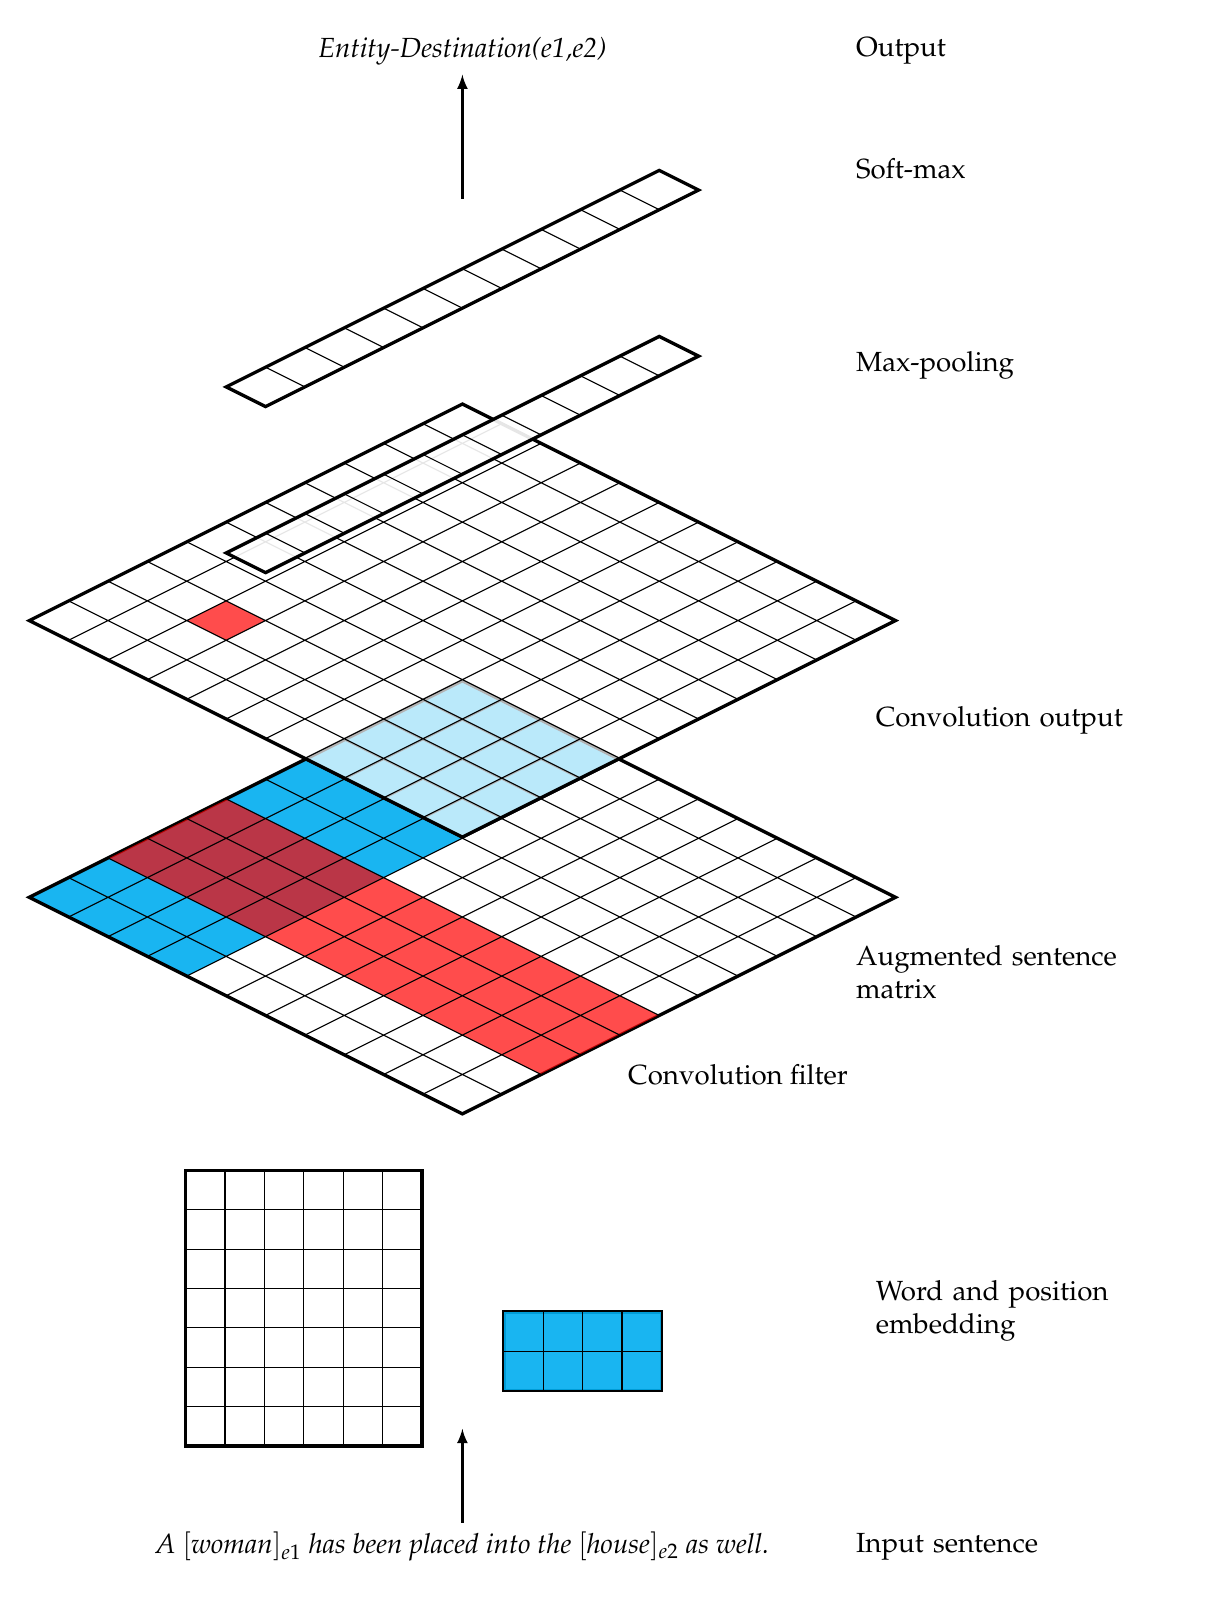
\begin{tikzpicture}[on grid]
    	\begin{scope}[yshift=0,
    				  every node/.append style={
	       	    	  	yslant=0.5,
    	    	        xslant=-1
		    	      },
    	              yslant=0.
    	              5,xslant=-1]
        	\fill[cyan,fill opacity=.9] (0,3.5) rectangle (5.5,5.5);
	        \draw[black,very thick] (0,0) rectangle (5.5,5.5);
	       	\fill[red,fill opacity=.7] (1,0) rectangle (2.5,5.5);
    	    \draw[step=5mm, black] (0,0) grid (5.5,5.5);
    \end{scope}
   	\begin{scope}[yshift=100,
   				  every node/.append style={
   	    	  	    yslant=0.5,
    	    	    xslant=-1
		    	  },
    	          yslant=0.
    	          5,xslant=-1]
        	\fill[white,fill opacity=.7] (0,0) rectangle (5.5,5.5);
        	\fill[red,fill opacity=.7] (1,4.5) rectangle (1.5,4);
	        \draw[black,very thick] (0,0) rectangle (5.5,5.5);
    	    \draw[step=5mm, black] (0,0) grid (5.5,5.5);
    \end{scope}
    \begin{scope}[yshift=160,
    			  xshift=0,
    			  every node/.append style={
	       	      	yslant=0.5,
    	    	    xslant=-1
		    	  },
    	          yslant=0.
    	          5,xslant=-1]
        	\fill[white,fill opacity=.9] (0,3) rectangle (5.5,2.5);
	        \draw[black,very thick] (0,3) rectangle (5.5,2.5);
    	    \draw[step=5mm, black] (0,3) grid (5.5,2.5);
    \end{scope}
    \begin{scope}[yshift=220,
    			  xshift=0,
    			  every node/.append style={
	       	      	yslant=0.5,
    	    	    xslant=-1
		    	  },
    	          yslant=0.
    	          5,xslant=-1]
        	\fill[white,fill opacity=.9] (0,3) rectangle (5.5,2.5);
	        \draw[black,very thick] (0,3) rectangle (5.5,2.5);
    	    \draw[step=5mm, black] (0,3) grid (5.5,2.5);
    \end{scope}
    \begin{scope}[yshift=-120, xshift=-100]
    	\draw[black,very thick] (0,0) rectangle (3,3.5);
   	    \draw[step=5mm, black] (0,0) grid (3,3.5);
    \end{scope}
        \begin{scope}[yshift=-100, xshift=15]
    	\draw[black,very thick] (0,0) rectangle (2,1);
		\fill[cyan,fill opacity=.9] (0,0) rectangle (2,1);
   	    \draw[step=5mm, black] (0,0) grid (2,1);
    \end{scope}
    \node [text width=4cm] at (7,1.8) {Augmented sentence matrix};
    \node [text width=3.5cm] at (7,-2.5) {Word and position embedding};
    \node [text width=4cm] at (7,-5.5) {Input sentence};
    \node [] at (3.5,.5) {Convolution filter};
	\node [text width=3.5cm] at (7,5) {Convolution output};
	\node [text width=4cm] at (7,9.5) {Max-pooling};
	\node [text width=4cm] at (7,12) {Soft-max};
	\node [] (input) at (0,-5.5) {\textit{A $[$woman$]_{e1}$ has been placed into the $[$house$]_{e2}$ as well.}};
	\node [] (output) at (0,13.5) {\textit{Entity-Destination(e1,e2)}};
	\node [text width=4cm] at (7,13.5) {Output};
	\node [] (start) at (0,11.5) {};
	\draw [-latex, thick] (input) edge (0, -4);
	\draw [-latex, thick] (start) edge (output);
	\end{tikzpicture}
	\caption{Diagram of the convolutional neural network for relation classification. The input sentence is mapped to a sentence matrix by concatenating the word-vector for each word in the word embedding matrix and the position-vector for each word-position in the position embedding matrix for both entities. The position embedding components of the architecture is shown in blue. This forms a $K \times d + 2d'$ matrix. Convolution filters are applied along the $K$-axis of the sentence matrix to produce the convolution output. Each element in the convolution output matrix corresponds to one convolution filter applied at one position of the sentence matrix. An example convolutional filter and its corresponding output unit is shown in red. Max-pooling is applied to the convolution output to obtain a feature-vector. This vector is used as input to a soft-max output layer.}
	\label{relation_architecture}
\end{figure}
\FloatBarrier
\newpage

\vspace*{1cm}

\tikzstyle{box} = [rectangle, draw, node distance=3cm, align=center, minimum height=4em, minimum width=18em, thick]
\begin{figure}[h!]
	\centering
	\begin{tikzpicture}
		\node [box] (embedding) at (4,0) {Shared word-embedding matrix};
		\node [box] (position_embedding) at (-4,0) {Shared position-embedding\\matrix};
		\node [box] (convolutions_task1) at (4,4) {Convolutional filters and\\max-pooling};
		\node [box] (convolutions_task2) at (-4,4) {Convolutional filters and\\max-pooling};
		\node [box] (output_1) at (4,8) {Soft-max output};
		\node [box] (output_2) at (-4,8) {Soft-max output};
		\node [box] (aux_sentence) at (4,-4) {Auxiliary task input};
		\node [box] (target_sentence) at (-4,-4) {Target task input};
		\draw[-latex, thick] (target_sentence) edge (embedding);
		\draw[-latex, thick] (target_sentence) edge (position_embedding);
		\draw[-latex, thick, dashed] (aux_sentence) edge (embedding);
		\draw[-latex, thick, dashed] (embedding) edge (convolutions_task1);
		\draw[-latex, thick] (embedding) edge (convolutions_task2);
		\draw[-latex, thick, dashed] (convolutions_task1) edge (output_1);
		\draw[-latex, thick] (convolutions_task2) edge (output_2);
		\draw[-latex, thick] (position_embedding) edge (convolutions_task2);
		\draw[-latex, thick, dashed] (aux_sentence) edge (position_embedding);
		\draw[-latex, thick, dashed] (position_embedding) edge (convolutions_task1);
		
	\end{tikzpicture}
	\caption{Diagram of the weight sharing strategy in which only the embedding matrices are shared between the auxiliary and target task. The solid lines show how network activations flow from the target task to the target output. Dashed lines show how the activations flow through the auxiliary network.}
	\label{relation_sequence_weight_sharing}
\end{figure}
\newpage
\tikzstyle{box} = [rectangle, draw, node distance=3cm, align=center, minimum height=4em, minimum width=18em, thick]
\begin{figure}[h!]
	\centering
	\begin{tikzpicture}
		\node [box] (embedding) at (4,0) {Shared word-embedding matrix};
		\node [box] (position_embedding) at (-4,0) {Shared position-embedding\\matrix};
		\node [box] (convolutions_task1) at (4,4) {Shared convolutional filters and\\max-pooling};
		\node [box] (convolutions_task2) at (-4,4) {Convolutional filters and\\max-pooling};
		\node [box] (output_1) at (4,8) {Soft-max output};
		\node [box] (output_2) at (-4,8) {Soft-max output};
		\node [box] (aux_sentence) at (4,-4) {Auxiliary task input};
		\node [box] (target_sentence) at (-4,-4) {Target task input};
		\draw[-latex, thick] (target_sentence) edge (embedding);
		\draw[-latex, thick] (convolutions_task1) edge (output_2);
		\draw[-latex, thick] (target_sentence) edge (position_embedding);
		\draw[-latex, thick, dashed] (aux_sentence) edge (embedding);
		\draw[-latex, thick, dashed, transform canvas={xshift=.8cm}] (embedding) edge (convolutions_task1);
		\draw[-latex, thick, transform canvas={xshift=-.8cm}] (embedding) edge (convolutions_task1);
		\draw[-latex, thick] (embedding) edge (convolutions_task2);
		\draw[-latex, thick, dashed] (convolutions_task1) edge (output_1);
		\draw[-latex, thick] (convolutions_task2) edge (output_2);
		\draw[-latex, thick] (position_embedding) edge (convolutions_task2);
		\draw[-latex, thick, dashed] (aux_sentence) edge (position_embedding);
		\draw[-latex, thick, dashed] (position_embedding) edge (convolutions_task1);
		
	\end{tikzpicture}
	\caption{Diagram of how neural network weights are shared when using a multi channel convolutional network to enable sharing convolutional filters. The solid lines show how network activations flow from the target task to the target output. Dashed lines show how the activations flow through the auxiliary network.}
\end{figure}
\FloatBarrier

\chapter{Results}
In this section we present the results obtained in the experiment detailed in the previous sections. We visualize the effect of multi-task learning on generalization error estimated by cross-validation for each of the proposed weight sharing strategies. Specifically, we plot the mean macro F1 for each cross-validation experiment as a function of the fraction of target data available for training. This produces a so called \textbf{learning curve} that indicates how generalization error improves as the amount of training data is increased in both the single-task and multi-task setting.
\\\\
Moreover, we perform statistical tests of significance using one sided t-testing on the data collected for each fraction $f$ of target data in order to determine if the observed differences between single-task and multi-task learning can be explained by variation due to random weight initialization and and stochastic gradient descent.
\newpage
\section{Shared Embeddings}
\newpage
\section{Shared Side Channel Convolutional Filters}
In this section we present the results obtained for SemEval 2010 Task 8 in a single-task and multi-task setting using the multi-channel weight sharing strategy discussed in section \ref{network_architecture}. Each plot contains two curves: one learning curve for SemEval 2010 Task 8 when learnt as a single task, and one when learnt simultaneously with an auxiliary task. In addition we present tables containing the $p$-value of one-sided t-tests between the macro $F1$ scores of multi-task and single-task experiments grouped by the fraction of target data $f$.
\vspace{2cm}
\begin{figure}[h]
	\centering
	%% Creator: Matplotlib, PGF backend
%%
%% To include the figure in your LaTeX document, write
%%   \input{<filename>.pgf}
%%
%% Make sure the required packages are loaded in your preamble
%%   \usepackage{pgf}
%%
%% Figures using additional raster images can only be included by \input if
%% they are in the same directory as the main LaTeX file. For loading figures
%% from other directories you can use the `import` package
%%   \usepackage{import}
%% and then include the figures with
%%   \import{<path to file>}{<filename>.pgf}
%%
%% Matplotlib used the following preamble
%%   \usepackage{fontspec}
%%   \setmainfont{Palatino}
%%   \setsansfont{Lucida Grande}
%%   \setmonofont{Andale Mono}
%%
\begingroup%
\makeatletter%
\begin{pgfpicture}%
\pgfpathrectangle{\pgfpointorigin}{\pgfqpoint{5.004722in}{3.175278in}}%
\pgfusepath{use as bounding box, clip}%
\begin{pgfscope}%
\pgfsetbuttcap%
\pgfsetmiterjoin%
\definecolor{currentfill}{rgb}{1.000000,1.000000,1.000000}%
\pgfsetfillcolor{currentfill}%
\pgfsetlinewidth{0.000000pt}%
\definecolor{currentstroke}{rgb}{1.000000,1.000000,1.000000}%
\pgfsetstrokecolor{currentstroke}%
\pgfsetdash{}{0pt}%
\pgfpathmoveto{\pgfqpoint{0.000000in}{0.000000in}}%
\pgfpathlineto{\pgfqpoint{5.004722in}{0.000000in}}%
\pgfpathlineto{\pgfqpoint{5.004722in}{3.175278in}}%
\pgfpathlineto{\pgfqpoint{0.000000in}{3.175278in}}%
\pgfpathclose%
\pgfusepath{fill}%
\end{pgfscope}%
\begin{pgfscope}%
\pgfsetbuttcap%
\pgfsetmiterjoin%
\definecolor{currentfill}{rgb}{1.000000,1.000000,1.000000}%
\pgfsetfillcolor{currentfill}%
\pgfsetlinewidth{0.000000pt}%
\definecolor{currentstroke}{rgb}{0.000000,0.000000,0.000000}%
\pgfsetstrokecolor{currentstroke}%
\pgfsetstrokeopacity{0.000000}%
\pgfsetdash{}{0pt}%
\pgfpathmoveto{\pgfqpoint{0.430962in}{0.403645in}}%
\pgfpathlineto{\pgfqpoint{4.916179in}{0.403645in}}%
\pgfpathlineto{\pgfqpoint{4.916179in}{3.157778in}}%
\pgfpathlineto{\pgfqpoint{0.430962in}{3.157778in}}%
\pgfpathclose%
\pgfusepath{fill}%
\end{pgfscope}%
\begin{pgfscope}%
\pgfsetbuttcap%
\pgfsetroundjoin%
\definecolor{currentfill}{rgb}{0.000000,0.000000,0.000000}%
\pgfsetfillcolor{currentfill}%
\pgfsetlinewidth{0.803000pt}%
\definecolor{currentstroke}{rgb}{0.000000,0.000000,0.000000}%
\pgfsetstrokecolor{currentstroke}%
\pgfsetdash{}{0pt}%
\pgfsys@defobject{currentmarker}{\pgfqpoint{0.000000in}{-0.048611in}}{\pgfqpoint{0.000000in}{0.000000in}}{%
\pgfpathmoveto{\pgfqpoint{0.000000in}{0.000000in}}%
\pgfpathlineto{\pgfqpoint{0.000000in}{-0.048611in}}%
\pgfusepath{stroke,fill}%
}%
\begin{pgfscope}%
\pgfsys@transformshift{0.430962in}{0.403645in}%
\pgfsys@useobject{currentmarker}{}%
\end{pgfscope}%
\end{pgfscope}%
\begin{pgfscope}%
\pgftext[x=0.430962in,y=0.306423in,,top]{\rmfamily\fontsize{8.000000}{9.600000}\selectfont \(\displaystyle 0\)}%
\end{pgfscope}%
\begin{pgfscope}%
\pgfsetbuttcap%
\pgfsetroundjoin%
\definecolor{currentfill}{rgb}{0.000000,0.000000,0.000000}%
\pgfsetfillcolor{currentfill}%
\pgfsetlinewidth{0.803000pt}%
\definecolor{currentstroke}{rgb}{0.000000,0.000000,0.000000}%
\pgfsetstrokecolor{currentstroke}%
\pgfsetdash{}{0pt}%
\pgfsys@defobject{currentmarker}{\pgfqpoint{0.000000in}{-0.048611in}}{\pgfqpoint{0.000000in}{0.000000in}}{%
\pgfpathmoveto{\pgfqpoint{0.000000in}{0.000000in}}%
\pgfpathlineto{\pgfqpoint{0.000000in}{-0.048611in}}%
\pgfusepath{stroke,fill}%
}%
\begin{pgfscope}%
\pgfsys@transformshift{1.328006in}{0.403645in}%
\pgfsys@useobject{currentmarker}{}%
\end{pgfscope}%
\end{pgfscope}%
\begin{pgfscope}%
\pgftext[x=1.328006in,y=0.306423in,,top]{\rmfamily\fontsize{8.000000}{9.600000}\selectfont \(\displaystyle 20\)}%
\end{pgfscope}%
\begin{pgfscope}%
\pgfsetbuttcap%
\pgfsetroundjoin%
\definecolor{currentfill}{rgb}{0.000000,0.000000,0.000000}%
\pgfsetfillcolor{currentfill}%
\pgfsetlinewidth{0.803000pt}%
\definecolor{currentstroke}{rgb}{0.000000,0.000000,0.000000}%
\pgfsetstrokecolor{currentstroke}%
\pgfsetdash{}{0pt}%
\pgfsys@defobject{currentmarker}{\pgfqpoint{0.000000in}{-0.048611in}}{\pgfqpoint{0.000000in}{0.000000in}}{%
\pgfpathmoveto{\pgfqpoint{0.000000in}{0.000000in}}%
\pgfpathlineto{\pgfqpoint{0.000000in}{-0.048611in}}%
\pgfusepath{stroke,fill}%
}%
\begin{pgfscope}%
\pgfsys@transformshift{2.225049in}{0.403645in}%
\pgfsys@useobject{currentmarker}{}%
\end{pgfscope}%
\end{pgfscope}%
\begin{pgfscope}%
\pgftext[x=2.225049in,y=0.306423in,,top]{\rmfamily\fontsize{8.000000}{9.600000}\selectfont \(\displaystyle 40\)}%
\end{pgfscope}%
\begin{pgfscope}%
\pgfsetbuttcap%
\pgfsetroundjoin%
\definecolor{currentfill}{rgb}{0.000000,0.000000,0.000000}%
\pgfsetfillcolor{currentfill}%
\pgfsetlinewidth{0.803000pt}%
\definecolor{currentstroke}{rgb}{0.000000,0.000000,0.000000}%
\pgfsetstrokecolor{currentstroke}%
\pgfsetdash{}{0pt}%
\pgfsys@defobject{currentmarker}{\pgfqpoint{0.000000in}{-0.048611in}}{\pgfqpoint{0.000000in}{0.000000in}}{%
\pgfpathmoveto{\pgfqpoint{0.000000in}{0.000000in}}%
\pgfpathlineto{\pgfqpoint{0.000000in}{-0.048611in}}%
\pgfusepath{stroke,fill}%
}%
\begin{pgfscope}%
\pgfsys@transformshift{3.122092in}{0.403645in}%
\pgfsys@useobject{currentmarker}{}%
\end{pgfscope}%
\end{pgfscope}%
\begin{pgfscope}%
\pgftext[x=3.122092in,y=0.306423in,,top]{\rmfamily\fontsize{8.000000}{9.600000}\selectfont \(\displaystyle 60\)}%
\end{pgfscope}%
\begin{pgfscope}%
\pgfsetbuttcap%
\pgfsetroundjoin%
\definecolor{currentfill}{rgb}{0.000000,0.000000,0.000000}%
\pgfsetfillcolor{currentfill}%
\pgfsetlinewidth{0.803000pt}%
\definecolor{currentstroke}{rgb}{0.000000,0.000000,0.000000}%
\pgfsetstrokecolor{currentstroke}%
\pgfsetdash{}{0pt}%
\pgfsys@defobject{currentmarker}{\pgfqpoint{0.000000in}{-0.048611in}}{\pgfqpoint{0.000000in}{0.000000in}}{%
\pgfpathmoveto{\pgfqpoint{0.000000in}{0.000000in}}%
\pgfpathlineto{\pgfqpoint{0.000000in}{-0.048611in}}%
\pgfusepath{stroke,fill}%
}%
\begin{pgfscope}%
\pgfsys@transformshift{4.019135in}{0.403645in}%
\pgfsys@useobject{currentmarker}{}%
\end{pgfscope}%
\end{pgfscope}%
\begin{pgfscope}%
\pgftext[x=4.019135in,y=0.306423in,,top]{\rmfamily\fontsize{8.000000}{9.600000}\selectfont \(\displaystyle 80\)}%
\end{pgfscope}%
\begin{pgfscope}%
\pgfsetbuttcap%
\pgfsetroundjoin%
\definecolor{currentfill}{rgb}{0.000000,0.000000,0.000000}%
\pgfsetfillcolor{currentfill}%
\pgfsetlinewidth{0.803000pt}%
\definecolor{currentstroke}{rgb}{0.000000,0.000000,0.000000}%
\pgfsetstrokecolor{currentstroke}%
\pgfsetdash{}{0pt}%
\pgfsys@defobject{currentmarker}{\pgfqpoint{0.000000in}{-0.048611in}}{\pgfqpoint{0.000000in}{0.000000in}}{%
\pgfpathmoveto{\pgfqpoint{0.000000in}{0.000000in}}%
\pgfpathlineto{\pgfqpoint{0.000000in}{-0.048611in}}%
\pgfusepath{stroke,fill}%
}%
\begin{pgfscope}%
\pgfsys@transformshift{4.916179in}{0.403645in}%
\pgfsys@useobject{currentmarker}{}%
\end{pgfscope}%
\end{pgfscope}%
\begin{pgfscope}%
\pgftext[x=4.916179in,y=0.306423in,,top]{\rmfamily\fontsize{8.000000}{9.600000}\selectfont \(\displaystyle 100\)}%
\end{pgfscope}%
\begin{pgfscope}%
\pgftext[x=2.673571in,y=0.139431in,,top]{\rmfamily\fontsize{10.000000}{12.000000}\selectfont percentage of \(\displaystyle \mathcal{D}_t\)}%
\end{pgfscope}%
\begin{pgfscope}%
\pgfsetbuttcap%
\pgfsetroundjoin%
\definecolor{currentfill}{rgb}{0.000000,0.000000,0.000000}%
\pgfsetfillcolor{currentfill}%
\pgfsetlinewidth{0.803000pt}%
\definecolor{currentstroke}{rgb}{0.000000,0.000000,0.000000}%
\pgfsetstrokecolor{currentstroke}%
\pgfsetdash{}{0pt}%
\pgfsys@defobject{currentmarker}{\pgfqpoint{-0.048611in}{0.000000in}}{\pgfqpoint{0.000000in}{0.000000in}}{%
\pgfpathmoveto{\pgfqpoint{0.000000in}{0.000000in}}%
\pgfpathlineto{\pgfqpoint{-0.048611in}{0.000000in}}%
\pgfusepath{stroke,fill}%
}%
\begin{pgfscope}%
\pgfsys@transformshift{0.430962in}{0.702564in}%
\pgfsys@useobject{currentmarker}{}%
\end{pgfscope}%
\end{pgfscope}%
\begin{pgfscope}%
\pgftext[x=0.194851in,y=0.662145in,left,base]{\rmfamily\fontsize{8.000000}{9.600000}\selectfont 0.1}%
\end{pgfscope}%
\begin{pgfscope}%
\pgfsetbuttcap%
\pgfsetroundjoin%
\definecolor{currentfill}{rgb}{0.000000,0.000000,0.000000}%
\pgfsetfillcolor{currentfill}%
\pgfsetlinewidth{0.803000pt}%
\definecolor{currentstroke}{rgb}{0.000000,0.000000,0.000000}%
\pgfsetstrokecolor{currentstroke}%
\pgfsetdash{}{0pt}%
\pgfsys@defobject{currentmarker}{\pgfqpoint{-0.048611in}{0.000000in}}{\pgfqpoint{0.000000in}{0.000000in}}{%
\pgfpathmoveto{\pgfqpoint{0.000000in}{0.000000in}}%
\pgfpathlineto{\pgfqpoint{-0.048611in}{0.000000in}}%
\pgfusepath{stroke,fill}%
}%
\begin{pgfscope}%
\pgfsys@transformshift{0.430962in}{1.095135in}%
\pgfsys@useobject{currentmarker}{}%
\end{pgfscope}%
\end{pgfscope}%
\begin{pgfscope}%
\pgftext[x=0.194851in,y=1.054716in,left,base]{\rmfamily\fontsize{8.000000}{9.600000}\selectfont 0.2}%
\end{pgfscope}%
\begin{pgfscope}%
\pgfsetbuttcap%
\pgfsetroundjoin%
\definecolor{currentfill}{rgb}{0.000000,0.000000,0.000000}%
\pgfsetfillcolor{currentfill}%
\pgfsetlinewidth{0.803000pt}%
\definecolor{currentstroke}{rgb}{0.000000,0.000000,0.000000}%
\pgfsetstrokecolor{currentstroke}%
\pgfsetdash{}{0pt}%
\pgfsys@defobject{currentmarker}{\pgfqpoint{-0.048611in}{0.000000in}}{\pgfqpoint{0.000000in}{0.000000in}}{%
\pgfpathmoveto{\pgfqpoint{0.000000in}{0.000000in}}%
\pgfpathlineto{\pgfqpoint{-0.048611in}{0.000000in}}%
\pgfusepath{stroke,fill}%
}%
\begin{pgfscope}%
\pgfsys@transformshift{0.430962in}{1.487706in}%
\pgfsys@useobject{currentmarker}{}%
\end{pgfscope}%
\end{pgfscope}%
\begin{pgfscope}%
\pgftext[x=0.194851in,y=1.447287in,left,base]{\rmfamily\fontsize{8.000000}{9.600000}\selectfont 0.3}%
\end{pgfscope}%
\begin{pgfscope}%
\pgfsetbuttcap%
\pgfsetroundjoin%
\definecolor{currentfill}{rgb}{0.000000,0.000000,0.000000}%
\pgfsetfillcolor{currentfill}%
\pgfsetlinewidth{0.803000pt}%
\definecolor{currentstroke}{rgb}{0.000000,0.000000,0.000000}%
\pgfsetstrokecolor{currentstroke}%
\pgfsetdash{}{0pt}%
\pgfsys@defobject{currentmarker}{\pgfqpoint{-0.048611in}{0.000000in}}{\pgfqpoint{0.000000in}{0.000000in}}{%
\pgfpathmoveto{\pgfqpoint{0.000000in}{0.000000in}}%
\pgfpathlineto{\pgfqpoint{-0.048611in}{0.000000in}}%
\pgfusepath{stroke,fill}%
}%
\begin{pgfscope}%
\pgfsys@transformshift{0.430962in}{1.880276in}%
\pgfsys@useobject{currentmarker}{}%
\end{pgfscope}%
\end{pgfscope}%
\begin{pgfscope}%
\pgftext[x=0.194851in,y=1.839858in,left,base]{\rmfamily\fontsize{8.000000}{9.600000}\selectfont 0.4}%
\end{pgfscope}%
\begin{pgfscope}%
\pgfsetbuttcap%
\pgfsetroundjoin%
\definecolor{currentfill}{rgb}{0.000000,0.000000,0.000000}%
\pgfsetfillcolor{currentfill}%
\pgfsetlinewidth{0.803000pt}%
\definecolor{currentstroke}{rgb}{0.000000,0.000000,0.000000}%
\pgfsetstrokecolor{currentstroke}%
\pgfsetdash{}{0pt}%
\pgfsys@defobject{currentmarker}{\pgfqpoint{-0.048611in}{0.000000in}}{\pgfqpoint{0.000000in}{0.000000in}}{%
\pgfpathmoveto{\pgfqpoint{0.000000in}{0.000000in}}%
\pgfpathlineto{\pgfqpoint{-0.048611in}{0.000000in}}%
\pgfusepath{stroke,fill}%
}%
\begin{pgfscope}%
\pgfsys@transformshift{0.430962in}{2.272847in}%
\pgfsys@useobject{currentmarker}{}%
\end{pgfscope}%
\end{pgfscope}%
\begin{pgfscope}%
\pgftext[x=0.194851in,y=2.232429in,left,base]{\rmfamily\fontsize{8.000000}{9.600000}\selectfont 0.5}%
\end{pgfscope}%
\begin{pgfscope}%
\pgfsetbuttcap%
\pgfsetroundjoin%
\definecolor{currentfill}{rgb}{0.000000,0.000000,0.000000}%
\pgfsetfillcolor{currentfill}%
\pgfsetlinewidth{0.803000pt}%
\definecolor{currentstroke}{rgb}{0.000000,0.000000,0.000000}%
\pgfsetstrokecolor{currentstroke}%
\pgfsetdash{}{0pt}%
\pgfsys@defobject{currentmarker}{\pgfqpoint{-0.048611in}{0.000000in}}{\pgfqpoint{0.000000in}{0.000000in}}{%
\pgfpathmoveto{\pgfqpoint{0.000000in}{0.000000in}}%
\pgfpathlineto{\pgfqpoint{-0.048611in}{0.000000in}}%
\pgfusepath{stroke,fill}%
}%
\begin{pgfscope}%
\pgfsys@transformshift{0.430962in}{2.665418in}%
\pgfsys@useobject{currentmarker}{}%
\end{pgfscope}%
\end{pgfscope}%
\begin{pgfscope}%
\pgftext[x=0.194851in,y=2.624999in,left,base]{\rmfamily\fontsize{8.000000}{9.600000}\selectfont 0.6}%
\end{pgfscope}%
\begin{pgfscope}%
\pgfsetbuttcap%
\pgfsetroundjoin%
\definecolor{currentfill}{rgb}{0.000000,0.000000,0.000000}%
\pgfsetfillcolor{currentfill}%
\pgfsetlinewidth{0.803000pt}%
\definecolor{currentstroke}{rgb}{0.000000,0.000000,0.000000}%
\pgfsetstrokecolor{currentstroke}%
\pgfsetdash{}{0pt}%
\pgfsys@defobject{currentmarker}{\pgfqpoint{-0.048611in}{0.000000in}}{\pgfqpoint{0.000000in}{0.000000in}}{%
\pgfpathmoveto{\pgfqpoint{0.000000in}{0.000000in}}%
\pgfpathlineto{\pgfqpoint{-0.048611in}{0.000000in}}%
\pgfusepath{stroke,fill}%
}%
\begin{pgfscope}%
\pgfsys@transformshift{0.430962in}{3.057989in}%
\pgfsys@useobject{currentmarker}{}%
\end{pgfscope}%
\end{pgfscope}%
\begin{pgfscope}%
\pgftext[x=0.194851in,y=3.017570in,left,base]{\rmfamily\fontsize{8.000000}{9.600000}\selectfont 0.7}%
\end{pgfscope}%
\begin{pgfscope}%
\pgftext[x=0.139296in,y=1.780712in,,bottom,rotate=90.000000]{\rmfamily\fontsize{10.000000}{12.000000}\selectfont Mean macro F1}%
\end{pgfscope}%
\begin{pgfscope}%
\pgfpathrectangle{\pgfqpoint{0.430962in}{0.403645in}}{\pgfqpoint{4.485217in}{2.754132in}} %
\pgfusepath{clip}%
\pgfsetrectcap%
\pgfsetroundjoin%
\pgfsetlinewidth{1.505625pt}%
\definecolor{currentstroke}{rgb}{0.121569,0.466667,0.705882}%
\pgfsetstrokecolor{currentstroke}%
\pgfsetdash{}{0pt}%
\pgfpathmoveto{\pgfqpoint{0.430962in}{0.528833in}}%
\pgfpathlineto{\pgfqpoint{1.328006in}{2.690585in}}%
\pgfpathlineto{\pgfqpoint{2.225049in}{2.870213in}}%
\pgfpathlineto{\pgfqpoint{3.122092in}{2.927016in}}%
\pgfpathlineto{\pgfqpoint{4.019135in}{2.946813in}}%
\pgfpathlineto{\pgfqpoint{4.916179in}{2.989337in}}%
\pgfusepath{stroke}%
\end{pgfscope}%
\begin{pgfscope}%
\pgfpathrectangle{\pgfqpoint{0.430962in}{0.403645in}}{\pgfqpoint{4.485217in}{2.754132in}} %
\pgfusepath{clip}%
\pgfsetbuttcap%
\pgfsetroundjoin%
\pgfsetlinewidth{1.505625pt}%
\definecolor{currentstroke}{rgb}{1.000000,0.498039,0.054902}%
\pgfsetstrokecolor{currentstroke}%
\pgfsetdash{{5.550000pt}{2.400000pt}}{0.000000pt}%
\pgfpathmoveto{\pgfqpoint{0.430962in}{0.537862in}}%
\pgfpathlineto{\pgfqpoint{1.328006in}{2.710362in}}%
\pgfpathlineto{\pgfqpoint{2.225049in}{2.883755in}}%
\pgfpathlineto{\pgfqpoint{3.122092in}{2.983473in}}%
\pgfpathlineto{\pgfqpoint{4.019135in}{3.032590in}}%
\pgfpathlineto{\pgfqpoint{4.916179in}{3.001802in}}%
\pgfusepath{stroke}%
\end{pgfscope}%
\begin{pgfscope}%
\pgfsetrectcap%
\pgfsetmiterjoin%
\pgfsetlinewidth{0.501875pt}%
\definecolor{currentstroke}{rgb}{0.000000,0.000000,0.000000}%
\pgfsetstrokecolor{currentstroke}%
\pgfsetdash{}{0pt}%
\pgfpathmoveto{\pgfqpoint{0.430962in}{0.403645in}}%
\pgfpathlineto{\pgfqpoint{0.430962in}{3.157778in}}%
\pgfusepath{stroke}%
\end{pgfscope}%
\begin{pgfscope}%
\pgfsetrectcap%
\pgfsetmiterjoin%
\pgfsetlinewidth{0.501875pt}%
\definecolor{currentstroke}{rgb}{0.000000,0.000000,0.000000}%
\pgfsetstrokecolor{currentstroke}%
\pgfsetdash{}{0pt}%
\pgfpathmoveto{\pgfqpoint{0.430962in}{0.403645in}}%
\pgfpathlineto{\pgfqpoint{4.916179in}{0.403645in}}%
\pgfusepath{stroke}%
\end{pgfscope}%
\begin{pgfscope}%
\pgfsetrectcap%
\pgfsetroundjoin%
\pgfsetlinewidth{1.505625pt}%
\definecolor{currentstroke}{rgb}{0.121569,0.466667,0.705882}%
\pgfsetstrokecolor{currentstroke}%
\pgfsetdash{}{0pt}%
\pgfpathmoveto{\pgfqpoint{3.315617in}{0.782185in}}%
\pgfpathlineto{\pgfqpoint{3.565617in}{0.782185in}}%
\pgfusepath{stroke}%
\end{pgfscope}%
\begin{pgfscope}%
\pgftext[x=3.665617in,y=0.738435in,left,base]{\rmfamily\fontsize{9.000000}{10.800000}\selectfont SemEval 2010 Task 8}%
\end{pgfscope}%
\begin{pgfscope}%
\pgfsetbuttcap%
\pgfsetroundjoin%
\pgfsetlinewidth{1.505625pt}%
\definecolor{currentstroke}{rgb}{1.000000,0.498039,0.054902}%
\pgfsetstrokecolor{currentstroke}%
\pgfsetdash{{5.550000pt}{2.400000pt}}{0.000000pt}%
\pgfpathmoveto{\pgfqpoint{3.315617in}{0.594319in}}%
\pgfpathlineto{\pgfqpoint{3.565617in}{0.594319in}}%
\pgfusepath{stroke}%
\end{pgfscope}%
\begin{pgfscope}%
\pgftext[x=3.665617in,y=0.550569in,left,base]{\rmfamily\fontsize{9.000000}{10.800000}\selectfont +ACE 2005}%
\end{pgfscope}%
\end{pgfpicture}%
\makeatother%
\endgroup%

	
	\vspace*{1cm}
	
	\begin{tabular}{r | l | l | l | l | l | l}
		\textbf{Percentage of $\data_t$} & 0 & 20 & 40 & 60 & 80 & 100 \\  \hline
		\textbf{Mean single-task macro $F1$} & .056 & .606 & .652 & .667 & .672 & .683\\
		\textbf{Mean multi-task macro $F1$} & 0 & 0 & 0 & 0 & 0 & 0\\
		$p$\textbf{-value} & 0 & 0 & 0 & 0 & 0 & 0
	\end{tabular}
	\caption{Learning curves and hypothesis tests for SemEval 2010 Task 8 trained as a single task and in a multi-task setting with ACE 2005. The learning curves indicate a slight improvement of multi-task learning over single-task learning in the 60-80\% range}
\end{figure}
\begin{figure}
	\centering
	%% Creator: Matplotlib, PGF backend
%%
%% To include the figure in your LaTeX document, write
%%   \input{<filename>.pgf}
%%
%% Make sure the required packages are loaded in your preamble
%%   \usepackage{pgf}
%%
%% Figures using additional raster images can only be included by \input if
%% they are in the same directory as the main LaTeX file. For loading figures
%% from other directories you can use the `import` package
%%   \usepackage{import}
%% and then include the figures with
%%   \import{<path to file>}{<filename>.pgf}
%%
%% Matplotlib used the following preamble
%%   \usepackage{fontspec}
%%   \setmainfont{Palatino}
%%   \setsansfont{Lucida Grande}
%%   \setmonofont{Andale Mono}
%%
\begingroup%
\makeatletter%
\begin{pgfpicture}%
\pgfpathrectangle{\pgfpointorigin}{\pgfqpoint{5.004722in}{3.175278in}}%
\pgfusepath{use as bounding box, clip}%
\begin{pgfscope}%
\pgfsetbuttcap%
\pgfsetmiterjoin%
\definecolor{currentfill}{rgb}{1.000000,1.000000,1.000000}%
\pgfsetfillcolor{currentfill}%
\pgfsetlinewidth{0.000000pt}%
\definecolor{currentstroke}{rgb}{1.000000,1.000000,1.000000}%
\pgfsetstrokecolor{currentstroke}%
\pgfsetdash{}{0pt}%
\pgfpathmoveto{\pgfqpoint{0.000000in}{0.000000in}}%
\pgfpathlineto{\pgfqpoint{5.004722in}{0.000000in}}%
\pgfpathlineto{\pgfqpoint{5.004722in}{3.175278in}}%
\pgfpathlineto{\pgfqpoint{0.000000in}{3.175278in}}%
\pgfpathclose%
\pgfusepath{fill}%
\end{pgfscope}%
\begin{pgfscope}%
\pgfsetbuttcap%
\pgfsetmiterjoin%
\definecolor{currentfill}{rgb}{1.000000,1.000000,1.000000}%
\pgfsetfillcolor{currentfill}%
\pgfsetlinewidth{0.000000pt}%
\definecolor{currentstroke}{rgb}{0.000000,0.000000,0.000000}%
\pgfsetstrokecolor{currentstroke}%
\pgfsetstrokeopacity{0.000000}%
\pgfsetdash{}{0pt}%
\pgfpathmoveto{\pgfqpoint{0.430962in}{0.403645in}}%
\pgfpathlineto{\pgfqpoint{4.916179in}{0.403645in}}%
\pgfpathlineto{\pgfqpoint{4.916179in}{3.157778in}}%
\pgfpathlineto{\pgfqpoint{0.430962in}{3.157778in}}%
\pgfpathclose%
\pgfusepath{fill}%
\end{pgfscope}%
\begin{pgfscope}%
\pgfsetbuttcap%
\pgfsetroundjoin%
\definecolor{currentfill}{rgb}{0.000000,0.000000,0.000000}%
\pgfsetfillcolor{currentfill}%
\pgfsetlinewidth{0.803000pt}%
\definecolor{currentstroke}{rgb}{0.000000,0.000000,0.000000}%
\pgfsetstrokecolor{currentstroke}%
\pgfsetdash{}{0pt}%
\pgfsys@defobject{currentmarker}{\pgfqpoint{0.000000in}{-0.048611in}}{\pgfqpoint{0.000000in}{0.000000in}}{%
\pgfpathmoveto{\pgfqpoint{0.000000in}{0.000000in}}%
\pgfpathlineto{\pgfqpoint{0.000000in}{-0.048611in}}%
\pgfusepath{stroke,fill}%
}%
\begin{pgfscope}%
\pgfsys@transformshift{0.430962in}{0.403645in}%
\pgfsys@useobject{currentmarker}{}%
\end{pgfscope}%
\end{pgfscope}%
\begin{pgfscope}%
\pgftext[x=0.430962in,y=0.306423in,,top]{\rmfamily\fontsize{8.000000}{9.600000}\selectfont \(\displaystyle 0\)}%
\end{pgfscope}%
\begin{pgfscope}%
\pgfsetbuttcap%
\pgfsetroundjoin%
\definecolor{currentfill}{rgb}{0.000000,0.000000,0.000000}%
\pgfsetfillcolor{currentfill}%
\pgfsetlinewidth{0.803000pt}%
\definecolor{currentstroke}{rgb}{0.000000,0.000000,0.000000}%
\pgfsetstrokecolor{currentstroke}%
\pgfsetdash{}{0pt}%
\pgfsys@defobject{currentmarker}{\pgfqpoint{0.000000in}{-0.048611in}}{\pgfqpoint{0.000000in}{0.000000in}}{%
\pgfpathmoveto{\pgfqpoint{0.000000in}{0.000000in}}%
\pgfpathlineto{\pgfqpoint{0.000000in}{-0.048611in}}%
\pgfusepath{stroke,fill}%
}%
\begin{pgfscope}%
\pgfsys@transformshift{1.328006in}{0.403645in}%
\pgfsys@useobject{currentmarker}{}%
\end{pgfscope}%
\end{pgfscope}%
\begin{pgfscope}%
\pgftext[x=1.328006in,y=0.306423in,,top]{\rmfamily\fontsize{8.000000}{9.600000}\selectfont \(\displaystyle 20\)}%
\end{pgfscope}%
\begin{pgfscope}%
\pgfsetbuttcap%
\pgfsetroundjoin%
\definecolor{currentfill}{rgb}{0.000000,0.000000,0.000000}%
\pgfsetfillcolor{currentfill}%
\pgfsetlinewidth{0.803000pt}%
\definecolor{currentstroke}{rgb}{0.000000,0.000000,0.000000}%
\pgfsetstrokecolor{currentstroke}%
\pgfsetdash{}{0pt}%
\pgfsys@defobject{currentmarker}{\pgfqpoint{0.000000in}{-0.048611in}}{\pgfqpoint{0.000000in}{0.000000in}}{%
\pgfpathmoveto{\pgfqpoint{0.000000in}{0.000000in}}%
\pgfpathlineto{\pgfqpoint{0.000000in}{-0.048611in}}%
\pgfusepath{stroke,fill}%
}%
\begin{pgfscope}%
\pgfsys@transformshift{2.225049in}{0.403645in}%
\pgfsys@useobject{currentmarker}{}%
\end{pgfscope}%
\end{pgfscope}%
\begin{pgfscope}%
\pgftext[x=2.225049in,y=0.306423in,,top]{\rmfamily\fontsize{8.000000}{9.600000}\selectfont \(\displaystyle 40\)}%
\end{pgfscope}%
\begin{pgfscope}%
\pgfsetbuttcap%
\pgfsetroundjoin%
\definecolor{currentfill}{rgb}{0.000000,0.000000,0.000000}%
\pgfsetfillcolor{currentfill}%
\pgfsetlinewidth{0.803000pt}%
\definecolor{currentstroke}{rgb}{0.000000,0.000000,0.000000}%
\pgfsetstrokecolor{currentstroke}%
\pgfsetdash{}{0pt}%
\pgfsys@defobject{currentmarker}{\pgfqpoint{0.000000in}{-0.048611in}}{\pgfqpoint{0.000000in}{0.000000in}}{%
\pgfpathmoveto{\pgfqpoint{0.000000in}{0.000000in}}%
\pgfpathlineto{\pgfqpoint{0.000000in}{-0.048611in}}%
\pgfusepath{stroke,fill}%
}%
\begin{pgfscope}%
\pgfsys@transformshift{3.122092in}{0.403645in}%
\pgfsys@useobject{currentmarker}{}%
\end{pgfscope}%
\end{pgfscope}%
\begin{pgfscope}%
\pgftext[x=3.122092in,y=0.306423in,,top]{\rmfamily\fontsize{8.000000}{9.600000}\selectfont \(\displaystyle 60\)}%
\end{pgfscope}%
\begin{pgfscope}%
\pgfsetbuttcap%
\pgfsetroundjoin%
\definecolor{currentfill}{rgb}{0.000000,0.000000,0.000000}%
\pgfsetfillcolor{currentfill}%
\pgfsetlinewidth{0.803000pt}%
\definecolor{currentstroke}{rgb}{0.000000,0.000000,0.000000}%
\pgfsetstrokecolor{currentstroke}%
\pgfsetdash{}{0pt}%
\pgfsys@defobject{currentmarker}{\pgfqpoint{0.000000in}{-0.048611in}}{\pgfqpoint{0.000000in}{0.000000in}}{%
\pgfpathmoveto{\pgfqpoint{0.000000in}{0.000000in}}%
\pgfpathlineto{\pgfqpoint{0.000000in}{-0.048611in}}%
\pgfusepath{stroke,fill}%
}%
\begin{pgfscope}%
\pgfsys@transformshift{4.019135in}{0.403645in}%
\pgfsys@useobject{currentmarker}{}%
\end{pgfscope}%
\end{pgfscope}%
\begin{pgfscope}%
\pgftext[x=4.019135in,y=0.306423in,,top]{\rmfamily\fontsize{8.000000}{9.600000}\selectfont \(\displaystyle 80\)}%
\end{pgfscope}%
\begin{pgfscope}%
\pgfsetbuttcap%
\pgfsetroundjoin%
\definecolor{currentfill}{rgb}{0.000000,0.000000,0.000000}%
\pgfsetfillcolor{currentfill}%
\pgfsetlinewidth{0.803000pt}%
\definecolor{currentstroke}{rgb}{0.000000,0.000000,0.000000}%
\pgfsetstrokecolor{currentstroke}%
\pgfsetdash{}{0pt}%
\pgfsys@defobject{currentmarker}{\pgfqpoint{0.000000in}{-0.048611in}}{\pgfqpoint{0.000000in}{0.000000in}}{%
\pgfpathmoveto{\pgfqpoint{0.000000in}{0.000000in}}%
\pgfpathlineto{\pgfqpoint{0.000000in}{-0.048611in}}%
\pgfusepath{stroke,fill}%
}%
\begin{pgfscope}%
\pgfsys@transformshift{4.916179in}{0.403645in}%
\pgfsys@useobject{currentmarker}{}%
\end{pgfscope}%
\end{pgfscope}%
\begin{pgfscope}%
\pgftext[x=4.916179in,y=0.306423in,,top]{\rmfamily\fontsize{8.000000}{9.600000}\selectfont \(\displaystyle 100\)}%
\end{pgfscope}%
\begin{pgfscope}%
\pgftext[x=2.673571in,y=0.139431in,,top]{\rmfamily\fontsize{10.000000}{12.000000}\selectfont percentage of \(\displaystyle \mathcal{D}_t\)}%
\end{pgfscope}%
\begin{pgfscope}%
\pgfsetbuttcap%
\pgfsetroundjoin%
\definecolor{currentfill}{rgb}{0.000000,0.000000,0.000000}%
\pgfsetfillcolor{currentfill}%
\pgfsetlinewidth{0.803000pt}%
\definecolor{currentstroke}{rgb}{0.000000,0.000000,0.000000}%
\pgfsetstrokecolor{currentstroke}%
\pgfsetdash{}{0pt}%
\pgfsys@defobject{currentmarker}{\pgfqpoint{-0.048611in}{0.000000in}}{\pgfqpoint{0.000000in}{0.000000in}}{%
\pgfpathmoveto{\pgfqpoint{0.000000in}{0.000000in}}%
\pgfpathlineto{\pgfqpoint{-0.048611in}{0.000000in}}%
\pgfusepath{stroke,fill}%
}%
\begin{pgfscope}%
\pgfsys@transformshift{0.430962in}{0.741173in}%
\pgfsys@useobject{currentmarker}{}%
\end{pgfscope}%
\end{pgfscope}%
\begin{pgfscope}%
\pgftext[x=0.194851in,y=0.700754in,left,base]{\rmfamily\fontsize{8.000000}{9.600000}\selectfont 0.1}%
\end{pgfscope}%
\begin{pgfscope}%
\pgfsetbuttcap%
\pgfsetroundjoin%
\definecolor{currentfill}{rgb}{0.000000,0.000000,0.000000}%
\pgfsetfillcolor{currentfill}%
\pgfsetlinewidth{0.803000pt}%
\definecolor{currentstroke}{rgb}{0.000000,0.000000,0.000000}%
\pgfsetstrokecolor{currentstroke}%
\pgfsetdash{}{0pt}%
\pgfsys@defobject{currentmarker}{\pgfqpoint{-0.048611in}{0.000000in}}{\pgfqpoint{0.000000in}{0.000000in}}{%
\pgfpathmoveto{\pgfqpoint{0.000000in}{0.000000in}}%
\pgfpathlineto{\pgfqpoint{-0.048611in}{0.000000in}}%
\pgfusepath{stroke,fill}%
}%
\begin{pgfscope}%
\pgfsys@transformshift{0.430962in}{1.126632in}%
\pgfsys@useobject{currentmarker}{}%
\end{pgfscope}%
\end{pgfscope}%
\begin{pgfscope}%
\pgftext[x=0.194851in,y=1.086214in,left,base]{\rmfamily\fontsize{8.000000}{9.600000}\selectfont 0.2}%
\end{pgfscope}%
\begin{pgfscope}%
\pgfsetbuttcap%
\pgfsetroundjoin%
\definecolor{currentfill}{rgb}{0.000000,0.000000,0.000000}%
\pgfsetfillcolor{currentfill}%
\pgfsetlinewidth{0.803000pt}%
\definecolor{currentstroke}{rgb}{0.000000,0.000000,0.000000}%
\pgfsetstrokecolor{currentstroke}%
\pgfsetdash{}{0pt}%
\pgfsys@defobject{currentmarker}{\pgfqpoint{-0.048611in}{0.000000in}}{\pgfqpoint{0.000000in}{0.000000in}}{%
\pgfpathmoveto{\pgfqpoint{0.000000in}{0.000000in}}%
\pgfpathlineto{\pgfqpoint{-0.048611in}{0.000000in}}%
\pgfusepath{stroke,fill}%
}%
\begin{pgfscope}%
\pgfsys@transformshift{0.430962in}{1.512092in}%
\pgfsys@useobject{currentmarker}{}%
\end{pgfscope}%
\end{pgfscope}%
\begin{pgfscope}%
\pgftext[x=0.194851in,y=1.471673in,left,base]{\rmfamily\fontsize{8.000000}{9.600000}\selectfont 0.3}%
\end{pgfscope}%
\begin{pgfscope}%
\pgfsetbuttcap%
\pgfsetroundjoin%
\definecolor{currentfill}{rgb}{0.000000,0.000000,0.000000}%
\pgfsetfillcolor{currentfill}%
\pgfsetlinewidth{0.803000pt}%
\definecolor{currentstroke}{rgb}{0.000000,0.000000,0.000000}%
\pgfsetstrokecolor{currentstroke}%
\pgfsetdash{}{0pt}%
\pgfsys@defobject{currentmarker}{\pgfqpoint{-0.048611in}{0.000000in}}{\pgfqpoint{0.000000in}{0.000000in}}{%
\pgfpathmoveto{\pgfqpoint{0.000000in}{0.000000in}}%
\pgfpathlineto{\pgfqpoint{-0.048611in}{0.000000in}}%
\pgfusepath{stroke,fill}%
}%
\begin{pgfscope}%
\pgfsys@transformshift{0.430962in}{1.897552in}%
\pgfsys@useobject{currentmarker}{}%
\end{pgfscope}%
\end{pgfscope}%
\begin{pgfscope}%
\pgftext[x=0.194851in,y=1.857133in,left,base]{\rmfamily\fontsize{8.000000}{9.600000}\selectfont 0.4}%
\end{pgfscope}%
\begin{pgfscope}%
\pgfsetbuttcap%
\pgfsetroundjoin%
\definecolor{currentfill}{rgb}{0.000000,0.000000,0.000000}%
\pgfsetfillcolor{currentfill}%
\pgfsetlinewidth{0.803000pt}%
\definecolor{currentstroke}{rgb}{0.000000,0.000000,0.000000}%
\pgfsetstrokecolor{currentstroke}%
\pgfsetdash{}{0pt}%
\pgfsys@defobject{currentmarker}{\pgfqpoint{-0.048611in}{0.000000in}}{\pgfqpoint{0.000000in}{0.000000in}}{%
\pgfpathmoveto{\pgfqpoint{0.000000in}{0.000000in}}%
\pgfpathlineto{\pgfqpoint{-0.048611in}{0.000000in}}%
\pgfusepath{stroke,fill}%
}%
\begin{pgfscope}%
\pgfsys@transformshift{0.430962in}{2.283012in}%
\pgfsys@useobject{currentmarker}{}%
\end{pgfscope}%
\end{pgfscope}%
\begin{pgfscope}%
\pgftext[x=0.194851in,y=2.242593in,left,base]{\rmfamily\fontsize{8.000000}{9.600000}\selectfont 0.5}%
\end{pgfscope}%
\begin{pgfscope}%
\pgfsetbuttcap%
\pgfsetroundjoin%
\definecolor{currentfill}{rgb}{0.000000,0.000000,0.000000}%
\pgfsetfillcolor{currentfill}%
\pgfsetlinewidth{0.803000pt}%
\definecolor{currentstroke}{rgb}{0.000000,0.000000,0.000000}%
\pgfsetstrokecolor{currentstroke}%
\pgfsetdash{}{0pt}%
\pgfsys@defobject{currentmarker}{\pgfqpoint{-0.048611in}{0.000000in}}{\pgfqpoint{0.000000in}{0.000000in}}{%
\pgfpathmoveto{\pgfqpoint{0.000000in}{0.000000in}}%
\pgfpathlineto{\pgfqpoint{-0.048611in}{0.000000in}}%
\pgfusepath{stroke,fill}%
}%
\begin{pgfscope}%
\pgfsys@transformshift{0.430962in}{2.668472in}%
\pgfsys@useobject{currentmarker}{}%
\end{pgfscope}%
\end{pgfscope}%
\begin{pgfscope}%
\pgftext[x=0.194851in,y=2.628053in,left,base]{\rmfamily\fontsize{8.000000}{9.600000}\selectfont 0.6}%
\end{pgfscope}%
\begin{pgfscope}%
\pgfsetbuttcap%
\pgfsetroundjoin%
\definecolor{currentfill}{rgb}{0.000000,0.000000,0.000000}%
\pgfsetfillcolor{currentfill}%
\pgfsetlinewidth{0.803000pt}%
\definecolor{currentstroke}{rgb}{0.000000,0.000000,0.000000}%
\pgfsetstrokecolor{currentstroke}%
\pgfsetdash{}{0pt}%
\pgfsys@defobject{currentmarker}{\pgfqpoint{-0.048611in}{0.000000in}}{\pgfqpoint{0.000000in}{0.000000in}}{%
\pgfpathmoveto{\pgfqpoint{0.000000in}{0.000000in}}%
\pgfpathlineto{\pgfqpoint{-0.048611in}{0.000000in}}%
\pgfusepath{stroke,fill}%
}%
\begin{pgfscope}%
\pgfsys@transformshift{0.430962in}{3.053931in}%
\pgfsys@useobject{currentmarker}{}%
\end{pgfscope}%
\end{pgfscope}%
\begin{pgfscope}%
\pgftext[x=0.194851in,y=3.013513in,left,base]{\rmfamily\fontsize{8.000000}{9.600000}\selectfont 0.7}%
\end{pgfscope}%
\begin{pgfscope}%
\pgftext[x=0.139296in,y=1.780712in,,bottom,rotate=90.000000]{\rmfamily\fontsize{10.000000}{12.000000}\selectfont Mean macro F1}%
\end{pgfscope}%
\begin{pgfscope}%
\pgfpathrectangle{\pgfqpoint{0.430962in}{0.403645in}}{\pgfqpoint{4.485217in}{2.754132in}} %
\pgfusepath{clip}%
\pgfsetrectcap%
\pgfsetroundjoin%
\pgfsetlinewidth{1.505625pt}%
\definecolor{currentstroke}{rgb}{0.121569,0.466667,0.705882}%
\pgfsetstrokecolor{currentstroke}%
\pgfsetdash{}{0pt}%
\pgfpathmoveto{\pgfqpoint{0.430962in}{0.570589in}}%
\pgfpathlineto{\pgfqpoint{1.328006in}{2.693182in}}%
\pgfpathlineto{\pgfqpoint{2.225049in}{2.869557in}}%
\pgfpathlineto{\pgfqpoint{3.122092in}{2.925331in}}%
\pgfpathlineto{\pgfqpoint{4.019135in}{2.944769in}}%
\pgfpathlineto{\pgfqpoint{4.916179in}{2.986523in}}%
\pgfusepath{stroke}%
\end{pgfscope}%
\begin{pgfscope}%
\pgfpathrectangle{\pgfqpoint{0.430962in}{0.403645in}}{\pgfqpoint{4.485217in}{2.754132in}} %
\pgfusepath{clip}%
\pgfsetbuttcap%
\pgfsetroundjoin%
\pgfsetlinewidth{1.505625pt}%
\definecolor{currentstroke}{rgb}{1.000000,0.498039,0.054902}%
\pgfsetstrokecolor{currentstroke}%
\pgfsetdash{{5.550000pt}{2.400000pt}}{0.000000pt}%
\pgfpathmoveto{\pgfqpoint{0.430962in}{0.528833in}}%
\pgfpathlineto{\pgfqpoint{1.328006in}{2.721386in}}%
\pgfpathlineto{\pgfqpoint{2.225049in}{2.869179in}}%
\pgfpathlineto{\pgfqpoint{3.122092in}{2.920647in}}%
\pgfpathlineto{\pgfqpoint{4.019135in}{3.016395in}}%
\pgfpathlineto{\pgfqpoint{4.916179in}{3.032590in}}%
\pgfusepath{stroke}%
\end{pgfscope}%
\begin{pgfscope}%
\pgfsetrectcap%
\pgfsetmiterjoin%
\pgfsetlinewidth{0.501875pt}%
\definecolor{currentstroke}{rgb}{0.000000,0.000000,0.000000}%
\pgfsetstrokecolor{currentstroke}%
\pgfsetdash{}{0pt}%
\pgfpathmoveto{\pgfqpoint{0.430962in}{0.403645in}}%
\pgfpathlineto{\pgfqpoint{0.430962in}{3.157778in}}%
\pgfusepath{stroke}%
\end{pgfscope}%
\begin{pgfscope}%
\pgfsetrectcap%
\pgfsetmiterjoin%
\pgfsetlinewidth{0.501875pt}%
\definecolor{currentstroke}{rgb}{0.000000,0.000000,0.000000}%
\pgfsetstrokecolor{currentstroke}%
\pgfsetdash{}{0pt}%
\pgfpathmoveto{\pgfqpoint{0.430962in}{0.403645in}}%
\pgfpathlineto{\pgfqpoint{4.916179in}{0.403645in}}%
\pgfusepath{stroke}%
\end{pgfscope}%
\begin{pgfscope}%
\pgfsetrectcap%
\pgfsetroundjoin%
\pgfsetlinewidth{1.505625pt}%
\definecolor{currentstroke}{rgb}{0.121569,0.466667,0.705882}%
\pgfsetstrokecolor{currentstroke}%
\pgfsetdash{}{0pt}%
\pgfpathmoveto{\pgfqpoint{3.315617in}{0.782185in}}%
\pgfpathlineto{\pgfqpoint{3.565617in}{0.782185in}}%
\pgfusepath{stroke}%
\end{pgfscope}%
\begin{pgfscope}%
\pgftext[x=3.665617in,y=0.738435in,left,base]{\rmfamily\fontsize{9.000000}{10.800000}\selectfont SemEval 2010 Task 8}%
\end{pgfscope}%
\begin{pgfscope}%
\pgfsetbuttcap%
\pgfsetroundjoin%
\pgfsetlinewidth{1.505625pt}%
\definecolor{currentstroke}{rgb}{1.000000,0.498039,0.054902}%
\pgfsetstrokecolor{currentstroke}%
\pgfsetdash{{5.550000pt}{2.400000pt}}{0.000000pt}%
\pgfpathmoveto{\pgfqpoint{3.315617in}{0.594319in}}%
\pgfpathlineto{\pgfqpoint{3.565617in}{0.594319in}}%
\pgfusepath{stroke}%
\end{pgfscope}%
\begin{pgfscope}%
\pgftext[x=3.665617in,y=0.550569in,left,base]{\rmfamily\fontsize{9.000000}{10.800000}\selectfont +CONLL2000 POS}%
\end{pgfscope}%
\end{pgfpicture}%
\makeatother%
\endgroup%

	\vspace*{1cm}
	
	\begin{tabular}{r | l | l | l | l | l | l}
		\textbf{Percentage of $\data_t$} & 0 & 20 & 40 & 60 & 80 & 100 \\  \hline
		\textbf{Mean single-task macro $F1$} & .056 & .606 & .652 & .667 & .672 & .683\\
		\textbf{Mean multi-task macro $F1$} & 0 & 0 & 0 & 0 & 0 & 0\\
		$p$\textbf{-value} & 0 & 0 & 0 & 0 & 0 & 0
	\end{tabular}
	\caption{Learning curves and hypothesis tests for SemEval 2010 Task 8 trained as a single task and in a multi-task setting with CONLL2000 part-of-speech. The learning curves indicate a slight improvement of multi-task learning over single-task learning in the 60-80\% range}
\end{figure}
\begin{figure}
	\centering
	%% Creator: Matplotlib, PGF backend
%%
%% To include the figure in your LaTeX document, write
%%   \input{<filename>.pgf}
%%
%% Make sure the required packages are loaded in your preamble
%%   \usepackage{pgf}
%%
%% Figures using additional raster images can only be included by \input if
%% they are in the same directory as the main LaTeX file. For loading figures
%% from other directories you can use the `import` package
%%   \usepackage{import}
%% and then include the figures with
%%   \import{<path to file>}{<filename>.pgf}
%%
%% Matplotlib used the following preamble
%%   \usepackage{fontspec}
%%   \setmainfont{Palatino}
%%   \setsansfont{Lucida Grande}
%%   \setmonofont{Andale Mono}
%%
\begingroup%
\makeatletter%
\begin{pgfpicture}%
\pgfpathrectangle{\pgfpointorigin}{\pgfqpoint{5.004722in}{3.175278in}}%
\pgfusepath{use as bounding box, clip}%
\begin{pgfscope}%
\pgfsetbuttcap%
\pgfsetmiterjoin%
\definecolor{currentfill}{rgb}{1.000000,1.000000,1.000000}%
\pgfsetfillcolor{currentfill}%
\pgfsetlinewidth{0.000000pt}%
\definecolor{currentstroke}{rgb}{1.000000,1.000000,1.000000}%
\pgfsetstrokecolor{currentstroke}%
\pgfsetdash{}{0pt}%
\pgfpathmoveto{\pgfqpoint{0.000000in}{0.000000in}}%
\pgfpathlineto{\pgfqpoint{5.004722in}{0.000000in}}%
\pgfpathlineto{\pgfqpoint{5.004722in}{3.175278in}}%
\pgfpathlineto{\pgfqpoint{0.000000in}{3.175278in}}%
\pgfpathclose%
\pgfusepath{fill}%
\end{pgfscope}%
\begin{pgfscope}%
\pgfsetbuttcap%
\pgfsetmiterjoin%
\definecolor{currentfill}{rgb}{1.000000,1.000000,1.000000}%
\pgfsetfillcolor{currentfill}%
\pgfsetlinewidth{0.000000pt}%
\definecolor{currentstroke}{rgb}{0.000000,0.000000,0.000000}%
\pgfsetstrokecolor{currentstroke}%
\pgfsetstrokeopacity{0.000000}%
\pgfsetdash{}{0pt}%
\pgfpathmoveto{\pgfqpoint{0.430962in}{0.403645in}}%
\pgfpathlineto{\pgfqpoint{4.916179in}{0.403645in}}%
\pgfpathlineto{\pgfqpoint{4.916179in}{3.157778in}}%
\pgfpathlineto{\pgfqpoint{0.430962in}{3.157778in}}%
\pgfpathclose%
\pgfusepath{fill}%
\end{pgfscope}%
\begin{pgfscope}%
\pgfsetbuttcap%
\pgfsetroundjoin%
\definecolor{currentfill}{rgb}{0.000000,0.000000,0.000000}%
\pgfsetfillcolor{currentfill}%
\pgfsetlinewidth{0.803000pt}%
\definecolor{currentstroke}{rgb}{0.000000,0.000000,0.000000}%
\pgfsetstrokecolor{currentstroke}%
\pgfsetdash{}{0pt}%
\pgfsys@defobject{currentmarker}{\pgfqpoint{0.000000in}{-0.048611in}}{\pgfqpoint{0.000000in}{0.000000in}}{%
\pgfpathmoveto{\pgfqpoint{0.000000in}{0.000000in}}%
\pgfpathlineto{\pgfqpoint{0.000000in}{-0.048611in}}%
\pgfusepath{stroke,fill}%
}%
\begin{pgfscope}%
\pgfsys@transformshift{0.430962in}{0.403645in}%
\pgfsys@useobject{currentmarker}{}%
\end{pgfscope}%
\end{pgfscope}%
\begin{pgfscope}%
\pgftext[x=0.430962in,y=0.306423in,,top]{\rmfamily\fontsize{8.000000}{9.600000}\selectfont \(\displaystyle 0\)}%
\end{pgfscope}%
\begin{pgfscope}%
\pgfsetbuttcap%
\pgfsetroundjoin%
\definecolor{currentfill}{rgb}{0.000000,0.000000,0.000000}%
\pgfsetfillcolor{currentfill}%
\pgfsetlinewidth{0.803000pt}%
\definecolor{currentstroke}{rgb}{0.000000,0.000000,0.000000}%
\pgfsetstrokecolor{currentstroke}%
\pgfsetdash{}{0pt}%
\pgfsys@defobject{currentmarker}{\pgfqpoint{0.000000in}{-0.048611in}}{\pgfqpoint{0.000000in}{0.000000in}}{%
\pgfpathmoveto{\pgfqpoint{0.000000in}{0.000000in}}%
\pgfpathlineto{\pgfqpoint{0.000000in}{-0.048611in}}%
\pgfusepath{stroke,fill}%
}%
\begin{pgfscope}%
\pgfsys@transformshift{1.328006in}{0.403645in}%
\pgfsys@useobject{currentmarker}{}%
\end{pgfscope}%
\end{pgfscope}%
\begin{pgfscope}%
\pgftext[x=1.328006in,y=0.306423in,,top]{\rmfamily\fontsize{8.000000}{9.600000}\selectfont \(\displaystyle 20\)}%
\end{pgfscope}%
\begin{pgfscope}%
\pgfsetbuttcap%
\pgfsetroundjoin%
\definecolor{currentfill}{rgb}{0.000000,0.000000,0.000000}%
\pgfsetfillcolor{currentfill}%
\pgfsetlinewidth{0.803000pt}%
\definecolor{currentstroke}{rgb}{0.000000,0.000000,0.000000}%
\pgfsetstrokecolor{currentstroke}%
\pgfsetdash{}{0pt}%
\pgfsys@defobject{currentmarker}{\pgfqpoint{0.000000in}{-0.048611in}}{\pgfqpoint{0.000000in}{0.000000in}}{%
\pgfpathmoveto{\pgfqpoint{0.000000in}{0.000000in}}%
\pgfpathlineto{\pgfqpoint{0.000000in}{-0.048611in}}%
\pgfusepath{stroke,fill}%
}%
\begin{pgfscope}%
\pgfsys@transformshift{2.225049in}{0.403645in}%
\pgfsys@useobject{currentmarker}{}%
\end{pgfscope}%
\end{pgfscope}%
\begin{pgfscope}%
\pgftext[x=2.225049in,y=0.306423in,,top]{\rmfamily\fontsize{8.000000}{9.600000}\selectfont \(\displaystyle 40\)}%
\end{pgfscope}%
\begin{pgfscope}%
\pgfsetbuttcap%
\pgfsetroundjoin%
\definecolor{currentfill}{rgb}{0.000000,0.000000,0.000000}%
\pgfsetfillcolor{currentfill}%
\pgfsetlinewidth{0.803000pt}%
\definecolor{currentstroke}{rgb}{0.000000,0.000000,0.000000}%
\pgfsetstrokecolor{currentstroke}%
\pgfsetdash{}{0pt}%
\pgfsys@defobject{currentmarker}{\pgfqpoint{0.000000in}{-0.048611in}}{\pgfqpoint{0.000000in}{0.000000in}}{%
\pgfpathmoveto{\pgfqpoint{0.000000in}{0.000000in}}%
\pgfpathlineto{\pgfqpoint{0.000000in}{-0.048611in}}%
\pgfusepath{stroke,fill}%
}%
\begin{pgfscope}%
\pgfsys@transformshift{3.122092in}{0.403645in}%
\pgfsys@useobject{currentmarker}{}%
\end{pgfscope}%
\end{pgfscope}%
\begin{pgfscope}%
\pgftext[x=3.122092in,y=0.306423in,,top]{\rmfamily\fontsize{8.000000}{9.600000}\selectfont \(\displaystyle 60\)}%
\end{pgfscope}%
\begin{pgfscope}%
\pgfsetbuttcap%
\pgfsetroundjoin%
\definecolor{currentfill}{rgb}{0.000000,0.000000,0.000000}%
\pgfsetfillcolor{currentfill}%
\pgfsetlinewidth{0.803000pt}%
\definecolor{currentstroke}{rgb}{0.000000,0.000000,0.000000}%
\pgfsetstrokecolor{currentstroke}%
\pgfsetdash{}{0pt}%
\pgfsys@defobject{currentmarker}{\pgfqpoint{0.000000in}{-0.048611in}}{\pgfqpoint{0.000000in}{0.000000in}}{%
\pgfpathmoveto{\pgfqpoint{0.000000in}{0.000000in}}%
\pgfpathlineto{\pgfqpoint{0.000000in}{-0.048611in}}%
\pgfusepath{stroke,fill}%
}%
\begin{pgfscope}%
\pgfsys@transformshift{4.019135in}{0.403645in}%
\pgfsys@useobject{currentmarker}{}%
\end{pgfscope}%
\end{pgfscope}%
\begin{pgfscope}%
\pgftext[x=4.019135in,y=0.306423in,,top]{\rmfamily\fontsize{8.000000}{9.600000}\selectfont \(\displaystyle 80\)}%
\end{pgfscope}%
\begin{pgfscope}%
\pgfsetbuttcap%
\pgfsetroundjoin%
\definecolor{currentfill}{rgb}{0.000000,0.000000,0.000000}%
\pgfsetfillcolor{currentfill}%
\pgfsetlinewidth{0.803000pt}%
\definecolor{currentstroke}{rgb}{0.000000,0.000000,0.000000}%
\pgfsetstrokecolor{currentstroke}%
\pgfsetdash{}{0pt}%
\pgfsys@defobject{currentmarker}{\pgfqpoint{0.000000in}{-0.048611in}}{\pgfqpoint{0.000000in}{0.000000in}}{%
\pgfpathmoveto{\pgfqpoint{0.000000in}{0.000000in}}%
\pgfpathlineto{\pgfqpoint{0.000000in}{-0.048611in}}%
\pgfusepath{stroke,fill}%
}%
\begin{pgfscope}%
\pgfsys@transformshift{4.916179in}{0.403645in}%
\pgfsys@useobject{currentmarker}{}%
\end{pgfscope}%
\end{pgfscope}%
\begin{pgfscope}%
\pgftext[x=4.916179in,y=0.306423in,,top]{\rmfamily\fontsize{8.000000}{9.600000}\selectfont \(\displaystyle 100\)}%
\end{pgfscope}%
\begin{pgfscope}%
\pgftext[x=2.673571in,y=0.139431in,,top]{\rmfamily\fontsize{10.000000}{12.000000}\selectfont percentage of \(\displaystyle \mathcal{D}_t\)}%
\end{pgfscope}%
\begin{pgfscope}%
\pgfsetbuttcap%
\pgfsetroundjoin%
\definecolor{currentfill}{rgb}{0.000000,0.000000,0.000000}%
\pgfsetfillcolor{currentfill}%
\pgfsetlinewidth{0.803000pt}%
\definecolor{currentstroke}{rgb}{0.000000,0.000000,0.000000}%
\pgfsetstrokecolor{currentstroke}%
\pgfsetdash{}{0pt}%
\pgfsys@defobject{currentmarker}{\pgfqpoint{-0.048611in}{0.000000in}}{\pgfqpoint{0.000000in}{0.000000in}}{%
\pgfpathmoveto{\pgfqpoint{0.000000in}{0.000000in}}%
\pgfpathlineto{\pgfqpoint{-0.048611in}{0.000000in}}%
\pgfusepath{stroke,fill}%
}%
\begin{pgfscope}%
\pgfsys@transformshift{0.430962in}{0.703407in}%
\pgfsys@useobject{currentmarker}{}%
\end{pgfscope}%
\end{pgfscope}%
\begin{pgfscope}%
\pgftext[x=0.194851in,y=0.662988in,left,base]{\rmfamily\fontsize{8.000000}{9.600000}\selectfont 0.1}%
\end{pgfscope}%
\begin{pgfscope}%
\pgfsetbuttcap%
\pgfsetroundjoin%
\definecolor{currentfill}{rgb}{0.000000,0.000000,0.000000}%
\pgfsetfillcolor{currentfill}%
\pgfsetlinewidth{0.803000pt}%
\definecolor{currentstroke}{rgb}{0.000000,0.000000,0.000000}%
\pgfsetstrokecolor{currentstroke}%
\pgfsetdash{}{0pt}%
\pgfsys@defobject{currentmarker}{\pgfqpoint{-0.048611in}{0.000000in}}{\pgfqpoint{0.000000in}{0.000000in}}{%
\pgfpathmoveto{\pgfqpoint{0.000000in}{0.000000in}}%
\pgfpathlineto{\pgfqpoint{-0.048611in}{0.000000in}}%
\pgfusepath{stroke,fill}%
}%
\begin{pgfscope}%
\pgfsys@transformshift{0.430962in}{1.097884in}%
\pgfsys@useobject{currentmarker}{}%
\end{pgfscope}%
\end{pgfscope}%
\begin{pgfscope}%
\pgftext[x=0.194851in,y=1.057465in,left,base]{\rmfamily\fontsize{8.000000}{9.600000}\selectfont 0.2}%
\end{pgfscope}%
\begin{pgfscope}%
\pgfsetbuttcap%
\pgfsetroundjoin%
\definecolor{currentfill}{rgb}{0.000000,0.000000,0.000000}%
\pgfsetfillcolor{currentfill}%
\pgfsetlinewidth{0.803000pt}%
\definecolor{currentstroke}{rgb}{0.000000,0.000000,0.000000}%
\pgfsetstrokecolor{currentstroke}%
\pgfsetdash{}{0pt}%
\pgfsys@defobject{currentmarker}{\pgfqpoint{-0.048611in}{0.000000in}}{\pgfqpoint{0.000000in}{0.000000in}}{%
\pgfpathmoveto{\pgfqpoint{0.000000in}{0.000000in}}%
\pgfpathlineto{\pgfqpoint{-0.048611in}{0.000000in}}%
\pgfusepath{stroke,fill}%
}%
\begin{pgfscope}%
\pgfsys@transformshift{0.430962in}{1.492361in}%
\pgfsys@useobject{currentmarker}{}%
\end{pgfscope}%
\end{pgfscope}%
\begin{pgfscope}%
\pgftext[x=0.194851in,y=1.451942in,left,base]{\rmfamily\fontsize{8.000000}{9.600000}\selectfont 0.3}%
\end{pgfscope}%
\begin{pgfscope}%
\pgfsetbuttcap%
\pgfsetroundjoin%
\definecolor{currentfill}{rgb}{0.000000,0.000000,0.000000}%
\pgfsetfillcolor{currentfill}%
\pgfsetlinewidth{0.803000pt}%
\definecolor{currentstroke}{rgb}{0.000000,0.000000,0.000000}%
\pgfsetstrokecolor{currentstroke}%
\pgfsetdash{}{0pt}%
\pgfsys@defobject{currentmarker}{\pgfqpoint{-0.048611in}{0.000000in}}{\pgfqpoint{0.000000in}{0.000000in}}{%
\pgfpathmoveto{\pgfqpoint{0.000000in}{0.000000in}}%
\pgfpathlineto{\pgfqpoint{-0.048611in}{0.000000in}}%
\pgfusepath{stroke,fill}%
}%
\begin{pgfscope}%
\pgfsys@transformshift{0.430962in}{1.886838in}%
\pgfsys@useobject{currentmarker}{}%
\end{pgfscope}%
\end{pgfscope}%
\begin{pgfscope}%
\pgftext[x=0.194851in,y=1.846419in,left,base]{\rmfamily\fontsize{8.000000}{9.600000}\selectfont 0.4}%
\end{pgfscope}%
\begin{pgfscope}%
\pgfsetbuttcap%
\pgfsetroundjoin%
\definecolor{currentfill}{rgb}{0.000000,0.000000,0.000000}%
\pgfsetfillcolor{currentfill}%
\pgfsetlinewidth{0.803000pt}%
\definecolor{currentstroke}{rgb}{0.000000,0.000000,0.000000}%
\pgfsetstrokecolor{currentstroke}%
\pgfsetdash{}{0pt}%
\pgfsys@defobject{currentmarker}{\pgfqpoint{-0.048611in}{0.000000in}}{\pgfqpoint{0.000000in}{0.000000in}}{%
\pgfpathmoveto{\pgfqpoint{0.000000in}{0.000000in}}%
\pgfpathlineto{\pgfqpoint{-0.048611in}{0.000000in}}%
\pgfusepath{stroke,fill}%
}%
\begin{pgfscope}%
\pgfsys@transformshift{0.430962in}{2.281315in}%
\pgfsys@useobject{currentmarker}{}%
\end{pgfscope}%
\end{pgfscope}%
\begin{pgfscope}%
\pgftext[x=0.194851in,y=2.240896in,left,base]{\rmfamily\fontsize{8.000000}{9.600000}\selectfont 0.5}%
\end{pgfscope}%
\begin{pgfscope}%
\pgfsetbuttcap%
\pgfsetroundjoin%
\definecolor{currentfill}{rgb}{0.000000,0.000000,0.000000}%
\pgfsetfillcolor{currentfill}%
\pgfsetlinewidth{0.803000pt}%
\definecolor{currentstroke}{rgb}{0.000000,0.000000,0.000000}%
\pgfsetstrokecolor{currentstroke}%
\pgfsetdash{}{0pt}%
\pgfsys@defobject{currentmarker}{\pgfqpoint{-0.048611in}{0.000000in}}{\pgfqpoint{0.000000in}{0.000000in}}{%
\pgfpathmoveto{\pgfqpoint{0.000000in}{0.000000in}}%
\pgfpathlineto{\pgfqpoint{-0.048611in}{0.000000in}}%
\pgfusepath{stroke,fill}%
}%
\begin{pgfscope}%
\pgfsys@transformshift{0.430962in}{2.675791in}%
\pgfsys@useobject{currentmarker}{}%
\end{pgfscope}%
\end{pgfscope}%
\begin{pgfscope}%
\pgftext[x=0.194851in,y=2.635373in,left,base]{\rmfamily\fontsize{8.000000}{9.600000}\selectfont 0.6}%
\end{pgfscope}%
\begin{pgfscope}%
\pgfsetbuttcap%
\pgfsetroundjoin%
\definecolor{currentfill}{rgb}{0.000000,0.000000,0.000000}%
\pgfsetfillcolor{currentfill}%
\pgfsetlinewidth{0.803000pt}%
\definecolor{currentstroke}{rgb}{0.000000,0.000000,0.000000}%
\pgfsetstrokecolor{currentstroke}%
\pgfsetdash{}{0pt}%
\pgfsys@defobject{currentmarker}{\pgfqpoint{-0.048611in}{0.000000in}}{\pgfqpoint{0.000000in}{0.000000in}}{%
\pgfpathmoveto{\pgfqpoint{0.000000in}{0.000000in}}%
\pgfpathlineto{\pgfqpoint{-0.048611in}{0.000000in}}%
\pgfusepath{stroke,fill}%
}%
\begin{pgfscope}%
\pgfsys@transformshift{0.430962in}{3.070268in}%
\pgfsys@useobject{currentmarker}{}%
\end{pgfscope}%
\end{pgfscope}%
\begin{pgfscope}%
\pgftext[x=0.194851in,y=3.029849in,left,base]{\rmfamily\fontsize{8.000000}{9.600000}\selectfont 0.7}%
\end{pgfscope}%
\begin{pgfscope}%
\pgftext[x=0.139296in,y=1.780712in,,bottom,rotate=90.000000]{\rmfamily\fontsize{10.000000}{12.000000}\selectfont Mean macro F1}%
\end{pgfscope}%
\begin{pgfscope}%
\pgfpathrectangle{\pgfqpoint{0.430962in}{0.403645in}}{\pgfqpoint{4.485217in}{2.754132in}} %
\pgfusepath{clip}%
\pgfsetrectcap%
\pgfsetroundjoin%
\pgfsetlinewidth{1.505625pt}%
\definecolor{currentstroke}{rgb}{0.121569,0.466667,0.705882}%
\pgfsetstrokecolor{currentstroke}%
\pgfsetdash{}{0pt}%
\pgfpathmoveto{\pgfqpoint{0.430962in}{0.528833in}}%
\pgfpathlineto{\pgfqpoint{1.328006in}{2.701080in}}%
\pgfpathlineto{\pgfqpoint{2.225049in}{2.881580in}}%
\pgfpathlineto{\pgfqpoint{3.122092in}{2.938659in}}%
\pgfpathlineto{\pgfqpoint{4.019135in}{2.958552in}}%
\pgfpathlineto{\pgfqpoint{4.916179in}{3.001283in}}%
\pgfusepath{stroke}%
\end{pgfscope}%
\begin{pgfscope}%
\pgfpathrectangle{\pgfqpoint{0.430962in}{0.403645in}}{\pgfqpoint{4.485217in}{2.754132in}} %
\pgfusepath{clip}%
\pgfsetbuttcap%
\pgfsetroundjoin%
\pgfsetlinewidth{1.505625pt}%
\definecolor{currentstroke}{rgb}{1.000000,0.498039,0.054902}%
\pgfsetstrokecolor{currentstroke}%
\pgfsetdash{{5.550000pt}{2.400000pt}}{0.000000pt}%
\pgfpathmoveto{\pgfqpoint{0.430962in}{0.547977in}}%
\pgfpathlineto{\pgfqpoint{1.328006in}{2.665344in}}%
\pgfpathlineto{\pgfqpoint{2.225049in}{2.907726in}}%
\pgfpathlineto{\pgfqpoint{3.122092in}{2.987286in}}%
\pgfpathlineto{\pgfqpoint{4.019135in}{3.032590in}}%
\pgfpathlineto{\pgfqpoint{4.916179in}{2.987650in}}%
\pgfusepath{stroke}%
\end{pgfscope}%
\begin{pgfscope}%
\pgfsetrectcap%
\pgfsetmiterjoin%
\pgfsetlinewidth{0.501875pt}%
\definecolor{currentstroke}{rgb}{0.000000,0.000000,0.000000}%
\pgfsetstrokecolor{currentstroke}%
\pgfsetdash{}{0pt}%
\pgfpathmoveto{\pgfqpoint{0.430962in}{0.403645in}}%
\pgfpathlineto{\pgfqpoint{0.430962in}{3.157778in}}%
\pgfusepath{stroke}%
\end{pgfscope}%
\begin{pgfscope}%
\pgfsetrectcap%
\pgfsetmiterjoin%
\pgfsetlinewidth{0.501875pt}%
\definecolor{currentstroke}{rgb}{0.000000,0.000000,0.000000}%
\pgfsetstrokecolor{currentstroke}%
\pgfsetdash{}{0pt}%
\pgfpathmoveto{\pgfqpoint{0.430962in}{0.403645in}}%
\pgfpathlineto{\pgfqpoint{4.916179in}{0.403645in}}%
\pgfusepath{stroke}%
\end{pgfscope}%
\begin{pgfscope}%
\pgfsetrectcap%
\pgfsetroundjoin%
\pgfsetlinewidth{1.505625pt}%
\definecolor{currentstroke}{rgb}{0.121569,0.466667,0.705882}%
\pgfsetstrokecolor{currentstroke}%
\pgfsetdash{}{0pt}%
\pgfpathmoveto{\pgfqpoint{3.095524in}{0.788533in}}%
\pgfpathlineto{\pgfqpoint{3.345524in}{0.788533in}}%
\pgfusepath{stroke}%
\end{pgfscope}%
\begin{pgfscope}%
\pgftext[x=3.445524in,y=0.744783in,left,base]{\rmfamily\fontsize{9.000000}{10.800000}\selectfont SemEval 2010 Task 8}%
\end{pgfscope}%
\begin{pgfscope}%
\pgfsetbuttcap%
\pgfsetroundjoin%
\pgfsetlinewidth{1.505625pt}%
\definecolor{currentstroke}{rgb}{1.000000,0.498039,0.054902}%
\pgfsetstrokecolor{currentstroke}%
\pgfsetdash{{5.550000pt}{2.400000pt}}{0.000000pt}%
\pgfpathmoveto{\pgfqpoint{3.095524in}{0.594441in}}%
\pgfpathlineto{\pgfqpoint{3.345524in}{0.594441in}}%
\pgfusepath{stroke}%
\end{pgfscope}%
\begin{pgfscope}%
\pgftext[x=3.445524in,y=0.550691in,left,base]{\rmfamily\fontsize{9.000000}{10.800000}\selectfont +CONLL2000 Chunking}%
\end{pgfscope}%
\end{pgfpicture}%
\makeatother%
\endgroup%

	\vspace*{1cm}
	
	\begin{tabular}{r | l | l | l | l | l | l}
		\textbf{Percentage of $\data_t$} & 0 & 20 & 40 & 60 & 80 & 100 \\  \hline
		\textbf{Mean single-task macro $F1$} & .056 & .606 & .652 & .667 & .672 & .683\\
		\textbf{Mean multi-task macro $F1$} & 0 & 0 & 0 & 0 & 0 & 0\\
		$p$\textbf{-value} & 0 & 0 & 0 & 0 & 0 & 0
	\end{tabular}
	\caption{Learning curves and hypothesis tests for SemEval 2010 Task 8 trained as a single task and in a multi-task setting with CONLL2000 Chunking. The learning curves indicate a slight improvement of multi-task learning over single-task learning in the 60-80\% range}
\end{figure}
\begin{figure}
	\centering
	%% Creator: Matplotlib, PGF backend
%%
%% To include the figure in your LaTeX document, write
%%   \input{<filename>.pgf}
%%
%% Make sure the required packages are loaded in your preamble
%%   \usepackage{pgf}
%%
%% Figures using additional raster images can only be included by \input if
%% they are in the same directory as the main LaTeX file. For loading figures
%% from other directories you can use the `import` package
%%   \usepackage{import}
%% and then include the figures with
%%   \import{<path to file>}{<filename>.pgf}
%%
%% Matplotlib used the following preamble
%%   \usepackage{fontspec}
%%   \setmainfont{Palatino}
%%   \setsansfont{Lucida Grande}
%%   \setmonofont{Andale Mono}
%%
\begingroup%
\makeatletter%
\begin{pgfpicture}%
\pgfpathrectangle{\pgfpointorigin}{\pgfqpoint{5.004722in}{3.175278in}}%
\pgfusepath{use as bounding box, clip}%
\begin{pgfscope}%
\pgfsetbuttcap%
\pgfsetmiterjoin%
\definecolor{currentfill}{rgb}{1.000000,1.000000,1.000000}%
\pgfsetfillcolor{currentfill}%
\pgfsetlinewidth{0.000000pt}%
\definecolor{currentstroke}{rgb}{1.000000,1.000000,1.000000}%
\pgfsetstrokecolor{currentstroke}%
\pgfsetdash{}{0pt}%
\pgfpathmoveto{\pgfqpoint{0.000000in}{0.000000in}}%
\pgfpathlineto{\pgfqpoint{5.004722in}{0.000000in}}%
\pgfpathlineto{\pgfqpoint{5.004722in}{3.175278in}}%
\pgfpathlineto{\pgfqpoint{0.000000in}{3.175278in}}%
\pgfpathclose%
\pgfusepath{fill}%
\end{pgfscope}%
\begin{pgfscope}%
\pgfsetbuttcap%
\pgfsetmiterjoin%
\definecolor{currentfill}{rgb}{1.000000,1.000000,1.000000}%
\pgfsetfillcolor{currentfill}%
\pgfsetlinewidth{0.000000pt}%
\definecolor{currentstroke}{rgb}{0.000000,0.000000,0.000000}%
\pgfsetstrokecolor{currentstroke}%
\pgfsetstrokeopacity{0.000000}%
\pgfsetdash{}{0pt}%
\pgfpathmoveto{\pgfqpoint{0.430962in}{0.403645in}}%
\pgfpathlineto{\pgfqpoint{4.916179in}{0.403645in}}%
\pgfpathlineto{\pgfqpoint{4.916179in}{3.157778in}}%
\pgfpathlineto{\pgfqpoint{0.430962in}{3.157778in}}%
\pgfpathclose%
\pgfusepath{fill}%
\end{pgfscope}%
\begin{pgfscope}%
\pgfsetbuttcap%
\pgfsetroundjoin%
\definecolor{currentfill}{rgb}{0.000000,0.000000,0.000000}%
\pgfsetfillcolor{currentfill}%
\pgfsetlinewidth{0.803000pt}%
\definecolor{currentstroke}{rgb}{0.000000,0.000000,0.000000}%
\pgfsetstrokecolor{currentstroke}%
\pgfsetdash{}{0pt}%
\pgfsys@defobject{currentmarker}{\pgfqpoint{0.000000in}{-0.048611in}}{\pgfqpoint{0.000000in}{0.000000in}}{%
\pgfpathmoveto{\pgfqpoint{0.000000in}{0.000000in}}%
\pgfpathlineto{\pgfqpoint{0.000000in}{-0.048611in}}%
\pgfusepath{stroke,fill}%
}%
\begin{pgfscope}%
\pgfsys@transformshift{0.430962in}{0.403645in}%
\pgfsys@useobject{currentmarker}{}%
\end{pgfscope}%
\end{pgfscope}%
\begin{pgfscope}%
\pgftext[x=0.430962in,y=0.306423in,,top]{\rmfamily\fontsize{8.000000}{9.600000}\selectfont \(\displaystyle 0\)}%
\end{pgfscope}%
\begin{pgfscope}%
\pgfsetbuttcap%
\pgfsetroundjoin%
\definecolor{currentfill}{rgb}{0.000000,0.000000,0.000000}%
\pgfsetfillcolor{currentfill}%
\pgfsetlinewidth{0.803000pt}%
\definecolor{currentstroke}{rgb}{0.000000,0.000000,0.000000}%
\pgfsetstrokecolor{currentstroke}%
\pgfsetdash{}{0pt}%
\pgfsys@defobject{currentmarker}{\pgfqpoint{0.000000in}{-0.048611in}}{\pgfqpoint{0.000000in}{0.000000in}}{%
\pgfpathmoveto{\pgfqpoint{0.000000in}{0.000000in}}%
\pgfpathlineto{\pgfqpoint{0.000000in}{-0.048611in}}%
\pgfusepath{stroke,fill}%
}%
\begin{pgfscope}%
\pgfsys@transformshift{1.328006in}{0.403645in}%
\pgfsys@useobject{currentmarker}{}%
\end{pgfscope}%
\end{pgfscope}%
\begin{pgfscope}%
\pgftext[x=1.328006in,y=0.306423in,,top]{\rmfamily\fontsize{8.000000}{9.600000}\selectfont \(\displaystyle 20\)}%
\end{pgfscope}%
\begin{pgfscope}%
\pgfsetbuttcap%
\pgfsetroundjoin%
\definecolor{currentfill}{rgb}{0.000000,0.000000,0.000000}%
\pgfsetfillcolor{currentfill}%
\pgfsetlinewidth{0.803000pt}%
\definecolor{currentstroke}{rgb}{0.000000,0.000000,0.000000}%
\pgfsetstrokecolor{currentstroke}%
\pgfsetdash{}{0pt}%
\pgfsys@defobject{currentmarker}{\pgfqpoint{0.000000in}{-0.048611in}}{\pgfqpoint{0.000000in}{0.000000in}}{%
\pgfpathmoveto{\pgfqpoint{0.000000in}{0.000000in}}%
\pgfpathlineto{\pgfqpoint{0.000000in}{-0.048611in}}%
\pgfusepath{stroke,fill}%
}%
\begin{pgfscope}%
\pgfsys@transformshift{2.225049in}{0.403645in}%
\pgfsys@useobject{currentmarker}{}%
\end{pgfscope}%
\end{pgfscope}%
\begin{pgfscope}%
\pgftext[x=2.225049in,y=0.306423in,,top]{\rmfamily\fontsize{8.000000}{9.600000}\selectfont \(\displaystyle 40\)}%
\end{pgfscope}%
\begin{pgfscope}%
\pgfsetbuttcap%
\pgfsetroundjoin%
\definecolor{currentfill}{rgb}{0.000000,0.000000,0.000000}%
\pgfsetfillcolor{currentfill}%
\pgfsetlinewidth{0.803000pt}%
\definecolor{currentstroke}{rgb}{0.000000,0.000000,0.000000}%
\pgfsetstrokecolor{currentstroke}%
\pgfsetdash{}{0pt}%
\pgfsys@defobject{currentmarker}{\pgfqpoint{0.000000in}{-0.048611in}}{\pgfqpoint{0.000000in}{0.000000in}}{%
\pgfpathmoveto{\pgfqpoint{0.000000in}{0.000000in}}%
\pgfpathlineto{\pgfqpoint{0.000000in}{-0.048611in}}%
\pgfusepath{stroke,fill}%
}%
\begin{pgfscope}%
\pgfsys@transformshift{3.122092in}{0.403645in}%
\pgfsys@useobject{currentmarker}{}%
\end{pgfscope}%
\end{pgfscope}%
\begin{pgfscope}%
\pgftext[x=3.122092in,y=0.306423in,,top]{\rmfamily\fontsize{8.000000}{9.600000}\selectfont \(\displaystyle 60\)}%
\end{pgfscope}%
\begin{pgfscope}%
\pgfsetbuttcap%
\pgfsetroundjoin%
\definecolor{currentfill}{rgb}{0.000000,0.000000,0.000000}%
\pgfsetfillcolor{currentfill}%
\pgfsetlinewidth{0.803000pt}%
\definecolor{currentstroke}{rgb}{0.000000,0.000000,0.000000}%
\pgfsetstrokecolor{currentstroke}%
\pgfsetdash{}{0pt}%
\pgfsys@defobject{currentmarker}{\pgfqpoint{0.000000in}{-0.048611in}}{\pgfqpoint{0.000000in}{0.000000in}}{%
\pgfpathmoveto{\pgfqpoint{0.000000in}{0.000000in}}%
\pgfpathlineto{\pgfqpoint{0.000000in}{-0.048611in}}%
\pgfusepath{stroke,fill}%
}%
\begin{pgfscope}%
\pgfsys@transformshift{4.019135in}{0.403645in}%
\pgfsys@useobject{currentmarker}{}%
\end{pgfscope}%
\end{pgfscope}%
\begin{pgfscope}%
\pgftext[x=4.019135in,y=0.306423in,,top]{\rmfamily\fontsize{8.000000}{9.600000}\selectfont \(\displaystyle 80\)}%
\end{pgfscope}%
\begin{pgfscope}%
\pgfsetbuttcap%
\pgfsetroundjoin%
\definecolor{currentfill}{rgb}{0.000000,0.000000,0.000000}%
\pgfsetfillcolor{currentfill}%
\pgfsetlinewidth{0.803000pt}%
\definecolor{currentstroke}{rgb}{0.000000,0.000000,0.000000}%
\pgfsetstrokecolor{currentstroke}%
\pgfsetdash{}{0pt}%
\pgfsys@defobject{currentmarker}{\pgfqpoint{0.000000in}{-0.048611in}}{\pgfqpoint{0.000000in}{0.000000in}}{%
\pgfpathmoveto{\pgfqpoint{0.000000in}{0.000000in}}%
\pgfpathlineto{\pgfqpoint{0.000000in}{-0.048611in}}%
\pgfusepath{stroke,fill}%
}%
\begin{pgfscope}%
\pgfsys@transformshift{4.916179in}{0.403645in}%
\pgfsys@useobject{currentmarker}{}%
\end{pgfscope}%
\end{pgfscope}%
\begin{pgfscope}%
\pgftext[x=4.916179in,y=0.306423in,,top]{\rmfamily\fontsize{8.000000}{9.600000}\selectfont \(\displaystyle 100\)}%
\end{pgfscope}%
\begin{pgfscope}%
\pgftext[x=2.673571in,y=0.139431in,,top]{\rmfamily\fontsize{10.000000}{12.000000}\selectfont percentage of \(\displaystyle \mathcal{D}_t\)}%
\end{pgfscope}%
\begin{pgfscope}%
\pgfsetbuttcap%
\pgfsetroundjoin%
\definecolor{currentfill}{rgb}{0.000000,0.000000,0.000000}%
\pgfsetfillcolor{currentfill}%
\pgfsetlinewidth{0.803000pt}%
\definecolor{currentstroke}{rgb}{0.000000,0.000000,0.000000}%
\pgfsetstrokecolor{currentstroke}%
\pgfsetdash{}{0pt}%
\pgfsys@defobject{currentmarker}{\pgfqpoint{-0.048611in}{0.000000in}}{\pgfqpoint{0.000000in}{0.000000in}}{%
\pgfpathmoveto{\pgfqpoint{0.000000in}{0.000000in}}%
\pgfpathlineto{\pgfqpoint{-0.048611in}{0.000000in}}%
\pgfusepath{stroke,fill}%
}%
\begin{pgfscope}%
\pgfsys@transformshift{0.430962in}{0.701477in}%
\pgfsys@useobject{currentmarker}{}%
\end{pgfscope}%
\end{pgfscope}%
\begin{pgfscope}%
\pgftext[x=0.194851in,y=0.661058in,left,base]{\rmfamily\fontsize{8.000000}{9.600000}\selectfont 0.1}%
\end{pgfscope}%
\begin{pgfscope}%
\pgfsetbuttcap%
\pgfsetroundjoin%
\definecolor{currentfill}{rgb}{0.000000,0.000000,0.000000}%
\pgfsetfillcolor{currentfill}%
\pgfsetlinewidth{0.803000pt}%
\definecolor{currentstroke}{rgb}{0.000000,0.000000,0.000000}%
\pgfsetstrokecolor{currentstroke}%
\pgfsetdash{}{0pt}%
\pgfsys@defobject{currentmarker}{\pgfqpoint{-0.048611in}{0.000000in}}{\pgfqpoint{0.000000in}{0.000000in}}{%
\pgfpathmoveto{\pgfqpoint{0.000000in}{0.000000in}}%
\pgfpathlineto{\pgfqpoint{-0.048611in}{0.000000in}}%
\pgfusepath{stroke,fill}%
}%
\begin{pgfscope}%
\pgfsys@transformshift{0.430962in}{1.091591in}%
\pgfsys@useobject{currentmarker}{}%
\end{pgfscope}%
\end{pgfscope}%
\begin{pgfscope}%
\pgftext[x=0.194851in,y=1.051172in,left,base]{\rmfamily\fontsize{8.000000}{9.600000}\selectfont 0.2}%
\end{pgfscope}%
\begin{pgfscope}%
\pgfsetbuttcap%
\pgfsetroundjoin%
\definecolor{currentfill}{rgb}{0.000000,0.000000,0.000000}%
\pgfsetfillcolor{currentfill}%
\pgfsetlinewidth{0.803000pt}%
\definecolor{currentstroke}{rgb}{0.000000,0.000000,0.000000}%
\pgfsetstrokecolor{currentstroke}%
\pgfsetdash{}{0pt}%
\pgfsys@defobject{currentmarker}{\pgfqpoint{-0.048611in}{0.000000in}}{\pgfqpoint{0.000000in}{0.000000in}}{%
\pgfpathmoveto{\pgfqpoint{0.000000in}{0.000000in}}%
\pgfpathlineto{\pgfqpoint{-0.048611in}{0.000000in}}%
\pgfusepath{stroke,fill}%
}%
\begin{pgfscope}%
\pgfsys@transformshift{0.430962in}{1.481705in}%
\pgfsys@useobject{currentmarker}{}%
\end{pgfscope}%
\end{pgfscope}%
\begin{pgfscope}%
\pgftext[x=0.194851in,y=1.441286in,left,base]{\rmfamily\fontsize{8.000000}{9.600000}\selectfont 0.3}%
\end{pgfscope}%
\begin{pgfscope}%
\pgfsetbuttcap%
\pgfsetroundjoin%
\definecolor{currentfill}{rgb}{0.000000,0.000000,0.000000}%
\pgfsetfillcolor{currentfill}%
\pgfsetlinewidth{0.803000pt}%
\definecolor{currentstroke}{rgb}{0.000000,0.000000,0.000000}%
\pgfsetstrokecolor{currentstroke}%
\pgfsetdash{}{0pt}%
\pgfsys@defobject{currentmarker}{\pgfqpoint{-0.048611in}{0.000000in}}{\pgfqpoint{0.000000in}{0.000000in}}{%
\pgfpathmoveto{\pgfqpoint{0.000000in}{0.000000in}}%
\pgfpathlineto{\pgfqpoint{-0.048611in}{0.000000in}}%
\pgfusepath{stroke,fill}%
}%
\begin{pgfscope}%
\pgfsys@transformshift{0.430962in}{1.871819in}%
\pgfsys@useobject{currentmarker}{}%
\end{pgfscope}%
\end{pgfscope}%
\begin{pgfscope}%
\pgftext[x=0.194851in,y=1.831400in,left,base]{\rmfamily\fontsize{8.000000}{9.600000}\selectfont 0.4}%
\end{pgfscope}%
\begin{pgfscope}%
\pgfsetbuttcap%
\pgfsetroundjoin%
\definecolor{currentfill}{rgb}{0.000000,0.000000,0.000000}%
\pgfsetfillcolor{currentfill}%
\pgfsetlinewidth{0.803000pt}%
\definecolor{currentstroke}{rgb}{0.000000,0.000000,0.000000}%
\pgfsetstrokecolor{currentstroke}%
\pgfsetdash{}{0pt}%
\pgfsys@defobject{currentmarker}{\pgfqpoint{-0.048611in}{0.000000in}}{\pgfqpoint{0.000000in}{0.000000in}}{%
\pgfpathmoveto{\pgfqpoint{0.000000in}{0.000000in}}%
\pgfpathlineto{\pgfqpoint{-0.048611in}{0.000000in}}%
\pgfusepath{stroke,fill}%
}%
\begin{pgfscope}%
\pgfsys@transformshift{0.430962in}{2.261933in}%
\pgfsys@useobject{currentmarker}{}%
\end{pgfscope}%
\end{pgfscope}%
\begin{pgfscope}%
\pgftext[x=0.194851in,y=2.221514in,left,base]{\rmfamily\fontsize{8.000000}{9.600000}\selectfont 0.5}%
\end{pgfscope}%
\begin{pgfscope}%
\pgfsetbuttcap%
\pgfsetroundjoin%
\definecolor{currentfill}{rgb}{0.000000,0.000000,0.000000}%
\pgfsetfillcolor{currentfill}%
\pgfsetlinewidth{0.803000pt}%
\definecolor{currentstroke}{rgb}{0.000000,0.000000,0.000000}%
\pgfsetstrokecolor{currentstroke}%
\pgfsetdash{}{0pt}%
\pgfsys@defobject{currentmarker}{\pgfqpoint{-0.048611in}{0.000000in}}{\pgfqpoint{0.000000in}{0.000000in}}{%
\pgfpathmoveto{\pgfqpoint{0.000000in}{0.000000in}}%
\pgfpathlineto{\pgfqpoint{-0.048611in}{0.000000in}}%
\pgfusepath{stroke,fill}%
}%
\begin{pgfscope}%
\pgfsys@transformshift{0.430962in}{2.652047in}%
\pgfsys@useobject{currentmarker}{}%
\end{pgfscope}%
\end{pgfscope}%
\begin{pgfscope}%
\pgftext[x=0.194851in,y=2.611628in,left,base]{\rmfamily\fontsize{8.000000}{9.600000}\selectfont 0.6}%
\end{pgfscope}%
\begin{pgfscope}%
\pgfsetbuttcap%
\pgfsetroundjoin%
\definecolor{currentfill}{rgb}{0.000000,0.000000,0.000000}%
\pgfsetfillcolor{currentfill}%
\pgfsetlinewidth{0.803000pt}%
\definecolor{currentstroke}{rgb}{0.000000,0.000000,0.000000}%
\pgfsetstrokecolor{currentstroke}%
\pgfsetdash{}{0pt}%
\pgfsys@defobject{currentmarker}{\pgfqpoint{-0.048611in}{0.000000in}}{\pgfqpoint{0.000000in}{0.000000in}}{%
\pgfpathmoveto{\pgfqpoint{0.000000in}{0.000000in}}%
\pgfpathlineto{\pgfqpoint{-0.048611in}{0.000000in}}%
\pgfusepath{stroke,fill}%
}%
\begin{pgfscope}%
\pgfsys@transformshift{0.430962in}{3.042161in}%
\pgfsys@useobject{currentmarker}{}%
\end{pgfscope}%
\end{pgfscope}%
\begin{pgfscope}%
\pgftext[x=0.194851in,y=3.001743in,left,base]{\rmfamily\fontsize{8.000000}{9.600000}\selectfont 0.7}%
\end{pgfscope}%
\begin{pgfscope}%
\pgftext[x=0.139296in,y=1.780712in,,bottom,rotate=90.000000]{\rmfamily\fontsize{10.000000}{12.000000}\selectfont Mean macro F1}%
\end{pgfscope}%
\begin{pgfscope}%
\pgfpathrectangle{\pgfqpoint{0.430962in}{0.403645in}}{\pgfqpoint{4.485217in}{2.754132in}} %
\pgfusepath{clip}%
\pgfsetrectcap%
\pgfsetroundjoin%
\pgfsetlinewidth{1.505625pt}%
\definecolor{currentstroke}{rgb}{0.121569,0.466667,0.705882}%
\pgfsetstrokecolor{currentstroke}%
\pgfsetdash{}{0pt}%
\pgfpathmoveto{\pgfqpoint{0.430962in}{0.528833in}}%
\pgfpathlineto{\pgfqpoint{1.328006in}{2.677056in}}%
\pgfpathlineto{\pgfqpoint{2.225049in}{2.855560in}}%
\pgfpathlineto{\pgfqpoint{3.122092in}{2.912008in}}%
\pgfpathlineto{\pgfqpoint{4.019135in}{2.931681in}}%
\pgfpathlineto{\pgfqpoint{4.916179in}{2.973939in}}%
\pgfusepath{stroke}%
\end{pgfscope}%
\begin{pgfscope}%
\pgfpathrectangle{\pgfqpoint{0.430962in}{0.403645in}}{\pgfqpoint{4.485217in}{2.754132in}} %
\pgfusepath{clip}%
\pgfsetbuttcap%
\pgfsetroundjoin%
\pgfsetlinewidth{1.505625pt}%
\definecolor{currentstroke}{rgb}{1.000000,0.498039,0.054902}%
\pgfsetstrokecolor{currentstroke}%
\pgfsetdash{{5.550000pt}{2.400000pt}}{0.000000pt}%
\pgfpathmoveto{\pgfqpoint{0.430962in}{0.579134in}}%
\pgfpathlineto{\pgfqpoint{1.328006in}{2.688332in}}%
\pgfpathlineto{\pgfqpoint{2.225049in}{2.846440in}}%
\pgfpathlineto{\pgfqpoint{3.122092in}{2.922210in}}%
\pgfpathlineto{\pgfqpoint{4.019135in}{3.032590in}}%
\pgfpathlineto{\pgfqpoint{4.916179in}{3.024212in}}%
\pgfusepath{stroke}%
\end{pgfscope}%
\begin{pgfscope}%
\pgfsetrectcap%
\pgfsetmiterjoin%
\pgfsetlinewidth{0.501875pt}%
\definecolor{currentstroke}{rgb}{0.000000,0.000000,0.000000}%
\pgfsetstrokecolor{currentstroke}%
\pgfsetdash{}{0pt}%
\pgfpathmoveto{\pgfqpoint{0.430962in}{0.403645in}}%
\pgfpathlineto{\pgfqpoint{0.430962in}{3.157778in}}%
\pgfusepath{stroke}%
\end{pgfscope}%
\begin{pgfscope}%
\pgfsetrectcap%
\pgfsetmiterjoin%
\pgfsetlinewidth{0.501875pt}%
\definecolor{currentstroke}{rgb}{0.000000,0.000000,0.000000}%
\pgfsetstrokecolor{currentstroke}%
\pgfsetdash{}{0pt}%
\pgfpathmoveto{\pgfqpoint{0.430962in}{0.403645in}}%
\pgfpathlineto{\pgfqpoint{4.916179in}{0.403645in}}%
\pgfusepath{stroke}%
\end{pgfscope}%
\begin{pgfscope}%
\pgfsetrectcap%
\pgfsetroundjoin%
\pgfsetlinewidth{1.505625pt}%
\definecolor{currentstroke}{rgb}{0.121569,0.466667,0.705882}%
\pgfsetstrokecolor{currentstroke}%
\pgfsetdash{}{0pt}%
\pgfpathmoveto{\pgfqpoint{3.315617in}{0.782185in}}%
\pgfpathlineto{\pgfqpoint{3.565617in}{0.782185in}}%
\pgfusepath{stroke}%
\end{pgfscope}%
\begin{pgfscope}%
\pgftext[x=3.665617in,y=0.738435in,left,base]{\rmfamily\fontsize{9.000000}{10.800000}\selectfont SemEval 2010 Task 8}%
\end{pgfscope}%
\begin{pgfscope}%
\pgfsetbuttcap%
\pgfsetroundjoin%
\pgfsetlinewidth{1.505625pt}%
\definecolor{currentstroke}{rgb}{1.000000,0.498039,0.054902}%
\pgfsetstrokecolor{currentstroke}%
\pgfsetdash{{5.550000pt}{2.400000pt}}{0.000000pt}%
\pgfpathmoveto{\pgfqpoint{3.315617in}{0.594319in}}%
\pgfpathlineto{\pgfqpoint{3.565617in}{0.594319in}}%
\pgfusepath{stroke}%
\end{pgfscope}%
\begin{pgfscope}%
\pgftext[x=3.665617in,y=0.550569in,left,base]{\rmfamily\fontsize{9.000000}{10.800000}\selectfont +GMB NER}%
\end{pgfscope}%
\end{pgfpicture}%
\makeatother%
\endgroup%

	\vspace*{1cm}
	
	\begin{tabular}{r | l | l | l | l | l | l}
		\textbf{Percentage of $\data_t$} & 0 & 20 & 40 & 60 & 80 & 100 \\  \hline
		\textbf{Mean single-task macro $F1$} & .056 & .606 & .652 & .667 & .672 & .683\\
		\textbf{Mean multi-task macro $F1$} & 0 & 0 & 0 & 0 & 0 & 0\\
		$p$\textbf{-value} & 0 & 0 & 0 & 0 & 0 & 0
	\end{tabular}
	\caption{Learning curves and hypothesis tests for SemEval 2010 Task 8 trained as a single task and in a multi-task setting with GMB named entity recognition. The learning curves indicate a slight improvement of multi-task learning over single-task learning in the 60-80\% range}
\end{figure}
\newpage
\section{Shared Convolutional Filters}
\begin{figure}[h]
	\centering
	%% Creator: Matplotlib, PGF backend
%%
%% To include the figure in your LaTeX document, write
%%   \input{<filename>.pgf}
%%
%% Make sure the required packages are loaded in your preamble
%%   \usepackage{pgf}
%%
%% Figures using additional raster images can only be included by \input if
%% they are in the same directory as the main LaTeX file. For loading figures
%% from other directories you can use the `import` package
%%   \usepackage{import}
%% and then include the figures with
%%   \import{<path to file>}{<filename>.pgf}
%%
%% Matplotlib used the following preamble
%%   \usepackage{fontspec}
%%   \setmainfont{Palatino}
%%   \setsansfont{Lucida Grande}
%%   \setmonofont{Andale Mono}
%%
\begingroup%
\makeatletter%
\begin{pgfpicture}%
\pgfpathrectangle{\pgfpointorigin}{\pgfqpoint{5.004722in}{3.175278in}}%
\pgfusepath{use as bounding box, clip}%
\begin{pgfscope}%
\pgfsetbuttcap%
\pgfsetmiterjoin%
\definecolor{currentfill}{rgb}{1.000000,1.000000,1.000000}%
\pgfsetfillcolor{currentfill}%
\pgfsetlinewidth{0.000000pt}%
\definecolor{currentstroke}{rgb}{1.000000,1.000000,1.000000}%
\pgfsetstrokecolor{currentstroke}%
\pgfsetdash{}{0pt}%
\pgfpathmoveto{\pgfqpoint{0.000000in}{0.000000in}}%
\pgfpathlineto{\pgfqpoint{5.004722in}{0.000000in}}%
\pgfpathlineto{\pgfqpoint{5.004722in}{3.175278in}}%
\pgfpathlineto{\pgfqpoint{0.000000in}{3.175278in}}%
\pgfpathclose%
\pgfusepath{fill}%
\end{pgfscope}%
\begin{pgfscope}%
\pgfsetbuttcap%
\pgfsetmiterjoin%
\definecolor{currentfill}{rgb}{1.000000,1.000000,1.000000}%
\pgfsetfillcolor{currentfill}%
\pgfsetlinewidth{0.000000pt}%
\definecolor{currentstroke}{rgb}{0.000000,0.000000,0.000000}%
\pgfsetstrokecolor{currentstroke}%
\pgfsetstrokeopacity{0.000000}%
\pgfsetdash{}{0pt}%
\pgfpathmoveto{\pgfqpoint{0.430962in}{0.403645in}}%
\pgfpathlineto{\pgfqpoint{4.916179in}{0.403645in}}%
\pgfpathlineto{\pgfqpoint{4.916179in}{3.157778in}}%
\pgfpathlineto{\pgfqpoint{0.430962in}{3.157778in}}%
\pgfpathclose%
\pgfusepath{fill}%
\end{pgfscope}%
\begin{pgfscope}%
\pgfsetbuttcap%
\pgfsetroundjoin%
\definecolor{currentfill}{rgb}{0.000000,0.000000,0.000000}%
\pgfsetfillcolor{currentfill}%
\pgfsetlinewidth{0.803000pt}%
\definecolor{currentstroke}{rgb}{0.000000,0.000000,0.000000}%
\pgfsetstrokecolor{currentstroke}%
\pgfsetdash{}{0pt}%
\pgfsys@defobject{currentmarker}{\pgfqpoint{0.000000in}{-0.048611in}}{\pgfqpoint{0.000000in}{0.000000in}}{%
\pgfpathmoveto{\pgfqpoint{0.000000in}{0.000000in}}%
\pgfpathlineto{\pgfqpoint{0.000000in}{-0.048611in}}%
\pgfusepath{stroke,fill}%
}%
\begin{pgfscope}%
\pgfsys@transformshift{0.430962in}{0.403645in}%
\pgfsys@useobject{currentmarker}{}%
\end{pgfscope}%
\end{pgfscope}%
\begin{pgfscope}%
\pgftext[x=0.430962in,y=0.306423in,,top]{\rmfamily\fontsize{8.000000}{9.600000}\selectfont \(\displaystyle 0\)}%
\end{pgfscope}%
\begin{pgfscope}%
\pgfsetbuttcap%
\pgfsetroundjoin%
\definecolor{currentfill}{rgb}{0.000000,0.000000,0.000000}%
\pgfsetfillcolor{currentfill}%
\pgfsetlinewidth{0.803000pt}%
\definecolor{currentstroke}{rgb}{0.000000,0.000000,0.000000}%
\pgfsetstrokecolor{currentstroke}%
\pgfsetdash{}{0pt}%
\pgfsys@defobject{currentmarker}{\pgfqpoint{0.000000in}{-0.048611in}}{\pgfqpoint{0.000000in}{0.000000in}}{%
\pgfpathmoveto{\pgfqpoint{0.000000in}{0.000000in}}%
\pgfpathlineto{\pgfqpoint{0.000000in}{-0.048611in}}%
\pgfusepath{stroke,fill}%
}%
\begin{pgfscope}%
\pgfsys@transformshift{1.328006in}{0.403645in}%
\pgfsys@useobject{currentmarker}{}%
\end{pgfscope}%
\end{pgfscope}%
\begin{pgfscope}%
\pgftext[x=1.328006in,y=0.306423in,,top]{\rmfamily\fontsize{8.000000}{9.600000}\selectfont \(\displaystyle 20\)}%
\end{pgfscope}%
\begin{pgfscope}%
\pgfsetbuttcap%
\pgfsetroundjoin%
\definecolor{currentfill}{rgb}{0.000000,0.000000,0.000000}%
\pgfsetfillcolor{currentfill}%
\pgfsetlinewidth{0.803000pt}%
\definecolor{currentstroke}{rgb}{0.000000,0.000000,0.000000}%
\pgfsetstrokecolor{currentstroke}%
\pgfsetdash{}{0pt}%
\pgfsys@defobject{currentmarker}{\pgfqpoint{0.000000in}{-0.048611in}}{\pgfqpoint{0.000000in}{0.000000in}}{%
\pgfpathmoveto{\pgfqpoint{0.000000in}{0.000000in}}%
\pgfpathlineto{\pgfqpoint{0.000000in}{-0.048611in}}%
\pgfusepath{stroke,fill}%
}%
\begin{pgfscope}%
\pgfsys@transformshift{2.225049in}{0.403645in}%
\pgfsys@useobject{currentmarker}{}%
\end{pgfscope}%
\end{pgfscope}%
\begin{pgfscope}%
\pgftext[x=2.225049in,y=0.306423in,,top]{\rmfamily\fontsize{8.000000}{9.600000}\selectfont \(\displaystyle 40\)}%
\end{pgfscope}%
\begin{pgfscope}%
\pgfsetbuttcap%
\pgfsetroundjoin%
\definecolor{currentfill}{rgb}{0.000000,0.000000,0.000000}%
\pgfsetfillcolor{currentfill}%
\pgfsetlinewidth{0.803000pt}%
\definecolor{currentstroke}{rgb}{0.000000,0.000000,0.000000}%
\pgfsetstrokecolor{currentstroke}%
\pgfsetdash{}{0pt}%
\pgfsys@defobject{currentmarker}{\pgfqpoint{0.000000in}{-0.048611in}}{\pgfqpoint{0.000000in}{0.000000in}}{%
\pgfpathmoveto{\pgfqpoint{0.000000in}{0.000000in}}%
\pgfpathlineto{\pgfqpoint{0.000000in}{-0.048611in}}%
\pgfusepath{stroke,fill}%
}%
\begin{pgfscope}%
\pgfsys@transformshift{3.122092in}{0.403645in}%
\pgfsys@useobject{currentmarker}{}%
\end{pgfscope}%
\end{pgfscope}%
\begin{pgfscope}%
\pgftext[x=3.122092in,y=0.306423in,,top]{\rmfamily\fontsize{8.000000}{9.600000}\selectfont \(\displaystyle 60\)}%
\end{pgfscope}%
\begin{pgfscope}%
\pgfsetbuttcap%
\pgfsetroundjoin%
\definecolor{currentfill}{rgb}{0.000000,0.000000,0.000000}%
\pgfsetfillcolor{currentfill}%
\pgfsetlinewidth{0.803000pt}%
\definecolor{currentstroke}{rgb}{0.000000,0.000000,0.000000}%
\pgfsetstrokecolor{currentstroke}%
\pgfsetdash{}{0pt}%
\pgfsys@defobject{currentmarker}{\pgfqpoint{0.000000in}{-0.048611in}}{\pgfqpoint{0.000000in}{0.000000in}}{%
\pgfpathmoveto{\pgfqpoint{0.000000in}{0.000000in}}%
\pgfpathlineto{\pgfqpoint{0.000000in}{-0.048611in}}%
\pgfusepath{stroke,fill}%
}%
\begin{pgfscope}%
\pgfsys@transformshift{4.019135in}{0.403645in}%
\pgfsys@useobject{currentmarker}{}%
\end{pgfscope}%
\end{pgfscope}%
\begin{pgfscope}%
\pgftext[x=4.019135in,y=0.306423in,,top]{\rmfamily\fontsize{8.000000}{9.600000}\selectfont \(\displaystyle 80\)}%
\end{pgfscope}%
\begin{pgfscope}%
\pgfsetbuttcap%
\pgfsetroundjoin%
\definecolor{currentfill}{rgb}{0.000000,0.000000,0.000000}%
\pgfsetfillcolor{currentfill}%
\pgfsetlinewidth{0.803000pt}%
\definecolor{currentstroke}{rgb}{0.000000,0.000000,0.000000}%
\pgfsetstrokecolor{currentstroke}%
\pgfsetdash{}{0pt}%
\pgfsys@defobject{currentmarker}{\pgfqpoint{0.000000in}{-0.048611in}}{\pgfqpoint{0.000000in}{0.000000in}}{%
\pgfpathmoveto{\pgfqpoint{0.000000in}{0.000000in}}%
\pgfpathlineto{\pgfqpoint{0.000000in}{-0.048611in}}%
\pgfusepath{stroke,fill}%
}%
\begin{pgfscope}%
\pgfsys@transformshift{4.916179in}{0.403645in}%
\pgfsys@useobject{currentmarker}{}%
\end{pgfscope}%
\end{pgfscope}%
\begin{pgfscope}%
\pgftext[x=4.916179in,y=0.306423in,,top]{\rmfamily\fontsize{8.000000}{9.600000}\selectfont \(\displaystyle 100\)}%
\end{pgfscope}%
\begin{pgfscope}%
\pgftext[x=2.673571in,y=0.139431in,,top]{\rmfamily\fontsize{10.000000}{12.000000}\selectfont percentage of \(\displaystyle \mathcal{D}_t\)}%
\end{pgfscope}%
\begin{pgfscope}%
\pgfsetbuttcap%
\pgfsetroundjoin%
\definecolor{currentfill}{rgb}{0.000000,0.000000,0.000000}%
\pgfsetfillcolor{currentfill}%
\pgfsetlinewidth{0.803000pt}%
\definecolor{currentstroke}{rgb}{0.000000,0.000000,0.000000}%
\pgfsetstrokecolor{currentstroke}%
\pgfsetdash{}{0pt}%
\pgfsys@defobject{currentmarker}{\pgfqpoint{-0.048611in}{0.000000in}}{\pgfqpoint{0.000000in}{0.000000in}}{%
\pgfpathmoveto{\pgfqpoint{0.000000in}{0.000000in}}%
\pgfpathlineto{\pgfqpoint{-0.048611in}{0.000000in}}%
\pgfusepath{stroke,fill}%
}%
\begin{pgfscope}%
\pgfsys@transformshift{0.430962in}{0.698417in}%
\pgfsys@useobject{currentmarker}{}%
\end{pgfscope}%
\end{pgfscope}%
\begin{pgfscope}%
\pgftext[x=0.194851in,y=0.657998in,left,base]{\rmfamily\fontsize{8.000000}{9.600000}\selectfont 0.1}%
\end{pgfscope}%
\begin{pgfscope}%
\pgfsetbuttcap%
\pgfsetroundjoin%
\definecolor{currentfill}{rgb}{0.000000,0.000000,0.000000}%
\pgfsetfillcolor{currentfill}%
\pgfsetlinewidth{0.803000pt}%
\definecolor{currentstroke}{rgb}{0.000000,0.000000,0.000000}%
\pgfsetstrokecolor{currentstroke}%
\pgfsetdash{}{0pt}%
\pgfsys@defobject{currentmarker}{\pgfqpoint{-0.048611in}{0.000000in}}{\pgfqpoint{0.000000in}{0.000000in}}{%
\pgfpathmoveto{\pgfqpoint{0.000000in}{0.000000in}}%
\pgfpathlineto{\pgfqpoint{-0.048611in}{0.000000in}}%
\pgfusepath{stroke,fill}%
}%
\begin{pgfscope}%
\pgfsys@transformshift{0.430962in}{1.081618in}%
\pgfsys@useobject{currentmarker}{}%
\end{pgfscope}%
\end{pgfscope}%
\begin{pgfscope}%
\pgftext[x=0.194851in,y=1.041199in,left,base]{\rmfamily\fontsize{8.000000}{9.600000}\selectfont 0.2}%
\end{pgfscope}%
\begin{pgfscope}%
\pgfsetbuttcap%
\pgfsetroundjoin%
\definecolor{currentfill}{rgb}{0.000000,0.000000,0.000000}%
\pgfsetfillcolor{currentfill}%
\pgfsetlinewidth{0.803000pt}%
\definecolor{currentstroke}{rgb}{0.000000,0.000000,0.000000}%
\pgfsetstrokecolor{currentstroke}%
\pgfsetdash{}{0pt}%
\pgfsys@defobject{currentmarker}{\pgfqpoint{-0.048611in}{0.000000in}}{\pgfqpoint{0.000000in}{0.000000in}}{%
\pgfpathmoveto{\pgfqpoint{0.000000in}{0.000000in}}%
\pgfpathlineto{\pgfqpoint{-0.048611in}{0.000000in}}%
\pgfusepath{stroke,fill}%
}%
\begin{pgfscope}%
\pgfsys@transformshift{0.430962in}{1.464818in}%
\pgfsys@useobject{currentmarker}{}%
\end{pgfscope}%
\end{pgfscope}%
\begin{pgfscope}%
\pgftext[x=0.194851in,y=1.424399in,left,base]{\rmfamily\fontsize{8.000000}{9.600000}\selectfont 0.3}%
\end{pgfscope}%
\begin{pgfscope}%
\pgfsetbuttcap%
\pgfsetroundjoin%
\definecolor{currentfill}{rgb}{0.000000,0.000000,0.000000}%
\pgfsetfillcolor{currentfill}%
\pgfsetlinewidth{0.803000pt}%
\definecolor{currentstroke}{rgb}{0.000000,0.000000,0.000000}%
\pgfsetstrokecolor{currentstroke}%
\pgfsetdash{}{0pt}%
\pgfsys@defobject{currentmarker}{\pgfqpoint{-0.048611in}{0.000000in}}{\pgfqpoint{0.000000in}{0.000000in}}{%
\pgfpathmoveto{\pgfqpoint{0.000000in}{0.000000in}}%
\pgfpathlineto{\pgfqpoint{-0.048611in}{0.000000in}}%
\pgfusepath{stroke,fill}%
}%
\begin{pgfscope}%
\pgfsys@transformshift{0.430962in}{1.848019in}%
\pgfsys@useobject{currentmarker}{}%
\end{pgfscope}%
\end{pgfscope}%
\begin{pgfscope}%
\pgftext[x=0.194851in,y=1.807600in,left,base]{\rmfamily\fontsize{8.000000}{9.600000}\selectfont 0.4}%
\end{pgfscope}%
\begin{pgfscope}%
\pgfsetbuttcap%
\pgfsetroundjoin%
\definecolor{currentfill}{rgb}{0.000000,0.000000,0.000000}%
\pgfsetfillcolor{currentfill}%
\pgfsetlinewidth{0.803000pt}%
\definecolor{currentstroke}{rgb}{0.000000,0.000000,0.000000}%
\pgfsetstrokecolor{currentstroke}%
\pgfsetdash{}{0pt}%
\pgfsys@defobject{currentmarker}{\pgfqpoint{-0.048611in}{0.000000in}}{\pgfqpoint{0.000000in}{0.000000in}}{%
\pgfpathmoveto{\pgfqpoint{0.000000in}{0.000000in}}%
\pgfpathlineto{\pgfqpoint{-0.048611in}{0.000000in}}%
\pgfusepath{stroke,fill}%
}%
\begin{pgfscope}%
\pgfsys@transformshift{0.430962in}{2.231219in}%
\pgfsys@useobject{currentmarker}{}%
\end{pgfscope}%
\end{pgfscope}%
\begin{pgfscope}%
\pgftext[x=0.194851in,y=2.190801in,left,base]{\rmfamily\fontsize{8.000000}{9.600000}\selectfont 0.5}%
\end{pgfscope}%
\begin{pgfscope}%
\pgfsetbuttcap%
\pgfsetroundjoin%
\definecolor{currentfill}{rgb}{0.000000,0.000000,0.000000}%
\pgfsetfillcolor{currentfill}%
\pgfsetlinewidth{0.803000pt}%
\definecolor{currentstroke}{rgb}{0.000000,0.000000,0.000000}%
\pgfsetstrokecolor{currentstroke}%
\pgfsetdash{}{0pt}%
\pgfsys@defobject{currentmarker}{\pgfqpoint{-0.048611in}{0.000000in}}{\pgfqpoint{0.000000in}{0.000000in}}{%
\pgfpathmoveto{\pgfqpoint{0.000000in}{0.000000in}}%
\pgfpathlineto{\pgfqpoint{-0.048611in}{0.000000in}}%
\pgfusepath{stroke,fill}%
}%
\begin{pgfscope}%
\pgfsys@transformshift{0.430962in}{2.614420in}%
\pgfsys@useobject{currentmarker}{}%
\end{pgfscope}%
\end{pgfscope}%
\begin{pgfscope}%
\pgftext[x=0.194851in,y=2.574001in,left,base]{\rmfamily\fontsize{8.000000}{9.600000}\selectfont 0.6}%
\end{pgfscope}%
\begin{pgfscope}%
\pgfsetbuttcap%
\pgfsetroundjoin%
\definecolor{currentfill}{rgb}{0.000000,0.000000,0.000000}%
\pgfsetfillcolor{currentfill}%
\pgfsetlinewidth{0.803000pt}%
\definecolor{currentstroke}{rgb}{0.000000,0.000000,0.000000}%
\pgfsetstrokecolor{currentstroke}%
\pgfsetdash{}{0pt}%
\pgfsys@defobject{currentmarker}{\pgfqpoint{-0.048611in}{0.000000in}}{\pgfqpoint{0.000000in}{0.000000in}}{%
\pgfpathmoveto{\pgfqpoint{0.000000in}{0.000000in}}%
\pgfpathlineto{\pgfqpoint{-0.048611in}{0.000000in}}%
\pgfusepath{stroke,fill}%
}%
\begin{pgfscope}%
\pgfsys@transformshift{0.430962in}{2.997621in}%
\pgfsys@useobject{currentmarker}{}%
\end{pgfscope}%
\end{pgfscope}%
\begin{pgfscope}%
\pgftext[x=0.194851in,y=2.957202in,left,base]{\rmfamily\fontsize{8.000000}{9.600000}\selectfont 0.7}%
\end{pgfscope}%
\begin{pgfscope}%
\pgftext[x=0.139296in,y=1.780712in,,bottom,rotate=90.000000]{\rmfamily\fontsize{10.000000}{12.000000}\selectfont Mean macro F1}%
\end{pgfscope}%
\begin{pgfscope}%
\pgfpathrectangle{\pgfqpoint{0.430962in}{0.403645in}}{\pgfqpoint{4.485217in}{2.754132in}} %
\pgfusepath{clip}%
\pgfsetrectcap%
\pgfsetroundjoin%
\pgfsetlinewidth{1.505625pt}%
\definecolor{currentstroke}{rgb}{0.121569,0.466667,0.705882}%
\pgfsetstrokecolor{currentstroke}%
\pgfsetdash{}{0pt}%
\pgfpathmoveto{\pgfqpoint{0.430962in}{0.528833in}}%
\pgfpathlineto{\pgfqpoint{1.328006in}{2.638986in}}%
\pgfpathlineto{\pgfqpoint{2.225049in}{2.814326in}}%
\pgfpathlineto{\pgfqpoint{3.122092in}{2.869773in}}%
\pgfpathlineto{\pgfqpoint{4.019135in}{2.889098in}}%
\pgfpathlineto{\pgfqpoint{4.916179in}{2.930608in}}%
\pgfusepath{stroke}%
\end{pgfscope}%
\begin{pgfscope}%
\pgfpathrectangle{\pgfqpoint{0.430962in}{0.403645in}}{\pgfqpoint{4.485217in}{2.754132in}} %
\pgfusepath{clip}%
\pgfsetbuttcap%
\pgfsetroundjoin%
\pgfsetlinewidth{1.505625pt}%
\definecolor{currentstroke}{rgb}{1.000000,0.498039,0.054902}%
\pgfsetstrokecolor{currentstroke}%
\pgfsetdash{{5.550000pt}{2.400000pt}}{0.000000pt}%
\pgfpathmoveto{\pgfqpoint{0.430962in}{0.595016in}}%
\pgfpathlineto{\pgfqpoint{1.328006in}{2.729872in}}%
\pgfpathlineto{\pgfqpoint{2.225049in}{2.864411in}}%
\pgfpathlineto{\pgfqpoint{3.122092in}{2.962091in}}%
\pgfpathlineto{\pgfqpoint{4.019135in}{2.978199in}}%
\pgfpathlineto{\pgfqpoint{4.916179in}{3.032590in}}%
\pgfusepath{stroke}%
\end{pgfscope}%
\begin{pgfscope}%
\pgfsetrectcap%
\pgfsetmiterjoin%
\pgfsetlinewidth{0.501875pt}%
\definecolor{currentstroke}{rgb}{0.000000,0.000000,0.000000}%
\pgfsetstrokecolor{currentstroke}%
\pgfsetdash{}{0pt}%
\pgfpathmoveto{\pgfqpoint{0.430962in}{0.403645in}}%
\pgfpathlineto{\pgfqpoint{0.430962in}{3.157778in}}%
\pgfusepath{stroke}%
\end{pgfscope}%
\begin{pgfscope}%
\pgfsetrectcap%
\pgfsetmiterjoin%
\pgfsetlinewidth{0.501875pt}%
\definecolor{currentstroke}{rgb}{0.000000,0.000000,0.000000}%
\pgfsetstrokecolor{currentstroke}%
\pgfsetdash{}{0pt}%
\pgfpathmoveto{\pgfqpoint{0.430962in}{0.403645in}}%
\pgfpathlineto{\pgfqpoint{4.916179in}{0.403645in}}%
\pgfusepath{stroke}%
\end{pgfscope}%
\begin{pgfscope}%
\pgfsetrectcap%
\pgfsetroundjoin%
\pgfsetlinewidth{1.505625pt}%
\definecolor{currentstroke}{rgb}{0.121569,0.466667,0.705882}%
\pgfsetstrokecolor{currentstroke}%
\pgfsetdash{}{0pt}%
\pgfpathmoveto{\pgfqpoint{3.315617in}{0.782185in}}%
\pgfpathlineto{\pgfqpoint{3.565617in}{0.782185in}}%
\pgfusepath{stroke}%
\end{pgfscope}%
\begin{pgfscope}%
\pgftext[x=3.665617in,y=0.738435in,left,base]{\rmfamily\fontsize{9.000000}{10.800000}\selectfont SemEval 2010 Task 8}%
\end{pgfscope}%
\begin{pgfscope}%
\pgfsetbuttcap%
\pgfsetroundjoin%
\pgfsetlinewidth{1.505625pt}%
\definecolor{currentstroke}{rgb}{1.000000,0.498039,0.054902}%
\pgfsetstrokecolor{currentstroke}%
\pgfsetdash{{5.550000pt}{2.400000pt}}{0.000000pt}%
\pgfpathmoveto{\pgfqpoint{3.315617in}{0.594319in}}%
\pgfpathlineto{\pgfqpoint{3.565617in}{0.594319in}}%
\pgfusepath{stroke}%
\end{pgfscope}%
\begin{pgfscope}%
\pgftext[x=3.665617in,y=0.550569in,left,base]{\rmfamily\fontsize{9.000000}{10.800000}\selectfont +ACE 2005}%
\end{pgfscope}%
\end{pgfpicture}%
\makeatother%
\endgroup%

		\vspace*{1cm}
	
	\begin{tabular}{r | l | l | l | l | l | l}
		\textbf{Percentage of $\data_t$} & 0 & 20 & 40 & 60 & 80 & 100 \\  \hline
		\textbf{Mean single-task macro $F1$} & .056 & .606 & .652 & .667 & .672 & .683\\
		\textbf{Mean multi-task macro $F1$} & 0 & 0 & 0 & 0 & 0 & 0\\
		$p$\textbf{-value} & 0 & 0 & 0 & 0 & 0 & 0
	\end{tabular}
	\caption{Learning curves and hypothesis tests for SemEval 2010 Task 8 trained as a single task and in a multi-task setting with ACE 2005. The learning curves indicate a general improvement across the entirety of the curves.}
\end{figure}



\section{Summary}
\chapter{Discussion}
In the previous section we saw that the particular type of weight sharing tested in our deep multi-task learning experiments did not lead to significant improvements in generalization error for relation classification. In this section, we reflect on this result in order to outline the conclusions we can draw.

\section{Impact of Limited Weight Sharing}
As discussed, the neural network architecture adopted from \citet{nguyen2015} puts certain limitations on how neural network weights can be shared between tasks in practice. We believe the solution we chose, sharing only the word embedding weights, may reduce the effectiveness of multi-task learning. This choice was motivated by \citet{collobert2008} in which they show that sharing the word vector weights leads to significant improvements in generalization error for a semantic role labeling task. 
\\\\
However, all their learning tasks are derived from annotations of the same sections of the PropBank corpus \citep{kingsbury2002}. When annotations for auxiliary tasks are taken from different corpora, the potential benefits made possible by sharing only the word embedding is limited by the degree of overlap of words occurring in both corpora. The set of words that occur in a corpora is commonly referred to as the \textbf{vocabulary}. The only way an auxiliary task can benefit the target task is if the weights that are updated while learning from an auxiliary task are also used by the target task. When sharing only the word embedding, this happens only when a word is in both the auxiliary vocabulary and in the target vocabulary.
\\\\
In \citet{collobert2008} the vocabulary overlap is maximal since all annotations for all tasks pertain to the same text. This is not the case for the corpora used in our experiments as seen in figure \ref{vocab_overlap}. We speculate that when combining text from different corpora for multi-task learning using word-vectors, it's more beneficial to share the convolutional filters than the word-embedding since the filters are guaranteed to be used by both tasks. Intuitively, one task may then benefit the other if the features detected by a filter learnt by one task is useful for the other.
\newpage
\thispagestyle{empty}
\begin{figure}
	\centering
	%% Creator: Matplotlib, PGF backend
%%
%% To include the figure in your LaTeX document, write
%%   \input{<filename>.pgf}
%%
%% Make sure the required packages are loaded in your preamble
%%   \usepackage{pgf}
%%
%% Figures using additional raster images can only be included by \input if
%% they are in the same directory as the main LaTeX file. For loading figures
%% from other directories you can use the `import` package
%%   \usepackage{import}
%% and then include the figures with
%%   \import{<path to file>}{<filename>.pgf}
%%
%% Matplotlib used the following preamble
%%   \usepackage{fontspec}
%%   \setmainfont{Palatino}
%%   \setsansfont{Lucida Grande}
%%   \setmonofont{Andale Mono}
%%
\begingroup%
\makeatletter%
\begin{pgfpicture}%
\pgfpathrectangle{\pgfpointorigin}{\pgfqpoint{3.609844in}{2.809440in}}%
\pgfusepath{use as bounding box, clip}%
\begin{pgfscope}%
\pgfsetbuttcap%
\pgfsetmiterjoin%
\definecolor{currentfill}{rgb}{1.000000,1.000000,1.000000}%
\pgfsetfillcolor{currentfill}%
\pgfsetlinewidth{0.000000pt}%
\definecolor{currentstroke}{rgb}{1.000000,1.000000,1.000000}%
\pgfsetstrokecolor{currentstroke}%
\pgfsetdash{}{0pt}%
\pgfpathmoveto{\pgfqpoint{0.000000in}{0.000000in}}%
\pgfpathlineto{\pgfqpoint{3.609844in}{0.000000in}}%
\pgfpathlineto{\pgfqpoint{3.609844in}{2.809440in}}%
\pgfpathlineto{\pgfqpoint{0.000000in}{2.809440in}}%
\pgfpathclose%
\pgfusepath{fill}%
\end{pgfscope}%
\begin{pgfscope}%
\pgfpathrectangle{\pgfqpoint{0.140349in}{0.037807in}}{\pgfqpoint{3.451995in}{2.754132in}} %
\pgfusepath{clip}%
\pgfsetbuttcap%
\pgfsetmiterjoin%
\definecolor{currentfill}{rgb}{1.000000,0.000000,0.000000}%
\pgfsetfillcolor{currentfill}%
\pgfsetfillopacity{0.400000}%
\pgfsetlinewidth{0.000000pt}%
\definecolor{currentstroke}{rgb}{0.000000,0.000000,0.000000}%
\pgfsetstrokecolor{currentstroke}%
\pgfsetstrokeopacity{0.400000}%
\pgfsetdash{}{0pt}%
\pgfpathmoveto{\pgfqpoint{2.358725in}{0.631126in}}%
\pgfpathcurveto{\pgfqpoint{2.184302in}{0.675189in}}{\pgfqpoint{2.029483in}{0.776243in}}{\pgfqpoint{1.918943in}{0.918179in}}%
\pgfpathcurveto{\pgfqpoint{1.808404in}{1.060116in}}{\pgfqpoint{1.748348in}{1.234971in}}{\pgfqpoint{1.748348in}{1.414873in}}%
\pgfpathcurveto{\pgfqpoint{1.748348in}{1.594776in}}{\pgfqpoint{1.808404in}{1.769631in}}{\pgfqpoint{1.918943in}{1.911567in}}%
\pgfpathcurveto{\pgfqpoint{2.029483in}{2.053504in}}{\pgfqpoint{2.184302in}{2.154558in}}{\pgfqpoint{2.358725in}{2.198621in}}%
\pgfpathcurveto{\pgfqpoint{2.280479in}{2.282613in}}{\pgfqpoint{2.190095in}{2.354417in}}{\pgfqpoint{2.090583in}{2.411639in}}%
\pgfpathcurveto{\pgfqpoint{1.991070in}{2.468861in}}{\pgfqpoint{1.883548in}{2.510860in}}{\pgfqpoint{1.771596in}{2.536236in}}%
\pgfpathcurveto{\pgfqpoint{1.659645in}{2.561612in}}{\pgfqpoint{1.544521in}{2.570081in}}{\pgfqpoint{1.430062in}{2.561360in}}%
\pgfpathcurveto{\pgfqpoint{1.315602in}{2.552639in}}{\pgfqpoint{1.203091in}{2.526826in}}{\pgfqpoint{1.096276in}{2.484782in}}%
\pgfpathcurveto{\pgfqpoint{0.989462in}{2.442737in}}{\pgfqpoint{0.889543in}{2.384933in}}{\pgfqpoint{0.799849in}{2.313295in}}%
\pgfpathcurveto{\pgfqpoint{0.710155in}{2.241656in}}{\pgfqpoint{0.631692in}{2.156988in}}{\pgfqpoint{0.567075in}{2.062111in}}%
\pgfpathcurveto{\pgfqpoint{0.502458in}{1.967233in}}{\pgfqpoint{0.452412in}{1.863212in}}{\pgfqpoint{0.418604in}{1.753512in}}%
\pgfpathcurveto{\pgfqpoint{0.384796in}{1.643812in}}{\pgfqpoint{0.367606in}{1.529665in}}{\pgfqpoint{0.367606in}{1.414873in}}%
\pgfpathcurveto{\pgfqpoint{0.367606in}{1.300082in}}{\pgfqpoint{0.384796in}{1.185935in}}{\pgfqpoint{0.418604in}{1.076235in}}%
\pgfpathcurveto{\pgfqpoint{0.452412in}{0.966535in}}{\pgfqpoint{0.502458in}{0.862513in}}{\pgfqpoint{0.567075in}{0.767636in}}%
\pgfpathcurveto{\pgfqpoint{0.631692in}{0.672759in}}{\pgfqpoint{0.710155in}{0.588090in}}{\pgfqpoint{0.799849in}{0.516452in}}%
\pgfpathcurveto{\pgfqpoint{0.889543in}{0.444814in}}{\pgfqpoint{0.989462in}{0.387009in}}{\pgfqpoint{1.096276in}{0.344965in}}%
\pgfpathcurveto{\pgfqpoint{1.203091in}{0.302920in}}{\pgfqpoint{1.315602in}{0.277108in}}{\pgfqpoint{1.430062in}{0.268387in}}%
\pgfpathcurveto{\pgfqpoint{1.544521in}{0.259666in}}{\pgfqpoint{1.659645in}{0.268134in}}{\pgfqpoint{1.771596in}{0.293511in}}%
\pgfpathcurveto{\pgfqpoint{1.883548in}{0.318887in}}{\pgfqpoint{1.991070in}{0.360886in}}{\pgfqpoint{2.090583in}{0.418108in}}%
\pgfpathcurveto{\pgfqpoint{2.190095in}{0.475330in}}{\pgfqpoint{2.280479in}{0.547133in}}{\pgfqpoint{2.358725in}{0.631126in}}%
\pgfusepath{fill}%
\end{pgfscope}%
\begin{pgfscope}%
\pgfpathrectangle{\pgfqpoint{0.140349in}{0.037807in}}{\pgfqpoint{3.451995in}{2.754132in}} %
\pgfusepath{clip}%
\pgfsetbuttcap%
\pgfsetmiterjoin%
\definecolor{currentfill}{rgb}{0.000000,0.500000,0.000000}%
\pgfsetfillcolor{currentfill}%
\pgfsetfillopacity{0.400000}%
\pgfsetlinewidth{0.000000pt}%
\definecolor{currentstroke}{rgb}{0.000000,0.000000,0.000000}%
\pgfsetstrokecolor{currentstroke}%
\pgfsetstrokeopacity{0.400000}%
\pgfsetdash{}{0pt}%
\pgfpathmoveto{\pgfqpoint{2.358725in}{2.198621in}}%
\pgfpathcurveto{\pgfqpoint{2.556925in}{1.985864in}}{\pgfqpoint{2.667225in}{1.705647in}}{\pgfqpoint{2.667225in}{1.414873in}}%
\pgfpathcurveto{\pgfqpoint{2.667225in}{1.124100in}}{\pgfqpoint{2.556925in}{0.843883in}}{\pgfqpoint{2.358725in}{0.631126in}}%
\pgfpathcurveto{\pgfqpoint{2.477987in}{0.600997in}}{\pgfqpoint{2.602568in}{0.598485in}}{\pgfqpoint{2.722949in}{0.623780in}}%
\pgfpathcurveto{\pgfqpoint{2.843329in}{0.649075in}}{\pgfqpoint{2.956362in}{0.701517in}}{\pgfqpoint{3.053412in}{0.777099in}}%
\pgfpathcurveto{\pgfqpoint{3.150462in}{0.852680in}}{\pgfqpoint{3.228992in}{0.949426in}}{\pgfqpoint{3.283001in}{1.059944in}}%
\pgfpathcurveto{\pgfqpoint{3.337010in}{1.170463in}}{\pgfqpoint{3.365088in}{1.291864in}}{\pgfqpoint{3.365088in}{1.414873in}}%
\pgfpathcurveto{\pgfqpoint{3.365088in}{1.537883in}}{\pgfqpoint{3.337010in}{1.659284in}}{\pgfqpoint{3.283001in}{1.769802in}}%
\pgfpathcurveto{\pgfqpoint{3.228992in}{1.880320in}}{\pgfqpoint{3.150462in}{1.977066in}}{\pgfqpoint{3.053412in}{2.052648in}}%
\pgfpathcurveto{\pgfqpoint{2.956362in}{2.128230in}}{\pgfqpoint{2.843329in}{2.180672in}}{\pgfqpoint{2.722949in}{2.205967in}}%
\pgfpathcurveto{\pgfqpoint{2.602568in}{2.231262in}}{\pgfqpoint{2.477987in}{2.228749in}}{\pgfqpoint{2.358725in}{2.198621in}}%
\pgfusepath{fill}%
\end{pgfscope}%
\begin{pgfscope}%
\pgfpathrectangle{\pgfqpoint{0.140349in}{0.037807in}}{\pgfqpoint{3.451995in}{2.754132in}} %
\pgfusepath{clip}%
\pgfsetbuttcap%
\pgfsetmiterjoin%
\definecolor{currentfill}{rgb}{0.700000,0.350000,0.000000}%
\pgfsetfillcolor{currentfill}%
\pgfsetfillopacity{0.400000}%
\pgfsetlinewidth{0.000000pt}%
\definecolor{currentstroke}{rgb}{0.000000,0.000000,0.000000}%
\pgfsetstrokecolor{currentstroke}%
\pgfsetstrokeopacity{0.400000}%
\pgfsetdash{}{0pt}%
\pgfpathmoveto{\pgfqpoint{2.358725in}{0.631126in}}%
\pgfpathcurveto{\pgfqpoint{2.556925in}{0.843883in}}{\pgfqpoint{2.667225in}{1.124100in}}{\pgfqpoint{2.667225in}{1.414873in}}%
\pgfpathcurveto{\pgfqpoint{2.667225in}{1.705647in}}{\pgfqpoint{2.556925in}{1.985864in}}{\pgfqpoint{2.358725in}{2.198621in}}%
\pgfpathcurveto{\pgfqpoint{2.184302in}{2.154558in}}{\pgfqpoint{2.029483in}{2.053504in}}{\pgfqpoint{1.918943in}{1.911567in}}%
\pgfpathcurveto{\pgfqpoint{1.808404in}{1.769631in}}{\pgfqpoint{1.748348in}{1.594776in}}{\pgfqpoint{1.748348in}{1.414873in}}%
\pgfpathcurveto{\pgfqpoint{1.748348in}{1.234971in}}{\pgfqpoint{1.808404in}{1.060116in}}{\pgfqpoint{1.918943in}{0.918179in}}%
\pgfpathcurveto{\pgfqpoint{2.029483in}{0.776243in}}{\pgfqpoint{2.184302in}{0.675189in}}{\pgfqpoint{2.358725in}{0.631126in}}%
\pgfusepath{fill}%
\end{pgfscope}%
\begin{pgfscope}%
\pgftext[x=1.057977in,y=1.414873in,,]{\rmfamily\fontsize{10.000000}{12.000000}\selectfont 22898}%
\end{pgfscope}%
\begin{pgfscope}%
\pgftext[x=3.016156in,y=1.414873in,,]{\rmfamily\fontsize{10.000000}{12.000000}\selectfont 7441}%
\end{pgfscope}%
\begin{pgfscope}%
\pgftext[x=2.207787in,y=1.414873in,,]{\rmfamily\fontsize{10.000000}{12.000000}\selectfont 7666}%
\end{pgfscope}%
\begin{pgfscope}%
\pgftext[x=1.517415in,y=0.167155in,right,top]{\rmfamily\fontsize{12.000000}{14.400000}\selectfont SemEval 2010 Task 8}%
\end{pgfscope}%
\begin{pgfscope}%
\pgftext[x=2.556718in,y=0.508595in,left,top]{\rmfamily\fontsize{12.000000}{14.400000}\selectfont ACE 2005}%
\end{pgfscope}%
\end{pgfpicture}%
\makeatother%
\endgroup%

	%% Creator: Matplotlib, PGF backend
%%
%% To include the figure in your LaTeX document, write
%%   \input{<filename>.pgf}
%%
%% Make sure the required packages are loaded in your preamble
%%   \usepackage{pgf}
%%
%% Figures using additional raster images can only be included by \input if
%% they are in the same directory as the main LaTeX file. For loading figures
%% from other directories you can use the `import` package
%%   \usepackage{import}
%% and then include the figures with
%%   \import{<path to file>}{<filename>.pgf}
%%
%% Matplotlib used the following preamble
%%   \usepackage{fontspec}
%%   \setmainfont{Palatino}
%%   \setsansfont{Lucida Grande}
%%   \setmonofont{Andale Mono}
%%
\begingroup%
\makeatletter%
\begin{pgfpicture}%
\pgfpathrectangle{\pgfpointorigin}{\pgfqpoint{4.223620in}{2.792784in}}%
\pgfusepath{use as bounding box, clip}%
\begin{pgfscope}%
\pgfsetbuttcap%
\pgfsetmiterjoin%
\definecolor{currentfill}{rgb}{1.000000,1.000000,1.000000}%
\pgfsetfillcolor{currentfill}%
\pgfsetlinewidth{0.000000pt}%
\definecolor{currentstroke}{rgb}{1.000000,1.000000,1.000000}%
\pgfsetstrokecolor{currentstroke}%
\pgfsetdash{}{0pt}%
\pgfpathmoveto{\pgfqpoint{0.000000in}{0.000000in}}%
\pgfpathlineto{\pgfqpoint{4.223620in}{0.000000in}}%
\pgfpathlineto{\pgfqpoint{4.223620in}{2.792784in}}%
\pgfpathlineto{\pgfqpoint{0.000000in}{2.792784in}}%
\pgfpathclose%
\pgfusepath{fill}%
\end{pgfscope}%
\begin{pgfscope}%
\pgfpathrectangle{\pgfqpoint{0.140349in}{0.021152in}}{\pgfqpoint{4.065771in}{2.754132in}} %
\pgfusepath{clip}%
\pgfsetbuttcap%
\pgfsetmiterjoin%
\definecolor{currentfill}{rgb}{1.000000,0.000000,0.000000}%
\pgfsetfillcolor{currentfill}%
\pgfsetfillopacity{0.400000}%
\pgfsetlinewidth{0.000000pt}%
\definecolor{currentstroke}{rgb}{0.000000,0.000000,0.000000}%
\pgfsetstrokecolor{currentstroke}%
\pgfsetstrokeopacity{0.400000}%
\pgfsetdash{}{0pt}%
\pgfpathmoveto{\pgfqpoint{2.388270in}{0.682347in}}%
\pgfpathcurveto{\pgfqpoint{2.285688in}{0.771284in}}{\pgfqpoint{2.203411in}{0.881241in}}{\pgfqpoint{2.147028in}{1.004748in}}%
\pgfpathcurveto{\pgfqpoint{2.090645in}{1.128255in}}{\pgfqpoint{2.061462in}{1.262450in}}{\pgfqpoint{2.061462in}{1.398218in}}%
\pgfpathcurveto{\pgfqpoint{2.061462in}{1.533986in}}{\pgfqpoint{2.090645in}{1.668181in}}{\pgfqpoint{2.147028in}{1.791688in}}%
\pgfpathcurveto{\pgfqpoint{2.203411in}{1.915195in}}{\pgfqpoint{2.285688in}{2.025151in}}{\pgfqpoint{2.388270in}{2.114089in}}%
\pgfpathcurveto{\pgfqpoint{2.314943in}{2.203292in}}{\pgfqpoint{2.228342in}{2.280701in}}{\pgfqpoint{2.131505in}{2.343603in}}%
\pgfpathcurveto{\pgfqpoint{2.034668in}{2.406505in}}{\pgfqpoint{1.928738in}{2.454157in}}{\pgfqpoint{1.817428in}{2.484888in}}%
\pgfpathcurveto{\pgfqpoint{1.706119in}{2.515619in}}{\pgfqpoint{1.590746in}{2.529066in}}{\pgfqpoint{1.475353in}{2.524757in}}%
\pgfpathcurveto{\pgfqpoint{1.359959in}{2.520448in}}{\pgfqpoint{1.245910in}{2.498436in}}{\pgfqpoint{1.137202in}{2.459490in}}%
\pgfpathcurveto{\pgfqpoint{1.028495in}{2.420544in}}{\pgfqpoint{0.926413in}{2.365126in}}{\pgfqpoint{0.834536in}{2.295177in}}%
\pgfpathcurveto{\pgfqpoint{0.742659in}{2.225229in}}{\pgfqpoint{0.662073in}{2.141577in}}{\pgfqpoint{0.595601in}{2.047154in}}%
\pgfpathcurveto{\pgfqpoint{0.529129in}{1.952731in}}{\pgfqpoint{0.477559in}{1.848653in}}{\pgfqpoint{0.442696in}{1.738568in}}%
\pgfpathcurveto{\pgfqpoint{0.407833in}{1.628483in}}{\pgfqpoint{0.390091in}{1.513692in}}{\pgfqpoint{0.390091in}{1.398218in}}%
\pgfpathcurveto{\pgfqpoint{0.390091in}{1.282744in}}{\pgfqpoint{0.407833in}{1.167953in}}{\pgfqpoint{0.442696in}{1.057868in}}%
\pgfpathcurveto{\pgfqpoint{0.477559in}{0.947783in}}{\pgfqpoint{0.529129in}{0.843705in}}{\pgfqpoint{0.595601in}{0.749282in}}%
\pgfpathcurveto{\pgfqpoint{0.662073in}{0.654859in}}{\pgfqpoint{0.742659in}{0.571207in}}{\pgfqpoint{0.834536in}{0.501259in}}%
\pgfpathcurveto{\pgfqpoint{0.926413in}{0.431310in}}{\pgfqpoint{1.028495in}{0.375892in}}{\pgfqpoint{1.137202in}{0.336946in}}%
\pgfpathcurveto{\pgfqpoint{1.245910in}{0.298000in}}{\pgfqpoint{1.359959in}{0.275987in}}{\pgfqpoint{1.475353in}{0.271679in}}%
\pgfpathcurveto{\pgfqpoint{1.590746in}{0.267370in}}{\pgfqpoint{1.706119in}{0.280817in}}{\pgfqpoint{1.817428in}{0.311548in}}%
\pgfpathcurveto{\pgfqpoint{1.928738in}{0.342279in}}{\pgfqpoint{2.034668in}{0.389930in}}{\pgfqpoint{2.131505in}{0.452833in}}%
\pgfpathcurveto{\pgfqpoint{2.228342in}{0.515735in}}{\pgfqpoint{2.314943in}{0.593144in}}{\pgfqpoint{2.388270in}{0.682347in}}%
\pgfusepath{fill}%
\end{pgfscope}%
\begin{pgfscope}%
\pgfpathrectangle{\pgfqpoint{0.140349in}{0.021152in}}{\pgfqpoint{4.065771in}{2.754132in}} %
\pgfusepath{clip}%
\pgfsetbuttcap%
\pgfsetmiterjoin%
\definecolor{currentfill}{rgb}{0.000000,0.500000,0.000000}%
\pgfsetfillcolor{currentfill}%
\pgfsetfillopacity{0.400000}%
\pgfsetlinewidth{0.000000pt}%
\definecolor{currentstroke}{rgb}{0.000000,0.000000,0.000000}%
\pgfsetstrokecolor{currentstroke}%
\pgfsetstrokeopacity{0.400000}%
\pgfsetdash{}{0pt}%
\pgfpathmoveto{\pgfqpoint{2.388270in}{2.114089in}}%
\pgfpathcurveto{\pgfqpoint{2.554052in}{1.912415in}}{\pgfqpoint{2.644739in}{1.659285in}}{\pgfqpoint{2.644739in}{1.398218in}}%
\pgfpathcurveto{\pgfqpoint{2.644739in}{1.137151in}}{\pgfqpoint{2.554052in}{0.884020in}}{\pgfqpoint{2.388270in}{0.682347in}}%
\pgfpathcurveto{\pgfqpoint{2.525508in}{0.563364in}}{\pgfqpoint{2.694109in}{0.486318in}}{\pgfqpoint{2.873890in}{0.460431in}}%
\pgfpathcurveto{\pgfqpoint{3.053670in}{0.434545in}}{\pgfqpoint{3.237159in}{0.460895in}}{\pgfqpoint{3.402390in}{0.536326in}}%
\pgfpathcurveto{\pgfqpoint{3.567621in}{0.611757in}}{\pgfqpoint{3.707727in}{0.733135in}}{\pgfqpoint{3.805937in}{0.885929in}}%
\pgfpathcurveto{\pgfqpoint{3.904147in}{1.038723in}}{\pgfqpoint{3.956378in}{1.216583in}}{\pgfqpoint{3.956378in}{1.398218in}}%
\pgfpathcurveto{\pgfqpoint{3.956378in}{1.579853in}}{\pgfqpoint{3.904147in}{1.757713in}}{\pgfqpoint{3.805937in}{1.910507in}}%
\pgfpathcurveto{\pgfqpoint{3.707727in}{2.063301in}}{\pgfqpoint{3.567621in}{2.184679in}}{\pgfqpoint{3.402390in}{2.260110in}}%
\pgfpathcurveto{\pgfqpoint{3.237159in}{2.335541in}}{\pgfqpoint{3.053670in}{2.361891in}}{\pgfqpoint{2.873890in}{2.336004in}}%
\pgfpathcurveto{\pgfqpoint{2.694109in}{2.310118in}}{\pgfqpoint{2.525508in}{2.233072in}}{\pgfqpoint{2.388270in}{2.114089in}}%
\pgfusepath{fill}%
\end{pgfscope}%
\begin{pgfscope}%
\pgfpathrectangle{\pgfqpoint{0.140349in}{0.021152in}}{\pgfqpoint{4.065771in}{2.754132in}} %
\pgfusepath{clip}%
\pgfsetbuttcap%
\pgfsetmiterjoin%
\definecolor{currentfill}{rgb}{0.700000,0.350000,0.000000}%
\pgfsetfillcolor{currentfill}%
\pgfsetfillopacity{0.400000}%
\pgfsetlinewidth{0.000000pt}%
\definecolor{currentstroke}{rgb}{0.000000,0.000000,0.000000}%
\pgfsetstrokecolor{currentstroke}%
\pgfsetstrokeopacity{0.400000}%
\pgfsetdash{}{0pt}%
\pgfpathmoveto{\pgfqpoint{2.388270in}{0.682347in}}%
\pgfpathcurveto{\pgfqpoint{2.554052in}{0.884020in}}{\pgfqpoint{2.644739in}{1.137151in}}{\pgfqpoint{2.644739in}{1.398218in}}%
\pgfpathcurveto{\pgfqpoint{2.644739in}{1.659285in}}{\pgfqpoint{2.554052in}{1.912415in}}{\pgfqpoint{2.388270in}{2.114089in}}%
\pgfpathcurveto{\pgfqpoint{2.285688in}{2.025151in}}{\pgfqpoint{2.203411in}{1.915195in}}{\pgfqpoint{2.147028in}{1.791688in}}%
\pgfpathcurveto{\pgfqpoint{2.090645in}{1.668181in}}{\pgfqpoint{2.061462in}{1.533986in}}{\pgfqpoint{2.061462in}{1.398218in}}%
\pgfpathcurveto{\pgfqpoint{2.061462in}{1.262450in}}{\pgfqpoint{2.090645in}{1.128255in}}{\pgfqpoint{2.147028in}{1.004748in}}%
\pgfpathcurveto{\pgfqpoint{2.203411in}{0.881241in}}{\pgfqpoint{2.285688in}{0.771284in}}{\pgfqpoint{2.388270in}{0.682347in}}%
\pgfusepath{fill}%
\end{pgfscope}%
\begin{pgfscope}%
\pgftext[x=1.225776in,y=1.398218in,,]{\rmfamily\fontsize{10.000000}{12.000000}\selectfont 26158}%
\end{pgfscope}%
\begin{pgfscope}%
\pgftext[x=3.300559in,y=1.398218in,,]{\rmfamily\fontsize{10.000000}{12.000000}\selectfont 17183}%
\end{pgfscope}%
\begin{pgfscope}%
\pgftext[x=2.353101in,y=1.398218in,,]{\rmfamily\fontsize{10.000000}{12.000000}\selectfont 4406}%
\end{pgfscope}%
\begin{pgfscope}%
\pgftext[x=1.517415in,y=0.167155in,right,top]{\rmfamily\fontsize{12.000000}{14.400000}\selectfont SemEval 2010 Task 8}%
\end{pgfscope}%
\begin{pgfscope}%
\pgftext[x=3.008920in,y=0.347021in,left,top]{\rmfamily\fontsize{12.000000}{14.400000}\selectfont CONLL2000}%
\end{pgfscope}%
\end{pgfpicture}%
\makeatother%
\endgroup%

	%% Creator: Matplotlib, PGF backend
%%
%% To include the figure in your LaTeX document, write
%%   \input{<filename>.pgf}
%%
%% Make sure the required packages are loaded in your preamble
%%   \usepackage{pgf}
%%
%% Figures using additional raster images can only be included by \input if
%% they are in the same directory as the main LaTeX file. For loading figures
%% from other directories you can use the `import` package
%%   \usepackage{import}
%% and then include the figures with
%%   \import{<path to file>}{<filename>.pgf}
%%
%% Matplotlib used the following preamble
%%   \usepackage{fontspec}
%%   \setmainfont{Palatino}
%%   \setsansfont{Lucida Grande}
%%   \setmonofont{Andale Mono}
%%
\begingroup%
\makeatletter%
\begin{pgfpicture}%
\pgfpathrectangle{\pgfpointorigin}{\pgfqpoint{4.958888in}{2.790399in}}%
\pgfusepath{use as bounding box, clip}%
\begin{pgfscope}%
\pgfsetbuttcap%
\pgfsetmiterjoin%
\definecolor{currentfill}{rgb}{1.000000,1.000000,1.000000}%
\pgfsetfillcolor{currentfill}%
\pgfsetlinewidth{0.000000pt}%
\definecolor{currentstroke}{rgb}{1.000000,1.000000,1.000000}%
\pgfsetstrokecolor{currentstroke}%
\pgfsetdash{}{0pt}%
\pgfpathmoveto{\pgfqpoint{0.000000in}{0.000000in}}%
\pgfpathlineto{\pgfqpoint{4.958888in}{0.000000in}}%
\pgfpathlineto{\pgfqpoint{4.958888in}{2.790399in}}%
\pgfpathlineto{\pgfqpoint{0.000000in}{2.790399in}}%
\pgfpathclose%
\pgfusepath{fill}%
\end{pgfscope}%
\begin{pgfscope}%
\pgfpathrectangle{\pgfqpoint{0.274537in}{0.018766in}}{\pgfqpoint{4.154109in}{2.754132in}} %
\pgfusepath{clip}%
\pgfsetbuttcap%
\pgfsetmiterjoin%
\definecolor{currentfill}{rgb}{1.000000,0.000000,0.000000}%
\pgfsetfillcolor{currentfill}%
\pgfsetfillopacity{0.400000}%
\pgfsetlinewidth{0.000000pt}%
\definecolor{currentstroke}{rgb}{0.000000,0.000000,0.000000}%
\pgfsetstrokecolor{currentstroke}%
\pgfsetstrokeopacity{0.400000}%
\pgfsetdash{}{0pt}%
\pgfpathmoveto{\pgfqpoint{2.192147in}{0.673095in}}%
\pgfpathcurveto{\pgfqpoint{2.022001in}{0.875421in}}{\pgfqpoint{1.928649in}{1.131474in}}{\pgfqpoint{1.928649in}{1.395833in}}%
\pgfpathcurveto{\pgfqpoint{1.928649in}{1.660191in}}{\pgfqpoint{2.022001in}{1.916244in}}{\pgfqpoint{2.192147in}{2.118570in}}%
\pgfpathcurveto{\pgfqpoint{2.051332in}{2.250032in}}{\pgfqpoint{1.875120in}{2.337518in}}{\pgfqpoint{1.685274in}{2.370223in}}%
\pgfpathcurveto{\pgfqpoint{1.495427in}{2.402928in}}{\pgfqpoint{1.300099in}{2.379447in}}{\pgfqpoint{1.123412in}{2.302681in}}%
\pgfpathcurveto{\pgfqpoint{0.946726in}{2.225915in}}{\pgfqpoint{0.796268in}{2.099160in}}{\pgfqpoint{0.690620in}{1.938071in}}%
\pgfpathcurveto{\pgfqpoint{0.584973in}{1.776982in}}{\pgfqpoint{0.528672in}{1.588475in}}{\pgfqpoint{0.528672in}{1.395833in}}%
\pgfpathcurveto{\pgfqpoint{0.528672in}{1.203190in}}{\pgfqpoint{0.584973in}{1.014683in}}{\pgfqpoint{0.690620in}{0.853594in}}%
\pgfpathcurveto{\pgfqpoint{0.796268in}{0.692505in}}{\pgfqpoint{0.946726in}{0.565750in}}{\pgfqpoint{1.123412in}{0.488984in}}%
\pgfpathcurveto{\pgfqpoint{1.300099in}{0.412218in}}{\pgfqpoint{1.495427in}{0.388737in}}{\pgfqpoint{1.685274in}{0.421442in}}%
\pgfpathcurveto{\pgfqpoint{1.875120in}{0.454147in}}{\pgfqpoint{2.051332in}{0.541633in}}{\pgfqpoint{2.192147in}{0.673095in}}%
\pgfusepath{fill}%
\end{pgfscope}%
\begin{pgfscope}%
\pgfpathrectangle{\pgfqpoint{0.274537in}{0.018766in}}{\pgfqpoint{4.154109in}{2.754132in}} %
\pgfusepath{clip}%
\pgfsetbuttcap%
\pgfsetmiterjoin%
\definecolor{currentfill}{rgb}{0.000000,0.500000,0.000000}%
\pgfsetfillcolor{currentfill}%
\pgfsetfillopacity{0.400000}%
\pgfsetlinewidth{0.000000pt}%
\definecolor{currentstroke}{rgb}{0.000000,0.000000,0.000000}%
\pgfsetstrokecolor{currentstroke}%
\pgfsetstrokeopacity{0.400000}%
\pgfsetdash{}{0pt}%
\pgfpathmoveto{\pgfqpoint{2.192147in}{2.118570in}}%
\pgfpathcurveto{\pgfqpoint{2.291234in}{2.026065in}}{\pgfqpoint{2.370247in}{1.914164in}}{\pgfqpoint{2.424264in}{1.789835in}}%
\pgfpathcurveto{\pgfqpoint{2.478281in}{1.665507in}}{\pgfqpoint{2.506158in}{1.531388in}}{\pgfqpoint{2.506158in}{1.395833in}}%
\pgfpathcurveto{\pgfqpoint{2.506158in}{1.260277in}}{\pgfqpoint{2.478281in}{1.126158in}}{\pgfqpoint{2.424264in}{1.001830in}}%
\pgfpathcurveto{\pgfqpoint{2.370247in}{0.877502in}}{\pgfqpoint{2.291234in}{0.765600in}}{\pgfqpoint{2.192147in}{0.673095in}}%
\pgfpathcurveto{\pgfqpoint{2.265840in}{0.585464in}}{\pgfqpoint{2.352503in}{0.509618in}}{\pgfqpoint{2.449127in}{0.448190in}}%
\pgfpathcurveto{\pgfqpoint{2.545752in}{0.386763in}}{\pgfqpoint{2.651205in}{0.340473in}}{\pgfqpoint{2.761825in}{0.310928in}}%
\pgfpathcurveto{\pgfqpoint{2.872445in}{0.281384in}}{\pgfqpoint{2.986936in}{0.268932in}}{\pgfqpoint{3.101321in}{0.274003in}}%
\pgfpathcurveto{\pgfqpoint{3.215706in}{0.279075in}}{\pgfqpoint{3.328645in}{0.301612in}}{\pgfqpoint{3.436217in}{0.340830in}}%
\pgfpathcurveto{\pgfqpoint{3.543788in}{0.380049in}}{\pgfqpoint{3.644731in}{0.435491in}}{\pgfqpoint{3.735539in}{0.505229in}}%
\pgfpathcurveto{\pgfqpoint{3.826348in}{0.574967in}}{\pgfqpoint{3.905958in}{0.658186in}}{\pgfqpoint{3.971606in}{0.751995in}}%
\pgfpathcurveto{\pgfqpoint{4.037253in}{0.845803in}}{\pgfqpoint{4.088169in}{0.949103in}}{\pgfqpoint{4.122584in}{1.058306in}}%
\pgfpathcurveto{\pgfqpoint{4.157000in}{1.167508in}}{\pgfqpoint{4.174511in}{1.281335in}}{\pgfqpoint{4.174511in}{1.395833in}}%
\pgfpathcurveto{\pgfqpoint{4.174511in}{1.510330in}}{\pgfqpoint{4.157000in}{1.624157in}}{\pgfqpoint{4.122584in}{1.733359in}}%
\pgfpathcurveto{\pgfqpoint{4.088169in}{1.842562in}}{\pgfqpoint{4.037253in}{1.945862in}}{\pgfqpoint{3.971606in}{2.039670in}}%
\pgfpathcurveto{\pgfqpoint{3.905958in}{2.133479in}}{\pgfqpoint{3.826348in}{2.216698in}}{\pgfqpoint{3.735539in}{2.286436in}}%
\pgfpathcurveto{\pgfqpoint{3.644731in}{2.356175in}}{\pgfqpoint{3.543788in}{2.411616in}}{\pgfqpoint{3.436217in}{2.450835in}}%
\pgfpathcurveto{\pgfqpoint{3.328645in}{2.490053in}}{\pgfqpoint{3.215706in}{2.512590in}}{\pgfqpoint{3.101321in}{2.517662in}}%
\pgfpathcurveto{\pgfqpoint{2.986936in}{2.522733in}}{\pgfqpoint{2.872445in}{2.510281in}}{\pgfqpoint{2.761825in}{2.480737in}}%
\pgfpathcurveto{\pgfqpoint{2.651205in}{2.451192in}}{\pgfqpoint{2.545752in}{2.404903in}}{\pgfqpoint{2.449127in}{2.343475in}}%
\pgfpathcurveto{\pgfqpoint{2.352503in}{2.282047in}}{\pgfqpoint{2.265840in}{2.206201in}}{\pgfqpoint{2.192147in}{2.118570in}}%
\pgfusepath{fill}%
\end{pgfscope}%
\begin{pgfscope}%
\pgfpathrectangle{\pgfqpoint{0.274537in}{0.018766in}}{\pgfqpoint{4.154109in}{2.754132in}} %
\pgfusepath{clip}%
\pgfsetbuttcap%
\pgfsetmiterjoin%
\definecolor{currentfill}{rgb}{0.700000,0.350000,0.000000}%
\pgfsetfillcolor{currentfill}%
\pgfsetfillopacity{0.400000}%
\pgfsetlinewidth{0.000000pt}%
\definecolor{currentstroke}{rgb}{0.000000,0.000000,0.000000}%
\pgfsetstrokecolor{currentstroke}%
\pgfsetstrokeopacity{0.400000}%
\pgfsetdash{}{0pt}%
\pgfpathmoveto{\pgfqpoint{2.192147in}{0.673095in}}%
\pgfpathcurveto{\pgfqpoint{2.291234in}{0.765600in}}{\pgfqpoint{2.370247in}{0.877502in}}{\pgfqpoint{2.424264in}{1.001830in}}%
\pgfpathcurveto{\pgfqpoint{2.478281in}{1.126158in}}{\pgfqpoint{2.506158in}{1.260277in}}{\pgfqpoint{2.506158in}{1.395833in}}%
\pgfpathcurveto{\pgfqpoint{2.506158in}{1.531388in}}{\pgfqpoint{2.478281in}{1.665507in}}{\pgfqpoint{2.424264in}{1.789835in}}%
\pgfpathcurveto{\pgfqpoint{2.370247in}{1.914164in}}{\pgfqpoint{2.291234in}{2.026065in}}{\pgfqpoint{2.192147in}{2.118570in}}%
\pgfpathcurveto{\pgfqpoint{2.022001in}{1.916244in}}{\pgfqpoint{1.928649in}{1.660191in}}{\pgfqpoint{1.928649in}{1.395833in}}%
\pgfpathcurveto{\pgfqpoint{1.928649in}{1.131474in}}{\pgfqpoint{2.022001in}{0.875421in}}{\pgfqpoint{2.192147in}{0.673095in}}%
\pgfusepath{fill}%
\end{pgfscope}%
\begin{pgfscope}%
\pgftext[x=1.228660in,y=1.395833in,,]{\rmfamily\fontsize{10.000000}{12.000000}\selectfont 24849}%
\end{pgfscope}%
\begin{pgfscope}%
\pgftext[x=3.340335in,y=1.395833in,,]{\rmfamily\fontsize{10.000000}{12.000000}\selectfont 33708}%
\end{pgfscope}%
\begin{pgfscope}%
\pgftext[x=2.217403in,y=1.395833in,,]{\rmfamily\fontsize{10.000000}{12.000000}\selectfont 5715}%
\end{pgfscope}%
\begin{pgfscope}%
\pgftext[x=1.517415in,y=0.301506in,right,top]{\rmfamily\fontsize{12.000000}{14.400000}\selectfont SemEval 2010 Task 8}%
\end{pgfscope}%
\begin{pgfscope}%
\pgftext[x=3.051580in,y=0.167317in,left,top]{\rmfamily\fontsize{12.000000}{14.400000}\selectfont Groningen Meaning Bank}%
\end{pgfscope}%
\end{pgfpicture}%
\makeatother%
\endgroup%

	\caption{Vocabulary overlap between the corpora used in our experiments. The Venn diagrams show the number of tokens occurring in both the SemEval 2010 Task 8 vocabulary and each of the vocabularies of the auxiliary tasks.}
	\label{vocab_overlap}
\end{figure}
\FloatBarrier

\section{Semantic Relations are Inconsistently Defined}
The reasoning in the previous section does not explain why there is no observable improvement when sharing both the word embeddings, position embeddings and the convolutional filters between the hypotheses for SemEval 2010 Task 8 and the ACE 2005 relation classification task. If the tasks were truly related in the sense that a good representation for the latter could be used to improve generalization on the former, it should be detectable in this setting. When no such improvement is detected, we can conclude that ACE 2005 is not a good auxiliary task for SemEval 2010 Task 8 using hard neural network weights sharing.
\\\\
This result is surprising given that, superficially, there is a clear semantic overlap between some of the relations in the two tasks as argued in section \ref{target_task}. However, as pointed out in \citet{handschuh2016}, the objective of relation classification is ill-defined in the sense that the restrictions on what constitutes a valid relation varies from dataset to dataset. This leads to some important general differences between the relations found in the ACE and SemEval datasets.
\\\\
We have already discussed the definition of a valid relation enforced during the annotation process of the SemEval dataset in section \ref{target_task}. To reiterate, they were:
\begin{itemize}
	\item Relation arguments cannot depend on discourse knowledge (e.g they can't be pronouns).
	\item Relation arguments cannot appear in separate sentential clauses.
	\item Relation arguments can only be noun phrases.
\end{itemize}
This overlaps only with the ACE 2005 annotation guidelines in that these require that the annotated relation should be between named entities. ACE 2005 entities can very well rely on discourse knowledge however and therefore also be pronouns.
\\\\
These differences between annotation guidelines lead to significant differences between the types of relations that appear in the two datasets. The sentence: 
\begin{quote}
\textit{The fifty essays collected in this volume testify to most of the prominent themes from Professor Quispel's scholarly career}	
\end{quote}

is a canonical example of \textit{Member-Collection(essays, volume)} taken from the SemEval dataset. As specified in the annotation guidelines, the arguments belong are noun phrases and neither of them are pronouns. The arguments belong to different noun phrases: \textit{the fifty essays} and \textit{this volume} and are separated by words that are informative of the \textit{Member-Collection} relation, namely \textit{collected in}.
\\\\
Contrast this with the following canonical example of the \textit{Personal-Social(his, father-in-law)} relation from the ACE 2005 dataset: 
\begin{quote}
\textit{The fact that this guy was such an idiot to go back and let his father-in-law kill him shows he wasn't the most stable of people}.	
\end{quote}
 Here, the arguments belong to the same noun phrase \textit{his father-in-law}. It's unlikely that features used to detect the canonical ACE 2005 relation is useful to detect canonical SemEval relations.
\\\\
If this syntactic pattern mismatch between the relations in the two datasets occur frequently enough, we can speculate that this can explain why learning the ACE 2005 relation task simultaneously with SemEval 2010 Task 8 does not yield any significant gains in generalization error.

We can estimate the frequency of this syntactic pattern as follows: Construct a syntactic parse tree for the sentence in which $relation(arg1,arg2)$ occurs. Traverse the tree bottom-up from the leaves corresponding to $arg1$ and $arg2$ in turn. Record the first noun phrase node encountered between the leaves and the root. Denote this node as the nearest-ancestor noun phrase of the argument. Let the predicate $sameNP(arg1, arg2)$ be a logical predicate on the arguments of the relation that is true when they share a nearest-ancestor noun phrase. Count the examples in each dataset for which $sameNP(arg1, arg2)$ is true. See figure \ref{syntactic_pattern} for an example.
\\\\
We have counted the number of samples for which $sameNP(arg1,arg2)$ is true for both the SemEval dataset and the ACE 2005 dataset using the Stanford PCFG parser \citep{klein2003}. In addition, we have counted the number of relations in which one of the arguments is a pronoun denoted by the predicate $pronoun(arg1,arg2)$. The results can be seen in figure \ref{same_noun_phrase}. Specifically we see that more than half of the samples in the ACE 2005 dataset are made up of sentences in which the relation arguments share a nearest-ancestor noun phrase node. In the SemEval dataset, there are hardly any samples of this sort.
\\\\
This leads to the following conclusion: the inconsistent requirements for what constitutes a valid relation in the two datasets as expressed by the annotation guidelines lead to samples in which the syntactic and semantic indicators are very different. This inconsistency is not conductive for multi-task learning, since it makes it unlikely that the features that are useful for one task is also useful for the other. We have identified only two major differences in the general syntactic patterns of the relations between the two datasets. We speculate that a more thorough analysis would lead to more.
\newpage
\begin{figure}[h!]
	\centering
	%% Creator: Matplotlib, PGF backend
%%
%% To include the figure in your LaTeX document, write
%%   \input{<filename>.pgf}
%%
%% Make sure the required packages are loaded in your preamble
%%   \usepackage{pgf}
%%
%% Figures using additional raster images can only be included by \input if
%% they are in the same directory as the main LaTeX file. For loading figures
%% from other directories you can use the `import` package
%%   \usepackage{import}
%% and then include the figures with
%%   \import{<path to file>}{<filename>.pgf}
%%
%% Matplotlib used the following preamble
%%   \usepackage{fontspec}
%%   \setmainfont{Palatino}
%%   \setsansfont{Lucida Grande}
%%   \setmonofont{Andale Mono}
%%
\begingroup%
\makeatletter%
\begin{pgfpicture}%
\pgfpathrectangle{\pgfpointorigin}{\pgfqpoint{4.091379in}{3.241795in}}%
\pgfusepath{use as bounding box, clip}%
\begin{pgfscope}%
\pgfsetbuttcap%
\pgfsetmiterjoin%
\definecolor{currentfill}{rgb}{1.000000,1.000000,1.000000}%
\pgfsetfillcolor{currentfill}%
\pgfsetlinewidth{0.000000pt}%
\definecolor{currentstroke}{rgb}{1.000000,1.000000,1.000000}%
\pgfsetstrokecolor{currentstroke}%
\pgfsetdash{}{0pt}%
\pgfpathmoveto{\pgfqpoint{0.000000in}{0.000000in}}%
\pgfpathlineto{\pgfqpoint{4.091379in}{0.000000in}}%
\pgfpathlineto{\pgfqpoint{4.091379in}{3.241795in}}%
\pgfpathlineto{\pgfqpoint{0.000000in}{3.241795in}}%
\pgfpathclose%
\pgfusepath{fill}%
\end{pgfscope}%
\begin{pgfscope}%
\pgfpathrectangle{\pgfqpoint{0.017500in}{0.017500in}}{\pgfqpoint{3.207037in}{3.206795in}} %
\pgfusepath{clip}%
\pgfsetbuttcap%
\pgfsetmiterjoin%
\definecolor{currentfill}{rgb}{1.000000,0.000000,0.000000}%
\pgfsetfillcolor{currentfill}%
\pgfsetfillopacity{0.400000}%
\pgfsetlinewidth{0.000000pt}%
\definecolor{currentstroke}{rgb}{0.000000,0.000000,0.000000}%
\pgfsetstrokecolor{currentstroke}%
\pgfsetstrokeopacity{0.400000}%
\pgfsetdash{}{0pt}%
\pgfpathmoveto{\pgfqpoint{2.982529in}{1.589600in}}%
\pgfpathcurveto{\pgfqpoint{2.975861in}{1.416059in}}{\pgfqpoint{2.913904in}{1.249108in}}{\pgfqpoint{2.805744in}{1.113231in}}%
\pgfpathcurveto{\pgfqpoint{2.697585in}{0.977354in}}{\pgfqpoint{2.548781in}{0.879535in}}{\pgfqpoint{2.381155in}{0.834118in}}%
\pgfpathcurveto{\pgfqpoint{2.347336in}{0.684149in}}{\pgfqpoint{2.267358in}{0.548483in}}{\pgfqpoint{2.152517in}{0.446278in}}%
\pgfpathcurveto{\pgfqpoint{2.037676in}{0.344073in}}{\pgfqpoint{1.893645in}{0.280379in}}{\pgfqpoint{1.740765in}{0.264192in}}%
\pgfpathcurveto{\pgfqpoint{2.074444in}{0.293673in}}{\pgfqpoint{2.385795in}{0.445244in}}{\pgfqpoint{2.614822in}{0.689698in}}%
\pgfpathcurveto{\pgfqpoint{2.843849in}{0.934152in}}{\pgfqpoint{2.974831in}{1.254709in}}{\pgfqpoint{2.982529in}{1.589600in}}%
\pgfpathmoveto{\pgfqpoint{2.982529in}{1.652195in}}%
\pgfpathcurveto{\pgfqpoint{2.979435in}{1.786808in}}{\pgfqpoint{2.956396in}{1.920221in}}{\pgfqpoint{2.914164in}{2.048075in}}%
\pgfpathcurveto{\pgfqpoint{2.871933in}{2.175929in}}{\pgfqpoint{2.810974in}{2.296817in}}{\pgfqpoint{2.733280in}{2.406788in}}%
\pgfpathcurveto{\pgfqpoint{2.655586in}{2.516760in}}{\pgfqpoint{2.562011in}{2.614605in}}{\pgfqpoint{2.455614in}{2.697126in}}%
\pgfpathcurveto{\pgfqpoint{2.349216in}{2.779647in}}{\pgfqpoint{2.231167in}{2.845937in}}{\pgfqpoint{2.105324in}{2.893828in}}%
\pgfpathcurveto{\pgfqpoint{1.979480in}{2.941719in}}{\pgfqpoint{1.847227in}{2.970684in}}{\pgfqpoint{1.712887in}{2.979779in}}%
\pgfpathcurveto{\pgfqpoint{1.578546in}{2.988873in}}{\pgfqpoint{1.443596in}{2.977995in}}{\pgfqpoint{1.312446in}{2.947501in}}%
\pgfpathcurveto{\pgfqpoint{1.181296in}{2.917007in}}{\pgfqpoint{1.055390in}{2.867233in}}{\pgfqpoint{0.938842in}{2.799804in}}%
\pgfpathcurveto{\pgfqpoint{0.822293in}{2.732375in}}{\pgfqpoint{0.716386in}{2.648034in}}{\pgfqpoint{0.624579in}{2.549536in}}%
\pgfpathcurveto{\pgfqpoint{0.532773in}{2.451039in}}{\pgfqpoint{0.456078in}{2.339469in}}{\pgfqpoint{0.397001in}{2.218473in}}%
\pgfpathcurveto{\pgfqpoint{0.337924in}{2.097477in}}{\pgfqpoint{0.297115in}{1.968386in}}{\pgfqpoint{0.275907in}{1.835419in}}%
\pgfpathcurveto{\pgfqpoint{0.254699in}{1.702451in}}{\pgfqpoint{0.253326in}{1.567070in}}{\pgfqpoint{0.271833in}{1.433700in}}%
\pgfpathcurveto{\pgfqpoint{0.290339in}{1.300329in}}{\pgfqpoint{0.328522in}{1.170437in}}{\pgfqpoint{0.385133in}{1.048268in}}%
\pgfpathcurveto{\pgfqpoint{0.441744in}{0.926098in}}{\pgfqpoint{0.516160in}{0.812997in}}{\pgfqpoint{0.605950in}{0.712657in}}%
\pgfpathcurveto{\pgfqpoint{0.695740in}{0.612318in}}{\pgfqpoint{0.799915in}{0.525847in}}{\pgfqpoint{0.915072in}{0.456068in}}%
\pgfpathcurveto{\pgfqpoint{1.030228in}{0.386289in}}{\pgfqpoint{1.155099in}{0.333971in}}{\pgfqpoint{1.285603in}{0.300823in}}%
\pgfpathcurveto{\pgfqpoint{1.416108in}{0.267675in}}{\pgfqpoint{1.550809in}{0.254063in}}{\pgfqpoint{1.685307in}{0.260430in}}%
\pgfpathcurveto{\pgfqpoint{1.515869in}{0.255356in}}{\pgfqpoint{1.349774in}{0.308978in}}{\pgfqpoint{1.215289in}{0.412171in}}%
\pgfpathcurveto{\pgfqpoint{1.080804in}{0.515364in}}{\pgfqpoint{0.986019in}{0.661921in}}{\pgfqpoint{0.947066in}{0.826898in}}%
\pgfpathcurveto{\pgfqpoint{0.908112in}{0.991875in}}{\pgfqpoint{0.927333in}{1.165350in}}{\pgfqpoint{1.001458in}{1.317799in}}%
\pgfpathcurveto{\pgfqpoint{1.075582in}{1.470247in}}{\pgfqpoint{1.200151in}{1.592499in}}{\pgfqpoint{1.353963in}{1.663749in}}%
\pgfpathcurveto{\pgfqpoint{1.364987in}{1.873159in}}{\pgfqpoint{1.456404in}{2.070446in}}{\pgfqpoint{1.609043in}{2.214236in}}%
\pgfpathcurveto{\pgfqpoint{1.761682in}{2.358026in}}{\pgfqpoint{1.964071in}{2.437512in}}{\pgfqpoint{2.173766in}{2.436024in}}%
\pgfpathcurveto{\pgfqpoint{2.383461in}{2.434536in}}{\pgfqpoint{2.584702in}{2.352187in}}{\pgfqpoint{2.735285in}{2.206246in}}%
\pgfpathcurveto{\pgfqpoint{2.885869in}{2.060305in}}{\pgfqpoint{2.974478in}{1.861741in}}{\pgfqpoint{2.982529in}{1.652195in}}%
\pgfusepath{fill}%
\end{pgfscope}%
\begin{pgfscope}%
\pgfpathrectangle{\pgfqpoint{0.017500in}{0.017500in}}{\pgfqpoint{3.207037in}{3.206795in}} %
\pgfusepath{clip}%
\pgfsetbuttcap%
\pgfsetmiterjoin%
\definecolor{currentfill}{rgb}{0.700000,0.350000,0.000000}%
\pgfsetfillcolor{currentfill}%
\pgfsetfillopacity{0.400000}%
\pgfsetlinewidth{0.000000pt}%
\definecolor{currentstroke}{rgb}{0.000000,0.000000,0.000000}%
\pgfsetstrokecolor{currentstroke}%
\pgfsetstrokeopacity{0.400000}%
\pgfsetdash{}{0pt}%
\pgfpathmoveto{\pgfqpoint{2.982529in}{1.652195in}}%
\pgfpathcurveto{\pgfqpoint{2.974478in}{1.861741in}}{\pgfqpoint{2.885869in}{2.060305in}}{\pgfqpoint{2.735285in}{2.206246in}}%
\pgfpathcurveto{\pgfqpoint{2.584702in}{2.352187in}}{\pgfqpoint{2.383461in}{2.434536in}}{\pgfqpoint{2.173766in}{2.436024in}}%
\pgfpathcurveto{\pgfqpoint{1.964071in}{2.437512in}}{\pgfqpoint{1.761682in}{2.358026in}}{\pgfqpoint{1.609043in}{2.214236in}}%
\pgfpathcurveto{\pgfqpoint{1.456404in}{2.070446in}}{\pgfqpoint{1.364987in}{1.873159in}}{\pgfqpoint{1.353963in}{1.663749in}}%
\pgfpathcurveto{\pgfqpoint{1.478646in}{1.721504in}}{\pgfqpoint{1.617047in}{1.743200in}}{\pgfqpoint{1.753421in}{1.726369in}}%
\pgfpathcurveto{\pgfqpoint{1.889796in}{1.709537in}}{\pgfqpoint{2.018768in}{1.654841in}}{\pgfqpoint{2.125666in}{1.568503in}}%
\pgfpathcurveto{\pgfqpoint{2.232563in}{1.482165in}}{\pgfqpoint{2.313172in}{1.367589in}}{\pgfqpoint{2.358322in}{1.237809in}}%
\pgfpathcurveto{\pgfqpoint{2.403472in}{1.108029in}}{\pgfqpoint{2.411383in}{0.968161in}}{\pgfqpoint{2.381155in}{0.834118in}}%
\pgfpathcurveto{\pgfqpoint{2.548781in}{0.879535in}}{\pgfqpoint{2.697585in}{0.977354in}}{\pgfqpoint{2.805744in}{1.113231in}}%
\pgfpathcurveto{\pgfqpoint{2.913904in}{1.249108in}}{\pgfqpoint{2.975861in}{1.416059in}}{\pgfqpoint{2.982529in}{1.589600in}}%
\pgfpathcurveto{\pgfqpoint{2.982769in}{1.600031in}}{\pgfqpoint{2.982889in}{1.610464in}}{\pgfqpoint{2.982889in}{1.620898in}}%
\pgfpathcurveto{\pgfqpoint{2.982889in}{1.631331in}}{\pgfqpoint{2.982769in}{1.641764in}}{\pgfqpoint{2.982529in}{1.652195in}}%
\pgfusepath{fill}%
\end{pgfscope}%
\begin{pgfscope}%
\pgfpathrectangle{\pgfqpoint{0.017500in}{0.017500in}}{\pgfqpoint{3.207037in}{3.206795in}} %
\pgfusepath{clip}%
\pgfsetbuttcap%
\pgfsetmiterjoin%
\definecolor{currentfill}{rgb}{0.700000,0.000000,0.700000}%
\pgfsetfillcolor{currentfill}%
\pgfsetfillopacity{0.400000}%
\pgfsetlinewidth{0.000000pt}%
\definecolor{currentstroke}{rgb}{0.000000,0.000000,0.000000}%
\pgfsetstrokecolor{currentstroke}%
\pgfsetstrokeopacity{0.400000}%
\pgfsetdash{}{0pt}%
\pgfpathmoveto{\pgfqpoint{2.381155in}{0.834118in}}%
\pgfpathcurveto{\pgfqpoint{2.256798in}{0.800424in}}{\pgfqpoint{2.126207in}{0.796690in}}{\pgfqpoint{2.000127in}{0.823221in}}%
\pgfpathcurveto{\pgfqpoint{1.874048in}{0.849752in}}{\pgfqpoint{1.756037in}{0.905800in}}{\pgfqpoint{1.655805in}{0.986754in}}%
\pgfpathcurveto{\pgfqpoint{1.555574in}{1.067708in}}{\pgfqpoint{1.475949in}{1.171284in}}{\pgfqpoint{1.423483in}{1.288958in}}%
\pgfpathcurveto{\pgfqpoint{1.371017in}{1.406633in}}{\pgfqpoint{1.347190in}{1.535086in}}{\pgfqpoint{1.353963in}{1.663749in}}%
\pgfpathcurveto{\pgfqpoint{1.200151in}{1.592499in}}{\pgfqpoint{1.075582in}{1.470247in}}{\pgfqpoint{1.001458in}{1.317799in}}%
\pgfpathcurveto{\pgfqpoint{0.927333in}{1.165350in}}{\pgfqpoint{0.908112in}{0.991875in}}{\pgfqpoint{0.947066in}{0.826898in}}%
\pgfpathcurveto{\pgfqpoint{0.986019in}{0.661921in}}{\pgfqpoint{1.080804in}{0.515364in}}{\pgfqpoint{1.215289in}{0.412171in}}%
\pgfpathcurveto{\pgfqpoint{1.349774in}{0.308978in}}{\pgfqpoint{1.515869in}{0.255356in}}{\pgfqpoint{1.685307in}{0.260430in}}%
\pgfpathcurveto{\pgfqpoint{1.694561in}{0.260869in}}{\pgfqpoint{1.703811in}{0.261401in}}{\pgfqpoint{1.713055in}{0.262028in}}%
\pgfpathcurveto{\pgfqpoint{1.722299in}{0.262655in}}{\pgfqpoint{1.731536in}{0.263376in}}{\pgfqpoint{1.740765in}{0.264192in}}%
\pgfpathcurveto{\pgfqpoint{1.893645in}{0.280379in}}{\pgfqpoint{2.037676in}{0.344073in}}{\pgfqpoint{2.152517in}{0.446278in}}%
\pgfpathcurveto{\pgfqpoint{2.267358in}{0.548483in}}{\pgfqpoint{2.347336in}{0.684149in}}{\pgfqpoint{2.381155in}{0.834118in}}%
\pgfusepath{fill}%
\end{pgfscope}%
\begin{pgfscope}%
\pgfpathrectangle{\pgfqpoint{0.017500in}{0.017500in}}{\pgfqpoint{3.207037in}{3.206795in}} %
\pgfusepath{clip}%
\pgfsetbuttcap%
\pgfsetmiterjoin%
\definecolor{currentfill}{rgb}{0.400000,0.200000,0.400000}%
\pgfsetfillcolor{currentfill}%
\pgfsetfillopacity{0.400000}%
\pgfsetlinewidth{0.000000pt}%
\definecolor{currentstroke}{rgb}{0.000000,0.000000,0.000000}%
\pgfsetstrokecolor{currentstroke}%
\pgfsetstrokeopacity{0.400000}%
\pgfsetdash{}{0pt}%
\pgfpathmoveto{\pgfqpoint{1.353963in}{1.663749in}}%
\pgfpathcurveto{\pgfqpoint{1.347190in}{1.535086in}}{\pgfqpoint{1.371017in}{1.406633in}}{\pgfqpoint{1.423483in}{1.288958in}}%
\pgfpathcurveto{\pgfqpoint{1.475949in}{1.171284in}}{\pgfqpoint{1.555574in}{1.067708in}}{\pgfqpoint{1.655805in}{0.986754in}}%
\pgfpathcurveto{\pgfqpoint{1.756037in}{0.905800in}}{\pgfqpoint{1.874048in}{0.849752in}}{\pgfqpoint{2.000127in}{0.823221in}}%
\pgfpathcurveto{\pgfqpoint{2.126207in}{0.796690in}}{\pgfqpoint{2.256798in}{0.800424in}}{\pgfqpoint{2.381155in}{0.834118in}}%
\pgfpathcurveto{\pgfqpoint{2.411383in}{0.968161in}}{\pgfqpoint{2.403472in}{1.108029in}}{\pgfqpoint{2.358322in}{1.237809in}}%
\pgfpathcurveto{\pgfqpoint{2.313172in}{1.367589in}}{\pgfqpoint{2.232563in}{1.482165in}}{\pgfqpoint{2.125666in}{1.568503in}}%
\pgfpathcurveto{\pgfqpoint{2.018768in}{1.654841in}}{\pgfqpoint{1.889796in}{1.709537in}}{\pgfqpoint{1.753421in}{1.726369in}}%
\pgfpathcurveto{\pgfqpoint{1.617047in}{1.743200in}}{\pgfqpoint{1.478646in}{1.721504in}}{\pgfqpoint{1.353963in}{1.663749in}}%
\pgfusepath{fill}%
\end{pgfscope}%
\begin{pgfscope}%
\pgftext[x=1.157482in,y=2.068549in,,]{\rmfamily\fontsize{10.000000}{12.000000}\selectfont 3213}%
\end{pgfscope}%
\begin{pgfscope}%
\pgftext[x=2.284728in,y=1.882833in,,]{\rmfamily\fontsize{10.000000}{12.000000}\selectfont 1628}%
\end{pgfscope}%
\begin{pgfscope}%
\pgftext[x=1.432399in,y=0.793979in,,]{\rmfamily\fontsize{10.000000}{12.000000}\selectfont 1175}%
\end{pgfscope}%
\begin{pgfscope}%
\pgftext[x=1.890735in,y=1.277628in,,]{\rmfamily\fontsize{10.000000}{12.000000}\selectfont 821}%
\end{pgfscope}%
\begin{pgfscope}%
\pgftext[x=0.939902in,y=2.982889in,right,base]{\rmfamily\fontsize{12.000000}{14.400000}\selectfont ACE 2005}%
\end{pgfscope}%
\begin{pgfscope}%
\pgftext[x=2.575557in,y=2.436044in,left,base]{\rmfamily\fontsize{12.000000}{14.400000}\selectfont \(\displaystyle sameNP(arg1, arg2)\)}%
\end{pgfscope}%
\begin{pgfscope}%
\pgftext[x=1.663277in,y=0.186510in,,top]{\rmfamily\fontsize{12.000000}{14.400000}\selectfont \(\displaystyle pronoun(arg1, arg2)\)}%
\end{pgfscope}%
\end{pgfpicture}%
\makeatother%
\endgroup%

	
	\vspace{1cm}
	
	%% Creator: Matplotlib, PGF backend
%%
%% To include the figure in your LaTeX document, write
%%   \input{<filename>.pgf}
%%
%% Make sure the required packages are loaded in your preamble
%%   \usepackage{pgf}
%%
%% Figures using additional raster images can only be included by \input if
%% they are in the same directory as the main LaTeX file. For loading figures
%% from other directories you can use the `import` package
%%   \usepackage{import}
%% and then include the figures with
%%   \import{<path to file>}{<filename>.pgf}
%%
%% Matplotlib used the following preamble
%%   \usepackage{fontspec}
%%   \setmainfont{Palatino}
%%   \setsansfont{Lucida Grande}
%%   \setmonofont{Andale Mono}
%%
\begingroup%
\makeatletter%
\begin{pgfpicture}%
\pgfpathrectangle{\pgfpointorigin}{\pgfqpoint{3.897356in}{3.241795in}}%
\pgfusepath{use as bounding box, clip}%
\begin{pgfscope}%
\pgfsetbuttcap%
\pgfsetmiterjoin%
\definecolor{currentfill}{rgb}{1.000000,1.000000,1.000000}%
\pgfsetfillcolor{currentfill}%
\pgfsetlinewidth{0.000000pt}%
\definecolor{currentstroke}{rgb}{1.000000,1.000000,1.000000}%
\pgfsetstrokecolor{currentstroke}%
\pgfsetdash{}{0pt}%
\pgfpathmoveto{\pgfqpoint{0.000000in}{0.000000in}}%
\pgfpathlineto{\pgfqpoint{3.897356in}{0.000000in}}%
\pgfpathlineto{\pgfqpoint{3.897356in}{3.241795in}}%
\pgfpathlineto{\pgfqpoint{0.000000in}{3.241795in}}%
\pgfpathclose%
\pgfusepath{fill}%
\end{pgfscope}%
\begin{pgfscope}%
\pgfpathrectangle{\pgfqpoint{0.222503in}{0.017500in}}{\pgfqpoint{3.207278in}{3.206795in}} %
\pgfusepath{clip}%
\pgfsetbuttcap%
\pgfsetmiterjoin%
\definecolor{currentfill}{rgb}{1.000000,0.000000,0.000000}%
\pgfsetfillcolor{currentfill}%
\pgfsetfillopacity{0.400000}%
\pgfsetlinewidth{0.000000pt}%
\definecolor{currentstroke}{rgb}{0.000000,0.000000,0.000000}%
\pgfsetstrokecolor{currentstroke}%
\pgfsetstrokeopacity{0.400000}%
\pgfsetdash{}{0pt}%
\pgfpathmoveto{\pgfqpoint{0.464217in}{1.607448in}}%
\pgfpathcurveto{\pgfqpoint{0.467769in}{1.247832in}}{\pgfqpoint{0.613614in}{0.903869in}}{\pgfqpoint{0.869634in}{0.651304in}}%
\pgfpathcurveto{\pgfqpoint{1.125655in}{0.398738in}}{\pgfqpoint{1.471569in}{0.257581in}}{\pgfqpoint{1.831199in}{0.258916in}}%
\pgfpathcurveto{\pgfqpoint{2.190829in}{0.260251in}}{\pgfqpoint{2.535685in}{0.403974in}}{\pgfqpoint{2.789823in}{0.658433in}}%
\pgfpathcurveto{\pgfqpoint{3.043961in}{0.912892in}}{\pgfqpoint{3.187248in}{1.257930in}}{\pgfqpoint{3.188129in}{1.617561in}}%
\pgfpathcurveto{\pgfqpoint{3.187711in}{1.614739in}}{\pgfqpoint{3.186768in}{1.612020in}}{\pgfqpoint{3.185347in}{1.609546in}}%
\pgfpathcurveto{\pgfqpoint{3.183927in}{1.607072in}}{\pgfqpoint{3.182054in}{1.604887in}}{\pgfqpoint{3.179828in}{1.603104in}}%
\pgfpathcurveto{\pgfqpoint{3.177601in}{1.601321in}}{\pgfqpoint{3.175059in}{1.599971in}}{\pgfqpoint{3.172334in}{1.599126in}}%
\pgfpathcurveto{\pgfqpoint{3.169610in}{1.598280in}}{\pgfqpoint{3.166751in}{1.597954in}}{\pgfqpoint{3.163905in}{1.598163in}}%
\pgfpathcurveto{\pgfqpoint{3.161060in}{1.598372in}}{\pgfqpoint{3.158280in}{1.599114in}}{\pgfqpoint{3.155708in}{1.600349in}}%
\pgfpathcurveto{\pgfqpoint{3.153137in}{1.601584in}}{\pgfqpoint{3.150820in}{1.603291in}}{\pgfqpoint{3.148878in}{1.605381in}}%
\pgfpathcurveto{\pgfqpoint{3.146936in}{1.607471in}}{\pgfqpoint{3.145404in}{1.609907in}}{\pgfqpoint{3.144361in}{1.612562in}}%
\pgfpathcurveto{\pgfqpoint{3.143318in}{1.615217in}}{\pgfqpoint{3.142782in}{1.618045in}}{\pgfqpoint{3.142782in}{1.620898in}}%
\pgfpathcurveto{\pgfqpoint{3.142782in}{1.623750in}}{\pgfqpoint{3.143318in}{1.626578in}}{\pgfqpoint{3.144361in}{1.629233in}}%
\pgfpathcurveto{\pgfqpoint{3.145404in}{1.631888in}}{\pgfqpoint{3.146936in}{1.634324in}}{\pgfqpoint{3.148878in}{1.636414in}}%
\pgfpathcurveto{\pgfqpoint{3.150820in}{1.638504in}}{\pgfqpoint{3.153137in}{1.640211in}}{\pgfqpoint{3.155708in}{1.641446in}}%
\pgfpathcurveto{\pgfqpoint{3.158280in}{1.642681in}}{\pgfqpoint{3.161060in}{1.643423in}}{\pgfqpoint{3.163905in}{1.643632in}}%
\pgfpathcurveto{\pgfqpoint{3.166751in}{1.643842in}}{\pgfqpoint{3.169610in}{1.643515in}}{\pgfqpoint{3.172334in}{1.642670in}}%
\pgfpathcurveto{\pgfqpoint{3.175059in}{1.641824in}}{\pgfqpoint{3.177601in}{1.640475in}}{\pgfqpoint{3.179828in}{1.638691in}}%
\pgfpathcurveto{\pgfqpoint{3.182054in}{1.636908in}}{\pgfqpoint{3.183927in}{1.634723in}}{\pgfqpoint{3.185347in}{1.632249in}}%
\pgfpathcurveto{\pgfqpoint{3.186768in}{1.629775in}}{\pgfqpoint{3.187711in}{1.627056in}}{\pgfqpoint{3.188129in}{1.624234in}}%
\pgfpathcurveto{\pgfqpoint{3.187248in}{1.983866in}}{\pgfqpoint{3.043961in}{2.328903in}}{\pgfqpoint{2.789823in}{2.583362in}}%
\pgfpathcurveto{\pgfqpoint{2.535685in}{2.837821in}}{\pgfqpoint{2.190829in}{2.981544in}}{\pgfqpoint{1.831199in}{2.982879in}}%
\pgfpathcurveto{\pgfqpoint{1.471569in}{2.984214in}}{\pgfqpoint{1.125655in}{2.843057in}}{\pgfqpoint{0.869634in}{2.590492in}}%
\pgfpathcurveto{\pgfqpoint{0.613614in}{2.337927in}}{\pgfqpoint{0.467769in}{1.993963in}}{\pgfqpoint{0.464217in}{1.634348in}}%
\pgfpathcurveto{\pgfqpoint{0.465958in}{1.672350in}}{\pgfqpoint{0.475058in}{1.709656in}}{\pgfqpoint{0.491011in}{1.744191in}}%
\pgfpathcurveto{\pgfqpoint{0.506964in}{1.778726in}}{\pgfqpoint{0.529470in}{1.809839in}}{\pgfqpoint{0.557277in}{1.835800in}}%
\pgfpathcurveto{\pgfqpoint{0.585084in}{1.861761in}}{\pgfqpoint{0.617668in}{1.882079in}}{\pgfqpoint{0.653216in}{1.895626in}}%
\pgfpathcurveto{\pgfqpoint{0.688764in}{1.909173in}}{\pgfqpoint{0.726606in}{1.915693in}}{\pgfqpoint{0.764638in}{1.914822in}}%
\pgfpathcurveto{\pgfqpoint{0.802670in}{1.913952in}}{\pgfqpoint{0.840174in}{1.905708in}}{\pgfqpoint{0.875066in}{1.890549in}}%
\pgfpathcurveto{\pgfqpoint{0.909957in}{1.875390in}}{\pgfqpoint{0.941577in}{1.853602in}}{\pgfqpoint{0.968167in}{1.826396in}}%
\pgfpathcurveto{\pgfqpoint{0.994757in}{1.799190in}}{\pgfqpoint{1.015816in}{1.767081in}}{\pgfqpoint{1.030173in}{1.731852in}}%
\pgfpathcurveto{\pgfqpoint{1.044530in}{1.696623in}}{\pgfqpoint{1.051913in}{1.658940in}}{\pgfqpoint{1.051913in}{1.620898in}}%
\pgfpathcurveto{\pgfqpoint{1.051913in}{1.582856in}}{\pgfqpoint{1.044530in}{1.545173in}}{\pgfqpoint{1.030173in}{1.509944in}}%
\pgfpathcurveto{\pgfqpoint{1.015816in}{1.474715in}}{\pgfqpoint{0.994757in}{1.442605in}}{\pgfqpoint{0.968167in}{1.415399in}}%
\pgfpathcurveto{\pgfqpoint{0.941577in}{1.388193in}}{\pgfqpoint{0.909957in}{1.366405in}}{\pgfqpoint{0.875066in}{1.351246in}}%
\pgfpathcurveto{\pgfqpoint{0.840174in}{1.336087in}}{\pgfqpoint{0.802670in}{1.327843in}}{\pgfqpoint{0.764638in}{1.326973in}}%
\pgfpathcurveto{\pgfqpoint{0.726606in}{1.326102in}}{\pgfqpoint{0.688764in}{1.332622in}}{\pgfqpoint{0.653216in}{1.346169in}}%
\pgfpathcurveto{\pgfqpoint{0.617668in}{1.359716in}}{\pgfqpoint{0.585084in}{1.380034in}}{\pgfqpoint{0.557277in}{1.405995in}}%
\pgfpathcurveto{\pgfqpoint{0.529470in}{1.431956in}}{\pgfqpoint{0.506964in}{1.463069in}}{\pgfqpoint{0.491011in}{1.497604in}}%
\pgfpathcurveto{\pgfqpoint{0.475058in}{1.532140in}}{\pgfqpoint{0.465958in}{1.569445in}}{\pgfqpoint{0.464217in}{1.607448in}}%
\pgfusepath{fill}%
\end{pgfscope}%
\begin{pgfscope}%
\pgfpathrectangle{\pgfqpoint{0.222503in}{0.017500in}}{\pgfqpoint{3.207278in}{3.206795in}} %
\pgfusepath{clip}%
\pgfsetbuttcap%
\pgfsetmiterjoin%
\definecolor{currentfill}{rgb}{0.700000,0.350000,0.000000}%
\pgfsetfillcolor{currentfill}%
\pgfsetfillopacity{0.400000}%
\pgfsetlinewidth{0.000000pt}%
\definecolor{currentstroke}{rgb}{0.000000,0.000000,0.000000}%
\pgfsetstrokecolor{currentstroke}%
\pgfsetstrokeopacity{0.400000}%
\pgfsetdash{}{0pt}%
\pgfpathmoveto{\pgfqpoint{0.464217in}{1.634348in}}%
\pgfpathcurveto{\pgfqpoint{0.464173in}{1.629864in}}{\pgfqpoint{0.464151in}{1.625381in}}{\pgfqpoint{0.464151in}{1.620898in}}%
\pgfpathcurveto{\pgfqpoint{0.464151in}{1.616414in}}{\pgfqpoint{0.464173in}{1.611931in}}{\pgfqpoint{0.464217in}{1.607448in}}%
\pgfpathcurveto{\pgfqpoint{0.465958in}{1.569445in}}{\pgfqpoint{0.475058in}{1.532140in}}{\pgfqpoint{0.491011in}{1.497604in}}%
\pgfpathcurveto{\pgfqpoint{0.506964in}{1.463069in}}{\pgfqpoint{0.529470in}{1.431956in}}{\pgfqpoint{0.557277in}{1.405995in}}%
\pgfpathcurveto{\pgfqpoint{0.585084in}{1.380034in}}{\pgfqpoint{0.617668in}{1.359716in}}{\pgfqpoint{0.653216in}{1.346169in}}%
\pgfpathcurveto{\pgfqpoint{0.688764in}{1.332622in}}{\pgfqpoint{0.726606in}{1.326102in}}{\pgfqpoint{0.764638in}{1.326973in}}%
\pgfpathcurveto{\pgfqpoint{0.802670in}{1.327843in}}{\pgfqpoint{0.840174in}{1.336087in}}{\pgfqpoint{0.875066in}{1.351246in}}%
\pgfpathcurveto{\pgfqpoint{0.909957in}{1.366405in}}{\pgfqpoint{0.941577in}{1.388193in}}{\pgfqpoint{0.968167in}{1.415399in}}%
\pgfpathcurveto{\pgfqpoint{0.994757in}{1.442605in}}{\pgfqpoint{1.015816in}{1.474715in}}{\pgfqpoint{1.030173in}{1.509944in}}%
\pgfpathcurveto{\pgfqpoint{1.044530in}{1.545173in}}{\pgfqpoint{1.051913in}{1.582856in}}{\pgfqpoint{1.051913in}{1.620898in}}%
\pgfpathcurveto{\pgfqpoint{1.051913in}{1.658940in}}{\pgfqpoint{1.044530in}{1.696623in}}{\pgfqpoint{1.030173in}{1.731852in}}%
\pgfpathcurveto{\pgfqpoint{1.015816in}{1.767081in}}{\pgfqpoint{0.994757in}{1.799190in}}{\pgfqpoint{0.968167in}{1.826396in}}%
\pgfpathcurveto{\pgfqpoint{0.941577in}{1.853602in}}{\pgfqpoint{0.909957in}{1.875390in}}{\pgfqpoint{0.875066in}{1.890549in}}%
\pgfpathcurveto{\pgfqpoint{0.840174in}{1.905708in}}{\pgfqpoint{0.802670in}{1.913952in}}{\pgfqpoint{0.764638in}{1.914822in}}%
\pgfpathcurveto{\pgfqpoint{0.726606in}{1.915693in}}{\pgfqpoint{0.688764in}{1.909173in}}{\pgfqpoint{0.653216in}{1.895626in}}%
\pgfpathcurveto{\pgfqpoint{0.617668in}{1.882079in}}{\pgfqpoint{0.585084in}{1.861761in}}{\pgfqpoint{0.557277in}{1.835800in}}%
\pgfpathcurveto{\pgfqpoint{0.529470in}{1.809839in}}{\pgfqpoint{0.506964in}{1.778726in}}{\pgfqpoint{0.491011in}{1.744191in}}%
\pgfpathcurveto{\pgfqpoint{0.475058in}{1.709656in}}{\pgfqpoint{0.465958in}{1.672350in}}{\pgfqpoint{0.464217in}{1.634348in}}%
\pgfusepath{fill}%
\end{pgfscope}%
\begin{pgfscope}%
\pgfpathrectangle{\pgfqpoint{0.222503in}{0.017500in}}{\pgfqpoint{3.207278in}{3.206795in}} %
\pgfusepath{clip}%
\pgfsetbuttcap%
\pgfsetmiterjoin%
\definecolor{currentfill}{rgb}{0.700000,0.000000,0.700000}%
\pgfsetfillcolor{currentfill}%
\pgfsetfillopacity{0.400000}%
\pgfsetlinewidth{0.000000pt}%
\definecolor{currentstroke}{rgb}{0.000000,0.000000,0.000000}%
\pgfsetstrokecolor{currentstroke}%
\pgfsetstrokeopacity{0.400000}%
\pgfsetdash{}{0pt}%
\pgfpathmoveto{\pgfqpoint{3.188129in}{1.617561in}}%
\pgfpathcurveto{\pgfqpoint{3.188132in}{1.618673in}}{\pgfqpoint{3.188133in}{1.619785in}}{\pgfqpoint{3.188133in}{1.620898in}}%
\pgfpathcurveto{\pgfqpoint{3.188133in}{1.622010in}}{\pgfqpoint{3.188132in}{1.623122in}}{\pgfqpoint{3.188129in}{1.624234in}}%
\pgfpathcurveto{\pgfqpoint{3.187711in}{1.627056in}}{\pgfqpoint{3.186768in}{1.629775in}}{\pgfqpoint{3.185347in}{1.632249in}}%
\pgfpathcurveto{\pgfqpoint{3.183927in}{1.634723in}}{\pgfqpoint{3.182054in}{1.636908in}}{\pgfqpoint{3.179828in}{1.638691in}}%
\pgfpathcurveto{\pgfqpoint{3.177601in}{1.640475in}}{\pgfqpoint{3.175059in}{1.641824in}}{\pgfqpoint{3.172334in}{1.642670in}}%
\pgfpathcurveto{\pgfqpoint{3.169610in}{1.643515in}}{\pgfqpoint{3.166751in}{1.643842in}}{\pgfqpoint{3.163905in}{1.643632in}}%
\pgfpathcurveto{\pgfqpoint{3.161060in}{1.643423in}}{\pgfqpoint{3.158280in}{1.642681in}}{\pgfqpoint{3.155708in}{1.641446in}}%
\pgfpathcurveto{\pgfqpoint{3.153137in}{1.640211in}}{\pgfqpoint{3.150820in}{1.638504in}}{\pgfqpoint{3.148878in}{1.636414in}}%
\pgfpathcurveto{\pgfqpoint{3.146936in}{1.634324in}}{\pgfqpoint{3.145404in}{1.631888in}}{\pgfqpoint{3.144361in}{1.629233in}}%
\pgfpathcurveto{\pgfqpoint{3.143318in}{1.626578in}}{\pgfqpoint{3.142782in}{1.623750in}}{\pgfqpoint{3.142782in}{1.620898in}}%
\pgfpathcurveto{\pgfqpoint{3.142782in}{1.618045in}}{\pgfqpoint{3.143318in}{1.615217in}}{\pgfqpoint{3.144361in}{1.612562in}}%
\pgfpathcurveto{\pgfqpoint{3.145404in}{1.609907in}}{\pgfqpoint{3.146936in}{1.607471in}}{\pgfqpoint{3.148878in}{1.605381in}}%
\pgfpathcurveto{\pgfqpoint{3.150820in}{1.603291in}}{\pgfqpoint{3.153137in}{1.601584in}}{\pgfqpoint{3.155708in}{1.600349in}}%
\pgfpathcurveto{\pgfqpoint{3.158280in}{1.599114in}}{\pgfqpoint{3.161060in}{1.598372in}}{\pgfqpoint{3.163905in}{1.598163in}}%
\pgfpathcurveto{\pgfqpoint{3.166751in}{1.597954in}}{\pgfqpoint{3.169610in}{1.598280in}}{\pgfqpoint{3.172334in}{1.599126in}}%
\pgfpathcurveto{\pgfqpoint{3.175059in}{1.599971in}}{\pgfqpoint{3.177601in}{1.601321in}}{\pgfqpoint{3.179828in}{1.603104in}}%
\pgfpathcurveto{\pgfqpoint{3.182054in}{1.604887in}}{\pgfqpoint{3.183927in}{1.607072in}}{\pgfqpoint{3.185347in}{1.609546in}}%
\pgfpathcurveto{\pgfqpoint{3.186768in}{1.612020in}}{\pgfqpoint{3.187711in}{1.614739in}}{\pgfqpoint{3.188129in}{1.617561in}}%
\pgfusepath{fill}%
\end{pgfscope}%
\begin{pgfscope}%
\pgftext[x=1.995548in,y=1.620898in,,]{\rmfamily\fontsize{10.000000}{12.000000}\selectfont 10207}%
\end{pgfscope}%
\begin{pgfscope}%
\pgftext[x=0.758032in,y=1.620898in,,]{\rmfamily\fontsize{10.000000}{12.000000}\selectfont 499}%
\end{pgfscope}%
\begin{pgfscope}%
\pgftext[x=3.165458in,y=1.620898in,,]{\rmfamily\fontsize{10.000000}{12.000000}\selectfont 3}%
\end{pgfscope}%
\begin{pgfscope}%
\pgftext[x=1.826142in,y=0.202947in,,top]{\rmfamily\fontsize{12.000000}{14.400000}\selectfont SemEval 2010 Task 8}%
\end{pgfscope}%
\begin{pgfscope}%
\pgftext[x=0.757911in,y=1.270936in,,top]{\rmfamily\fontsize{12.000000}{14.400000}\selectfont \(\displaystyle sameNP(arg1, arg2)\)}%
\end{pgfscope}%
\begin{pgfscope}%
\pgftext[x=3.165578in,y=1.542142in,,top]{\rmfamily\fontsize{12.000000}{14.400000}\selectfont \(\displaystyle pronoun(arg1, arg2)\)}%
\end{pgfscope}%
\end{pgfpicture}%
\makeatother%
\endgroup%

	\caption{Venn diagram of relations where the relation arguments are part the same noun phrase or one relation is a pronoun for the ACE 2005 dataset and the SemEval 2010 Task 8 dataset.}
	\label{same_noun_phrase}
\end{figure}

\section{The Need for A Unifying Theory of Multi-Task Learning}
In the absence of a full fledged theory of how tasks should be related and neural network weights be shared in order for multi-task learning to improve generalization, the most reliable way to investigate these dynamics for a specific application is empirically as we have done in this thesis. The lack of theoretical understanding presents us with a problem however: When a deep multi-task learning experiment leads to a negative result it may be due to unfit auxiliary tasks, an unfit neural network architecture or both.
\\\\
In the previous section we have argued that although they superficially appear related, the ACE 2005 relation classification task is likely not a useful auxiliary task for SemEval 2010 Task 8.

For the sequence classification tasks however, we have argued that our neural network architecture is a significant reason their inclusion as auxiliary tasks don't lead to improved generalization error on the target task. Whether or not changing the neural network architecture can yield generalization gains by multi-task learning remains to be seen. The major question is: how much energy should we spend on experimenting with this and that architecture before we conclude that two tasks are unrelated? Or, if we do see generalization improvements on the target task, how can we know that our network architecture really takes advantage of all the useful information in the auxiliary tasks, and that further gains are not possible still?
\\\\
We believe a unified theory of multi-task learning that can provide answers to these types of questions is an important goal for future research. In particular, such a theory should provide us with statistical tests that can be applied to two tasks and indicate whether generalization gains should be possible by learning them simultaneously. This is an ambitious goal since it involves make predictions about the neural network features induced by a particular dataset. Nonetheless, we believe the potential for quick development of multi-task learning systems with high performance that such a theory would make possible would be extremely valuable in both business and research.

\section{Summary}


\chapter{Conclusion}
This thesis represents a first step towards understanding whether multi-task learning is a useful technique for improving generalization performance of a deep learning model for relation classification. We began our investigation by exploring relation classification as a natural language processing task. We found that relation classification is a difficult problem because of the high degree of variance and ambiguity of natural language. Because of these challenges, hand-crafted rules that depend on syntactic parses of the input text do not scale well to large inventories of target relations and large scale corpora.
\\\\
We then proceeded to explain how supervised machine learning techniques can be used to solve the relation classification problem as an alternative. We saw how Vapnik-Chervonenkis analysis tells us that the number of training examples $N$ and the complexity of the hypothesis space $m(N, \mathcal{H})$ are the two main conditions governing the success of supervised machine learning techniques.

In continuation, we have introduced convolutional neural networks as a concrete way to implement a hypothesis space that is well suited for multi-task learning. We have discussed how to search this hypothesis space using iterative gradient based methods, and the challenges that comes with this approach.
\\\\
We have explored extensions of Vapnik-Chervonenkis analysis to the multi-task learning setting. These theoretical results in general tells us that learning multiple tasks simultaneously can strengthen the statistical guarantees on the distance between training error $\hat{E}$ and generalization error $E$. However, these theoretical contributions do not show how multi-task learning can lead to increased generalization performance in an absolute sense, by decreasing the training error and the complexity of the hypothesis space simultaneously.
\\\\
We have designed and carried out an experiment that tests the effectiveness of deep multi-task learning on a benchmark relation classification task. Specifically we have searched the research literature and found a convolutional neural network architecture that achieves good results for the relation classification problem. We found however that this architecture made multi-task learning by hard weight sharing impractical. For this reason we adapted this network architecture by proposing three weight sharing strategies:
\begin{itemize}
	\item Shared word and position embeddings, in which only the embedding matrices of the target and auxiliary model is shared.
	\item Shared side channel convolutional filters, in which we extend the original architecture to a multi-channel convolutional network that allows sharing convolutional filters over a sentence matrix without appended relation argument position information.
	\item Shared convolutional filters, in which we share convolutional filters across the augmented sentence matrix that contains information about the relation argument positions. This approach is only practically feasibly when the auxiliary task is another relation classification task.
\end{itemize}
We have empirically compared the sample complexity dynamics of single-task learning and multi-task learning of the target task. Our results are mixed: The shared word and position embedding architecture does not in general lead to statistically significant improvements in target task generalization. The shared side channel architecture leads to occasional improvements of target task generalization. The weight sharing strategy that shares convolutional filters over the augmented sentence matrix reliably produces improvements in generalization error.
\\\\
We have analyzed these results. We have explained that sharing only embedding matrices leads to a low degree of weight sharing when the learning tasks are defined over different corpora. Moreover, we have suggested that the disparate results when using an auxiliary relation classification task may be caused by inconsistent definitions of what constitutes a valid semantic relation. This suggests a need for a consensus on the goal of relation classification as a task if we want to re-use annotated data. Finally, we have discussed the need for a unifying theory of multi-task learning that can provide statistical tests on datasets that can reveal whether implementing a learning system that uses these sets as auxiliary data is wasted effort.
\\\\
We have proposed a number of experiments that might be carried out as future work. Specifically, we have proposed alternative neural network architectures and auxiliary tasks that may lead to better results than we have presented here. We have also suggested a study that compares the sample complexity dynamics of pipelining vs. multi-task learning in order to determine which approach is best suited to reduce the data annotation burden.
\\\\
Our initial results show that deep multi-task learning of relation classification is a feasible strategy for reducing the data annotation burden, provided the designer of the learning system is able to identify the right auxiliary tasks and the right network architecture. As discussed however, in the absence of a theory of multi-task learning that reveals precisely what that entails, this process mostly consists of trail and error. Therefore, there is much work still to be done to better our understanding of how learning several tasks simultaneously can help machines learn how to classify semantic relations.
\clearpage
\bibliographystyle{plainnat}
\addcontentsline{toc}{chapter}{References}
\renewcommand\bibname{References}
\bibliography{references}

\appendix


\end{document}
